\documentclass[11pt,a4paper]{article}

\usepackage{amsfonts,amssymb,amsmath}
\usepackage[margin=1in]{geometry}
\usepackage[none]{hyphenat}
\usepackage{graphicx}
\usepackage{fancyhdr}
\usepackage{float}
\usepackage{color}
\usepackage{xcolor}
\usepackage{tikz}
\usepackage{polynom}
\usepackage{bigints}
\usepackage{esint}
\usepackage[nottoc,notlot,notlof]{tocbibind}

\usetikzlibrary{quotes,angles,graphs,patterns,fadings,arrows.meta,shapes,trees,bending}

% grad, div and curl are operator NAMES. Set as bare letters in maths they come
% out italic, so "grad" reads as the product g.r.a.d - the same defect as a bare
% \cos. These give them upright type and the correct spacing.
\DeclareMathOperator{\grad}{grad}
\DeclareMathOperator{\dive}{div}
\DeclareMathOperator{\curl}{curl}

\parindent 0ex
\setlength{\emergencystretch}{3em}
\setlength{\parskip}{0.55\baselineskip}
% Displays carry their own skips; with a non-zero \parskip on top of them,
% consecutive displays drift apart. Tighten them so a derivation reads as one
% argument rather than as a column of disconnected formulae.
\setlength{\abovedisplayskip}{0.5\baselineskip}
\setlength{\belowdisplayskip}{0.5\baselineskip}
\setlength{\abovedisplayshortskip}{0.25\baselineskip}
\setlength{\belowdisplayshortskip}{0.25\baselineskip}

\pagestyle{fancy}
\fancyfoot[C]{\thepage}
\fancyhead{}
\fancyhead[R]{\rightmark}
\renewcommand{\headrulewidth}{0pt}

% Theorem environments. The source declared none: its 125 examples, 91
% solutions, 21 definitions and 30 theorems were set as red bold text with the
% number typed by hand, so LaTeX numbered nothing and inserting an example meant
% renumbering the rest of the subsection.
\usepackage{amsthm}
\theoremstyle{definition}
% One shared counter running section.subsection.n, as in the other courses here.
\newtheorem{thm}{Theorem}[subsection]
\newtheorem{defn}[thm]{Definition}
\newtheorem{exa}[thm]{Example}
\newtheorem{prop}[thm]{Proposition}
\newtheorem{coro}[thm]{Corollary}
\newtheorem{lem}[thm]{Lemma}
\newtheorem{result}[thm]{Result}
\newtheorem{exe}[thm]{Exercise}
\newtheorem*{note}{Note}
\newtheorem*{remark}{Remark}
\newtheorem{problemx}{Problem}[subsection]
\newenvironment{problem}{\begin{problemx}}{\end{problemx}}
\newenvironment{solution}
  {\renewcommand{\qedsymbol}{}\begin{proof}[\textit{Solution}.]}
  {\end{proof}}
\usepackage{enumitem}
% A heading that is legal inside a theorem body, a list or a float, where
% \subsubsection is not. Same weight as \subsubsection* so the two read alike.
\newcommand{\subhead}[1]{%
  \par\medskip\noindent\textbf{#1}\par\nobreak\smallskip}

\begin{document}

% Title page depersonalised for the web, as with every other course here: no
% university, no lecturers, no author, no year. The identity kept below is the
% divergence theorem, which ties the multiple integration of the middle sections
% to the vector analysis of the later ones.
\begin{titlepage}
\begin{center}
\vspace*{3cm}
{\Huge\bfseries Multivariate Calculus}\\[1.2cm]
{\large Lecture Notes}\\[2.5cm]
\line(1,0){300}\\[1.5cm]
\[\iiint_V \nabla\cdot\mathbf{F}\,dV = \iint_S \mathbf{F}\cdot\widehat{n}\,dS\]
\end{center}
\end{titlepage}

\tableofcontents
\thispagestyle{empty}
\clearpage
\setcounter{page}{1}

{\color[wave]{485}\section{Functions Of Several Variables}}

Most quantities worth measuring depend on more than one thing, and this section
extends the differential calculus to that setting.

The extension is not a formality. With one variable a point can be approached
from only two sides; with two there are infinitely many paths, and a function
may behave perfectly along every straight line and still have no limit. Limits
and continuity are therefore settled first.

What follows is built on one idea: near a point, a smooth function of several
variables is well approximated by a linear one, and the partial derivatives are
what specify it. From that come the directional derivative and the gradient ---
which points in the direction of steepest increase and whose length is that rate
--- then the chain rules, Taylor's formula, and the classification of critical
points, where a genuinely new possibility appears in the saddle.

The section closes with implicit functions and Jacobians. The Jacobian
determinant measures how a change of variables stretches area or volume, and it
is the object that decides when a system can be solved for one set of variables
in terms of another. It returns in the next section as the factor in the change
of variables formula for multiple integrals.


\begin{defn}
Let $D$ be a set of ordered pairs of real numbers. A \emph{function of two
variables} on $D$ is a rule $f$ which assigns to each pair $(x,y)\in D$ exactly
one real number, denoted $f(x,y)$. The set $D$ is the \emph{domain} of $f$, and
the set of numbers $f$ produces as $(x,y)$ runs over $D$ is its \emph{range}.
\end{defn}

The value is usually given a name of its own, and one writes
\[z = f(x,y).\]
In this notation $x$ and $y$ are the \emph{independent} variables and $z$ is the
\emph{dependent} variable. The names say exactly what they mean: $x$ and $y$ may
be chosen freely, subject only to the pair $(x,y)$ lying in $D$, and once they
have been chosen the value of $z$ is determined --- there is no freedom left in
it. This is the same language used for a function of one variable, and it is
used here in the same way.

What has changed is the shape of the domain. For $y = f(x)$ the domain is a
subset of the line, usually an interval; for $z = f(x,y)$ it is a subset of the
plane, and a region of the plane can have a boundary of any shape, can have
holes, and can be approached from infinitely many directions. Almost everything
that is genuinely new in this course traces back to that one change, and not to
the extra letter.

\begin{exa}
Quantities that depend on two or three others are the ordinary case rather than
the exception.
\begin{enumerate}
\item[$-$] The volume of a cylinder, $V = \pi r^2h$, is a function of the two
variables $r$ and $h$.

\item[$-$] The ideal gas law, $P = \frac{RT}{V}$, gives the
pressure as a function of the temperature $T$ and the volume $V$, with $R$
constant.

\item[$-$] For $z = f(x,y) = \sqrt{1 - x^2 - y^2}$ the quantity
under the root must not be negative, which restricts the pair $(x,y)$ before any
arithmetic is done:
\begin{align*}
\text{domain} & = \{(x,y)\ :\ x^2 + y^2 \leq 1\},\\[1ex]
\text{range}  & = \{z\ :\ 0\leq z \leq 1\} = [0,1].
\end{align*}
The domain is the closed unit disc --- a region of the plane, as promised, and
not an interval.
\end{enumerate}
\end{exa}

The last of these is worth following through, because its graph is a surface
with a name. Squaring $z = \sqrt{1 - x^2 - y^2}$ gives $z^2 = 1 - x^2 - y^2$,
that is
\[x^2 + y^2 + z^2 = 1,\]
the sphere of radius $1$ centred at the origin. Squaring, however, throws away a
sign, and the sphere is \emph{not} the graph of $f$: a sphere fails the vertical
line test, since most points $(x,y)$ of the disc lie below two points of it. The
function takes only the non-negative square root, so its graph is the upper half
of the sphere --- the hemisphere of radius $1$ lying on or above the
$xy-$plane.


% DIAGRAM 1

\begin{figure}[H]
\centering
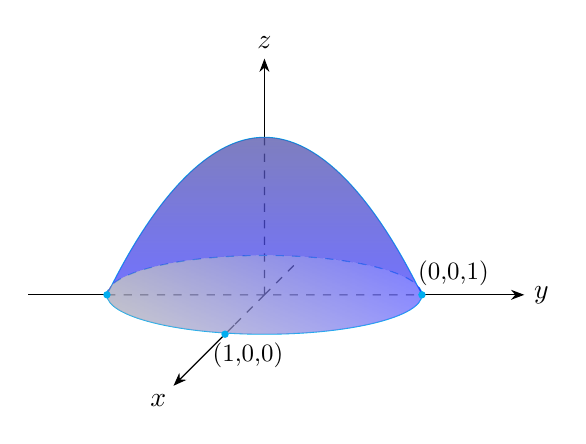
\begin{tikzpicture}[=>stealth]
\draw[dashed](-2,0,0)--(2,0,0)
(0,0,0)--(0,2,0)
(0,0,0)--(0,0,1)
(0,0,0)--(0,0,-1);
\draw[-Stealth](0,2,0)--(0,3,0)node[above]{$z$};
\draw[-Stealth](2,0,0)--(3.3,0,0)node[right]{$y$};
\draw[-Stealth](0,0,1)--(0,0,3);
\draw(-3,0,0)--(-2,0,0);
\draw[cyan](0,2)parabola(2,0)
(0,2)parabola(-2,0);
\draw[cyan](-2,0)arc(180:360:2cm and 0.5cm);
\draw[dashed,cyan](2,0)arc(0:180:2cm and 0.5cm);
%\path[fill=cyan,opacity=0.5](0,0)circle(2cm and 0.5cm)--(2,0)parabola[bend at end](0,2)--(0,2)parabola(-2,0);
\shade[top color=blue, opacity=0.5](0,2)parabola(2,0)--(2,0)arc(360:-180:2cm and 0.5cm)--(-2,0)parabola[bend at end](0,2)--cycle;
\shade[bottom color=blue,opacity=0.5](0,2)parabola(2,0)--(2,0)arc(0:180:2cm and 0.5cm)--(-2,0)parabola[bend at end](0,2)--cycle;
\shade[right color=blue,opacity=0.4](0,0)circle(2cm and 0.5cm);
\draw(2.4,0,0)node[above,scale=0.9]{(0,0,1)}
(2,0,0)node[shape=circle,scale=0.01cm, fill=cyan]{}
(-2,0,0)node[shape=circle,scale=0.01cm,fill=cyan]{}
(0,0,1.3)node[shape=circle,scale=0.01cm,fill=cyan]{}
(0,0,3.5)node[]{$x$}
(0,0,2)node[right,scale=0.9]{(1,0,0)};
\end{tikzpicture}
\end{figure}

{\color[wave]{485}\subsection{Level Curves}}

A second way to picture a function of two variables, often more useful than its
graph, is a contour map: the curves in the $xy$-plane on which $f$ is constant.

\begin{defn}
\label{defn:level}
The \emph{level curve} of $f$ at height $k$ is the set
\[\{(x,y)\in D : f(x,y) = k\},\]
for each $k$ in the range of $f$. For a function of three variables the same
definition gives a \emph{level surface} $f(x,y,z) = k$.
\end{defn}

As a point moves along a level curve the value of $f$ does not change. Drawing
the level curves for equally spaced values of $k$ and imagining each lifted to
height $k$ recovers the surface, exactly as contour lines on a map describe a
landscape; where the curves crowd together the surface is steep, and where they
spread out it is nearly flat.

For the hemisphere $z = \sqrt{1 - x^2 - y^2}$, setting $z = k$ gives
\[k = \sqrt{1 - x^2 - y^2} \iff x^2 + y^2 = 1 - k^2 ,\qquad 0\leq k\leq 1 .\]
So the level curves are circles centred at the origin: the unit circle at
height $k = 0$, shrinking to the single point $(0,0)$ at height $k = 1$. A value
such as $k = 2$ gives $x^2 + y^2 = -3$, which has no solutions, as it must:
$2$ is not in the range of $f$.

\begin{figure}[H]
\centering
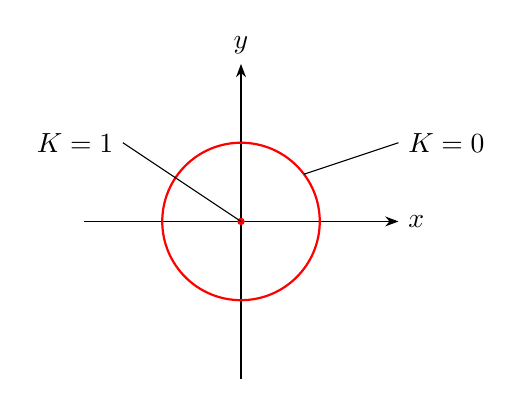
\begin{tikzpicture}[=>stealth]
\draw[-Stealth](-2,0)--(2,0)node[right]{$x$};
\draw[-Stealth](0,-2)--(0,2)node[above]{$y$};
\draw(0,0)node[shape=circle,fill=red,scale=0.01cm]{};
\draw[thick,red](0,0)circle [radius=1cm];
\draw(0,0)--(-1.5,1)node[left]{$K=1$};
\draw(0.8,0.6)--(2,1)node[right]{$K=0$};
\end{tikzpicture}
\end{figure}

\begin{exa}
\label{ex:levelg}
Let $g(x,y) = \sqrt{9 - x^2 - 2y^2}$.
\begin{enumerate}
\item Find the domain and range of $g$.

\item Sketch the level curves of $g$.
\end{enumerate}
\end{exa}

\begin{solution}
\begin{enumerate}
\item The square root requires $9 - x^2 - 2y^2\geq 0$, so
\[D = \{(x,y) \mid x^2 + 2y^2 \leq 9\},\]
the region inside and on the ellipse with semi-axes $3$ along the $x$-axis and
$\frac{3}{\sqrt2}$ along the $y$-axis. On $D$ the quantity $9 - x^2 - 2y^2$ takes
every value from $0$ (on the ellipse) to $9$ (at the origin), so the range is
$[0,3]$.

\item Setting $g = k$ gives
\[x^2 + 2y^2 = 9 - k^2 ,\qquad 0\leq k\leq 3,\]
a family of ellipses with the same shape: $k = 0$ gives the boundary
$x^2 + 2y^2 = 9$, $k = 1$ gives $x^2 + 2y^2 = 8$, $k = 2$ gives
$x^2 + 2y^2 = 5$, and $k = 3$ gives the single point $(0,0)$.

\begin{figure}[H]
\centering
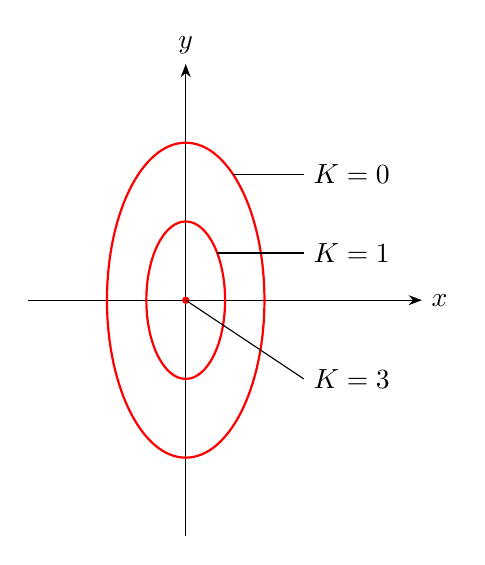
\begin{tikzpicture}[=>stealth]
\draw[-Stealth](0,-3)--(0,3)node[above]{$y$};
\draw[-Stealth](-2,0)--(3,0)node[right]{$x$};
\draw(0,0)node[shape=circle,fill=red,scale=0.01cm]{};
\draw[thick,red](0,0)ellipse[x radius=0.5cm, y radius=1cm];
\draw[thick,red](0,0)ellipse[x radius =1cm,y radius=2cm];
\draw(0,0)--(1.5,-1)node[right]{$K=3$};
\draw(0.6,1.6)--(1.5,1.6)node[right]{$K=0$};
\draw(0.4,0.6)--(1.5,0.6)node[right]{$K=1$};
\end{tikzpicture}
\end{figure}
\end{enumerate}
\end{solution}

\begin{exa}
\label{ex:domainln}
Find the domain and range of $f(x,y,z) = \ln (z-y) + xy\sin z$.
\end{exa}

\begin{solution}
The logarithm requires $z - y > 0$, and the second term is defined everywhere,
so
\[D = \{(x,y,z) \mid z > y\},\]
the open half-space lying above the plane $z = y$; $x$ is unrestricted. The
range is all of $\mathbb{R}$: already on the line $x = 0$, $y = 0$, $z>0$ the
function is $\ln z$, which takes every real value.

\begin{figure}[H]
\centering
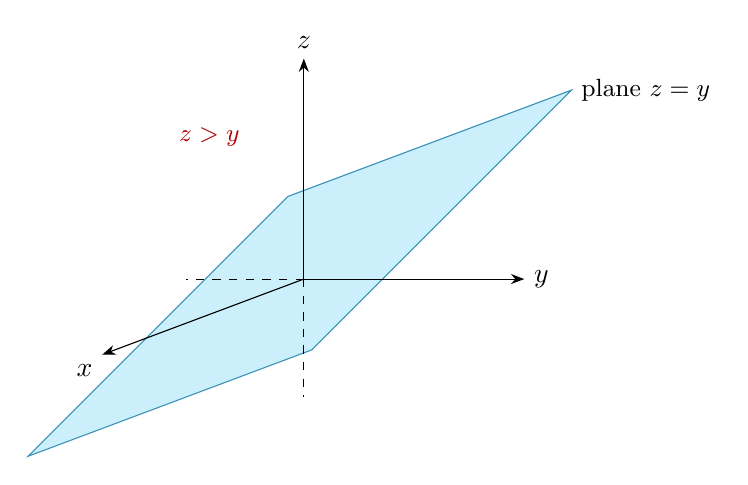
\begin{tikzpicture}[=>stealth,x={(-0.8cm,-0.3cm)},y={(1cm,0cm)},z={(0cm,1cm)}]
\fill[cyan!20] (-2,-1.5,-1.5)--(2.5,-1.5,-1.5)--(2.5,1.8,1.8)--(-2,1.8,1.8)--cycle;
\draw[cyan!70!black] (-2,-1.5,-1.5)--(2.5,-1.5,-1.5)--(2.5,1.8,1.8)--(-2,1.8,1.8)--cycle;
\draw[dashed](0,0,0)--(0,-1.5,0) (0,0,0)--(0,0,-1.5);
\draw[-Stealth](0,0,0)--(3.2,0,0)node[below left]{$x$};
\draw[-Stealth](0,0,0)--(0,2.8,0)node[right]{$y$};
\draw[-Stealth](0,0,0)--(0,0,2.8)node[above]{$z$};
\draw(-2,1.8,1.8)node[right,font=\small]{plane $z = y$};
\draw[red!70!black](0,-1.2,1.8)node[font=\small]{$z>y$};
\end{tikzpicture}
\end{figure}
\end{solution}


{\color[wave]{485}\subsection{Limits and Continuity}}

\begin{defn}
\label{defn:limit}
Let $f$ be defined on a set $D$ containing points arbitrarily close to
$(x_0,y_0)$. Then
\[\lim_{(x,y) \to (x_0,y_0)}f(x,y) = L\]
means: for every $\varepsilon>0$ there is a $\delta>0$ such that
\[|f(x,y) - L| < \varepsilon\quad\text{whenever}\quad (x,y)\in D\ \text{and}\
0 < \sqrt{(x-x_0)^2 + (y-y_0)^2} <\delta .\]
\end{defn}

In words, $f(x,y)$ can be made as close to $L$ as we please by taking $(x,y)$
inside a small enough disc about $(x_0,y_0)$, the centre itself excluded. The
condition says nothing about \emph{how} $(x,y)$ approaches $(x_0,y_0)$: every
point of the disc counts. That is what makes limits in the plane more delicate
than on the line.

\begin{defn}
\label{defn:continuous}
The function $f$ is \emph{continuous} at the point $P_0(x_0,y_0)$ if all three
of the following hold.
\begin{enumerate}
\item $f$ is defined at $P_0$; that is, $f(x_0,y_0)$ exists.

\item The limit
$\lim_{(x,y)\to (x_0,y_0)} f(x,y)$ exists.

\item The two agree:
$\lim_{(x,y)\to (x_0,y_0)} f(x,y) = f(x_0,y_0)$.
\end{enumerate}
The function $f$ is continuous on a set $S$ if it is continuous at every point
of $S$.
\end{defn}

The three conditions are independent, and a single example fails each of them in
turn: $f(x,y) = \frac{xy}{x^2+y^2}$ is undefined at the origin and so fails the
first; assigning it any value there still fails the second, since the limit does
not exist; and a function whose limit at $P_0$ exists but differs from its value
there fails only the third. This is the same three-part test as for one
variable. What is not the same is condition 2, and the difference is the whole
difficulty: on the line a point can be approached from two sides, in the plane
from infinitely many directions, and along curves as well as straight lines.

\begin{exa}
\label{ex:removable}
Let
\[f(x,y) =
\begin{cases}
3xy, & (x,y) \neq (1,2),\\
0, & (x,y) = (1,2).
\end{cases}\]
Then $f$ is defined at $(1,2)$, and since $3xy$ is a polynomial,
$\lim_{(x,y)\to (1,2)}f(x,y) = 3\cdot 1\cdot 2 = 6$. But $f(1,2) = 0\neq 6$, so
condition 3 fails and $f$ is not continuous at $(1,2)$.

Redefining the value there as $f(1,2) = 6$ makes the limit and the value agree,
and the new function, which is just $3xy$ everywhere, is continuous. A
discontinuity that can be removed in this way, by changing a single value, is
called \emph{removable}.
\end{exa}

\begin{exa}
\label{ex:nolimit}
Let $f(x,y) = \frac{xy}{x^2 + y^2}$ for $(x,y) \neq (0,0)$. Does $f$ have a limit
as $(x,y) \to (0,0)$?
\end{exa}

\begin{solution}
Approach the origin along the line $y = mx$. For $x\neq 0$,
\[f(x,mx) = \frac{x(mx)}{x^2 + (mx)^2} = \frac{m x^2}{x^2(1 +m^2)} =
\frac{m}{1 + m^2},\]
so on each line through the origin $f$ is constant, and the constant depends on
the line. Along $y = x$ it is $\frac{1}{2}$; along $y = 2x$ it is $\frac{2}{5}$.
If the limit existed and equalled $L$, every path would have to give $L$. Two
paths give different values, so the limit does not exist.
\end{solution}

The argument is worth isolating, since it is the standard tool for showing that
a limit does not exist.

\begin{prop}[Two-path test]
\label{prop:twopath}
If $f(x,y)\to L_1$ as $(x,y)\to(x_0,y_0)$ along one curve and $f(x,y)\to L_2$
along another, with $L_1\neq L_2$, then
$\lim_{(x,y)\to(x_0,y_0)} f(x,y)$ does not exist.
\end{prop}

\begin{proof}
If the limit existed and equalled $L$, then for any $\varepsilon>0$ all points of
$D$ in some punctured disc about $(x_0,y_0)$ would give values within
$\varepsilon$ of $L$, including the points of both curves. Hence both $L_1$ and
$L_2$ would equal $L$.
\end{proof}

The test can only ever prove that a limit fails to exist. To prove that a limit
\emph{does} exist, a bound valid for all points near $(x_0,y_0)$ is needed, and
the usual device is to compare with the distance
$r = \sqrt{(x-x_0)^2 + (y-y_0)^2}$, as in the next example.

\begin{exa}
\label{ex:continuityorigin}
Investigate the continuity at the origin of
\begin{enumerate}
\item $z = \frac{\sin (x+y)}{x + y}$, using $\lim_{t\to 0} \frac{\sin t}{t}=1$;

\item $z = \frac{xy}{x^2 + y^2}$.
\end{enumerate}
\end{exa}

\begin{solution}
\begin{enumerate}
\item The function is undefined wherever $x + y = 0$, which includes the origin,
so it is not continuous there as it stands. Its limit does exist: with
$t = x + y$, which tends to $0$ as $(x,y)\to (0,0)$,
\[\lim_{(x,y)\to(0,0)}\frac{\sin(x+y)}{x+y} = \lim_{t\to 0}\frac{\sin t}{t} = 1 .\]
So the discontinuity is removable: defining $z = 1$ on the line $x + y = 0$ gives
a function continuous everywhere.

\item By Example~\ref{ex:nolimit} the limit at the origin does not exist, so no
choice of value at the origin can make this function continuous there.
\end{enumerate}
\end{solution}

\subhead{Extension to Three or More Variables}

For a function of three variables,
$\lim_{(x,y,z)\to (a,b,c)}f(x,y,z) =L$ means that $|f(x,y,z) - L|<\varepsilon$
whenever $0 < \sqrt{(x-a)^2 + (y-b)^2 + (z-c)^2} < \delta$: the disc is replaced by
a ball. Continuity is defined by the same three conditions, and the same rules
hold. Sums, products and quotients of continuous functions are continuous where
the denominator is non-zero, and so are compositions of continuous functions. In
particular every polynomial is continuous everywhere, and every rational
function is continuous wherever its denominator is non-zero.

For example,
\[f(x,y,z) = \frac{1}{x^2 + y^2 + z^2 - 1}\]
is a rational function of three variables, continuous everywhere in
$\mathbb{R}^3$ except where $x^2 + y^2 + z^2 = 1$: it is discontinuous exactly on
the sphere with centre $(0,0,0)$ and radius $1$.

\begin{exa}
\label{ex:limitexists}
Show that $\lim_{(x,y)\to(0,0)}\frac{3x^2y}{x^2+y^2} = 0$.
\end{exa}

\begin{solution}
Every straight line through the origin gives $0$, but that proves nothing, so a
bound is needed. Since $x^2\leq x^2+y^2$,
\[\left|\frac{3x^2y}{x^2+y^2}\right| = 3|y|\,\frac{x^2}{x^2+y^2}\leq 3|y|\leq
3\sqrt{x^2+y^2} .\]
Given $\varepsilon>0$, take $\delta = \frac{\varepsilon}{3}$. Then
$0<\sqrt{x^2+y^2}<\delta$ gives $|f(x,y) - 0|<3\delta = \varepsilon$, so the limit
is $0$. Defining $f(0,0) = 0$ makes $f$ continuous at the origin.
\end{solution}

\begin{exa}
\label{ex:polar}
Decide whether $\lim_{(x,y)\to(0,0)}\frac{x^2-y^2}{\sqrt{x^2+y^2}}$ exists.
\end{exa}

\begin{solution}
Polar coordinates turn the question into one about a single variable. With
$x = r\cos\theta$ and $y = r\sin\theta$,
\[\frac{x^2-y^2}{\sqrt{x^2+y^2}} = \frac{r^2(\cos^2\theta - \sin^2\theta)}{r} =
r\cos 2\theta .\]
Since $|r\cos 2\theta|\leq r$ for every $\theta$, the expression tends to $0$ as
$r\to 0$, whatever the direction, curved or straight. The limit exists and
equals $0$. The method works because the bound $r$ does not depend on $\theta$;
had the result been $\cos 2\theta$ alone, with no factor $r$, the limit would
have failed to exist.
\end{solution}

\begin{exa}
\label{ex:parabolapath}
Show that $\lim_{(x,y)\to(0,0)}\frac{x^2y}{x^4+y^2}$ does not exist, even though
the function tends to $0$ along every straight line through the origin.
\end{exa}

\begin{solution}
Along the line $y = mx$ with $m\neq 0$,
\[\frac{x^2(mx)}{x^4 + m^2x^2} = \frac{mx}{x^2+m^2}\to 0 ,\]
and along both axes the function is identically $0$. Along the parabola
$y = x^2$, however,
\[\frac{x^2\cdot x^2}{x^4 + x^4} = \frac12\quad\text{for every } x\neq 0 .\]
By Proposition~\ref{prop:twopath} the limit does not exist. The parabola is the
natural path to try because it makes the two terms $x^4$ and $y^2$ of the
denominator the same size.
\end{solution}


{\color[wave]{485}\subsection{Directional Derivatives and Gradient Vector}}

The partial derivatives
\[f_x(x_0,y_0) = \lim_{h\to 0} \frac{f(x_0 + h, y_0) - f(x_0,y_0)}{h},\qquad
f_y(x_0,y_0) = \lim_{h\to 0} \frac{f(x_0, y_0 +h) - f(x_0,y_0)}{h}\]
are the rates of change of $f$ in the directions of the unit vectors $\mathbf i$
and $\mathbf j$. Two directions are not enough to describe a surface, and the
existence of both partial derivatives is a weak condition: the function
$\frac{xy}{x^2+y^2}$ of Example~\ref{ex:nolimit}, given the value $0$ at the
origin, has $f_x(0,0) = f_y(0,0) = 0$ (it vanishes on both axes) and yet is not
even continuous there. The condition that does the work is the following.

\begin{defn}
\label{defn:differentiable}
A function $f$ of two variables is \emph{differentiable} at $(x_0,y_0)$ if both
partial derivatives exist there and
\[f(x_0+h,y_0+k) = f(x_0,y_0) + f_x(x_0,y_0)\,h + f_y(x_0,y_0)\,k +
\varepsilon(h,k)\sqrt{h^2+k^2},\]
where $\varepsilon(h,k)\to 0$ as $(h,k)\to(0,0)$.
\end{defn}

In words, near $(x_0,y_0)$ the function is the linear function
$f(x_0,y_0) + f_x h + f_y k$ plus an error that is small compared with the
distance moved. The graph of that linear function is the \emph{tangent plane}
\[z = f(x_0,y_0) + f_x(x_0,y_0)(x-x_0) + f_y(x_0,y_0)(y-y_0).\]
Two facts make the definition easy to use. A differentiable function is
continuous, since the right-hand side tends to $f(x_0,y_0)$ as
$(h,k)\to(0,0)$. And if $f_x$ and $f_y$ exist near $(x_0,y_0)$ and are
continuous at that point, then $f$ is differentiable there; the proof applies the
one-variable mean value theorem once in each variable. So every function built
from polynomials, exponentials, logarithms and trigonometric functions is
differentiable wherever its partial derivatives are continuous.

\begin{defn}
\label{defn:directional}
The \emph{directional derivative} of $f$ at $(x_0,y_0)$ in the direction of the
unit vector $\mathbf u = \langle a, b\rangle = a\,\mathbf i + b\,\mathbf j$ is
\[D_{\mathbf u} f(x_0,y_0) = \lim_{h\to 0} \frac{f(x_0 + ha, y_0+hb) -
f(x_0,y_0)}{h},\]
when the limit exists.
\end{defn}

It is the rate of change of $f$ per unit distance as $(x,y)$ moves from
$(x_0,y_0)$ in the direction $\mathbf u$. Taking $\mathbf u = \mathbf i$ gives
$f_x$, and $\mathbf u = \mathbf j$ gives $f_y$. The vector must be a unit
vector, or the rate would be measured per some other unit of length.

\begin{thm}
\label{thm:directional}
If $f$ is differentiable at $(x,y)$, then $f$ has a directional derivative there
in the direction of every unit vector $\mathbf u = \langle a, b \rangle$, and
\[D_{\mathbf u}f(x,y) = f_x(x,y)\, a + f_y(x,y)\, b .\]
\end{thm}

\begin{proof}
Apply Definition~\ref{defn:differentiable} with $h$ replaced by $ta$ and $k$ by
$tb$. Since $a^2+b^2 = 1$, the distance moved is
$\sqrt{t^2a^2+t^2b^2} = |t|$, so
\[f(x+ta,y+tb) - f(x,y) = t\,(f_x a + f_y b) + \varepsilon(ta,tb)\,|t| .\]
Dividing by $t$,
\[\frac{f(x+ta,y+tb) - f(x,y)}{t} = f_x a + f_y b \pm \varepsilon(ta,tb),\]
and the last term tends to $0$ as $t\to 0$.
\end{proof}

\begin{exa}
\label{ex:dirangle}
Let $f(x,y) = x^3 -3xy + 4y^2$. Find the directional derivative of $f$ at $(1,2)$
in the direction of the unit vector $\mathbf u$ making the angle
$\theta = \frac{\pi}{6}$ with the positive $x$-axis.
\end{exa}

\begin{solution}
The partial derivatives are
\[f_x = 3x^2 -3y ,\qquad f_y = -3x + 8y ,\]
and the unit vector at angle $\theta$ is
$\mathbf u = \langle\cos\theta,\sin\theta\rangle$, so here
$a = \cos \frac{\pi}{6} = \frac{\sqrt 3}{2}$ and $b = \sin \frac{\pi}{6} = \frac12$.

\begin{figure}[H]
\centering
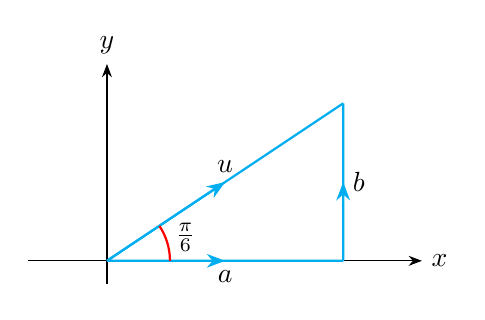
\begin{tikzpicture}[=>stealth]
\draw[-Stealth](-1,0)--(4,0)node[right]{$x$};
\draw[-Stealth](0,-0.3)--(0,2.5)node[above]{$y$};
\draw[thick,cyan,-Stealth](0,0)--(1.5,1);
\draw[thick,cyan,-Stealth](3,0)--(3,1);
\draw[thick,cyan,-Stealth](0,0)--(1.5,0);
\draw[thick,cyan](0,0)--(3,0)
(3,0)--(3,2)
(0,0)--(3,2);
\draw(1.5,0)node[below]{$a$}
(3,1)node[right]{$b$}
(1.5,1)node[above]{$u$};
\coordinate (a) at (0.5,0);
\coordinate (b) at (0,0);
\coordinate (c) at (0.5,0.33);
\draw
pic[thick,draw=red,-,angle radius=0.8cm,"$\frac{\pi}{6}$",angle eccentricity = 1.3]{angle=a--b--c};
\end{tikzpicture}
\end{figure}

By Theorem~\ref{thm:directional},
\begin{align*}
D_{\mathbf u} f(x,y) & = (3x^2 - 3y) \frac{\sqrt3}{2} + (-3x + 8y) \frac{1}{2},\\
D_{\mathbf u} f(1,2) & = (3 - 6)\frac{\sqrt3}{2} + (-3 + 16)\frac12 =
\frac{13 - 3\sqrt{3}}{2}\approx 3.90 .
\end{align*}
\end{solution}

\subhead{Gradient Vector}

The formula of Theorem~\ref{thm:directional} is a dot product, and naming the
vector that appears in it is the most useful single step in this section.

\begin{defn}
\label{defn:gradient}
If $f$ is a function of two variables $x$ and $y$, the \emph{gradient} of $f$ is
the vector
\[\nabla f = \frac{\partial f}{\partial x}\,\mathbf i +\frac{\partial f}{\partial
y}\,\mathbf j = \langle f_x , f_y\rangle .\]
For a function of three variables,
$\nabla f = \langle f_x, f_y, f_z\rangle$.
\end{defn}

With it, Theorem~\ref{thm:directional} reads
\[D_{\mathbf u}f = f_x\, a + f_y\, b = \langle f_x , f_y\rangle \cdot \langle
a,b\rangle = \nabla f\cdot\mathbf u ,\]
and the same proof gives $D_{\mathbf u}f = \nabla f\cdot\mathbf u$ in three
variables, where the directional derivative at $(x_0,y_0,z_0)$ in the direction
of the unit vector $\mathbf u = \langle a,b,c\rangle$ is
\[D_{\mathbf u}f(x_0,y_0,z_0) = \lim_{h\to 0}\frac{f(x_0 + ha, y_0 + hb, z_0 +
hc) - f(x_0,y_0,z_0)}{h} .\]

\begin{exa}
\label{ex:gradsin}
If $f(x,y) = \sin x + e^{xy}$, find $\nabla f$, and its value at $(0,1)$.
\end{exa}

\begin{solution}
\[\nabla f = \langle f_x, f_y\rangle = \langle \cos x + ye^{xy},\ xe^{xy}\rangle,
\qquad \nabla f (0,1) = \langle 1 + 1,\ 0\rangle = \langle 2,0\rangle .\]
\end{solution}

\begin{exa}
\label{ex:dirvector}
Find the directional derivative of $f(x,y) = x^2y^3 -4y$ at the point $(2,-1)$
in the direction of the vector $\mathbf v = 2\,\mathbf i + 5\,\mathbf j$.
\end{exa}

\begin{solution}
\[\nabla f (x,y) = \langle 2xy^3,\ 3x^2y^2 -4\rangle ,\qquad \nabla f (2,-1) =
\langle -4,\ 8\rangle .\]
The given vector is not a unit vector, so it is normalised first:
\[\mathbf u = \frac{\mathbf v}{|\mathbf v|} = \frac{1}{\sqrt{29}}\langle 2,
5\rangle .\]
Then
\[D_{\mathbf u}f(2,-1) = \nabla f (2,-1)\cdot\mathbf u = \frac{-8 + 40}{\sqrt{29}}
= \frac{32}{\sqrt{29}} = \frac{32\sqrt{29}}{29}\approx 5.94 .\]
\end{solution}

\begin{exa}
\label{ex:dir3}
Let $f(x,y,z) = x\sin yz$.
\begin{enumerate}
\item Find the gradient of $f$.

\item Find the directional derivative of $f$ at $(1,3,0)$ in the direction of
$\mathbf v = \mathbf i + 2\,\mathbf j -\mathbf k$.
\end{enumerate}
\end{exa}

\begin{solution}
\begin{enumerate}
\item
\[\nabla f = \langle \sin yz,\ xz\cos yz,\ xy\cos yz\rangle .\]

\item At $(1,3,0)$, $\sin yz = 0$ and $\cos yz = 1$, so
$\nabla f(1,3,0) = \langle 0, 0, 3\rangle$. The unit vector is
$\mathbf u = \frac{1}{\sqrt{6}}\langle 1, 2, -1\rangle$, so
\[D_{\mathbf u} f(1,3,0) = \langle 0,0,3\rangle\cdot\frac{1}{\sqrt6}\langle
1,2,-1\rangle = -\frac{3}{\sqrt6} = -\sqrt{\frac{3}{2}}\approx -1.22 .\]
\end{enumerate}
\end{solution}

\begin{exa}
\label{ex:tangentplane}
Find the tangent plane to $z = x^2 + xy - y^2$ at $(1,2)$, and use it to estimate
$f(1.1, 1.95)$.
\end{exa}

\begin{solution}
Here $f(1,2) = 1 + 2 - 4 = -1$, $f_x = 2x + y = 4$ and $f_y = x - 2y = -3$ at
$(1,2)$. The tangent plane is
\[z = -1 + 4(x-1) - 3(y-2).\]
At $(1.1,1.95)$ it gives $-1 + 4(0.1) - 3(-0.05) = -0.45$. The exact value is
$1.21 + 2.145 - 3.8025 = -0.4475$, so the linear approximation is in error by
$0.0025$, which is of the order of the square of the step, as
Definition~\ref{defn:differentiable} predicts.
\end{solution}

\begin{exa}
\label{ex:notdifferentiable}
Let $f(x,y) = \frac{xy}{x^2+y^2}$ for $(x,y)\neq(0,0)$ and $f(0,0) = 0$. Show
that $f_x(0,0)$ and $f_y(0,0)$ exist but that $f$ has no directional derivative
at the origin in the direction $\mathbf u = \frac{1}{\sqrt2}\langle 1,1\rangle$.
\end{exa}

\begin{solution}
On the $x$-axis $f(h,0) = 0$, so $f_x(0,0) = \lim_{h\to 0}\frac{0-0}{h} = 0$, and
likewise $f_y(0,0) = 0$. In the diagonal direction,
\[\frac{f\left(\frac{h}{\sqrt2},\frac{h}{\sqrt2}\right) - f(0,0)}{h} =
\frac{1}{h}\cdot\frac{h^2/2}{h^2} = \frac{1}{2h},\]
which has no limit as $h\to 0$. If $f$ were differentiable at the origin,
Theorem~\ref{thm:directional} would give the directional derivative
$0\cdot\frac{1}{\sqrt2} + 0\cdot\frac{1}{\sqrt2} = 0$, so $f$ is not
differentiable there. Partial derivatives alone do not make a function
differentiable.
\end{solution}

{\color[wave]{485}\subsection{Maximising the Directional Derivative}}

Of all the directions in which one can move from a point, in which does $f$
increase fastest, and how fast? The gradient answers both questions.

\begin{thm}[Maximising the directional derivative]
\label{thm:maxdir}
Let $f$ be a differentiable function of two or three variables. At any point
$\mathbf x$ the largest value taken by the directional derivative
$D_{\mathbf u}f(\mathbf x)$, as the unit vector $\mathbf u$ ranges over all
directions, is $|\nabla f(\mathbf x)|$, and if $\nabla f(\mathbf x)\neq\mathbf
0$ it is attained exactly when $\mathbf u$ points in the direction of
$\nabla f(\mathbf x)$.
\end{thm}

\begin{proof}
Write $\theta$ for the angle between $\nabla f$ and $\mathbf u$. Since
$\mathbf u$ is a unit vector,
\[D_{\mathbf u} f = \nabla f\cdot\mathbf u = |\nabla f|\,|\mathbf u|\, \cos
\theta = |\nabla f|\cos \theta .\]
Only $\cos\theta$ depends on the direction chosen, and $\cos\theta$ is largest,
equal to $1$, exactly when $\theta = 0$. Hence the maximum value is $|\nabla f|$,
attained when $\mathbf u$ is parallel to $\nabla f$.
\end{proof}

The same one-line calculation settles the other two directions at once, and it
is worth reading off all three together:
\begin{enumerate}
\item[$-$] $\theta = 0$: the derivative is $+|\nabla f|$. The gradient
points in the direction of \emph{steepest ascent}.

\item[$-$] $\theta = \frac{\pi}{2}$: the derivative is $0$. Perpendicular to
the gradient the function does not change to first order --- which is exactly
why the level curves of $f$ cross the gradient at right angles.

\item[$-$] $\theta = \pi$: the derivative is $-|\nabla f|$, the
direction of \emph{steepest descent}.
\end{enumerate}
So a single vector, $\nabla f$, answers three questions: which way is uphill,
which way is flat, and how steep the hill is.

\begin{figure}[H]
\centering
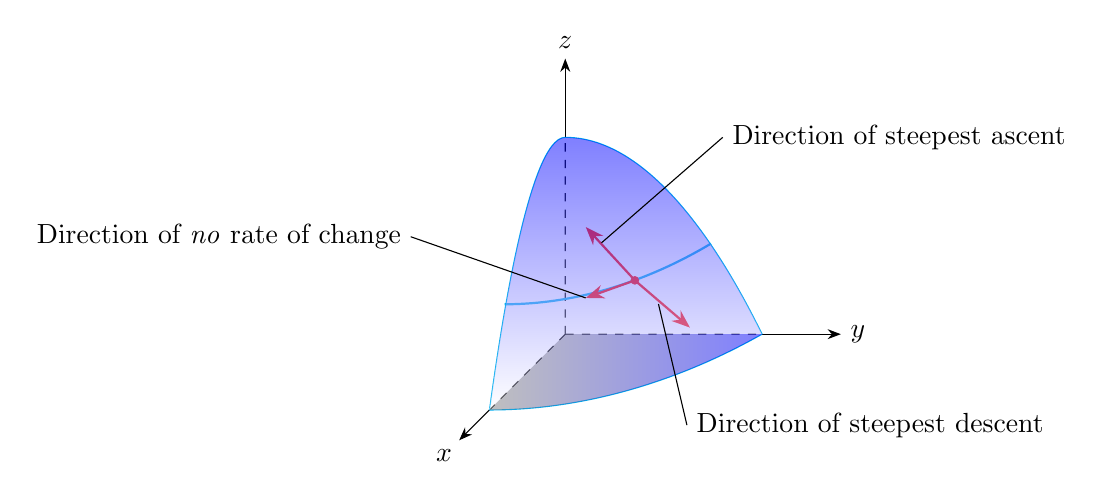
\begin{tikzpicture}[=>stealth]
\draw[-Stealth](2.5,0,0)--(3.5,0,0)node[right]{$y$};
\draw[-Stealth](0,2.5,0)--(0,3.5,0)node[above]{$z$};
\draw[-Stealth](0,0,2.5)--(0,0,3.5);
\draw(0,0,4)node[]{$x$};
\draw[dashed](0,0,0)--(2.5,0,0)
(0,0,0)--(0,2.5,0)
(0,0,0)--(0,0,2.5);
\draw[cyan](2.5,0,0)parabola[bend at end](0,0,2.5)
(0,0,2.5)parabola[bend at  end](0,2.5,0)
(2.5,0,0)parabola[bend at end](0,2.5,0);
\draw[thick,cyan](0,1.15,2)parabola(1.85,1.15,0);
\draw(2,1.8,2.9)node[shape=circle,fill=red,draw=red,scale=0.01cm]{};
\draw[-Stealth,thick,red](2,1.8,2.9)--(1.3,2.4,2.7);
\draw[-Stealth,thick,red](2,1.8,2.9)--(2.7,1.2,2.9);
\draw[-Stealth,thick,red](2,1.8,2.9)--(1.8,2,4);
\shade[top color=blue,opacity=0.5](0,2.5,0)parabola(2.5,0,0)--(2.5,0,0)--(0,0,0)--(0,2.5,0)--cycle
(0,2.5,0)parabola(0,0,2.5)--(0,0,2.5)--(0,0,0)--(0,2.5,0)--cycle;
\shade[right color=blue,opacity=0.5](2.5,0,0)parabola[bend at end](0,0,2.5)--(0,0,2.5)--(0,0,0)--(2.5,0,0)--cycle;
\draw(1.5,2.2,2.7)--(2,2.5,0)node[right]{Direction of steepest ascent};
\draw(1.8,2,4)--(-1,2.2,2.5)node[left]{Direction of \textit{no} rate of change};
\draw(2.3,1.5,2.9)--(2.7,0,3)node[right]{Direction of steepest descent};
%\shade[top color=blue,opacity=0.4](0,2.5,0)parabola(2.5,0,0)--(2.5,0,0)parabola[bend at end](0,0,2.5)--(0,0,2.5)parabola[bend at end](0,2.5,0)--cycle;
\end{tikzpicture}
\end{figure}

\begin{exa}
\label{ex:xey}
Let $f(x,y) = xe^y$.
\begin{enumerate}
\item Find the rate of change of $f$ at the point $P(2,0)$ in the direction from
$P$ to $Q\left(\frac12,2\right)$.

\item In what direction does $f$ have the maximum rate of change at $P$? What is
that maximum?
\end{enumerate}
\end{exa}

\begin{solution}
\begin{enumerate}
\item $\nabla f = \langle e^y,\ xe^y\rangle$, so $\nabla f(2,0) = \langle 1,
2\rangle$. The vector from $P$ to $Q$ is $\overrightarrow{PQ} =
\left\langle -\frac32, 2\right\rangle$, of length $\frac52$, so the unit vector is
$\mathbf u = \left\langle -\frac{3}{5},\frac{4}{5}\right\rangle$ and
\[D_{\mathbf u} f(2,0) = \langle 1,2\rangle\cdot \left\langle
-\frac{3}{5},\frac{4}{5}\right\rangle = -\frac35 + \frac85 = 1 .\]

\item By Theorem~\ref{thm:maxdir}, $f$ increases fastest in the direction of
$\nabla f(2,0) = \langle 1,2\rangle$, and the maximum rate is
$|\langle 1,2\rangle| = \sqrt{5}\approx 2.24$.
\end{enumerate}
\end{solution}

\begin{exa}
\label{ex:temperature}
Suppose that the temperature at a point $(x,y,z)$ in space is
\[T(x,y,z) = \frac{80}{1 + x^2 + 2y^2 + 3z^2},\]
where $T$ is measured in degrees Celsius and $x,y,z$ in metres. In which
direction does the temperature increase fastest at the point $(1,1,-2)$? What is
the maximum rate of increase?
\end{exa}

\begin{solution}
Writing $s = 1 + x^2 + 2y^2 + 3z^2$, so that $T = 80s^{-1}$,
\[\nabla T = -\frac{80}{s^2}\nabla s = -\frac{80}{s^2}\langle 2x, 4y,
6z\rangle = \frac{160}{s^2}\langle -x, -2y, -3z\rangle .\]
At $(1,1,-2)$, $s = 1 + 1 + 2 + 12 = 16$, so
\[\nabla T (1,1,-2) = \frac{160}{256}\langle -1, -2, 6\rangle = \frac{5}{8}\langle
-1,-2,6\rangle .\]
The temperature increases fastest in the direction of $\langle -1,-2,6\rangle$,
that is, of the unit vector $\frac{1}{\sqrt{41}}\langle -1,-2,6\rangle$. The
maximum rate of increase is
\[|\nabla T(1,1,-2)| = \frac{5}{8}\sqrt{1 + 4 + 36} = \frac{5\sqrt{41}}{8}
\approx 4.0\ ^{\circ}\text{C per metre}.\]
\end{solution}

\begin{exe}
\label{exe:ln}
Find the directional derivative of $f(x,y,z) = \ln(1 + x^2 + y^2 + z^2)$ at the
point $P(1,-1,1)$ in the direction of the vector $\mathbf v = \langle 2,-2,
-3\rangle$.

\textbf{Answer:} $\nabla f = \frac{2}{1 + x^2+y^2+z^2}\langle x,y,z\rangle$, so
$\nabla f(1,-1,1) = \frac12\langle 1,-1,1\rangle$, and with
$\mathbf u = \frac{1}{\sqrt{17}}\langle 2,-2,-3\rangle$,
$D_{\mathbf u}f(P) = \frac{2 + 2 - 3}{2\sqrt{17}} = \frac{1}{2\sqrt{17}}\approx
0.121$.
\end{exe}

\begin{exa}
\label{ex:normal}
Show that the gradient is perpendicular to the level curves, and use this to find
a normal vector and the tangent line to the ellipse $x^2 + 4y^2 = 8$ at $(2,1)$.
\end{exa}

\begin{solution}
Let $\mathbf r(t) = \langle x(t),y(t)\rangle$ be a curve lying in the level curve
$f(x,y) = k$, so that $f(x(t),y(t)) = k$ for all $t$. Differentiating with the
chain rule of the subsection on composite functions,
\[f_x\,x'(t) + f_y\,y'(t) = 0,\qquad\text{that is}\qquad \nabla f\cdot\mathbf
r'(t) = 0 ,\]
so $\nabla f$ is perpendicular to the tangent vector of the level curve.

For $f(x,y) = x^2 + 4y^2$, $\nabla f = \langle 2x, 8y\rangle$, which is
$\langle 4,8\rangle$ at $(2,1)$. So $\langle 1,2\rangle$ is normal to the ellipse
there, and the tangent line is
\[1\,(x-2) + 2\,(y-1) = 0,\qquad\text{or}\qquad x + 2y = 4 .\]
\end{solution}

\begin{exa}
\label{ex:heatseeking}
A heat-seeking particle moves on a metal plate whose temperature is
$T(x,y) = 100 - x^2 - 2y^2$, always in the direction of the gradient. Find its
path if it starts at $(2,1)$.
\end{exa}

\begin{solution}
The velocity is parallel to $\nabla T = \langle -2x, -4y\rangle$, so along the
path $\frac{dy}{dx} = \frac{-4y}{-2x} = \frac{2y}{x}$. Separating the variables,
$\frac{dy}{y} = \frac{2\,dx}{x}$, so $\ln|y| = 2\ln|x| + C$ and $y = cx^2$. The
start $(2,1)$ gives $c = \frac14$. The particle follows the parabola
$y = \frac{x^2}{4}$ towards the hottest point, the origin, crossing every
isotherm $x^2 + 2y^2 = \text{constant}$ at right angles.
\end{solution}


{\color[wave]{485}\subsection{Maximum and Minimum Values}}

\begin{defn}
\label{defn:localext}
A function $f$ of two variables has a \emph{local maximum} at $(a,b)$ if
$f(x,y)\leq f(a,b)$ for all $(x,y)$ in some disc centred at $(a,b)$; the number
$f(a,b)$ is a \emph{local maximum value}. If instead $f(x,y)\geq f(a,b)$ on such
a disc, $f$ has a \emph{local minimum} at $(a,b)$. If the inequality holds for
all $(x,y)$ in the domain, the maximum or minimum is \emph{absolute}.
\end{defn}

\begin{thm}
\label{thm:fermat}
If $f$ has a local maximum or minimum at $(a,b)$ and the first partial
derivatives of $f$ exist there, then
\[f_x(a,b) = 0 ,\qquad f_y(a,b) = 0 .\]
\end{thm}

\begin{proof}
The function of one variable $g(x) = f(x,b)$ has a local maximum or minimum at
$x = a$, so $g'(a) = 0$ by the one-variable result; but $g'(a) = f_x(a,b)$. The
same argument with $h(y) = f(a,y)$ gives $f_y(a,b) = 0$.
\end{proof}

A point $(a,b)$ at which $f_x(a,b)=0$ and $f_y(a,b) =0$, or at which one of the
partial derivatives does not exist, is a \emph{critical point} (or
\emph{stationary point} when both derivatives vanish). Theorem~\ref{thm:fermat}
says that local extrema occur only at critical points. The converse is false: at
a critical point a function may have a maximum, a minimum, or neither, as the
next two examples show.

\begin{exa}
\label{ex:completesquare}
Let $f(x,y) = x^2 + y^2 - 2x -6y + 14$. Find and classify the critical points.
\end{exa}

\begin{solution}
\[f_x = 2x -2 = 0 ,\qquad f_y = 2y - 6 =0 ,\]
so $(1,3)$ is the only critical point. Completing the squares,
\[f(x,y) = (x-1)^2 + (y-3)^2 + 4 .\]
Both squares are non-negative, so $f(x,y)\geq 4 = f(1,3)$ for all $(x,y)$. The
point $(1,3)$ is a local minimum, and in fact an absolute minimum: the graph is a
paraboloid with vertex $(1,3,4)$.
\end{solution}

\begin{exa}
\label{ex:saddle}
Find the extreme values of $f(x,y) = y^2 - x^2$.
\end{exa}

\begin{solution}
$f_x = -2x$ and $f_y = 2y$ vanish only at $(0,0)$, where $f = 0$. On the
$x$-axis, $f(x,0) = -x^2 <0$ for $x\neq 0$; on the $y$-axis, $f(0,y) = y^2> 0$
for $y\neq 0$. So every disc about the origin contains points where $f$ is above
$0$ and points where it is below, and $f(0,0) = 0$ is neither a maximum nor a
minimum. The surface is a hyperbolic paraboloid, and the origin is a
\emph{saddle point}: a maximum along one axis and a minimum along the other.
\end{solution}

\subhead{Second Derivative Test}

\begin{thm}[Second derivative test]
\label{thm:secondderiv}
Suppose the second partial derivatives of $f$ are continuous on a disc centred at
$(a,b)$, and that $f_x(a,b)=0$ and $f_y(a,b) =0$. Let
\[D = D(a,b) = \begin{vmatrix} f_{xx} & f_{xy}\\ f_{xy} & f_{yy}\end{vmatrix} =
f_{xx}(a,b)f_{yy}(a,b) -f_{xy}(a,b)^2 .\]
\begin{enumerate}
\item If $D> 0$ and $f_{xx}(a,b)>0$, then $f(a,b)$ is a local minimum.

\item If $D>0$ and $f_{xx}(a,b)<0$, then $f(a,b)$ is a local maximum.

\item If $D<0$, then $(a,b)$ is a saddle point: $f(a,b)$ is neither a maximum
nor a minimum.
\end{enumerate}
If $D = 0$ the test gives no information.
\end{thm}

\begin{proof}
Fix a direction $(h,k)$ and put $g(t) = f(a+th,b+tk)$. By the chain rule (the
subsection on composite functions),
\[g'(t) = f_x h + f_y k,\qquad g''(t) = f_{xx}h^2 + 2f_{xy}hk + f_{yy}k^2 =
Q(h,k),\]
with the derivatives evaluated at $(a+th,b+tk)$. When $f_{xx}\neq 0$, completing
the square gives
\[f_{xx}\,Q(h,k) = (f_{xx}h + f_{xy}k)^2 + (f_{xx}f_{yy} - f_{xy}^2)\,k^2 .\]

Suppose $D>0$ and $f_{xx}(a,b)>0$. By continuity of the second derivatives,
$f_{xx}>0$ and $f_{xx}f_{yy} - f_{xy}^2>0$ on some smaller disc $B$ about
$(a,b)$. On $B$ both terms on the right are non-negative and they are not both
zero unless $h = k = 0$, so $Q(h,k)>0$. Now let $(a+h,b+k)$ be any other point of
$B$. Then $g'(0) = f_x(a,b)h + f_y(a,b)k = 0$ and $g''(t)>0$ for $0\leq t\leq 1$,
so $g'$ is increasing, $g'(t)>0$ for $0<t\leq 1$, and $g(1)>g(0)$; that is,
$f(a+h,b+k)>f(a,b)$. This proves part 1, and part 2 follows by applying it to
$-f$.

If $D<0$, then $Q(1,0) = f_{xx}(a,b)$ and $Q(-f_{xy},f_{xx}) =
f_{xx}D$ have opposite signs when $f_{xx}(a,b)\neq 0$ (and if $f_{xx}(a,b) =
0$, then $f_{xy}(a,b)\neq 0$ and $Q(1,s)$ takes both signs for suitable $s$).
So $g''(0)>0$ in one direction and $g''(0)<0$ in another: along the first line
$f$ has a strict local minimum at $(a,b)$, along the second a strict local
maximum, and $(a,b)$ is a saddle point.
\end{proof}

The quantity $Q(h,k)$ is the second-order term of the Taylor expansion of the
subsection on Taylor's formula, so the test says that near a critical point the
function looks like the quadratic $Q$: a bowl when $D>0$ and $f_{xx}>0$, an
inverted bowl when $D>0$ and $f_{xx}<0$, and a saddle when $D<0$.

\begin{exa}
\label{ex:quartic}
Find the local maximum and minimum values and saddle points of
\[f(x,y) = x^4 + y^4 - 4xy + 1 .\]
\end{exa}

\begin{solution}
\[f_x = 4x^3 - 4y =0,\qquad f_y = 4y^3 - 4x =0 ,\]
so $y =x^3$ and $x = y^3$. Substituting the first into the second,
\[0 = x^9 -x = x(x^8 -1) = x(x^4 + 1)(x^2 + 1)(x + 1)(x -1),\]
whose real roots are $x = 0, 1, -1$, with $y = x^3 = 0, 1, -1$. The critical
points are $(0,0)$, $(1,1)$ and $(-1,-1)$. The second derivatives are
\[f_{xx} = 12x^2,\qquad f_{xy} = -4,\qquad f_{yy} = 12y^2,\qquad
D = 144x^2y^2 - 16 .\]
\begin{enumerate}
\item[$-$] At $(0,0)$, $D = -16<0$: a saddle point, with $f(0,0) = 1$.
\item[$-$] At $(1,1)$, $D = 128>0$ and $f_{xx} = 12>0$: a local minimum, with
$f(1,1) = -1$.
\item[$-$] At $(-1,-1)$, $D = 128>0$ and $f_{xx} = 12>0$: a local minimum, with
$f(-1,-1) = -1$.
\end{enumerate}
\end{solution}

\begin{exa}
\label{ex:distanceplane}
Find the shortest distance from the point $(1,0,-2)$ to the plane
$x + 2y + z = 4$.
\end{exa}

\begin{solution}
A point of the plane has $z = 4 - x - 2y$, and its distance from $(1,0,-2)$ is
\[d = \sqrt{(x-1)^2 + y^2 + (6-x-2y)^2} .\]
It is simpler to minimise $f = d^2$, which has its minimum at the same point:
\[f(x,y) = (x-1)^2 + y^2 + (6-x-2y)^2 .\]
Then
\[f_x = 2(x -1) -2(6 - x -2y) = 4x + 4y - 14,\qquad f_y = 2y - 4(6 - x - 2y) =
4x + 10y - 24 .\]
Setting both to zero and subtracting gives $6y = 10$, so $y = \frac53$ and
$x = \frac{11}{6}$. Here $f_{xx} = 4$, $f_{yy} = 10$, $f_{xy} = 4$ and
$D = 40 - 16 = 24 >0$ with $f_{xx}>0$, a local minimum, and geometrically it must
be the absolute minimum. At this point $6 - x - 2y = \frac56$, so
\[d^2 = \left(\frac56\right)^2 + \left(\frac53\right)^2 + \left(\frac56\right)^2 =
\frac{25}{6},\qquad d = \frac{5}{\sqrt6} = \frac{5\sqrt6}{6}\approx 2.04 .\]
The nearest point of the plane is $\left(\frac{11}{6},\frac53,-\frac76\right)$.
As a check, the formula for the distance from a point to a plane gives
$\frac{|1 + 0 - 2 - 4|}{\sqrt{1+4+1}} = \frac{5}{\sqrt 6}$.

\begin{figure}[H]
\centering
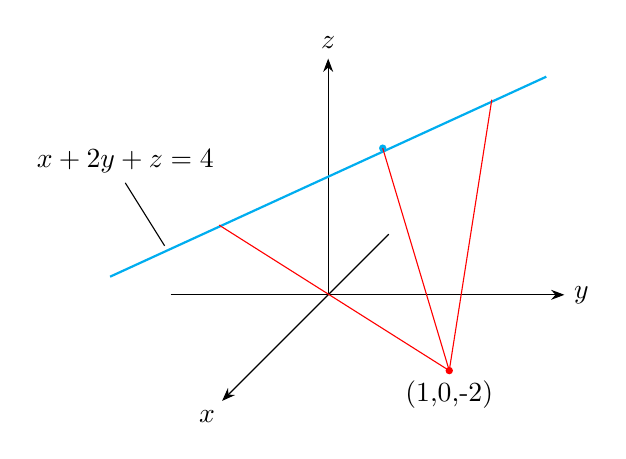
\begin{tikzpicture}[=>stealth]
\draw[-Stealth](-2,0,0)--(3,0,0)node[right]{$y$};
\draw[-Stealth](0,0,0)--(0,3,0)node[above]{$z$};
\draw[-Stealth](0,0,-2)--(0,0,3.5);
\draw(0,0,4)node[]{$x$}
(2.5,0,2.5)node[below]{(1,0,-2)};
\draw[cyan,thick](-2,1,2)--(2,2,-2)
(0.5,1.67,-0.5)node[shape=circle,scale=0.01cm,fill=cyan]{};
\draw[red]
(2.5,0,2.5)node[shape = circle, scale = 0.01cm, fill=red]{}
(2.5,0,2.5)--(-1,1.27,1)
(2.5,0,2.5)--(1.5,1.9,-1.5)
(2.5,0,2.5)--(0.5,1.67,-0.5);
\draw(-2,2,1.5)--(-1.5,1.2,1.5)
(-2,2,1.5)node[above]{$x + 2y + z = 4$};
\end{tikzpicture}
\end{figure}
\end{solution}

\begin{exa}
\label{ex:degenerate}
Show that the second derivative test fails at the origin for both
$f(x,y) = x^4 + y^4$ and $g(x,y) = x^4 - y^4$, and classify the origin for each.
\end{exa}

\begin{solution}
All first and second partial derivatives of both functions vanish at the origin,
so $D = 0$ for each and the test is silent. Directly: $f(x,y)>0 = f(0,0)$ for
$(x,y)\neq(0,0)$, so $f$ has an absolute minimum at the origin, while
$g(x,0) = x^4>0$ and $g(0,y) = -y^4<0$, so $g$ has a saddle point. Two functions
with the same second derivatives at a point can behave differently there, which
is why $D = 0$ must be reported as inconclusive.
\end{solution}

\begin{exa}
\label{ex:cubicsaddles}
Find and classify the critical points of $f(x,y) = x^3 - 3x + y^2 - 4y$.
\end{exa}

\begin{solution}
$f_x = 3x^2 - 3 = 0$ gives $x = \pm1$, and $f_y = 2y - 4 = 0$ gives $y = 2$. With
$f_{xx} = 6x$, $f_{yy} = 2$ and $f_{xy} = 0$, $D = 12x$.
\begin{enumerate}
\item[$-$] At $(1,2)$: $D = 12>0$ and $f_{xx} = 6>0$, a local minimum, with
$f(1,2) = 1 - 3 + 4 - 8 = -6$.
\item[$-$] At $(-1,2)$: $D = -12<0$, a saddle point, with
$f(-1,2) = -1 + 3 + 4 - 8 = -2$.
\end{enumerate}
The local minimum is not absolute: $f(x,2) = x^3 - 3x - 4\to -\infty$ as
$x\to -\infty$.
\end{solution}

{\color[wave]{485}\subsection{Extrema for Functions with Side Conditions (Constraints)}}

\subhead{Lagrange Multipliers}

Often a function is to be maximised or minimised not over a region but along a
curve or surface: the largest volume for a given surface area, the hottest point
on a wire. Consider the problem of finding the extreme values of $f(x,y)$
subject to the constraint $g(x,y) = k$. To maximise $f$ is to find the largest
value $c$ for which the level curve $f(x,y) = c$ still meets the curve
$g(x,y) = k$. At that value the two curves touch without crossing: they have a
common tangent line at the point of contact.

\begin{figure}[H]
\centering
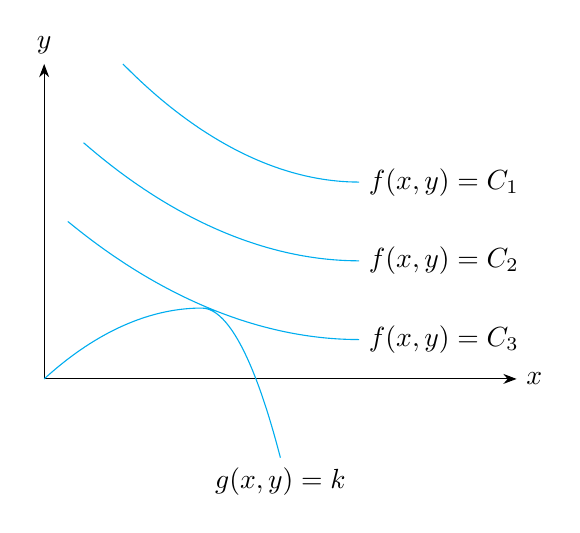
\begin{tikzpicture}[=>stealth]
\draw[-Stealth](0,0)--(6,0)node[right]{$x$};
\draw[-Stealth](0,0)--(0,4)node[above]{$y$};
\draw[cyan](1,4)parabola[bend at end](4,2.5)node[right,black]{$f(x,y)=C_1$}
(0.5,3)parabola[bend at end](4,1.5)node[right,black]{$f(x,y)=C_2$}
(0.3,2)parabola[bend at end](4,0.5)node[right,black]{$f(x,y)=C_3$}
(0,0)parabola[bend at end](2,0.9)
(2,0.9)parabola(3,-1)node[below,black]{$g(x,y)=k$};
\end{tikzpicture}
\end{figure}

Their normal lines at the point $(x_0,y_0)$ then coincide, and since gradients
are normal to level curves, the gradient vectors are parallel:
\[ \nabla f(x_0,y_0) = \lambda \nabla g(x_0,y_0)\]
for some scalar $\lambda$, called a \emph{Lagrange multiplier}. The argument is
made precise by the following theorem.

\begin{thm}[Lagrange]
\label{thm:lagrange}
Let $f$ and $g$ have continuous first partial derivatives, and suppose that $f$,
restricted to the curve $g(x,y) = k$, has a local maximum or minimum at
$(x_0,y_0)$, where $\nabla g(x_0,y_0)\neq\mathbf 0$. Then there is a number
$\lambda$ with $\nabla f(x_0,y_0) = \lambda\nabla g(x_0,y_0)$. The same holds
for $f(x,y,z)$ restricted to a surface $g(x,y,z) = k$.
\end{thm}

\begin{proof}
Since $\nabla g(x_0,y_0)\neq\mathbf 0$, the implicit function theorem (the
subsection of that name) shows that near $(x_0,y_0)$ the curve $g = k$ is the
path of a differentiable curve $\mathbf r(t)$ with $\mathbf r(0) = (x_0,y_0)$
and $\mathbf r'(0)\neq\mathbf 0$. The function $t\mapsto f(\mathbf r(t))$ has a
local extremum at $t = 0$, so its derivative $\nabla f\cdot\mathbf r'(0)$ is
zero there. Also $g(\mathbf r(t)) = k$ for all $t$, so
$\nabla g\cdot\mathbf r'(0) = 0$. In the plane, both $\nabla f$ and $\nabla g$
are therefore perpendicular to the same non-zero vector $\mathbf r'(0)$, hence
parallel, and since $\nabla g\neq\mathbf 0$, $\nabla f = \lambda\nabla g$. On a
surface the same reasoning applies to every curve through $(x_0,y_0,z_0)$ in the
surface, so $\nabla f$ is perpendicular to the whole tangent plane, as $\nabla g$
is.
\end{proof}

\subhead{Method of Lagrange Multipliers}

To find the maximum and minimum values of $f(x,y,z)$ subject to the constraint
$g(x,y,z) = k$, assuming that these extreme values exist and that
$\nabla g \neq \mathbf 0$ on the surface $g(x,y,z) = k$:
\begin{enumerate}
\item Find all values of $x$, $y$, $z$ and $\lambda$ such that
\[\nabla f(x,y,z) = \lambda \nabla g(x,y,z)\qquad\text{and}\qquad g(x,y,z) =
k .\]

\item Evaluate $f$ at all the points $(x,y,z)$ found in step 1. The largest of
these values is the maximum of $f$, and the smallest is the minimum.
\end{enumerate}
In components, step 1 is a system of four equations, $f_x = \lambda g_x$,
$f_y = \lambda g_y$, $f_z = \lambda g_z$ and $g = k$, in four unknowns. For a
function of two variables there are three equations in $x$, $y$ and $\lambda$.

\begin{exa}
\label{ex:lagrangeline}
Find the extreme values of $f(x,y) = x + y$ subject to the constraint
$x^2 + y^2 = 1$.

\begin{figure}[H]
\centering
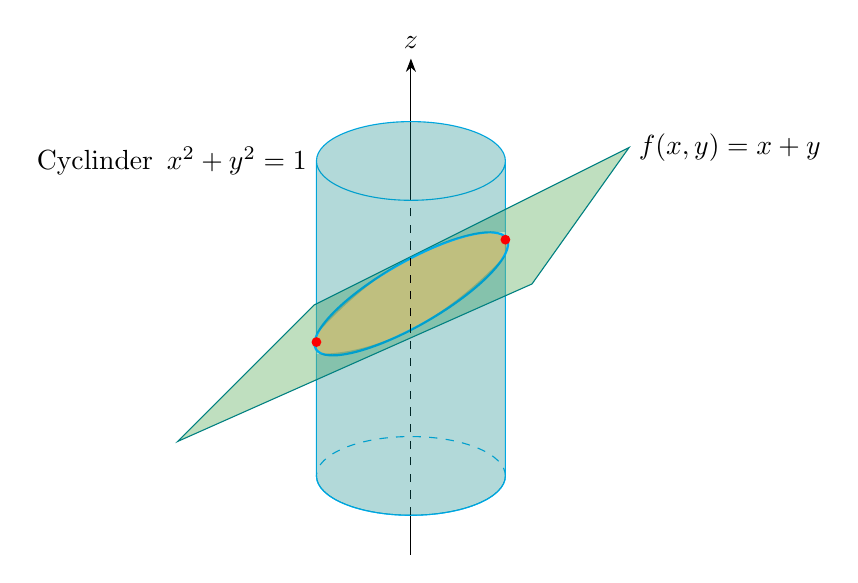
\begin{tikzpicture}[=>stealth]
%\draw[-Stealth](-2,0,0)--(2,0,0)node[right]{$y$};
\draw[-Stealth](0,3.5,0)--(0,5.3,0)node[above]{$z$};
%\draw[-Stealth](0,0,-2)--(0,0,3);
%\draw(0,0,3.5)node[]{$x$};
\draw[cyan](-1.2,0)arc(180:360:1.2cm and 0.5cm)
(1.2,0)--(1.2,4)
(-1.2,0)--(-1.2,4)
(1.2,4)arc(0:360:1.2cm and 0.5cm);
\path[fill=orange,opacity=0.5, rotate=30](2.56,2)arc(0:360:1.4cm and 0.4cm);
\path[fill=orange!50!cyan,opacity=0.5](-2,1.4,2.5)--(2.5,3.4,2.5)--(2,3.4,-2)--(-2,1.4,-2)--cycle;
\draw[teal](-2,1.4,2.5)--(2.5,3.4,2.5)--(2,3.4,-2)--(-2,1.4,-2)--cycle;
%%%
\draw(0,-1)--(0,-0.45)
(2,3.4,-2)node[right]{$f(x,y)=x +y$}
(-1.2,4)node[left]{Cyclinder $\, x^2 + y^2 = 1$};
%\shade[right color=teal,opacity=0.1](1.2,4)arc(0:360:1.2cm and 0.5cm);
\draw[cyan](-1.2,0)arc(180:360:1.2cm and 0.5cm);
\draw[rotate=30,thick,cyan](2.56,2)arc(0:360:1.4cm and 0.4cm);
\draw[dashed,cyan](1.2,0)arc(0:180:1.2cm and 0.5cm);
\draw[dashed](0,-0.5)--(0,3.4);
\draw(1.2,3)node[shape=circle,fill=red,draw=red,thick,scale=0.01cm]{}
(-1.2,1.7)node[shape=circle,fill=red,draw=red,thick,scale=0.01cm]{};
\path[fill=teal,opacity=0.3](-1.2,1.8)--(-1.2,0)--(-1.2,0)arc(180:360:1.2cm and 0.5cm)--(1.2,0)--(1.2,3)--(1.2,2.8)parabola[bend at end](-1.2,1.55)--(-1.2,1.8);
\path[fill=teal,opacity=0.3](1.2,3)--(1.2,4)--(1.2,4)arc(0:180:1.2cm and 0.5cm)--(-1.2,4)--(-1.2,1.8)--(-1.2,1.8)parabola[bend at end](1.2,3.1)--cycle;
\end{tikzpicture}
\end{figure}

Geometrically, the graph of $f$ is the plane $z = x + y$ and the constraint is
the cylinder $x^2 + y^2 = 1$; the problem asks for the highest and lowest points
of the ellipse in which they meet. In the plane, the level curves $x + y = k$
are parallel lines, and the extreme values of $k$ are those for which the line
just touches the unit circle.

\begin{figure}[H]
\centering
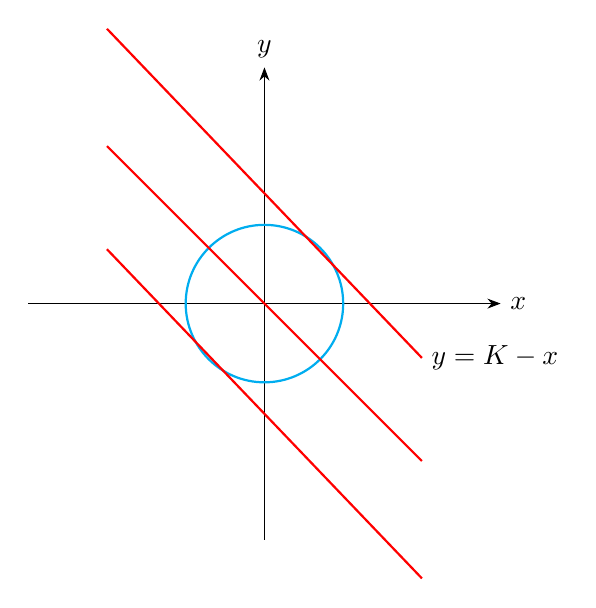
\begin{tikzpicture}[=>stealth]
\draw[-Stealth](-3,0)--(3,0)node[right]{$x$};
\draw[-Stealth](0,-3)--(0,3)node[above]{$y$};
\draw[thick,cyan](0,0)circle [radius=1cm];
\draw[thick,red](-2,2)--(2,-2);
\draw[thick,red](-2,3.49)--(2,-0.69);
\draw[thick,red](-2,0.69)--(2,-3.49);
\draw(2,-0.69)node[right]{$y = K - x$};
\end{tikzpicture}
\end{figure}

With $g(x,y) = x^2 + y^2$, $\nabla f = \langle 1, 1\rangle$ and
$\nabla g = \langle 2x, 2y\rangle$, so the equations are
\[1 = 2\lambda x,\qquad 1 = 2\lambda y,\qquad x^2 + y^2 = 1 .\]
The first two show $\lambda\neq 0$ and $x = y = \frac{1}{2\lambda}$. Then
$2x^2 = 1$, so $x = y = \pm \frac{\sqrt{2}}{2}$, giving the candidates
$\left(\frac{\sqrt{2}}{2}, \frac{\sqrt{2}}{2}\right)$ and
$\left(-\frac{\sqrt{2}}{2}, -\frac{\sqrt{2}}{2}\right)$. There
\[f\left(\frac{\sqrt{2}}{2}, \frac{\sqrt{2}}{2}\right)=\sqrt{2}\ \ \text{(the
maximum)},\qquad f\left(-\frac{\sqrt{2}}{2}, -\frac{\sqrt{2}}{2}\right)=-\sqrt{2}
\ \ \text{(the minimum)}.\]

\begin{figure}[H]
\centering
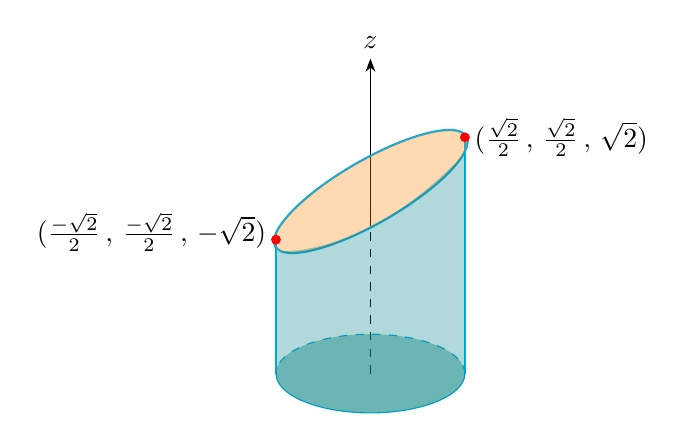
\begin{tikzpicture}[=>stealth]
%\draw[-Stealth](1.2,0,0)--(2.3,0,0)node[right]{$y$};
\draw[-Stealth](0,1.87,0)--(0,4,0)node[above]{$z$};
%\draw[-Stealth](0,0,1.2)--(0,0,3);
\draw[cyan](-1.2,0)arc(180:360:1.2cm and 0.5cm);
\draw[cyan](1.2,0)--(1.2,3)
(-1.2,0)--(-1.2,1.8);
\draw[rotate=30,thick,cyan](2.56,2)arc(0:360:1.4cm and 0.4cm);
\path[fill=orange,opacity=0.3, rotate=30](2.56,2)arc(0:360:1.4cm and 0.4cm);
\draw[dashed,cyan](1.2,0)arc(0:180:1.2cm and 0.5cm);
\draw[dashed](0,0)--(0,1.8);
\draw(1.2,3)node[shape=circle,fill=red,draw=red,thick,scale=0.01cm]{}
(-1.2,1.7)node[shape=circle,fill=red,draw=red,thick,scale=0.01cm]{}
(1.2,3)node[right]{$(\frac{\sqrt{2}}{2}\, ,\, \frac{\sqrt{2}}{2}\, ,\, \sqrt{2})$}
(-1.2,1.8)node[left]{$(\frac{- \sqrt{2}}{2}\, ,\, \frac{-\sqrt{2}}{2}\, ,\, -\sqrt{2})$};
\path[fill=teal,opacity=0.4](1.2,0)arc(0:360:1.2cm and 0.5cm);
\path[fill=teal,opacity=0.3](-1.2,1.8)--(-1.2,0)--(-1.2,0)arc(180:360:1.2cm and 0.5cm)--(1.2,0)--(1.2,3)--(1.2,2.8)parabola[bend at end](-1.2,1.55)--(-1.2,1.8);
\end{tikzpicture}
\end{figure}
\end{exa}

\begin{exa}
\label{ex:lagrangeellipse}
Find the extreme values of the function $f(x,y) = x^2 + 2y^2$ on the circle
$x^2 + y^2 = 1$.

With $g(x,y) = x^2 + y^2$, the equations $\nabla f = \lambda\nabla g$ and the
constraint read
\[2x = 2\lambda x,\qquad 4y = 2\lambda y,\qquad x^2 + y^2 = 1 .\]
The first gives $x = 0$ or $\lambda = 1$.
\begin{enumerate}
\item[$-$] If $x = 0$, the constraint gives $y = \pm 1$.
\item[$-$] If $\lambda = 1$, the second equation becomes $4y = 2y$, so $y = 0$,
and the constraint gives $x = \pm 1$.
\end{enumerate}
The candidates are $(0,\pm1)$ and $(\pm1,0)$, where
\[f(0,\pm1) = 2,\qquad f(\pm1,0) = 1 .\]
So the maximum of $f$ on the circle is $2$, at $(0,\pm 1)$, and the minimum is
$1$, at $(\pm 1, 0)$. Geometrically, the circle lies on the paraboloid
$z = x^2 + 2y^2$ along a closed curve whose highest points lie over the
$y$-axis and lowest over the $x$-axis.

\begin{figure}[H]
\centering
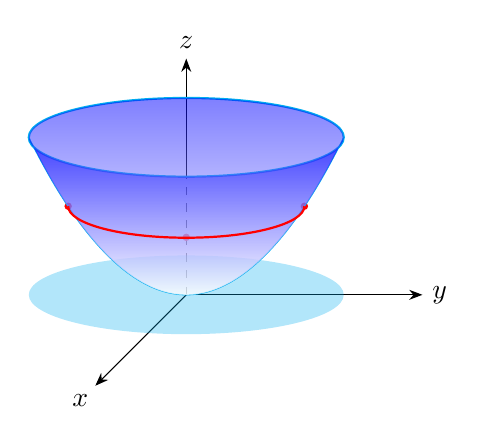
\begin{tikzpicture}[=>stealth]
\draw[-Stealth](0,0,0)--(3,0,0)node[right]{$y$};
\draw[-Stealth](0,1.5,0)--(0,3,0)node[above]{$z$};
\draw[-Stealth](0,0,0)--(0,0,3);
\draw[dashed](0,0,0)--(0,1.5,0);
\draw(0,0,3.5)node[]{$x$}
(-1.5,1.125)node[shape=circle,fill=red,scale=0.01cm]{}
(0,0.73)node[shape=circle,fill=red,scale=0.01cm]{}
(1.5,1.125)node[shape=circle,fill=red,scale=0.01cm]{};
\path[fill=cyan,opacity=0.3](0,0)circle(2cm and 0.5cm);
\draw[cyan](0,0) parabola(2,2)
(0,0)parabola(-2,2);
\draw[thick,cyan](0,2)ellipse[x radius = 2cm , y radius = 0.5cm];
\shade[top color=blue,opacity=0.5](0,0)parabola(-2,2)--(-2,2)arc(180:0:2cm and 0.5cm)--(2,2)parabola[bend at end](0,0);
\shade[top color=blue,opacity=0.6](0,0)parabola(-2,2)--(-2,2)arc(180:360:2cm and 0.5cm)--(2,2)parabola[bend at end](0,0)--cycle;
\draw[thick,red](-1.5,1.125)arc(180:360:1.5cm and 0.4cm);
\end{tikzpicture}
\end{figure}
\end{exa}

\subhead{Two Constraints}

To find the extreme values of $f(x,y,z)$ subject to two constraints
\[g(x,y,z) = k,\qquad h(x,y,z) = c ,\]
whose intersection is a curve, the same reasoning shows that at an extreme
point $\nabla f$ lies in the plane spanned by $\nabla g$ and $\nabla h$
(provided these are not parallel):
\[\nabla f =\lambda \nabla g + \mu \nabla h .\]
In components this gives five equations in the five unknowns $x$, $y$, $z$,
$\lambda$ and $\mu$:
\[f_x = \lambda g_x + \mu h_x,\quad f_y = \lambda g_y + \mu h_y,\quad f_z =
\lambda g_z + \mu h_z,\quad g = k,\quad h = c .\]

\begin{exa}
\label{ex:twoconstraints}
Find the maximum value of the function $f(x,y,z) = x + 2y + 3z$ on the curve of
intersection of the plane $x - y + z =1$ and the cylinder $x^2 + y^2 = 1$.
\end{exa}

\begin{solution}
With $g = x - y + z$ and $h = x^2 + y^2$,
\[\nabla f = \langle 1, 2, 3\rangle,\qquad \nabla g = \langle 1, -1,
1\rangle,\qquad \nabla h = \langle 2x, 2y, 0\rangle ,\]
so the equations are
\begin{align}
1 & = \lambda + 2\mu x, \label{eq:tc1}\\
2 & = -\lambda + 2\mu y, \label{eq:tc2}\\
3 & = \lambda, \label{eq:tc3}\\
x - y + z & = 1, \label{eq:tc4}\\
x^2 + y^2 & = 1 . \label{eq:tc5}
\end{align}
By \eqref{eq:tc3}, $\lambda = 3$, and then \eqref{eq:tc1} and \eqref{eq:tc2}
give
\[2\mu x = -2,\qquad 2\mu y = 5,\qquad\text{so}\qquad x = -\frac{1}{\mu},\quad
y = \frac{5}{2\mu}.\]
Substituting into \eqref{eq:tc5},
\[\frac{1}{\mu^2}+ \frac{25}{4\mu^2} = 1 ,\qquad \mu^2 = \frac{29}{4},\qquad \mu =
\pm\frac{\sqrt{29}}{2},\]
so $x = \mp \frac{2}{\sqrt{29}}$ and $y = \pm \frac{5}{\sqrt{29}}$, with the
signs taken together. From \eqref{eq:tc4},
$z = 1 - x + y = 1 \pm \frac{7}{\sqrt{29}}$. The two candidates are
\[\left(-\frac{2}{\sqrt{29}}, \frac{5}{\sqrt{29}}, 1 + \frac{7}{\sqrt{29}}\right)
\quad\text{and}\quad \left(\frac{2}{\sqrt{29}}, -\frac{5}{\sqrt{29}}, 1 -
\frac{7}{\sqrt{29}}\right),\]
where
\[f = 3 \pm\frac{-2 + 10 + 21}{\sqrt{29}} = 3 \pm \frac{29}{\sqrt{29}} = 3\pm
\sqrt{29} .\]
The maximum value is $3 + \sqrt{29}\approx 8.39$, and the minimum is
$3 - \sqrt{29}$.
\end{solution}

\begin{exa}
\label{ex:cheapestbox}
A closed rectangular box is to have volume $32\ \text{m}^3$. The base costs
twice as much per square metre as the top and sides. Find the dimensions that
minimise the cost.
\end{exa}

\begin{solution}
Let the base be $x$ by $y$ and the height $z$, and measure cost in units of the
price of the top and sides per square metre. The cost is
$C = 2xy + xy + 2xz + 2yz = 3xy + 2xz + 2yz$, to be minimised subject to
$xyz = 32$. The Lagrange equations are
\[3y + 2z = \lambda yz,\qquad 3x + 2z = \lambda xz,\qquad 2x + 2y = \lambda xy .\]
Multiplying the first by $x$ and the second by $y$ and subtracting gives
$2z(x - y) = 0$, so $x = y$. Multiplying the second by $y$ and the third by $z$
and subtracting gives $3xy - 2yz = 0$ (using $x = y$), so $z = \frac32 x$. Then
$xyz = \frac32 x^3 = 32$, so $x^3 = \frac{64}{3}$ and
\[x = y = \frac{4}{\sqrt[3]{3}}\approx 2.77\ \text{m},\qquad z = \frac32 x\approx
4.16\ \text{m}.\]
The more expensive base makes the box taller than a cube.
\end{solution}

\begin{exa}
\label{ex:entropy}
Find the maximum of $f(x,y,z) = xyz$ for positive $x$, $y$, $z$ with
$x + y + z = 12$, and deduce the inequality of arithmetic and geometric means
for three numbers.
\end{exa}

\begin{solution}
The equations $yz = \lambda$, $xz = \lambda$, $xy = \lambda$ give
$yz = xz = xy$, and since the variables are positive, $x = y = z$. The constraint
then gives $x = y = z = 4$ and the maximum $f = 64$. (The maximum exists because
$f$ is continuous on the closed bounded triangle $x,y,z\geq 0$, $x+y+z = 12$ and
vanishes on its edges.) Replacing $12$ by any sum $s$ gives the maximum
$\left(\frac{s}{3}\right)^3$, so for positive numbers with sum $s$,
\[xyz\leq\left(\frac{x+y+z}{3}\right)^3,\qquad\text{that is}\qquad \sqrt[3]{xyz}
\leq\frac{x+y+z}{3},\]
with equality only when $x = y = z$.
\end{solution}

{\color[wave]{485}\subsection{Absolute Maximum and Minimum Values}}

For a function of one variable, a continuous function on a closed interval
attains a maximum and a minimum. The analogue in the plane replaces the closed
interval by a set that is closed (it contains all its boundary points) and
bounded (it lies inside some disc).

\begin{thm}[Extreme value theorem]
\label{thm:evt}
If $f$ is continuous on a closed bounded set $D$ in $\mathbb{R}^2$, then $f$
attains an absolute maximum value $f(x_1,y_1)$ and an absolute minimum value
$f(x_2,y_2)$ at some points $(x_1,y_1)$ and $(x_2,y_2)$ of $D$.
\end{thm}

An extreme value attained at an interior point of $D$ is also a local extreme
value, so by Theorem~\ref{thm:fermat} it occurs at a critical point. Every other
extreme value is attained on the boundary. This gives a procedure.

\subhead{Closed Interval Method}
To find the absolute maximum and minimum of a continuous function $f$ on a
closed bounded set $D$:
\begin{enumerate}
\item Find the values of $f$ at the critical points of $f$ in the interior of
$D$.

\item Find the extreme values of $f$ on the boundary of $D$.

\item The largest of the values from steps 1 and 2 is the absolute maximum
value, and the smallest is the absolute minimum value.
\end{enumerate}
Step 2 usually reduces to one-variable problems, one for each piece of the
boundary, or is done with Lagrange multipliers.

\begin{exa}
\label{ex:rectangle}
Find the absolute maximum and minimum values of $f(x,y) = x^2 - 2xy + 2y$ on the
rectangle $D = \{(x,y) \mid 0\leq x \leq 3,\ 0 \leq y \leq 2 \}$.
\end{exa}

\begin{solution}
The polynomial $f$ is continuous on the closed bounded rectangle, so the
extreme values exist.

\emph{Interior.} $f_x = 2x -2y$ and $f_y = -2x + 2$ vanish only at $(1,1)$, which
lies inside $D$, and $f(1,1) = 1$.

\emph{Boundary.} The boundary consists of the four segments $L_1$ to $L_4$.

\begin{figure}[H]
\centering
\begin{tikzpicture}[=>stealth]
\draw[-Stealth](0,0)--(4,0)node[right]{$x$};
\draw[-Stealth](0,0)--(0,3)node[above]{$y$};
\draw[cyan](0,0)rectangle(3,2);
\draw(0,0)node[below]{$0$}
(3,0)node[below]{$3$}
(3,2)node[right]{$(3,2)$}
(0,2)node[left]{$2$}
(1.5,0)node[below,scale=0.9]{$L_1$}
(3,1)node[right,scale=0.9]{$L_2$}
(1.5,2)node[above,scale=0.9]{$L_3$}
(0,1)node[left,scale=0.9]{$L_4$};
\end{tikzpicture}
\end{figure}

\begin{enumerate}
\item[$-$] On $L_1$: $y = 0$, $0\leq x\leq 3$, and $f = x^2$, which increases from
$0$ to $9$.
\item[$-$] On $L_2$: $x = 3$, $0\leq y\leq 2$, and $f = 9 - 4y$, which decreases
from $9$ to $1$.
\item[$-$] On $L_3$: $y = 2$, $0\leq x\leq 3$, and $f = x^2 - 4x + 4 = (x-2)^2$,
with minimum $0$ at $x = 2$ and maximum $4$ at $x = 0$.
\item[$-$] On $L_4$: $x = 0$, $0\leq y\leq 2$, and $f = 2y$, from $0$ to $4$.
\end{enumerate}

\emph{Comparison.} The candidates are $1$ from the interior and $0$, $1$, $4$, $9$
from the boundary. The absolute maximum is $f(3,0) = 9$, and the absolute minimum
is $0$, attained at $(0,0)$ and at $(2,2)$.
\end{solution}

\begin{exa}
\label{ex:triangle}
Find the absolute extreme values of $f(x,y) = x^2 + y^2 - 2x - 2y$ on the closed
triangle with vertices $(0,0)$, $(4,0)$ and $(0,4)$.
\end{exa}

\begin{solution}
\emph{Interior.} $f_x = 2x - 2 = 0$ and $f_y = 2y - 2 = 0$ give $(1,1)$, inside the
triangle, with $f(1,1) = -2$.

\emph{Boundary.} On $y = 0$, $0\leq x\leq 4$: $f = x^2 - 2x$, with minimum $-1$ at
$x = 1$ and values $0$ and $8$ at the ends. On $x = 0$ the same by symmetry. On
the hypotenuse $y = 4 - x$, $0\leq x\leq 4$:
\[f = x^2 + (4-x)^2 - 2x - 2(4-x) = 2x^2 - 8x + 8 = 2(x-2)^2,\]
with minimum $0$ at $(2,2)$ and maximum $8$ at the ends.

\emph{Comparison.} The absolute minimum is $-2$ at $(1,1)$, and the absolute
maximum is $8$, at $(4,0)$ and $(0,4)$.
\end{solution}

\begin{exa}
\label{ex:discboundary}
Find the absolute extreme values of $f(x,y) = 2x^2 + y^2 - 4x + 1$ on the disc
$x^2 + y^2\leq 4$, using a Lagrange multiplier on the boundary.
\end{exa}

\begin{solution}
\emph{Interior.} $f_x = 4x - 4$ and $f_y = 2y$ vanish at $(1,0)$, inside the disc,
where $f = -1$.

\emph{Boundary.} On $x^2 + y^2 = 4$, the equations $\nabla f = \lambda\nabla g$
are $4x - 4 = 2\lambda x$ and $2y = 2\lambda y$. The second gives $y = 0$ or
$\lambda = 1$. If $y = 0$, then $x = \pm 2$, with $f(2,0) = 1$ and
$f(-2,0) = 17$. If $\lambda = 1$, the first gives $4x - 4 = 2x$, so $x = 2$ and
$y = 0$ again.

\emph{Comparison.} The absolute maximum is $17$, at $(-2,0)$, and the absolute
minimum is $-1$, at $(1,0)$.
\end{solution}


{\color[wave]{485}\subsection{Taylor's Formula For Functions of Several Variables}}

For a function of one variable with $n+1$ continuous derivatives, Taylor's
theorem gives
\[f(a+h) = f(a) + f'(a)\,h + \frac{f''(a)}{2!}h^2 + \cdots + \frac{f^{(n)}(a)}{n!}h^n
+ R_n,\qquad R_n = \frac{f^{(n+1)}(a+\theta h)}{(n+1)!}h^{n+1}\]
for some $\theta$ between $0$ and $1$. The two-variable version is obtained by
applying this along a line, and it is most compactly written with the operator
\[h\frac{\partial}{\partial x} + k\frac{\partial}{\partial y},\qquad\text{so that}
\qquad \left(h\frac{\partial}{\partial x} + k\frac{\partial}{\partial y}\right)f =
hf_x + kf_y ,\]
and its powers are expanded by the binomial theorem, for example
\[\left(h\frac{\partial}{\partial x} + k\frac{\partial}{\partial y}\right)^2f =
h^2f_{xx} + 2hkf_{xy} + k^2f_{yy} .\]

\begin{thm}[Taylor's formula]
\label{thm:taylor2}
Suppose $f(x,y)$ and its partial derivatives up to order $n+1$ are continuous on
an open set containing the segment from $(a,b)$ to $(a+h,b+k)$. Then
\[f(a+h,b+k) = \sum_{m=0}^{n}\frac{1}{m!}\left(h\frac{\partial}{\partial x} +
k\frac{\partial}{\partial y}\right)^m f(a,b) + R_n ,\]
where
$R_n = \frac{1}{(n+1)!}\left(h\frac{\partial}{\partial x} +
k\frac{\partial}{\partial y}\right)^{n+1}f(a+\theta h,b+\theta k)$ for some
$\theta$ with $0<\theta<1$.
\end{thm}

\begin{proof}
Let $g(t) = f(a+th,b+tk)$ for $0\leq t\leq 1$. By the chain rule,
$g'(t) = hf_x + kf_y$ evaluated at $(a+th,b+tk)$, and applying it again to each
term, $g^{(m)}(t) = \left(h\frac{\partial}{\partial x} +
k\frac{\partial}{\partial y}\right)^m f(a+th,b+tk)$; the mixed derivatives can be
collected because $f_{xy} = f_{yx}$ for functions with continuous second
derivatives. The one-variable formula for $g$ with $a = 0$ and step $1$,
\[g(1) = g(0) + g'(0) + \frac{g''(0)}{2!} + \cdots + \frac{g^{(n)}(0)}{n!} +
\frac{g^{(n+1)}(\theta)}{(n+1)!},\]
is exactly the statement, since $g(1) = f(a+h,b+k)$.
\end{proof}

With $n = 0$ the theorem reads
$f(a+h,b+k) = f(a,b) + hf_x(a+\theta h, b+\theta k) + kf_y(a+\theta h,b+\theta
k)$, the \emph{mean value theorem} for functions of two variables. Taking
$a = b = 0$, $h = x$ and $k = y$ gives the expansion in powers of $x$ and $y$ (the
Maclaurin expansion):
\begin{align*}
f(x,y) = {} & f(0,0) + \big(xf_x + yf_y\big) + \frac{1}{2!}\big(x^2f_{xx} + 2xyf_{xy} +
y^2f_{yy}\big)\\
& + \frac{1}{3!}\big(x^3f_{xxx} + 3x^2y f_{xxy} + 3xy^2f_{xyy} + y^3f_{yyy}\big)
+\cdots ,
\end{align*}
with every derivative evaluated at $(0,0)$.

\begin{exa}
\label{ex:taylorexpsin}
Expand $f(x,y) = e^x \sin y$ about $(0,0)$ in powers of $x$ and $y$ up to terms of
the third degree.
\end{exa}

\begin{solution}
Each derivative is $e^x$ times a derivative of $\sin y$, so
\begin{align*}
& f = e^x\sin y \to 0, && f_x = e^x\sin y \to 0, && f_y = e^x\cos y \to 1,\\
& f_{xx} = e^x\sin y \to 0, && f_{xy} = e^x\cos y \to 1, && f_{yy} = -e^x\sin y
\to 0,\\
& f_{xxx} = e^x\sin y \to 0, && f_{xxy} = e^x\cos y \to 1, && f_{xyy} = -e^x\sin y
\to 0,\\
& f_{yyy} = -e^x\cos y \to -1,
\end{align*}
the arrows giving the values at $(0,0)$. By Theorem~\ref{thm:taylor2},
\[e^x\sin y = y + \frac{1}{2!}(2xy) + \frac{1}{3!}(3x^2y - y^3) + \cdots = y + xy
+ \frac{x^2y}{2} - \frac{y^3}{6} + \cdots .\]
As a check, multiplying the series $e^x = 1 + x + \frac{x^2}{2}+\cdots$ and
$\sin y = y - \frac{y^3}{6}+\cdots$ and keeping terms of degree at most three
gives the same result.
\end{solution}

\begin{exa}
\label{ex:taylorpoly}
Expand $f(x,y) = x^2y + 3y -2$ in powers of $x - 1$ and $y + 2$.
\end{exa}

\begin{solution}
The point is $(a,b) = (1,-2)$, where $f(1,-2) = -2 - 6 - 2 = -10$. The
derivatives and their values there are
\begin{align*}
& f_x = 2xy \to -4, && f_y = x^2 + 3 \to 4,\\
& f_{xx} = 2y \to -4, && f_{xy} = 2x \to 2, && f_{yy} = 0,\\
& f_{xxy} = 2, && f_{xxx} = f_{xyy} = f_{yyy} = 0 ,
\end{align*}
and all higher derivatives vanish, so the expansion terminates. With $h = x - 1$
and $k = y + 2$,
\begin{align*}
f(x,y) & = -10 - 4h + 4k + \frac{1}{2!}\left(-4h^2 + 2\cdot 2hk\right) +
\frac{1}{3!}\left(3h^2k\cdot 2\right)\\
& = -10 - 4(x-1) + 4(y+2) - 2(x-1)^2 + 2(x-1)(y+2) + (x-1)^2(y+2) .
\end{align*}
This is exact, since $f$ is a polynomial of degree three; substituting
$x = 1 + h$, $y = -2 + k$ directly gives the same result.
\end{solution}

\begin{exe}
\label{exe:coscos}
Find the expansion of $\cos x \cos y$ in powers of $x$ and $y$ up to terms of the
fourth order.

\textbf{Answer:}
$\cos x\cos y = 1 - \frac{x^2}{2}-\frac{y^2}{2} + \frac{x^4}{24} +
\frac{x^2y^2}{4} + \frac{y^4}{24}+\cdots$, most easily found by multiplying the
two one-variable series.
\end{exe}

\begin{exa}
\label{ex:taylorestimate}
Use the second-degree Taylor polynomial of $f(x,y) = \sqrt{x^2 + y^3}$ about
$(1,2)$ to estimate $f(1.02, 1.97)$.
\end{exa}

\begin{solution}
At $(1,2)$, $s = x^2 + y^3 = 9$ and $f = 3$. With $f = s^{1/2}$,
\[f_x = \frac{x}{\sqrt s} = \frac13,\qquad f_y = \frac{3y^2}{2\sqrt s} = 2,\]
\[f_{xx} = \frac{1}{\sqrt s} - \frac{x^2}{s^{3/2}} = \frac13 - \frac1{27} =
\frac{8}{27},\qquad f_{xy} = -\frac{3xy^2}{2s^{3/2}} = -\frac{2}{9},\qquad
f_{yy} = \frac{3y}{\sqrt s} - \frac{9y^4}{4s^{3/2}} = 2 - \frac43 = \frac23 .\]
With $h = 0.02$ and $k = -0.03$,
\[f\approx 3 + \frac{0.02}{3} - 0.06 + \frac12\left(\frac{8}{27}(0.0004) -
\frac{4}{9}(-0.0006) + \frac23(0.0009)\right)\approx 2.94716 .\]
The exact value is $\sqrt{1.0404 + 7.645373} = 2.94716$ to five decimal places.
The linear approximation alone gives $2.94667$; the quadratic terms recover
almost all of the difference.
\end{solution}

\begin{exa}
\label{ex:taylorclassify}
Use a second-degree expansion to classify the critical point at the origin of
$f(x,y) = e^{xy} - \cos(x+y)$.
\end{exa}

\begin{solution}
From the one-variable series,
$e^{xy} = 1 + xy + \cdots$ and $\cos(x+y) = 1 - \frac{(x+y)^2}{2} + \cdots$,
where the omitted terms have degree at least $4$ in the first case and at
least $4$ in the second. So
\[f(x,y) = xy + \frac{(x+y)^2}{2} + \cdots = \frac{x^2}{2} + 2xy +
\frac{y^2}{2} + \cdots .\]
There are no linear terms, so the origin is a critical point, and comparing with
Theorem~\ref{thm:taylor2}, $f_{xx} = 1$, $f_{xy} = 2$, $f_{yy} = 1$ there. Then
$D = 1 - 4 = -3<0$, and the origin is a saddle point. Along $y = x$ the quadratic
part is $3x^2>0$, and along $y = -x$ it is $-x^2<0$.
\end{solution}

{\color[wave]{485}\subsection{Composite Functions and Chain Rule Differentiation}}

Let $z = f(x,y)$, where $x = g(r,s)$ and $y = h(r,s)$, so that $z$ is a function
of $r$ and $s$. The chain rule expresses the derivatives of $z$ with respect to
the new variables through those with respect to the old.

\begin{thm}[Chain rule]
\label{thm:chain}
Suppose $f$ is differentiable at $(x,y)$, where $x = g(r,s)$ and $y = h(r,s)$, and
$g$ and $h$ have partial derivatives at $(r,s)$. Then
\[\frac{\partial z}{\partial r} =\frac{\partial z}{\partial x}
\frac{\partial x}{\partial r} + \frac{\partial z}{\partial y}
\frac{\partial y}{\partial r},\qquad
\frac{\partial z}{\partial s} =\frac{\partial z}{\partial x}
\frac{\partial x}{\partial s} + \frac{\partial z}{\partial y}
\frac{\partial y}{\partial s}.\]
\end{thm}

\begin{proof}
Hold $s$ fixed and change $r$ by $\Delta r$, producing changes $\Delta x$ and
$\Delta y$. By Definition~\ref{defn:differentiable},
\[\Delta z = f_x\,\Delta x + f_y\,\Delta y + \varepsilon\sqrt{\Delta x^2 + \Delta
y^2},\]
with $\varepsilon\to 0$ as $(\Delta x,\Delta y)\to(0,0)$. Divide by $\Delta r$:
\[\frac{\Delta z}{\Delta r} = f_x\frac{\Delta x}{\Delta r} + f_y\frac{\Delta
y}{\Delta r} \pm \varepsilon\sqrt{\left(\frac{\Delta x}{\Delta r}\right)^2 +
\left(\frac{\Delta y}{\Delta r}\right)^2}.\]
As $\Delta r\to 0$, $\frac{\Delta x}{\Delta r}\to x_r$ and
$\frac{\Delta y}{\Delta r}\to y_r$, so $\Delta x$ and $\Delta y$ tend to $0$, the
square root stays bounded, and $\varepsilon\to 0$. The last term vanishes in the
limit, which gives the first formula; the second is the same with $s$ in place
of $r$.
\end{proof}

In general, if $u = F(x_1,x_2,\dots, x_n)$ is differentiable and each
$x_i = f_i (r_1,r_2,\dots, r_k)$, then for each $j$
\[\frac{\partial u}{\partial r_j}=\frac{\partial u}{\partial x_1}\frac{\partial
x_1}{\partial r_j}+ \frac{\partial u}{\partial x_2}\frac{\partial x_2}{\partial
r_j}+\cdots + \frac{\partial u}{\partial x_n}\frac{\partial x_n}{\partial r_j} ,\]
one term for each intermediate variable. In particular, if $x_1,x_2,\dots, x_n$
depend on a single variable $s$, then
\[\frac{du}{ds} = \frac{\partial u}{\partial x_1}\frac{dx_1}{ds}+ \frac{\partial
u}{\partial x_2}\frac{dx_2}{ds} +\cdots +\frac{\partial u}{\partial
x_n}\frac{dx_n}{ds}.\]
These results transform derivatives from one set of variables to another, and
they are the reason the gradient is so useful: the derivative of $f$ along any
curve $\mathbf r(t)$ is $\nabla f\cdot\mathbf r'(t)$.

\begin{exa}
\label{ex:chain1}
If $f(x) = \sin x$ and $x = t^2$, then $F(t) = f(x(t)) = \sin (t^2)$, and
\[\frac{dF}{d t} = \frac{d f}{dx} \frac{d x}{dt} = \cos x \cdot 2t =
2t\cos(t^2).\]
This is the one-variable chain rule, the case of a single intermediate variable.
\end{exa}

\begin{exa}
\label{ex:chain2}
Let $r(x,y) =x^2y - e^{2y}$, where $x = 3t^2$ and $y = \sin t$, and let
$R(t) = r(x(t),y(t))$. Find $\frac{dR}{dt}$.
\end{exa}

\begin{solution}
\begin{align*}
\frac{dR}{dt} & = \frac{\partial r}{\partial x} \frac{dx}{dt} + \frac{\partial
r}{\partial y} \frac{dy}{dt} = 2xy\cdot 6t + (x^2 - 2e^{2y}) \cos t\\
& = 2(3t^2)(\sin t)(6t) + (9t^4 - 2e^{2\sin t}) \cos t\\
& = 36t^3\sin t + ( 9t^4 - 2e^{2\sin t})\cos t .
\end{align*}
\end{solution}

\begin{exa}
\label{ex:chain3}
Let $f(u,v) = uv^2$, where $u = 3x-y$ and $v = x^2y$, and let
$F(x,y) = f(u(x,y), v(x,y))$. Find $F_x$ and $F_y$.
\end{exa}

\begin{solution}
With $f_u = v^2$ and $f_v = 2uv$,
\begin{align*}
\frac{\partial F}{\partial x} & = \frac{\partial f}{\partial u} \frac{\partial
u}{\partial x} + \frac{\partial f}{\partial v} \frac{\partial v}{\partial x}
= 3v^2 + 2uv\cdot 2xy\\
& = 3x^4y^2 + 4xy(3x - y)x^2y = 15x^4y^2 - 4x^3y^3,\\[1ex]
\frac{\partial F}{\partial y} & = \frac{\partial f}{\partial u} \frac{\partial
u}{\partial y} +\frac{\partial f}{\partial v} \frac{\partial v}{\partial y}
= -v^2 + 2uv\cdot x^2\\
& = -x^4y^2 + 2(3x -y)x^4y = 6x^5y - 3x^4y^2 .
\end{align*}
As a check, $F = (3x - y)x^4y^2 = 3x^5y^2 - x^4y^3$, whose partial derivatives
are the same.
\end{solution}

\begin{exa}
\label{ex:chainpolar}
If $z = f(x,y)$ and $x = r\cos\theta$, $y = r\sin\theta$, show that
\[\left(\frac{\partial z}{\partial x}\right)^2 + \left(\frac{\partial z}{\partial
y}\right)^2 = \left(\frac{\partial z}{\partial r}\right)^2 +
\frac{1}{r^2}\left(\frac{\partial z}{\partial \theta}\right)^2 .\]
\end{exa}

\begin{solution}
By Theorem~\ref{thm:chain},
\[z_r = z_x\cos\theta + z_y\sin\theta,\qquad z_\theta = -z_x r\sin\theta +
z_yr\cos\theta .\]
Squaring,
\[z_r^2 + \frac{z_\theta^2}{r^2} = (z_x\cos\theta + z_y\sin\theta)^2 + (-z_x
\sin\theta + z_y\cos\theta)^2 = z_x^2 + z_y^2,\]
since the cross terms cancel and $\cos^2\theta + \sin^2\theta = 1$. Both sides
are $|\nabla z|^2$, computed in two coordinate systems.
\end{solution}

\begin{exa}
\label{ex:chainrate}
The radius of a right circular cone is increasing at $1.8$ cm/s while its height
is decreasing at $2.5$ cm/s. At what rate is the volume changing when the radius
is $120$ cm and the height $140$ cm?
\end{exa}

\begin{solution}
$V = \frac{\pi}{3}r^2h$, so by the chain rule
\[\frac{dV}{dt} = \frac{\partial V}{\partial r}\frac{dr}{dt} + \frac{\partial
V}{\partial h}\frac{dh}{dt} = \frac{2\pi}{3}rh\frac{dr}{dt} +
\frac{\pi}{3}r^2\frac{dh}{dt}.\]
With the given values,
\[\frac{dV}{dt} = \frac{2\pi}{3}(120)(140)(1.8) + \frac{\pi}{3}(14400)(-2.5) =
20160\pi - 12000\pi = 8160\pi\approx 25\,600\ \text{cm}^3/\text{s}.\]
The volume is increasing.
\end{solution}

{\color[wave]{485}\subsection{Euler's Theorem on Homogeneous Functions}}

\begin{defn}
\label{defn:homogeneous}
A function $F(x_1,x_2,\dots, x_n)$ is \emph{homogeneous of degree} $p$ if
\[F(\lambda x_1,\lambda x_2,\dots, \lambda x_n) = \lambda^p F(x_1,x_2,\dots,x_n)\]
for all $\lambda>0$ and all points $(x_1,\dots,x_n)$ in its domain.
\end{defn}

\begin{exa}
\label{ex:homog}
For $F(x,y) = x^4 + 2xy^3 - 5y^4$,
\[F(\lambda x, \lambda y) = \lambda^4 x^4 + 2\lambda^4xy^3 - 5\lambda^4 y^4 =
\lambda^4 (x^4 +2xy^3 - 5y^4),\]
so $F$ is homogeneous of degree $4$. In general a polynomial is homogeneous of
degree $p$ exactly when every term has total degree $p$.
\end{exa}

\begin{thm}[Euler]
\label{thm:euler}
If $F(x_1,\dots, x_n)$ is differentiable and homogeneous of degree $p$, then
\[ x_1 \frac{\partial F}{\partial x_1} + x_2 \frac{\partial F}{\partial x_2} +
\cdots +x_n \frac{\partial F}{\partial x_n} = p F .\]
\end{thm}

\begin{proof}
Fix the point $(x_1,\dots,x_n)$ and differentiate the identity
$F(\lambda x_1,\dots,\lambda x_n) = \lambda^p F(x_1,\dots,x_n)$ with respect to
$\lambda$. By the chain rule the left side gives
$\sum_i x_i\,\frac{\partial F}{\partial x_i}(\lambda x_1,\dots,\lambda x_n)$,
and the right side gives $p\lambda^{p-1}F(x_1,\dots,x_n)$. Setting $\lambda = 1$
gives the result.
\end{proof}

For the function of Example~\ref{ex:homog},
\[x F_x + y F_y = x(4x^3 + 2y^3) + y(6xy^2 -20y^3) = 4x^4 + 8xy^3 - 20y^4 =
4F,\]
as the theorem predicts.

\begin{exa}
\label{ex:eulersecond}
If $F$ is homogeneous of degree $p$ with continuous second partial derivatives,
show that
\[x^2F_{xx} + 2xyF_{xy} + y^2F_{yy} = p(p-1)F,\]
and verify it for $F = x^3 + y^3$.
\end{exa}

\begin{solution}
Differentiate $xF_x + yF_y = pF$ with respect to $x$ and to $y$:
\[F_x + xF_{xx} + yF_{xy} = pF_x,\qquad xF_{xy} + F_y + yF_{yy} = pF_y .\]
Multiply the first by $x$, the second by $y$, and add:
\[x^2F_{xx} + 2xyF_{xy} + y^2F_{yy} = (p-1)(xF_x + yF_y) = p(p-1)F .\]
For $F = x^3 + y^3$, the left side is $x^2(6x) + 0 + y^2(6y) = 6(x^3 + y^3)$, and
$p(p-1) = 6$.
\end{solution}

\begin{exa}
\label{ex:eulerinverse}
Show that $u = \sin^{-1}\frac{x^2 + y^2}{x + y}$ satisfies
$xu_x + yu_y = \tan u$.
\end{exa}

\begin{solution}
The function $u$ itself is not homogeneous, but $\sin u = \frac{x^2+y^2}{x+y}$ is
homogeneous of degree $1$. Applying Theorem~\ref{thm:euler} to $\sin u$, with
the chain rule giving $(\sin u)_x = \cos u\;u_x$,
\[x\cos u\;u_x + y\cos u\;u_y = \sin u,\qquad\text{so}\qquad xu_x + yu_y =
\frac{\sin u}{\cos u} = \tan u .\]
\end{solution}

\begin{exa}
\label{ex:cobbdouglas}
A firm's output is $P(L,K) = 4L^{0.7}K^{0.3}$, where $L$ is labour and $K$
capital. Show that $LP_L + KP_K = P$, and interpret the result.
\end{exa}

\begin{solution}
$P(\lambda L,\lambda K) = 4\lambda^{0.7 + 0.3}L^{0.7}K^{0.3} = \lambda P$, so $P$
is homogeneous of degree $1$, and Euler's theorem gives $LP_L + KP_K = P$.
Directly, $LP_L = 0.7P$ and $KP_K = 0.3P$. The partial derivatives $P_L$ and $P_K$
are the marginal products of labour and capital; the identity says that if each
input were paid its marginal product, the payments would exactly use up the
output, with labour receiving $70\%$ and capital $30\%$. Degree $1$ means
\emph{constant returns to scale}: doubling both inputs doubles the output.
\end{solution}


{\color[wave]{485}\subsection{Implicit Functions and Jacobians}}

An equation $F(x,y,z) = 0$ is a relation among three variables, and it may
describe one or several functions $z$ of $x$ and $y$. For example,
\[x^2 + y^2+ z^2 - 1 = 0\]
is satisfied by both $z = \sqrt{1 -x^2 -y^2}$ and $z = -\sqrt{1 -x^2 -y^2}$, each
defined on the disc $x^2 + y^2 \leq 1$. Either function is said to be
\emph{implicitly defined} by the equation, as distinguished from an
\emph{explicit} function $z = f(x,y)$; what makes $f$ implicitly defined is that
$F(x,y,f(x,y)) = 0$ for every $(x,y)$ in its domain. Similarly, an equation
$F(x,y,z,w)=0$ may define one or more implicit functions $w$ of $x$, $y$ and $z$.

\begin{exa}
\label{ex:ellipseimplicit}
The relation
\begin{equation}
x^2 + 4y^2 - 4 =0
\label{eq:ellipse}
\end{equation}
is satisfied by the points of the ellipse shown below.

\begin{figure}[H]
\centering
\begin{tikzpicture}[=>stealth]
\draw[-Stealth](-3,0)--(3,0)node[right]{$x$};
\draw[-Stealth](0,-2)--(0,2)node[above]{$y$};
\draw[thick,cyan](0,0)ellipse[x radius = 2cm, y radius = 1cm];
\draw(1.3,0.77)node[shape=circle,thick,draw=cyan,fill=cyan,scale=0.01cm]{}
(1.3,-0.77)node[shape=circle,thick,draw=cyan,fill=cyan,scale=0.01cm]{}
(0,1)node[shape=circle,thick,draw=cyan,fill=cyan,scale=0.01cm]{}
(0,-1)node[shape=circle,thick,draw=cyan,fill=cyan,scale=0.01cm]{}
(1.3,0.77)node[above]{$b$}
(1.3,-0.77)node[below]{$d$}
(-0.1,1.2)node[left]{$a$}
(-0.1,-1.2)node[left]{$c$};
\end{tikzpicture}
\end{figure}

Solving, $y = \pm \sqrt{1 - \frac{x^2}{4}}$, so \eqref{eq:ellipse} defines two
continuous functions $y(x)$ on $[-2,2]$, the upper and lower halves of the
ellipse. Near a point such as $b$ or $a$ on the upper half, exactly one of them
passes through it, so near that point the equation determines $y$ uniquely as a
function of $x$. Near the points $(\pm 2, 0)$, where the ellipse has a vertical
tangent, it does not: every neighbourhood contains points of both halves.

In other cases the equation cannot be solved by a formula at all. For example,
$2xy + \sin y = 0$ is transcendental in $y$, and the implicit function theorem
of a later subsection is what guarantees that it nevertheless defines $y$ as a
differentiable function of $x$ near suitable points.
\end{exa}

\subhead{The General Chain Rule}

Suppose there are two systems of functions,
\begin{equation}
y_i = f_i(u_1,u_2,\dots, u_p),\qquad i = 1,\dots,n,
\label{eq:systemy}
\end{equation}
and
\begin{equation}
u_k = g_k(x_1,x_2,\dots, x_m),\qquad k = 1,\dots,p .
\label{eq:systemu}
\end{equation}
Substituting \eqref{eq:systemu} into \eqref{eq:systemy} makes each $y_i$ a
function of $x_1,\dots,x_m$,
\[y_i = f_i\big(g_1(x_1,\dots, x_m), \dots, g_p (x_1,\dots, x_m)\big),\]
and by Theorem~\ref{thm:chain} its partial derivatives are
\[\frac{\partial y_i}{\partial x_j} = \frac{\partial y_i}{\partial u_1}
\frac{\partial u_1}{\partial x_j} + \frac{\partial y_i}{\partial
u_2}\frac{\partial u_2}{\partial x_j} + \cdots + \frac{\partial y_i}{\partial
u_p}\frac{\partial u_p}{\partial x_j},\qquad i = 1,\dots, n,\quad j = 1,\dots,
m .\]
These $nm$ formulas can be written as a single matrix equation. The
\emph{Jacobian matrix} of the mapping $(x_1,\dots,x_m)\mapsto(y_1,\dots,y_n)$ is
the $n\times m$ matrix of partial derivatives
\[\left(\frac{\partial y_i}{\partial x_j}\right)=
\begin{pmatrix}
\frac{\partial y_1}{\partial x_1} & \frac{\partial y_1}{\partial x_2} & \cdots &
\frac{\partial y_1}{\partial x_m}\\[1ex]
\vdots & \vdots & & \vdots\\[1ex]
\frac{\partial y_n}{\partial x_1} & \frac{\partial y_n}{\partial x_2} & \cdots &
\frac{\partial y_n}{\partial x_m}
\end{pmatrix},\]
and the formulas say that it is the product of the Jacobian matrices of the two
mappings \eqref{eq:systemy} and \eqref{eq:systemu}:
\[\left(\frac{\partial y_i}{\partial x_j}\right) = \left(\frac{\partial
y_i}{\partial u_k}\right)\left(\frac{\partial u_k}{\partial x_j}\right),\]
an $n\times p$ matrix times a $p\times m$ matrix. This is the \emph{general chain
rule}: the derivative of a composite mapping is the product of the derivatives,
exactly as in one variable, with numbers replaced by matrices.

\begin{exa}
\label{ex:jacmatrix}
Find the Jacobian matrix of the mapping $x = \cos u \cos v$, $y = \cos u \sin
v$, $z = \sin u$, which sends $(u,v)$ to a point of the unit sphere.
\end{exa}

\begin{solution}
\[
\begin{pmatrix}
\frac{\partial x}{\partial u} & \frac{\partial x}{\partial v}\\[1ex]
\frac{\partial y}{\partial u} & \frac{\partial y}{\partial v}\\[1ex]
\frac{\partial z}{\partial u} & \frac{\partial z}{\partial v}
\end{pmatrix} =
\begin{pmatrix}
-\sin u \cos v & - \cos u\sin v\\
-\sin u \sin v & \cos u \cos v\\
\cos u & 0
\end{pmatrix} .
\]
It is $3\times 2$, since the mapping takes two variables to three.
\end{solution}

When $m = n$ the Jacobian matrix is square, and its determinant
\[ J = \det \left(\frac{\partial y_i}{\partial x_j}\right) =
\frac{\partial(y_1,\dots ,y_n)}{\partial (x_1,\dots ,x_n)}\]
is the \emph{Jacobian determinant}, or simply the \emph{Jacobian}, of the
mapping. Taking determinants in the general chain rule, and using
$\det(AB) = \det A\det B$,
\[\frac{\partial(y_1,\dots,y_n)}{\partial(x_1,\dots,x_n)} =
\frac{\partial(y_1,\dots,y_n)}{\partial(u_1,\dots,u_n)}\,
\frac{\partial(u_1,\dots,u_n)}{\partial(x_1,\dots,x_n)} .\]

\begin{exa}
\label{ex:chainmatrix}
Let $u = x + y$, $v = xy$, and let $f(u,v) = (u^2 - 2v,\ u^3 - 3uv)$. Verify the
general chain rule by computing the Jacobian matrix of the composite mapping in
two ways.
\end{exa}

\begin{solution}
The composite is $f = (x^2 + y^2,\ x^3 + y^3)$, since
$(x+y)^2 - 2xy = x^2 + y^2$ and $(x+y)^3 - 3(x+y)xy = x^3 + y^3$. Directly,
\[\left(\frac{\partial f_i}{\partial x_j}\right) = \begin{pmatrix} 2x & 2y\\ 3x^2
& 3y^2\end{pmatrix}.\]
By the chain rule,
\[\begin{pmatrix} 2u & -2\\ 3u^2 - 3v & -3u\end{pmatrix}\begin{pmatrix}1 & 1\\ y
& x\end{pmatrix} = \begin{pmatrix} 2u - 2y & 2u - 2x\\ 3u^2 - 3v - 3uy & 3u^2 -
3v - 3ux\end{pmatrix},\]
and with $u = x + y$, $v = xy$ the entries are $2x$, $2y$,
$3(x^2 + 2xy + y^2 - xy - xy - y^2) = 3x^2$ and likewise $3y^2$. The two agree.
\end{solution}


{\color[wave]{485}\subsection{Jacobians}}

\begin{defn}
\label{defn:jacobian}
If $F(u,v)$ and $G(u,v)$ are differentiable in a region, the \emph{Jacobian} of
$F$ and $G$ with respect to $u$ and $v$ is the determinant
\[ \frac{\partial (F,G)}{\partial(u,v)} =
\begin{vmatrix}
\frac{\partial F}{\partial u} & \frac{\partial F}{\partial v}\\[1ex]
\frac{\partial G}{\partial u} & \frac{\partial G}{\partial v}
\end{vmatrix}.
\]
Similarly, for three functions of three variables, the third-order determinant
\[  \frac{\partial (F,G, H)}{\partial(u,v,w)} =
\begin{vmatrix}
\frac{\partial F}{\partial u} & \frac{\partial F}{\partial v} &  \frac{\partial
F}{\partial w}\\[1ex]
\frac{\partial G}{\partial u} & \frac{\partial G}{\partial v} &  \frac{\partial
G}{\partial w}\\[1ex]
\frac{\partial H}{\partial u} & \frac{\partial H}{\partial v} &  \frac{\partial
H}{\partial w}
\end{vmatrix}
\]
is the Jacobian of $F$, $G$, $H$ with respect to $u$, $v$, $w$.
\end{defn}

\subhead{Properties of Jacobians}
Both properties follow from the determinant form of the general chain rule.
\begin{enumerate}
\item \emph{Chain rule.} If $x$ and $y$ are functions of $u$ and $v$, while $u$
and $v$ are functions of $r$ and $s$, then
\[\frac{\partial (x,y)}{\partial(r,s)} = \frac{\partial (x,y)}{\partial
(u,v)}\,\frac{\partial(u,v)}{\partial (r,s)} .\]

\item \emph{Inverse.} If $u$ and $v$ are functions of $x$ and $y$, and the
equations can be solved for $x$ and $y$ in terms of $u$ and $v$, then
\[\frac{\partial (u,v)}{\partial(x,y)}\,\frac{\partial (x,y)}{\partial(u,v)}=1 .\]
This is property 1 with $(r,s) = (u,v)$: the composite of a mapping and its
inverse is the identity, whose Jacobian is $1$.
\end{enumerate}

\begin{exa}
\label{ex:jacinverse}
If $x = uv$ and $y =\frac{u + v}{u -v}$, find $\frac{\partial (u,v)}{\partial(x,y)}$.
\end{exa}

\begin{solution}
Computing $u_x$, $u_y$, $v_x$ and $v_y$ directly would require solving for $u$
and $v$, which is awkward. The derivatives of $x$ and $y$ are easy, so compute
the inverse Jacobian first:
\[\frac{\partial (x,y)}{\partial(u,v)} =
\begin{vmatrix}
v & u\\[1ex]
-\frac{2v}{(u-v)^2} & \frac{2u}{(u-v)^2}
\end{vmatrix} = \frac{2uv}{(u-v)^2} + \frac{2uv}{(u-v)^2} = \frac{4uv}{(u -v)^2}.\]
By property 2,
\[\frac{\partial (u,v)}{\partial(x,y)} = \frac{(u -v)^2}{4uv},\]
wherever $uv\neq 0$.
\end{solution}

\begin{exe}
\label{exe:jacxyz}
If $u = xyz$, $v = x^2 + y^2 + z^2$ and $w = x+y+z$, find
$\frac{\partial (x,y,z)}{\partial(u,v,w)}$.

\textbf{Answer:} $\frac{\partial(u,v,w)}{\partial(x,y,z)} =
2(x-y)(y-z)(x-z)$, so
$\frac{\partial (x,y,z)}{\partial(u,v,w)} = \frac{1}{2(x-y)(y-z)(x-z)}$ wherever
$x$, $y$, $z$ are distinct.
\end{exe}

\begin{exa}
\label{ex:jacpolar}
Find the Jacobian $\frac{\partial (u,v)}{\partial (r,\theta)}$, where
$u = x^2 - y^2$, $v = 2xy$ and $x = r\cos \theta$, $y = r\sin \theta$.
\end{exa}

\begin{solution}
By property 1,
\begin{align*}
\frac{\partial (u,v)}{\partial(r,\theta)} & = \frac{\partial (u,v)}{\partial
(x,y)}\,\frac{\partial(x,y)}{\partial (r,\theta)}
= \begin{vmatrix}
2x & -2y\\
2y & 2x
\end{vmatrix}\,
\begin{vmatrix}
\cos \theta & -r\sin \theta \\
\sin \theta & r\cos \theta
\end{vmatrix}\\[1ex]
& = (4x^2 + 4y^2)\cdot r = 4r^2\cdot r = 4r^3 .
\end{align*}
As a check, $u = r^2\cos 2\theta$ and $v = r^2\sin 2\theta$ directly, and
$\begin{vmatrix} 2r\cos 2\theta & -2r^2\sin 2\theta\\ 2r\sin 2\theta &
2r^2\cos 2\theta\end{vmatrix} = 4r^3$.
\end{solution}

\begin{exa}
\label{ex:jacarea}
Interpret the Jacobian of the linear mapping $u = 3x + y$, $v = x - 2y$
geometrically.
\end{exa}

\begin{solution}
\[\frac{\partial(u,v)}{\partial(x,y)} = \begin{vmatrix}3 & 1\\ 1 &
-2\end{vmatrix} = -7 .\]
The unit square with sides $\langle 1,0\rangle$ and $\langle 0,1\rangle$ is
sent to the parallelogram with sides $\langle 3,1\rangle$ and $\langle
1,-2\rangle$, whose area is $|3(-2) - 1\cdot 1| = 7$. So the mapping multiplies
areas by $|J| = 7$, and the negative sign records that it reverses orientation:
a counter-clockwise boundary becomes a clockwise one. For a non-linear mapping
the same is true of small regions near each point, which is why $|J|$ appears
as the scale factor in the change of variables formula for double integrals.
\end{solution}

{\color[wave]{485}\subsection{Implicit Differentiation}}

Suppose an equation $F(x,y) =0$ defines $y$ implicitly as a differentiable
function of $x$, so that $F(x,y(x)) = 0$. Differentiating with respect to $x$ by
the chain rule,
\[\frac{\partial F}{\partial x}\frac{dx}{dx} +\frac{\partial F}{\partial y}
\frac{dy}{dx} = 0,\qquad\text{so}\qquad \frac{dy}{dx}=-\frac{F_x}{F_y}\]
wherever $F_y\neq 0$. The derivative is found without solving for $y$.

\subhead{Implicit Function Theorem for One Equation}

\begin{thm}
\label{thm:ift1}
Let $F$ be defined on a disc containing $(a,b)$, with $F_x$ and $F_y$ continuous
on the disc, and suppose $F(a,b) =0$ and $F_y(a,b) \neq 0$. Then near $(a,b)$ the
equation $F(x,y) = 0$ defines $y$ as a differentiable function of $x$, with
$y(a) = b$, and
\[\frac{dy}{dx}=-\frac{F_x}{F_y} .\]
\end{thm}

The condition $F_y\neq 0$ is what fails at the points $(\pm 2,0)$ of the ellipse
in Example~\ref{ex:ellipseimplicit}: there $F = x^2 + 4y^2 - 4$ has
$F_y = 8y = 0$, and the curve has a vertical tangent.

\begin{exa}
\label{ex:folium}
Given $x^3 + y^3 = 6xy$, find $y'$.
\end{exa}

\begin{solution}
Let $F(x,y) = x^3 + y^3 - 6xy$. Then $F_x = 3x^2 - 6y$ and $F_y = 3y^2 - 6x$, so
\[\frac{dy}{dx}=-\frac{F_x}{F_y} = -\frac{x^2 - 2y}{y^2 -2x} = \frac{2y -
x^2}{y^2 - 2x} .\]
\end{solution}

\subhead{One Equation in Three Variables}

If $F(x,y,z) = 0$ defines $z$ implicitly as a function of $x$ and $y$, then
differentiating with respect to $x$, with $y$ held fixed,
\[\frac{\partial F}{\partial x}\frac{\partial x}{\partial x} + \frac{\partial
F}{\partial y}\frac{\partial y}{\partial x} + \frac{\partial F}{\partial z}
\frac{\partial z}{\partial x} = 0 .\]
Here $\frac{\partial x}{\partial x} = 1$ and $\frac{\partial y}{\partial x} = 0$,
so $F_x + F_z\, \frac{\partial z}{\partial x} =0$. In the same way with respect
to $y$, and so
\[\frac{\partial z}{\partial x} = -\frac{F_x}{F_z},\qquad \frac{\partial
z}{\partial y} = -\frac{F_y}{F_z},\qquad F_z\neq 0 .\]
The same result comes from differentials. The total differential of $F$ is
$F_x\,dx + F_y\,dy + F_z\,dz$, and on the surface $F = 0$ it vanishes, so
\[dz = -\frac{F_x}{F_z}\,dx - \frac{F_y}{F_z}\,dy .\]
Comparing with $dz = z_x\,dx + z_y\,dy$ gives the same two formulas.

\begin{exa}
\label{ex:implicit3}
Find $\frac{\partial z}{\partial x}$ and $\frac{\partial z}{\partial y}$ if
$x^3 + y^3 + 6xyz + z^3 = 1$.
\end{exa}

\begin{solution}
Let $F(x,y,z) = x^3 + y^3 + 6xyz + z^3 - 1$. Then
\[\frac{\partial z}{\partial x} = -\frac{F_x}{F_z} = -\frac{3x^2 + 6yz}{6xy +
3z^2},\qquad \frac{\partial z}{\partial y} = -\frac{F_y}{F_z} = -\frac{3y^2 +
6xz}{6xy + 3z^2},\]
wherever $6xy + 3z^2\neq 0$.
\end{solution}

\subhead{Two Equations in Four Variables}

Suppose now that two equations
\[F(x,y,z,w) = 0,\qquad G(x,y,z,w) = 0\]
define $z = g(x,y)$ and $w = f(x,y)$. On the solution set both differentials
vanish:
\begin{align*}
F_z\,dz + F_w\,dw & = -F_x\,dx - F_y\,dy,\\
G_z\,dz + G_w\,dw & = -G_x\,dx - G_y\,dy .
\end{align*}
This is a linear system for $dz$ and $dw$, and by Cramer's rule
\[dz = \frac{
\begin{vmatrix}
-F_x\,dx -F_y\,dy & F_w\\
-G_x\,dx -G_y\,dy & G_w
\end{vmatrix}
}{
\begin{vmatrix}
F_z & F_w\\
G_z & G_w
\end{vmatrix}
},\qquad dw =
\frac{
\begin{vmatrix}
F_z & -F_x\,dx - F_y\,dy\\
G_z & -G_x\,dx - G_y\,dy
\end{vmatrix}
}{
\begin{vmatrix}
F_z & F_w\\
G_z & G_w
\end{vmatrix}
},\]
provided the denominator, the Jacobian $\frac{\partial(F,G)}{\partial(z,w)}$, is
not zero. Splitting each numerator into its $dx$ and $dy$ parts and comparing
with $dz = g_x\,dx + g_y\,dy$ and $dw = f_x\,dx + f_y\,dy$ gives
\[\frac{\partial z}{\partial x} = -\frac{\partial (F,G)/\partial
(x,w)}{\partial (F,G)/\partial (z,w)},\qquad \frac{\partial z}{\partial y}=
-\frac{\partial (F,G)/\partial (y,w)}{\partial (F,G)/\partial (z,w)},\]
\[\frac{\partial w}{\partial x} = -\frac{\partial (F,G)/\partial
(z,x)}{\partial (F,G)/\partial (z,w)},\qquad \frac{\partial w}{\partial y}=
-\frac{\partial (F,G)/\partial (z,y)}{\partial (F,G)/\partial (z,w)} .\]
The pattern is easy to remember: the denominator is always the Jacobian with
respect to the dependent variables $(z,w)$, and the numerator is the same
Jacobian with the variable being differentiated replaced by the one it is
differentiated with respect to.

\begin{exa}
\label{ex:twoeqgeneral}
Find $\frac{\partial z}{\partial x}$ and $\frac{\partial w}{\partial y}$ if
$F = xz + yw - 1 = 0$ and $G = xw - yz = 0$.
\end{exa}

\begin{solution}
Here $F_x = z$, $F_y = w$, $F_z = x$, $F_w = y$ and $G_x = w$, $G_y = -z$,
$G_z = -y$, $G_w = x$, so
\[\frac{\partial(F,G)}{\partial(z,w)} = \begin{vmatrix} x & y\\ -y &
x\end{vmatrix} = x^2 + y^2 .\]
Then
\[\frac{\partial z}{\partial x} = -\frac{1}{x^2+y^2}\begin{vmatrix} z & y\\ w &
x\end{vmatrix} = -\frac{xz - yw}{x^2 + y^2},\qquad \frac{\partial w}{\partial y} =
-\frac{1}{x^2+y^2}\begin{vmatrix} x & w\\ -y & -z\end{vmatrix} = \frac{xz -
yw}{x^2 + y^2} .\]
(The equations say $(x - iy)(z + iw) = 1$ in complex notation, so that $z = \frac{x}{x^2+y^2}$ and $w = \frac{y}{x^2+y^2}$, which
explains the symmetry of the answers.)
\end{solution}

\begin{exa}
\label{ex:implicittangent}
Find the tangent line to the curve $x^3 + y^3 = 6xy$ at the point $(3,3)$, and the
points where the tangent is horizontal.
\end{exa}

\begin{solution}
By Example~\ref{ex:folium}, $y' = \frac{2y - x^2}{y^2 - 2x}$, which at $(3,3)$ is
$\frac{6 - 9}{9 - 6} = -1$. The tangent line is $y - 3 = -(x - 3)$, or
$x + y = 6$.

The tangent is horizontal where $2y - x^2 = 0$ and $y^2 - 2x\neq 0$. Substituting
$y = \frac{x^2}{2}$ into the equation of the curve,
$x^3 + \frac{x^6}{8} = 3x^3$, so $x^3\left(\frac{x^3}{8} - 2\right) = 0$. The root
$x = 0$ gives the origin, where $F_x = F_y = 0$ and the theorem does not apply
(two branches of the curve cross there). The other root is $x^3 = 16$, so
$x = 2^{4/3}\approx 2.52$ and $y = \frac{x^2}{2} = 2^{5/3}\approx 3.17$.
\end{solution}

{\color[wave]{485}\subsection{Implicit Function Theorem}}

The general theorem says when a system of $m$ equations can be solved for $m$ of
the variables in terms of the others, and the condition is that a Jacobian does
not vanish. It contains Theorem~\ref{thm:ift1} as the case $m = n = 1$.

\begin{thm}[Implicit function theorem]
\label{thm:ift}
For $i = 1,2,\dots , m$, let the functions
$F_i(x_1,\dots ,x_n,\ y_1,\dots ,y_m)$ be defined in a neighbourhood of the point
\[P_0 = (x_1^0,\dots ,x_n^0,\ y_1^0,\dots , y_m^0)\]
and have continuous first partial derivatives there. Suppose that the $m$
equations $F_i = 0$ are all satisfied at $P_0$, and that
\[\frac{\partial(F_1,\dots ,F_m)}{\partial(y_1,\dots ,y_m)} \neq 0 \quad
\text{at}\quad  P_0 .\]
Then in some neighbourhood of $(x^0_1,\dots , x^0_n)$ there is a unique set of
continuous functions
\[y_i = f_i (x_1, \dots ,x_n), \qquad  i = 1,\dots , m,\]
with $f_i (x^0_1,\dots ,x^0_n) = y_i^0$ for each $i$, such that
\[F_i\big(x_1,\dots , x_n,\ f_1(x_1,\dots ,x_n),\dots , f_m(x_1,\dots
,x_n)\big) = 0\]
throughout that neighbourhood. The functions $f_i$ have continuous first
partial derivatives, given by the formulas of the previous subsection.
\end{thm}

The theorem is a statement about linear approximation. Near $P_0$ the equations
are approximately linear in the $y_i$, with coefficient matrix
$\left(\frac{\partial F_i}{\partial y_j}\right)$, and a linear system can be
solved uniquely exactly when its determinant is non-zero. The proof, which
belongs to a course in analysis, shows that the non-linear terms do not spoil
this near $P_0$.

\begin{exa}
\label{ex:ift}
Let $F(x,y,z) = x^2y^3 + 4xyz^8 - 5xyz^4 + z^2 + 1$. Show that the equation
$F = 0$ defines $z$ as a function of $x$ and $y$ in a neighbourhood of the point
$(2,-1,1)$, and compute $\frac{\partial z}{\partial x}$ and
$\frac{\partial z}{\partial y}$ there.
\end{exa}

\begin{solution}
First, the point lies on the surface:
$F(2,-1,1) = -4 - 8 + 10 + 1 + 1 = 0$. Next,
\[F_z = 32xyz^7 - 20xyz^3 + 2z,\qquad F_z(2,-1,1) = -64 + 40 + 2 = -22 \neq 0 .\]
So by Theorem~\ref{thm:ift}, for $(x,y)$ in a neighbourhood of $(2,-1)$ there is
a unique function $z = f(x,y)$ with $f(2,-1) = 1$ and $F(x,y,f(x,y)) = 0$. With
\[F_x = 2xy^3 + 4yz^8 - 5yz^4 \to -4 - 4 + 5 = -3,\qquad F_y = 3x^2y^2 + 4xz^8 -
5xz^4 \to 12 + 8 - 10 = 10\]
at the point,
\[\frac{\partial z}{\partial x} = -\frac{F_x}{F_z} = -\frac{-3}{-22} =
-\frac{3}{22},\qquad \frac{\partial z}{\partial y} = -\frac{F_y}{F_z} =
-\frac{10}{-22} = \frac{5}{11} .\]
\end{solution}

\begin{exa}
\label{ex:ift2}
Let
\[F = 2x^2 + y^2 + z^2 -zw = 0,\qquad G = x^2 + y^2 +2z^2 + zw- 8 = 0 .\]
\begin{enumerate}
\item Show that $z$ and $w$ can be written as functions of $x$ and $y$ in a
neighbourhood of $(1,1,1,4)$.

\item Find $\frac{\partial z}{\partial x}$ and $\frac{\partial w}{\partial x}$
there.
\end{enumerate}
\end{exa}

\begin{solution}
\begin{enumerate}
\item At $(1,1,1,4)$, $F = 2 + 1 + 1 - 4 = 0$ and $G = 1 + 1 + 2 + 4 - 8 = 0$, and
\[\frac{\partial (F,G)}{\partial (z,w)} = \begin{vmatrix}
F_z & F_w\\
G_z & G_w
\end{vmatrix}=\begin{vmatrix}
2z - w & -z\\
4z + w & z
\end{vmatrix} = (2z - w)z + z(4z + w) = 6z^2 ,\]
which is $6\neq 0$ at the point. By Theorem~\ref{thm:ift}, $z$ and $w$ are
functions of $x$ and $y$ near $(1,1)$.

\item By the formulas of the previous subsection,
\[\frac{\partial z}{\partial x} = -\frac{1}{6z^2}\begin{vmatrix}
F_x & F_w\\
G_x & G_w
\end{vmatrix} = -\frac{1}{6z^2}\begin{vmatrix}
4x & -z\\
2x & z
\end{vmatrix} = -\frac{6xz}{6z^2} = -\frac{x}{z},\]
which is $-1$ at $(1,1,1,4)$, and
\[\frac{\partial w}{\partial x} = -\frac{1}{6z^2}\begin{vmatrix}
F_z & F_x\\
G_z & G_x
\end{vmatrix} = -\frac{1}{6z^2}\begin{vmatrix}
2z-w & 4x\\
4z + w & 2x
\end{vmatrix} = \frac{12xz + 6xw}{6z^2} = \frac{x(2z + w)}{z^2},\]
which is $6$ at the point.
\end{enumerate}
\end{solution}

\begin{exa}
\label{ex:ift2y}
For the system of Example~\ref{ex:ift2}, find $\frac{\partial z}{\partial y}$ and
$\frac{\partial w}{\partial y}$ at $(1,1,1,4)$, and use them to estimate $z$ and
$w$ at $x = 1$, $y = 1.03$.
\end{exa}

\begin{solution}
With $F_y = 2y$ and $G_y = 2y$,
\[\frac{\partial z}{\partial y} = -\frac{1}{6z^2}\begin{vmatrix} 2y & -z\\ 2y &
z\end{vmatrix} = -\frac{4yz}{6z^2} = -\frac{2y}{3z},\qquad \frac{\partial
w}{\partial y} = -\frac{1}{6z^2}\begin{vmatrix} 2z - w & 2y\\ 4z + w &
2y\end{vmatrix} = \frac{2y(z + w)}{3z^2},\]
which are $-\frac23$ and $\frac{10}{3}$ at the point. So for $y = 1.03$,
\[z\approx 1 - \frac23(0.03) = 0.98,\qquad w\approx 4 + \frac{10}{3}(0.03) =
4.10 .\]
\end{solution}

\begin{exa}
\label{ex:iftfail}
Show that the equation $x^2 - y^3 = 0$ does not satisfy the hypothesis of
Theorem~\ref{thm:ift1} for $y$ at the origin, but that for $x$ it fails even
more seriously.
\end{exa}

\begin{solution}
With $F = x^2 - y^3$, $F_y = -3y^2 = 0$ at the origin, so the theorem does not
apply to $y$. Nevertheless $y = x^{2/3}$ is a continuous solution through the
origin; it is just not differentiable there. Solving for $x$, $F_x = 2x = 0$ at
the origin too, and now there is no continuous solution at all near $y = 0$:
for $y<0$ there are no points of the curve, and for $y>0$ there are two,
$x = \pm y^{3/2}$. A vanishing Jacobian does not always mean that no solution
exists, but it removes the guarantee.
\end{solution}


{\color[wave]{485}\subsection{Functions From $\mathbb{R}^n$ To $\mathbb{R}^m$}}

\begin{defn}
\label{defn:mapping}
Let $\Omega$ be a subset of $\mathbb{R}^n$. A \emph{function} or \emph{mapping}
$f$ from $\Omega$ to $\mathbb{R}^m$ is a rule that assigns to each point
$\mathbf x = (x_1, \dots , x_n)$ of $\Omega$ a unique vector
$f(\mathbf x) = (f_1(\mathbf x),\dots,f_m(\mathbf x))$ in $\mathbb{R}^m$. The
real-valued functions $f_1,\dots,f_m$ are the \emph{components} of $f$.
\end{defn}

Everything so far has had $m = 1$. The case $m = n$ includes changes of
coordinates, and the case $n = 1$ includes curves in space, so the definition
gathers the earlier ideas together.

\begin{exa}
\label{ex:linearmap}
The mapping $f:\mathbb{R}^2 \to \mathbb{R}^2$, $f(x,y) = (x + 2y,\ -3x + 4y)$, can
be written as multiplication by a matrix,
\[f(x,y) =
\begin{pmatrix}
1 & 2\\
-3 & 4
\end{pmatrix}
\begin{pmatrix}
x\\
y
\end{pmatrix} ,\]
and so is represented by the matrix
$\begin{pmatrix} 1 & 2\\ -3 & 4\end{pmatrix}$.
\end{exa}

\begin{exa}
\label{ex:polarmap}
Let $f: \mathbb{R}^2 \to \mathbb{R}^2$ be defined by
$f(r,\theta) = (r\cos \theta , r\sin \theta)$, and find the image of the
rectangle
\[R = \{(r,\theta) \mid 0\leq r \leq 1,\ 0\leq \theta \leq \pi\} .\]
\end{exa}

\begin{solution}
Each segment $r = \text{constant}$ in $R$ is sent to a semicircle of radius $r$
in the upper half-plane, and each segment $\theta = \text{constant}$ to a radius
of the unit disc. The image is therefore the closed upper half of the unit
disc,
\[S = \{(x,y) \mid x^2 + y^2\leq 1,\ y\geq 0\}.\]

\begin{figure}[H]
\centering
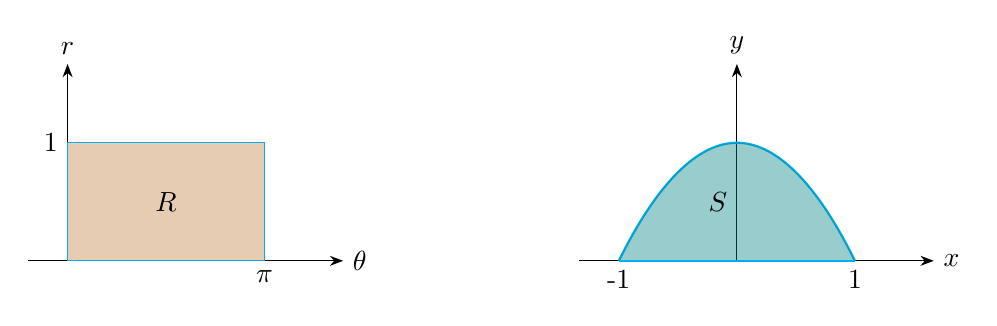
\begin{tikzpicture}[=>stealth]
\draw[-Stealth](-0.5,0)--(3.5,0)node[right]{$\theta$};
\draw[-Stealth](0,0)--(0,2.5)node[above]{$r$};
\path[fill=brown,opacity=0.4](0,0)--(2.5,0)--(2.5,1.5)--(0,1.5)--cycle;
\draw[cyan](0,0)rectangle(2.5,1.5);
\draw(2.5,0)node[below]{$\pi$}
(0,1.5)node[left]{$1$}
(1.25,0.75)node[]{$R$};
\draw[-Stealth](6.5,0)--(11,0)node[right]{$x$};
\draw[-Stealth](8.5,0)--(8.5,2.5)node[above]{$y$};
\draw[thick,cyan](8.5,1.5)parabola(10,0);
\draw[thick,cyan](8.5,1.5)parabola(7,0);
\path[fill=teal,opacity=0.4](8.5,1.5)parabola(10,0)--(8.5,0)--(8.5,1.5)parabola(7,0)--(8.5,0);
\draw[thick,cyan](7,0)--(10,0);
\draw(7,0)node[below]{-1}
(10,0)node[below]{1}
(8.5,0.75)node[left]{$S$};
\end{tikzpicture}
\end{figure}

The whole edge $r = 0$ of $R$ is sent to the single point $(0,0)$, so the
mapping is not one-to-one there; this is where its Jacobian, $r$, vanishes.

A mapping $f: \mathbb{R}^n \to \mathbb{R}^m$ is a \emph{linear transformation} if
\begin{enumerate}
\item $f(\mathbf x+\mathbf y) = f(\mathbf x) + f(\mathbf y)$ for all
$\mathbf x,\mathbf y \in \mathbb{R}^n$, and

\item $f(\alpha \mathbf x) = \alpha f(\mathbf x)$ for every scalar $\alpha$ and
every $\mathbf x \in \mathbb{R}^n$.
\end{enumerate}
Every linear transformation from $\mathbb{R}^n$ to $\mathbb{R}^m$ is
multiplication by an $m\times n$ matrix $A$, $f(\mathbf x) = A\mathbf x$, as in
Example~\ref{ex:linearmap}; the columns of $A$ are the images of the standard
basis vectors. The polar mapping is not linear, since
$f(2r,2\theta)\neq 2f(r,\theta)$ in general.
\end{solution}

\begin{exa}
\label{ex:mapdomains}
Let $f,g: \mathbb{R}^3 \to \mathbb{R}^2$ be given by
\[f(x,y,z) =\left(\sqrt{1 - x^2 - y^2 -z^2},\ xy^2z^3\right),\qquad g(x,y,z) =
\left(\frac{1}{x + y + z},\ \sqrt{x}\right).\]
Compute $-4f$ and $f+g$ and determine their domains.
\end{exa}

\begin{solution}
The domain of $f$ is the closed unit ball $\{(x,y,z) \mid x^2 + y^2 + z^2 \leq
1\}$, and
\[-4f =\left(-4\sqrt{1 - x^2 - y^2 -z^2},\ -4 xy^2z^3\right)\]
has the same domain. The sum is formed component by component,
\[f +g =\left(\sqrt{1 - x^2 - y^2 -z^2} + \frac{1}{x + y + z},\ xy^2z^3 +
\sqrt{x}\right),\]
and is defined where both $f$ and $g$ are:
\[\{ (x,y,z) \mid x^2 + y^2 + z^2 \leq 1,\ x+y+z\neq 0,\ x\geq 0\}.\]
\end{solution}

\begin{defn}
\label{defn:jacobianmap}
Let $f: \mathbb{R}^n \to \mathbb{R}^m$ have components with first partial
derivatives at $\mathbf x$. Its \emph{Jacobian matrix} at $\mathbf x$ is the
$m\times n$ matrix $J_f(\mathbf x) = \left(\frac{\partial f_i}{\partial
x_j}(\mathbf x)\right)$. When $m = n$, the \emph{Jacobian} of the mapping is the
determinant $\det J_f(\mathbf x)$.
\end{defn}

The Jacobian matrix is the matrix of the best linear approximation to $f$ near
$\mathbf x$:
$f(\mathbf x + \mathbf h)\approx f(\mathbf x) + J_f(\mathbf x)\,\mathbf h$, each
row being the tangent-plane approximation of one component.

\begin{defn}
\label{defn:locallyinvertible}
Let $f: \mathbb{R}^n \to \mathbb{R}^n$ have continuous first partial derivatives
on an open set $\Omega$ (written $f\in C^1(\Omega)$). Then $f$ is \emph{locally
$C^1$-invertible} on $\Omega$ if $f$ is one-to-one on $\Omega$ and there is a
function $g\in C^1(f(\Omega))$ such that
\[(g\circ f)(\mathbf x) = \mathbf x\ \text{for every}\ \mathbf x\in
\Omega,\qquad (f\circ g)(\mathbf y) = \mathbf y\ \text{for every}\ \mathbf y \in
f(\Omega) ;\]
that is, $g = f^{-1}$ on $f(\Omega)$.
\end{defn}

For a linear transformation $f(\mathbf x) = A\mathbf x$, the inverse is
$f^{-1}(\mathbf y) = A^{-1}\mathbf y$, which exists exactly when
$\det A\neq 0$. The inverse function theorem of the next subsection says that
the same is true locally of any $C^1$ mapping, with $A$ replaced by the Jacobian
matrix.

\begin{exa}
\label{ex:jacobianmatrix3}
Find the Jacobian matrix of $f(x,y,z) = (x^2 + yz,\ xe^{y},\ \sin(xz))$ at
$(1,0,\pi)$, and use it to approximate $f(1.01, 0.02, \pi)$.
\end{exa}

\begin{solution}
\[J_f = \begin{pmatrix} 2x & z & y\\ e^y & xe^y & 0\\ z\cos(xz) & 0 &
x\cos(xz)\end{pmatrix},\qquad J_f(1,0,\pi) = \begin{pmatrix} 2 & \pi & 0\\ 1 & 1
& 0\\ -\pi & 0 & -1\end{pmatrix} .\]
With $f(1,0,\pi) = (1, 1, 0)$ and $\mathbf h = (0.01, 0.02, 0)$,
\[f(1.01,0.02,\pi)\approx (1,1,0) + (0.02 + 0.0628,\ 0.01 + 0.02,\ -0.0314) =
(1.0828,\ 1.03,\ -0.0314).\]
The exact values are $(1.0829, 1.0304, -0.0314)$ to four decimal places.
\end{solution}

{\color[wave]{485}\subsection{Inverse Function Theorem}}

\begin{thm}[Inverse function theorem]
\label{thm:inverse}
Let $f: \mathbb{R}^n \to \mathbb{R}^n$ be in $C^1(\Omega)$ on an open set
$\Omega$, and let $\mathbf x_0\in\Omega$. If the Jacobian
$\det J_f(\mathbf x_0)$ is not zero, then there is an open set
$\Omega_1 \subseteq \Omega$ containing $\mathbf x_0$ on which $f$ is locally
$C^1$-invertible. Moreover, if $g = f^{-1}$ on $f(\Omega_1)$, then
\[J_g(f(\mathbf x_0)) = \big(J_f(\mathbf x_0)\big)^{-1} .\]
\end{thm}

The existence of the inverse follows from the implicit function theorem applied
to the $n$ equations $f_i(\mathbf x) - y_i = 0$, regarded as equations for
$\mathbf x$ in terms of $\mathbf y$: the Jacobian with respect to $\mathbf x$ is
$\det J_f(\mathbf x_0)\neq 0$. The formula for the derivative then follows from
the general chain rule: differentiating $g(f(\mathbf x)) = \mathbf x$ gives
$J_g(f(\mathbf x))\,J_f(\mathbf x) = I$, the identity matrix. Note that the
Jacobian of the inverse is evaluated at the image point $f(\mathbf x_0)$.

\begin{exa}
\label{ex:polarinverse}
Show that the polar transformation $f(r,\theta) = (r\cos\theta, r\sin\theta)$ is
locally invertible at every point with $r\neq 0$, and find the Jacobian matrix of
the inverse.
\end{exa}

\begin{solution}
\[J_f(r,\theta) = \begin{pmatrix}
\cos \theta & - r\sin \theta\\
\sin \theta & r\cos \theta
\end{pmatrix},\qquad \det J_f = r\cos^2\theta + r\sin^2\theta = r .\]
So $f$ is locally invertible wherever $r\neq 0$, and by
Theorem~\ref{thm:inverse} the inverse has Jacobian matrix
\[\big(J_f(r,\theta)\big)^{-1} = \frac{1}{r}\begin{pmatrix}
r\cos \theta & r \sin \theta \\
-\sin \theta & \cos \theta
\end{pmatrix} =
\begin{pmatrix}
\cos \theta & \sin \theta\\
-\frac{\sin \theta}{r} & \frac{\cos \theta}{r}
\end{pmatrix} ,\]
the rows giving $\left(\frac{\partial r}{\partial x}, \frac{\partial r}{\partial
y}\right)$ and $\left(\frac{\partial \theta}{\partial x}, \frac{\partial
\theta}{\partial y}\right)$. As a check, $r = \sqrt{x^2+y^2}$ gives
$\frac{\partial r}{\partial x} = \frac{x}{r} = \cos\theta$. The theorem gives
only local invertibility: $f$ is not one-to-one on the whole half-plane $r>0$,
since $\theta$ and $\theta + 2\pi$ have the same image.
\end{solution}

\begin{exa}
\label{ex:inverselocal}
Show that $f(x,y) = (e^x\cos y,\ e^x\sin y)$ has non-zero Jacobian everywhere but
is not one-to-one on $\mathbb{R}^2$.
\end{exa}

\begin{solution}
\[\det J_f = \begin{vmatrix} e^x\cos y & -e^x\sin y\\ e^x\sin y & e^x\cos
y\end{vmatrix} = e^{2x}>0 .\]
So $f$ is locally invertible near every point. But $f(x, y + 2\pi) = f(x,y)$, so
$f$ is not one-to-one on the plane. (In complex notation $f$ is
$z\mapsto e^z$.) A non-vanishing Jacobian guarantees an inverse near each point,
not a global one; in one variable the two coincide, but in two or more they do
not.
\end{solution}

\begin{exa}
\label{ex:inversederiv}
Let $u = x + y^3$, $v = x^3 - y$. Find $\frac{\partial x}{\partial u}$ and
$\frac{\partial y}{\partial v}$ at the point where $(x,y) = (1,1)$.
\end{exa}

\begin{solution}
\[J = \begin{pmatrix} u_x & u_y\\ v_x & v_y\end{pmatrix} = \begin{pmatrix} 1 &
3y^2\\ 3x^2 & -1\end{pmatrix} = \begin{pmatrix} 1 & 3\\ 3 &
-1\end{pmatrix}\ \text{at}\ (1,1),\]
with determinant $-10\neq 0$. By Theorem~\ref{thm:inverse},
\[\begin{pmatrix} x_u & x_v\\ y_u & y_v\end{pmatrix} = J^{-1} = -\frac{1}{10}
\begin{pmatrix} -1 & -3\\ -3 & 1\end{pmatrix} = \begin{pmatrix} \frac{1}{10} &
\frac{3}{10}\\ \frac{3}{10} & -\frac{1}{10}\end{pmatrix},\]
so $\frac{\partial x}{\partial u} = \frac{1}{10}$ and
$\frac{\partial y}{\partial v} = -\frac{1}{10}$. Note that
$\frac{\partial x}{\partial u}\neq\frac{1}{\partial u/\partial x} = 1$: the
reciprocal rule holds for whole Jacobian matrices, not for individual partial
derivatives.
\end{solution}

{\color[wave]{485}\subsection{Functional Dependence}}

\begin{defn}
\label{defn:dependent}
Two functions $u(x,y)$ and $v(x,y)$ are \emph{functionally dependent} on a region
if there is a function $\Phi$, not identically zero on any open set, with
$\Phi(u(x,y),v(x,y)) = 0$ throughout the region; for example, $u = g(v)$ or
$v = h(u)$.
\end{defn}

Dependent functions carry the same information: knowing one determines the
other. The Jacobian detects this.

\begin{thm}
\label{thm:dependence}
If $u$ and $v$ have continuous partial derivatives and are functionally dependent
through a differentiable $\Phi$ whose gradient is never zero, then
\[\frac{\partial (u,v)}{\partial (x,y)} = 0\]
throughout the region. Conversely, if this Jacobian vanishes identically on an
open region in which $\nabla u\neq\mathbf 0$, then $u$ and $v$ are functionally
dependent there.
\end{thm}

\begin{proof}[Proof of the first part]
Differentiating $\Phi(u,v) = 0$ with respect to $x$ and $y$,
\[\Phi_u\,u_x + \Phi_v\,v_x = 0,\qquad \Phi_u\,u_y + \Phi_v\,v_y = 0,\]
that is,
\[\begin{pmatrix}
u_x & v_x\\
u_y & v_y
\end{pmatrix}
\begin{pmatrix}
\Phi_u\\
\Phi_v
\end{pmatrix}
= \begin{pmatrix} 0\\ 0\end{pmatrix}.\]
The vector $(\Phi_u,\Phi_v)$ is never zero, so this homogeneous system has a
non-trivial solution, and its determinant must vanish. That determinant is the
transpose of the Jacobian matrix, and $\det A^{\mathsf T} = \det A$, so
$\frac{\partial(u,v)}{\partial(x,y)} = 0$.
\end{proof}

For the converse, the condition $\nabla u\neq\mathbf 0$ allows $u$ to be used as
a new coordinate near each point. The vanishing Jacobian then says that $v$ does
not change along the level curves of $u$, so $v$ is a function of $u$ alone. The
same results hold for $n$ functions of $n$ variables, with the $n\times n$
Jacobian.

\begin{exa}
\label{ex:dependent3}
Determine whether the following are functionally dependent:
\[u = y + z,\qquad v = x + 2z^2,\qquad w = x - 4yz - 2y^2 .\]
\end{exa}

\begin{solution}
\[\frac{\partial (u,v,w)}{\partial (x,y,z)} = \begin{vmatrix}
0 & 1 & 1\\
1 & 0 & 4z\\
1 & -4z - 4y & -4y
\end{vmatrix} = 0 - 1\,(-4y - 4z) + 1\,(-4z - 4y) = 0 .\]
So $u$, $v$, $w$ are functionally dependent. To find the relation, note that
$v - w = 2z^2 + 4yz + 2y^2 = 2(y + z)^2 = 2u^2$, so $w = v - 2u^2$.
\end{solution}

\begin{exa}
\label{ex:dependentlog}
Determine whether $f(x,y) = e^x \sin y$ and $g(x,y) = x + \ln \sin y$ are
functionally dependent on the region $0<y<\pi$.
\end{exa}

\begin{solution}
\[\frac{\partial (f,g)}{\partial (x,y)} = \begin{vmatrix}
e^x\sin y & e^x\cos y\\
1 & \cot y
\end{vmatrix} = e^x\sin y\cot y - e^x\cos y = 0 ,\]
so $f$ and $g$ are functionally dependent; indeed $\ln f = x + \ln\sin y = g$.
\end{solution}

\begin{exa}
\label{ex:independent}
Show that $u = x + y$ and $v = x - y$ are independent, and find all $(x,y)$ at
which $u = x^2 + y^2$ and $v = xy$ fail the Jacobian test.
\end{exa}

\begin{solution}
For the first pair, $\frac{\partial(u,v)}{\partial(x,y)} = \begin{vmatrix} 1 & 1\\
1 & -1\end{vmatrix} = -2\neq 0$, so they are independent everywhere. For the
second,
\[\frac{\partial(u,v)}{\partial(x,y)} = \begin{vmatrix} 2x & 2y\\ y &
x\end{vmatrix} = 2(x^2 - y^2),\]
which vanishes only on the lines $y = \pm x$. Since it is not identically zero,
$u$ and $v$ are independent, but on those lines they are locally related: for
$y = x$, $u = 2x^2 = 2v$. These are exactly the lines where the mapping
$(x,y)\mapsto(u,v)$ fails to be locally invertible, folding the plane over.
\end{solution}

\begin{exa}
\label{ex:dependentarctan}
Show that $u = \frac{x - y}{1 + xy}$ and $v = \tan^{-1}x - \tan^{-1}y$ are
functionally dependent, and find the relation.
\end{exa}

\begin{solution}
\[u_x = \frac{(1 + xy) - (x - y)y}{(1 + xy)^2} = \frac{1 + y^2}{(1 + xy)^2},
\qquad u_y = \frac{-(1 + xy) - (x - y)x}{(1 + xy)^2} = -\frac{1 + x^2}{(1 +
xy)^2},\]
and $v_x = \frac{1}{1 + x^2}$, $v_y = -\frac{1}{1 + y^2}$, so
\[\frac{\partial(u,v)}{\partial(x,y)} = -\frac{1 + y^2}{(1 + xy)^2(1 + y^2)} +
\frac{1 + x^2}{(1 + xy)^2(1 + x^2)} = 0 .\]
By the subtraction formula for the tangent, $\tan v = \frac{x - y}{1 + xy} = u$.
\end{solution}


\subsection{Practice Problems}

Each problem is worked in full.

\begin{problem}
Find the domain and range of each function, and sketch the domain where
possible.
\[(a)\ z = \frac{\sqrt{x^2+y^2-9}}{x-y}\qquad 
(b)\ z = \frac{3}{\sqrt{x^2-y}}\qquad 
(c)\ z = \tan^{-1}\left(\frac{y}{x}\right)\]
\end{problem}
\begin{solution}
\subhead{(a)}
The square root needs $x^2+y^2\geq 9$ and the denominator must not vanish, so
\[\text{domain} = \{(x,y): x^2+y^2\geq 9,\ y\neq x\},\]
the closed exterior of the circle of radius $3$ with the line $y=x$ removed. On
that set the numerator takes every value in $[0,\infty)$ and the denominator
every non-zero value of either sign, so the range is all of $\mathbb{R}$.

\subhead{(b)}
The square root must be defined and non-zero, so $x^2-y>0$, that is
\[\text{domain} = \{(x,y): y < x^2\},\]
the open region below the parabola $y = x^2$. Since $x^2-y$ takes every value in
$(0,\infty)$, the range is $(0,\infty)$.

\subhead{(c)}
Only $x=0$ is excluded, so the domain is the whole plane less the $y-$axis. The
inverse tangent takes values in $\left(-\dfrac{\pi}{2}, \dfrac{\pi}{2}\right)$, and
every such value is attained, so that is the range.
\end{solution}

\begin{problem}
Sketch the family of level curves of each surface, label them, and use them to
sketch the surface.
\begin{gather*}
(a)\ z = \sqrt{13-x^2-y^2}\qquad (b)\ z = x^2+y^2-1\qquad (c)\ z = 7-x^2-y^2\\
(d)\ z = 2x^2-1\qquad (e)\ z = \arctan(x^2+y^2)
\end{gather*}
\end{problem}
\begin{solution}
A level curve is the set where $z$ takes a fixed value $k$; the surface is
recovered by stacking them at their heights.

\subhead{(a)}
$k = \sqrt{13-x^2-y^2}$ gives $x^2+y^2 = 13-k^2$, circles of radius
$\sqrt{13-k^2}$ for $0\leq k\leq\sqrt{13}$. They shrink to a point at the top:
the surface is the upper half of the sphere of radius $\sqrt{13}$.

\subhead{(b)}
$x^2+y^2 = k+1$, circles of radius $\sqrt{k+1}$ existing only for $k\geq -1$.
Equally spaced values of $k$ give circles that crowd together as $k$ grows: a
circular paraboloid opening upward with vertex $(0,0,-1)$.

\subhead{(c)}
$x^2+y^2 = 7-k$, circles for $k\leq 7$: a paraboloid opening \emph{downward}
with vertex $(0,0,7)$.

\subhead{(d)}
$2x^2 = k+1$ gives $x = \pm\sqrt{\dfrac{k+1}{2}}$, pairs of vertical lines. $y$
is absent, so the surface is a parabolic cylinder: the parabola $z = 2x^2-1$
translated along the $y-$axis.

\subhead{(e)}
$x^2+y^2 = \tan k$, circles for $0\leq k<\dfrac{\pi}{2}$. The radii grow without
bound as $k$ approaches $\dfrac{\pi}{2}$, so the surface rises steeply near the
axis and then flattens towards the horizontal plane $z = \dfrac{\pi}{2}$, which
it never reaches.
\end{solution}

\begin{problem}
Show that $\displaystyle{\lim_{(x,y)\rightarrow(0,0)}\frac{4x^2y^3}{x^3+y^9}}$
does not exist.
\end{problem}
\begin{solution}
Along $y=0$ the function is identically $0$, so that path gives $0$.

Now approach along the curve $x = y^3$, which passes through the origin. There
\[\frac{4(y^3)^2y^3}{(y^3)^3+y^9}
= \frac{4y^9}{y^9+y^9} = \frac{4y^9}{2y^9} = 2 ,\]
constant, so that path gives $2$.

Two paths give different values, so no limit exists.

Note that every straight line $y = mx$ gives $0$ here, so testing lines alone
would have suggested the limit was $0$. The cubic path is what exposes it, and
choosing it is guided by making the two terms of the denominator the same order.
\end{solution}

\begin{problem}
The height in metres at $(x,y)$ on a mountain is $h(x,y) = 1400-x^2-y^2$. A
mountaineer stands above $(10,20)$. Find the direction in which the height
(a) increases most rapidly, (b) decreases most rapidly, (c) does not change.
\end{problem}
\begin{solution}
\[\nabla h = \langle -2x, -2y\rangle
\ \longrightarrow\ \nabla h(10,20) = \langle -20, -40\rangle .\]

\subhead{(a)} Steepest increase is along the gradient,
$\langle -20,-40\rangle$, or as a unit vector
$-\dfrac{1}{\sqrt5}\langle 1,2\rangle$ --- towards the summit, as expected since
the peak is at the origin.

\subhead{(b)} Steepest decrease is the opposite direction,
$\dfrac{1}{\sqrt5}\langle 1,2\rangle$.

\subhead{(c)} No change occurs perpendicular to the gradient, along
$\pm\dfrac{1}{\sqrt5}\langle 2,-1\rangle$. On a contour map these are the
directions along the contour through the point, while (a) and (b) cross the
contours at right angles.
\end{solution}

\begin{problem}
The electrical potential is $V(x,y,z) = 5x^2-3xy+xyz$.
\begin{enumerate}
\item[(a)] Find the rate of change at $P(3,4,5)$ in the direction of
$\langle 1,1,-1\rangle$.
\item[(b)] In which direction does $V$ change most rapidly?
\item[(c)] What is the maximum rate of change?
\end{enumerate}
\end{problem}
\begin{solution}
\[V_x = 10x-3y+yz,\qquad V_y = -3x+xz,\qquad V_z = xy ,\]
so at $(3,4,5)$,
\[\nabla V = \langle 30-12+20,\ -9+15,\ 12\rangle = \langle 38, 6, 12\rangle .\]

\subhead{(a)}
The unit vector in the given direction is
$\dfrac{1}{\sqrt3}\langle 1,1,-1\rangle$, so
\[D_{\mathbf{u}}V = \nabla V\cdot\mathbf{u}
= \frac{38+6-12}{\sqrt3} = \frac{32}{\sqrt3} = \frac{32\sqrt3}{3}\approx 18.5 .\]

\subhead{(b)}
Most rapidly along $\nabla V = \langle 38,6,12\rangle$ itself.

\subhead{(c)}
The maximum rate is
$\left|\nabla V\right| = \sqrt{1444+36+144} = \sqrt{1624} = 2\sqrt{406}
\approx 40.3$.
\end{solution}

\begin{problem}
Find and classify the stationary points of $f(x,y) = 2x^3-x^2y+y^2$.
\end{problem}
\begin{solution}
\[f_x = 6x^2-2xy = 2x(3x-y) = 0,\qquad f_y = -x^2+2y = 0 .\]
The second gives $y = \dfrac{x^2}{2}$. Substituting into the first,
$2x\left(3x-\dfrac{x^2}{2}\right) = 0$, so $x = 0$ or $x = 6$. The stationary
points are $(0,0)$ and $(6,18)$.

The second partials are $f_{xx} = 12x-2y$, $f_{yy} = 2$, $f_{xy} = -2x$, so
\[D = 2(12x-2y) - 4x^2 .\]
At $(6,18)$: $D = 2(72-36)-144 = -72 < 0$, a \emph{saddle point}.

At $(0,0)$: $D = 0$, so the test is inconclusive. Examine the function directly.
Along $y=0$, $f = 2x^3$, which changes sign at the origin, taking both positive
and negative values arbitrarily close to it. Hence $(0,0)$ is neither a maximum
nor a minimum: it too is a \emph{saddle}.
\end{solution}

\begin{problem}
An open rectangular box is to be made from $12\ \text{m}^2$ of cardboard. Find
its maximum volume.
\end{problem}
\begin{solution}
Let the base be $a$ by $b$ and the height $c$. With no lid the surface area is
\[ab + 2ac + 2bc = 12 ,\]
and the volume $V = abc$ is to be maximised. By Lagrange multipliers,
$\nabla V = \lambda\nabla g$ gives
\[bc = \lambda(b+2c),\qquad ac = \lambda(a+2c),\qquad ab = \lambda(2a+2b).\]
Multiplying the first by $a$ and the second by $b$ and subtracting,
$\lambda(ab+2ac-ab-2bc) = 0$, so $a = b$ (taking $\lambda\neq 0$).
Substituting $a=b$ into the constraint and the third equation gives
\[a = b = 2,\qquad c = 1 ,\]
so the maximum volume is $V = 2\cdot 2\cdot 1 = 4\ \text{m}^3$. Note the base is
square and the height is half the base, which is the general shape for a lidless
box of fixed area.
\end{solution}

\begin{problem}
Find and classify the stationary points of
$f(x,y) = \exp\left(-\dfrac13x^3 + x - y^2\right)$.
\end{problem}
\begin{solution}
Write $f = e^{g}$ with $g = -\dfrac13x^3+x-y^2$. Since the exponential is never
zero and always positive, $\nabla f = f\nabla g$ vanishes exactly where
$\nabla g$ does, and $f$ has a maximum or minimum precisely where $g$ does.
\[g_x = -x^2+1 = 0 \implies x = \pm 1,\qquad g_y = -2y = 0 \implies y = 0 .\]
For $g$: $g_{xx} = -2x$, $g_{yy} = -2$, $g_{xy} = 0$, so $D = 4x$.

At $(1,0)$: $D = 4>0$ and $g_{xx} = -2<0$, a \emph{local maximum}, with
$f = e^{2/3}$.

At $(-1,0)$: $D = -4<0$, a \emph{saddle point}, with $f = e^{-2/3}$.

Working through $g$ rather than $f$ avoids differentiating the exponential
twice, and is legitimate because $t\mapsto e^t$ is strictly increasing.
\end{solution}

\begin{problem}
Let $g(x,y) = 2(x^2+y^2)e^{-(x^2+y^2)}$.
\begin{enumerate}
\item[(a)] Find all stationary points, without using the second derivative test.
\item[(b)] For which $(x,y)$ is $g(x,y)<0$?
\item[(c)] What happens as $x$ and $y$ both tend to infinity?
\item[(d)] Use (b) and (c) to classify the stationary points.
\item[(e)] Describe the surface $z = g(x,y)$.
\end{enumerate}
\end{problem}
\begin{solution}
The function depends only on $r^2 = x^2+y^2$, so write
$G(r) = 2r^2e^{-r^2}$ with $r\geq 0$.

\subhead{(a)}
\[G'(r) = 4re^{-r^2} - 4r^3e^{-r^2} = 4re^{-r^2}(1-r^2) = 0\]
gives $r=0$ or $r=1$. So the stationary points are the origin and every point of
the circle $x^2+y^2 = 1$ --- a whole curve of them, which is why the second
derivative test is not the tool here.

\subhead{(b)}
Never. Both $2r^2$ and $e^{-r^2}$ are non-negative, so $g\geq 0$ everywhere,
with equality only at the origin.

\subhead{(c)}
$G(r) = \dfrac{2r^2}{e^{r^2}}\rightarrow 0$ as $r\rightarrow\infty$, since the
exponential outgrows any power.

\subhead{(d)}
By (b), $g\geq 0$ with equality only at the origin, so the origin is the
absolute \emph{minimum}. On the circle $r=1$, $g = 2e^{-1}\approx 0.736$; since
$g$ increases from $0$ to that value as $r$ goes from $0$ to $1$ and decreases
back towards $0$ afterwards, every point of the circle is an absolute
\emph{maximum}.

\subhead{(e)}
A surface of revolution: a dip to zero at the origin, rising to a circular
crest of height $2e^{-1}$ above the unit circle, then falling away
asymptotically to the plane $z=0$ --- the shape of a volcano rim.
\end{solution}

\begin{problem}
Find the dimensions of the largest box, with edges parallel to the axes, that
fits inside the ellipsoid
$\dfrac{x^2}{a^2}+\dfrac{y^2}{b^2}+\dfrac{z^2}{c^2} = 1$.
\end{problem}
\begin{solution}
By symmetry the box is centred at the origin, so if one corner is $(x,y,z)$ in
the first octant the box has edges $2x$, $2y$, $2z$ and volume $V = 8xyz$.
Maximise subject to the corner lying on the ellipsoid. Lagrange gives
\[8yz = \frac{2\lambda x}{a^2},\qquad 8xz = \frac{2\lambda y}{b^2},
\qquad 8xy = \frac{2\lambda z}{c^2}.\]
Multiplying the first by $x$, the second by $y$ and the third by $z$ shows all
three of $\dfrac{x^2}{a^2}$, $\dfrac{y^2}{b^2}$, $\dfrac{z^2}{c^2}$ equal, so
each is $\dfrac13$ by the constraint. Hence
\[x = \frac{a}{\sqrt3},\qquad y = \frac{b}{\sqrt3},\qquad z = \frac{c}{\sqrt3},\]
the box has dimensions $\dfrac{2a}{\sqrt3}\times\dfrac{2b}{\sqrt3}\times
\dfrac{2c}{\sqrt3}$, and
\[V = \frac{8abc}{3\sqrt3} = \frac{8\sqrt3}{9}abc\approx 1.54\,abc .\]
For a sphere ($a=b=c$) this is the cube, as it must be.
\end{solution}

\begin{problem}
Use Lagrange multipliers to find the maximum and minimum of $f(x,y,z) = xyz$
subject to $x^2+2y^2+3z^2 = 6$.
\end{problem}
\begin{solution}
The conditions $\nabla f = \lambda\nabla g$ read
\[yz = 2\lambda x,\qquad xz = 4\lambda y,\qquad xy = 6\lambda z .\]
Multiplying each by the corresponding variable gives
\[xyz = 2\lambda x^2 = 4\lambda y^2 = 6\lambda z^2 .\]
If $\lambda = 0$ then $xyz = 0$, giving the value $0$. Otherwise
\[x^2 = 2y^2 = 3z^2 ,\]
and substituting into the constraint, $x^2+x^2+x^2 = 6$, so $x^2 = 2$ and
\[x = \pm\sqrt2,\qquad y = \pm 1,\qquad z = \pm\sqrt{\tfrac23}.\]
At such a point
\[\left|xyz\right| = \sqrt2\cdot 1\cdot\sqrt{\tfrac23} = \frac{2}{\sqrt3}
= \frac{2\sqrt3}{3}\approx 1.155 .\]
Choosing the signs so the product is positive gives the maximum
$\dfrac{2\sqrt3}{3}$, and so the product is negative gives the minimum
$-\dfrac{2\sqrt3}{3}$.
\end{solution}

\begin{problem}
Let $f(x,y) = xy^2+\ln(1+xy)$.
\begin{enumerate}
\item[(a)] Find the Taylor polynomial to second degree about $(1,1)$.
\item[(b)] Write the tangent plane to $z = f(x,y)$ at $x=1$, $y=1$.
\item[(c)] Find the stationary points, and classify only $(0,0)$.
\end{enumerate}
\end{problem}
\begin{solution}
\subhead{The derivatives at $(1,1)$}
\[f_x = y^2 + \frac{y}{1+xy},\qquad f_y = 2xy + \frac{x}{1+xy},\]
so $f(1,1) = 1+\ln 2$, $f_x(1,1) = 1+\dfrac12 = \dfrac32$ and
$f_y(1,1) = 2+\dfrac12 = \dfrac52$. Differentiating again,
\[f_{xx} = -\frac{y^2}{(1+xy)^2} \rightarrow -\frac14,\qquad
f_{yy} = 2x - \frac{x^2}{(1+xy)^2} \rightarrow \frac74,\]
\[f_{xy} = 2y + \frac{1}{(1+xy)^2} \rightarrow \frac94 .\]

\subhead{(a)}
With $h = x-1$ and $k = y-1$,
\[f \approx 1+\ln 2 + \frac32h + \frac52k
+ \frac12\left[-\frac14h^2 + 2\cdot\frac94hk + \frac74k^2\right]\]
\[= 1+\ln 2 + \frac32h + \frac52k - \frac{h^2}{8} + \frac{9hk}{4}
+ \frac{7k^2}{8}.\]

\subhead{(b)}
The tangent plane is the linear part of that expansion:
\[z = 1+\ln 2 + \frac32(x-1) + \frac52(y-1).\]

\subhead{(c)}
Stationary points satisfy
\[y^2 + \frac{y}{1+xy} = 0,\qquad 2xy + \frac{x}{1+xy} = 0 .\]
Both hold when $x=y=0$, so $(0,0)$ is stationary. There
\[f_{xx}(0,0) = 0,\qquad f_{yy}(0,0) = 0,\qquad f_{xy}(0,0) = 1 ,\]
so $D = 0\cdot 0 - 1 = -1 < 0$ and $(0,0)$ is a \emph{saddle point}.
\end{solution}


\begin{problem}
Let $f(x,y) = x^3+y^2-3xy+y$.
\begin{enumerate}
\item[(a)] Locate and classify the stationary points.
\item[(b)] Find the global maximum and minimum over
$R = \{(x,y): 0\leq x\leq 2,\ 0\leq y\leq 2\}$.
\end{enumerate}
\end{problem}
\begin{solution}
\subhead{(a)}
\[f_x = 3x^2-3y = 0 \implies y = x^2,\qquad
f_y = 2y-3x+1 = 0 .\]
Substituting, $2x^2-3x+1 = 0$, so $(2x-1)(x-1) = 0$ and
$x = \dfrac12$ or $x = 1$. The stationary points are
$\left(\dfrac12,\dfrac14\right)$ and $(1,1)$.

With $f_{xx} = 6x$, $f_{yy} = 2$, $f_{xy} = -3$, the discriminant is
$D = 12x-9$.

At $\left(\dfrac12,\dfrac14\right)$: $D = -3<0$, a \emph{saddle}, value
$\dfrac{1}{16}$.

At $(1,1)$: $D = 3>0$ and $f_{xx} = 6>0$, a \emph{local minimum}, value $0$.

\subhead{(b)}
Both stationary points lie in $R$, contributing $\dfrac{1}{16}$ and $0$. Now the
four edges.

On $y=0$: $f = x^3$, running from $0$ to $8$.

On $y=2$: $f = x^3-6x+6$, with $f' = 3x^2-6 = 0$ at $x = \sqrt2$, giving
$6-4\sqrt2\approx 0.34$; the endpoints give $6$ and $2$.

On $x=0$: $f = y^2+y$, from $0$ to $6$.

On $x=2$: $f = 8+y^2-6y+y = y^2-5y+8$, minimised at $y = \dfrac52$ which is
outside $[0,2]$, so the endpoints give $8$ and $2$.

Comparing every candidate, the global minimum is $0$, attained at $(1,1)$ and at
the origin, and the global maximum is $8$, at $(2,0)$.
\end{solution}

\begin{problem}
Find the absolute maximum and minimum of $z = x^2+2y^2-x$ on the disc
$x^2+y^2\leq 1$.
\end{problem}
\begin{solution}
\subhead{Interior}
$z_x = 2x-1 = 0$ and $z_y = 4y = 0$ give $\left(\dfrac12, 0\right)$, inside the
disc, with $z = \dfrac14-\dfrac12 = -\dfrac14$.

\subhead{Boundary}
On $x^2+y^2 = 1$ substitute $y^2 = 1-x^2$:
\[z = x^2+2(1-x^2)-x = 2-x^2-x ,\qquad -1\leq x\leq 1 .\]
Then $\dfrac{dz}{dx} = -2x-1 = 0$ at $x = -\dfrac12$, giving
$z = 2-\dfrac14+\dfrac12 = \dfrac94$. The endpoints give $z = 0$ at $x=1$ and
$z = 2$ at $x=-1$.

\subhead{Conclusion}
The absolute minimum is $-\dfrac14$ at $\left(\dfrac12,0\right)$, and the absolute
maximum is $\dfrac94$ at $\left(-\dfrac12, \pm\dfrac{\sqrt3}{2}\right)$.
\end{solution}

\begin{problem}
Use Lagrange multipliers to find the maximum and minimum of $f(x,y,z) = x+2y$
subject to $x+y+z = 1$ and $y^2+z^2 = 4$.
\end{problem}
\begin{solution}
With two constraints, $\nabla f = \lambda\nabla g + \mu\nabla h$ where
$g = x+y+z$ and $h = y^2+z^2$:
\[1 = \lambda,\qquad 2 = \lambda + 2\mu y,\qquad 0 = \lambda + 2\mu z .\]
From the first, $\lambda = 1$. The second gives $2\mu y = 1$ and the third
$2\mu z = -1$, so $\mu\neq 0$ and
\[y = \frac{1}{2\mu},\qquad z = -\frac{1}{2\mu},\qquad\text{hence } z = -y .\]
Substituting into $y^2+z^2 = 4$ gives $2y^2 = 4$, so
$y = \pm\sqrt2$ and $z = \mp\sqrt2$. The first constraint then gives
$x = 1-y-z = 1$.

The two candidate points are $(1, \sqrt2, -\sqrt2)$ and
$(1, -\sqrt2, \sqrt2)$, where
\[f = 1+2\sqrt2 \approx 3.83 \qquad\text{and}\qquad f = 1-2\sqrt2\approx -1.83 .\]
These are the maximum and minimum respectively.
\end{solution}

\begin{problem}
Find the points on the sphere $x^2+y^2+z^2 = 4$ closest to and farthest from
$(3,1,-1)$.
\end{problem}
\begin{solution}
The extreme points lie on the line through the centre and the given point, which
saves the Lagrange calculation. The point is at distance
\[\left|\langle 3,1,-1\rangle\right| = \sqrt{9+1+1} = \sqrt{11}\approx 3.317\]
from the origin, which exceeds the radius $2$, so it lies outside the sphere.

The unit vector towards it is $\dfrac{1}{\sqrt{11}}\langle 3,1,-1\rangle$, so
the nearest point is
\[\frac{2}{\sqrt{11}}\langle 3,1,-1\rangle
= \left(\frac{6}{\sqrt{11}}, \frac{2}{\sqrt{11}}, -\frac{2}{\sqrt{11}}\right),\]
at distance $\sqrt{11}-2\approx 1.32$, and the farthest is the antipode
\[-\frac{2}{\sqrt{11}}\langle 3,1,-1\rangle ,\]
at distance $\sqrt{11}+2\approx 5.32$.
\end{solution}

\begin{problem}
Let $f(x,y) = x^3+y^3+3x^2-3y^2-8$.
\begin{enumerate}
\item[(a)] Find the Taylor expansion to second degree about $(0,0)$. What do you
observe?
\item[(b)] Write down, without further calculation, the expansion to third
degree about $(0,0)$.
\item[(c)] Find the expansion to second degree about $(1,2)$.
\end{enumerate}
\end{problem}
\begin{solution}
\subhead{(a)}
$f(0,0) = -8$; $f_x = 3x^2+6x$ and $f_y = 3y^2-6y$ both vanish at the origin;
$f_{xx} = 6x+6\rightarrow 6$, $f_{yy} = 6y-6\rightarrow -6$, $f_{xy} = 0$.
Hence
\[f \approx -8 + \frac12(6x^2 - 6y^2) = -8 + 3x^2 - 3y^2 .\]
The observation is that this is simply the part of $f$ of degree at most two,
read off from the original expression. A polynomial is its own Taylor
expansion about any point, so no work was necessary.

\subhead{(b)}
By the same observation, the third-degree expansion is the whole polynomial:
\[f = -8 + 3x^2 - 3y^2 + x^3 + y^3 ,\]
exact rather than approximate.

\subhead{(c)}
Here the expansion must be recomputed, since the powers of $x$ and $y$ are not
powers of $x-1$ and $y-2$. At $(1,2)$,
\[f = 1+8+3-12-8 = -8,\qquad f_x = 3+6 = 9,\qquad f_y = 12-12 = 0,\]
\[f_{xx} = 12,\qquad f_{yy} = 6,\qquad f_{xy} = 0 .\]
With $h = x-1$ and $k = y-2$,
\[f \approx -8 + 9h + \frac12(12h^2 + 6k^2) = -8 + 9h + 6h^2 + 3k^2 .\]
\end{solution}

\begin{problem}
Let $g(x,y) = \dfrac{1}{1+x^2+y^2}$.
\begin{enumerate}
\item[(a)] Find the second partial derivatives.
\item[(b)] Write the Taylor expansion to second degree about $(0,0)$.
\item[(c)] Use it to classify the stationary point $(0,0)$.
\item[(d)] Sketch the surface.
\end{enumerate}
\end{problem}
\begin{solution}
Write $s = 1+x^2+y^2$, so $g = s^{-1}$.

\subhead{(a)}
$g_x = -\dfrac{2x}{s^2}$ and $g_y = -\dfrac{2y}{s^2}$, so
\[g_{xx} = \frac{6x^2-2y^2-2}{s^3},\qquad
g_{yy} = \frac{6y^2-2x^2-2}{s^3},\qquad
g_{xy} = \frac{8xy}{s^3}.\]

\subhead{(b)}
At the origin $s=1$, so $g = 1$, both first derivatives vanish, and
$g_{xx} = g_{yy} = -2$ with $g_{xy} = 0$. Hence
\[g \approx 1 + \frac12(-2x^2 - 2y^2) = 1 - x^2 - y^2 .\]
The same result follows faster from the geometric series:
$\dfrac{1}{1+t} = 1-t+t^2-\cdots$ with $t = x^2+y^2$.

\subhead{(c)}
The quadratic part $-x^2-y^2$ is negative for every $(x,y)\neq(0,0)$, so $g$
decreases in every direction away from the origin: a \emph{local maximum}, value
$1$. It is in fact the absolute maximum, since $s\geq 1$ everywhere.

\subhead{(d)}
The function depends only on $r^2 = x^2+y^2$, so the surface is a surface of
revolution: a single peak of height $1$ above the origin, falling away in all
directions and tending to $0$ as $r$ grows, without ever reaching it.
\end{solution}

\begin{problem}
Find $\dfrac{\partial z}{\partial x}$ and $\dfrac{\partial z}{\partial y}$ if
$x^3+y^3+z^3+6xyz = 1$.
\end{problem}
\begin{solution}
With $F = x^3+y^3+z^3+6xyz-1$,
\[F_x = 3x^2+6yz,\qquad F_y = 3y^2+6xz,\qquad F_z = 3z^2+6xy ,\]
so
\[\frac{\partial z}{\partial x} = -\frac{F_x}{F_z}
= -\frac{x^2+2yz}{z^2+2xy},\qquad
\frac{\partial z}{\partial y} = -\frac{F_y}{F_z}
= -\frac{y^2+2xz}{z^2+2xy},\]
valid wherever $z^2+2xy\neq 0$, which is the condition of the implicit function
theorem here.
\end{solution}

\begin{problem}
If $F(x,y) = x^4y^2\sin^{-1}\dfrac{y}{x}$, show that
$x F_x + y F_y = 6F$.
\end{problem}
\begin{solution}
Rather than differentiate, check homogeneity. Replacing $x$ by $tx$ and $y$ by
$ty$,
\[F(tx,ty) = (tx)^4(ty)^2\sin^{-1}\frac{ty}{tx}
= t^6x^4y^2\sin^{-1}\frac{y}{x} = t^6F(x,y),\]
the inverse sine being unchanged because its argument is a ratio. So $F$ is
homogeneous of degree $6$, and Euler's theorem gives
\[xF_x + yF_y = 6F\]
at once. Differentiating directly gives the same result with considerably more
labour.
\end{solution}

\begin{problem}
Find the Jacobian of each transformation and of its inverse.
\[(a)\ x = u+4v,\ y = 3u-2v\qquad 
(b)\ x = \frac{u}{u+v},\ y = \frac{v}{u-v}\qquad 
(c)\ x = uv,\ y = vw,\ z = uw\]
\end{problem}
\begin{solution}
\subhead{(a)}
\[\frac{\partial(x,y)}{\partial(u,v)}
= \begin{vmatrix} 1 & 4\\ 3 & -2\end{vmatrix} = -2-12 = -14 ,\]
so the inverse transformation has Jacobian $-\dfrac{1}{14}$, the two being
reciprocal.

\subhead{(b)}
\[\frac{\partial x}{\partial u} = \frac{v}{(u+v)^2},\quad
\frac{\partial x}{\partial v} = \frac{-u}{(u+v)^2},\quad
\frac{\partial y}{\partial u} = \frac{-v}{(u-v)^2},\quad
\frac{\partial y}{\partial v} = \frac{u}{(u-v)^2},\]
so
\[\frac{\partial(x,y)}{\partial(u,v)}
= \frac{uv}{(u+v)^2(u-v)^2} - \frac{uv}{(u+v)^2(u-v)^2} = 0 .\]
The Jacobian vanishes identically, so \textbf{this transformation has no
inverse} and the second part of the question cannot be answered as asked. A zero
Jacobian means the two functions are dependent, and indeed
\[x + 2xy - y = 1\]
for all admissible $u,v$: the image is a curve in the plane, not a region.

\subhead{(c)}
\[\frac{\partial(x,y,z)}{\partial(u,v,w)}
= \begin{vmatrix}
v & u & 0\\
0 & w & v\\
w & 0 & u
\end{vmatrix}
= v(wu-0) - u(0-vw) + 0 = 2uvw ,\]
so the inverse has Jacobian $\dfrac{1}{2uvw}$, defined wherever none of
$u,v,w$ is zero.
\end{solution}

\begin{problem}
For $x = \rho\sin\phi\cos\theta$, $y = \rho\sin\phi\sin\theta$,
$z = \rho\cos\phi$, find
$\dfrac{\partial(x,y,z)}{\partial(\rho,\phi,\theta)}$.
\end{problem}
\begin{solution}
\[\frac{\partial(x,y,z)}{\partial(\rho,\phi,\theta)}
= \begin{vmatrix}
\sin\phi\cos\theta & \rho\cos\phi\cos\theta & -\rho\sin\phi\sin\theta\\
\sin\phi\sin\theta & \rho\cos\phi\sin\theta & \rho\sin\phi\cos\theta\\
\cos\phi & -\rho\sin\phi & 0
\end{vmatrix}.\]
Expanding along the last row and simplifying with
$\cos^2+\sin^2 = 1$ throughout gives
\[\frac{\partial(x,y,z)}{\partial(\rho,\phi,\theta)} = \rho^2\sin\phi .\]
This is the factor that appears in the volume element for spherical
coordinates, $dV = \rho^2\sin\phi\,d\rho\,d\phi\,d\theta$, and it is why that
factor is what it is rather than something to be memorised.
\end{solution}

\begin{problem}
A transformation is given by $x = u^2-v^2$, $y = 2uv$. Find the image of the
square $S = \{(u,v): 0\leq u\leq 1,\ 0\leq v\leq 1\}$.
\end{problem}
\begin{solution}
Take the edges in turn.

On $v=0$, $0\leq u\leq 1$: $x = u^2$, $y = 0$, giving the segment
$0\leq x\leq 1$ of the $x-$axis.

On $u=1$, $0\leq v\leq 1$: $x = 1-v^2$ and $y = 2v$, so $v = \dfrac y2$ and
\[x = 1-\frac{y^2}{4},\qquad 0\leq y\leq 2 ,\]
an arc of a leftward parabola from $(1,0)$ to $(0,2)$.

On $v=1$, $0\leq u\leq 1$: $x = u^2-1$ and $y = 2u$, so
\[x = \frac{y^2}{4}-1,\qquad 0\leq y\leq 2 ,\]
an arc of a rightward parabola from $(-1,0)$ to $(0,2)$.

On $u=0$, $0\leq v\leq 1$: $x = -v^2$, $y = 0$, the segment $-1\leq x\leq 0$.

The image is therefore the region bounded by the two parabolic arcs and the
segment $[-1,1]$ of the $x-$axis. The transformation is $z\mapsto z^2$ in
complex notation, which is why the straight edges become parabolas.
\end{solution}

\begin{problem}
Find the image of $S$ under the given transformation.
\begin{enumerate}
\item[(a)] $S = \{(u,v): 0\leq u\leq 3,\ 0\leq v\leq 2\}$;
$x = 2u+3v$, $y = u-v$.
\item[(b)] $S$ the triangle with vertices $(0,0)$, $(1,1)$, $(0,1)$;
$x = u^2$, $y = v$.
\end{enumerate}
\end{problem}
\begin{solution}
\subhead{(a)}
The map is linear, so it takes the rectangle to a parallelogram and it is enough
to map the four corners:
\[(0,0)\mapsto(0,0),\quad (3,0)\mapsto(6,3),\quad
(3,2)\mapsto(12,1),\quad (0,2)\mapsto(6,-2).\]
The image is the parallelogram with those vertices. Its area is
$\left|\det\right| = \left|2(-1)-3(1)\right| = 5$ times the area $6$ of $S$,
that is $30$, which the Jacobian predicts without any drawing.

\subhead{(b)}
The triangle has edges $v=1$, $u=0$ and $v=u$. Under $x = u^2$, $y = v$:

$v=1$ with $0\leq u\leq 1$ becomes $y=1$, $0\leq x\leq 1$.

$u=0$ becomes $x=0$, $0\leq y\leq 1$.

$v=u$ becomes $y = u$ and $x = u^2$, that is $x = y^2$ with $0\leq y\leq 1$.

The image is the region bounded above by $y=1$, on the left by the $y-$axis and
on the right by the parabola $x = y^2$. The straight edge $v=u$ has been bent,
because this transformation is not linear.
\end{solution}

\begin{problem}
Determine whether each map is linear.
\[F\begin{pmatrix}x\\y\end{pmatrix} = \begin{pmatrix}y-x^3\\ y+x^2\end{pmatrix},
\qquad
T\begin{pmatrix}x\\y\end{pmatrix} = \begin{pmatrix}x+y\\ y+2x\\ y\end{pmatrix},
\qquad
T\begin{pmatrix}x\\y\\z\end{pmatrix} = \begin{pmatrix}x+y\\ xz\end{pmatrix}\]
\end{problem}
\begin{solution}
A map is linear when every component is a homogeneous polynomial of degree one
in the variables --- no powers, no products, no constants.

\subhead{First map: not linear.} The components contain $x^3$ and $x^2$. Failure
is confirmed concretely: $F(2,0) = (-8,4)$ but $2F(1,0) = (-2,2)$, so
$F(2\mathbf{v})\neq 2F(\mathbf{v})$.

\subhead{Second map: linear.} Every component is a linear combination, and the
map is multiplication by
\[\begin{pmatrix}1 & 1\\ 2 & 1\\ 0 & 1\end{pmatrix}.\]

\subhead{Third map: not linear.} The second component $xz$ is a product of two
variables. Concretely, doubling $(x,y,z)$ multiplies $xz$ by four, not two.
\end{solution}

\begin{problem}
Show the map is locally $C^1$-invertible at the given point and compute the
Jacobian of the inverse there.
\begin{enumerate}
\item[(a)] $f(x,y) = (2x-3y,\ 7x+2y)$ at $(1,3)$
\item[(b)] $f(x,y) = (x-2y,\ -3x+y)$ at any $(x_0,y_0)$
\item[(c)] $f(x,y,z) = \left(x^2y-yz,\ \dfrac{2x+y}{z},\ -3z^2\right)$ at $(3,0,1)$
\end{enumerate}
\end{problem}
\begin{solution}
The inverse function theorem says a continuously differentiable map is locally
invertible wherever its Jacobian determinant is non-zero, and that the Jacobian
of the inverse is then the reciprocal.

\subhead{(a)}
\[J = \begin{vmatrix}2 & -3\\ 7 & 2\end{vmatrix} = 4+21 = 25 \neq 0 ,\]
constant, so the map is invertible everywhere and
$J_{f^{-1}} = \dfrac{1}{25}$.

\subhead{(b)}
\[J = \begin{vmatrix}1 & -2\\ -3 & 1\end{vmatrix} = 1-6 = -5\neq 0 ,\]
again constant, so $J_{f^{-1}} = -\dfrac15$ at every point.

\subhead{(c)}
\[J = \begin{vmatrix}
2xy & x^2-z & -y\\
\frac{2}{z} & \frac{1}{z} & -\frac{2x+y}{z^2}\\
0 & 0 & -6z
\end{vmatrix}.\]
At $(3,0,1)$ the entries are
\[\begin{vmatrix}
0 & 8 & 0\\
2 & 1 & -6\\
0 & 0 & -6
\end{vmatrix}
= -6\begin{vmatrix}0 & 8\\ 2 & 1\end{vmatrix} = -6(0-16) = 96 \neq 0 ,\]
expanding along the last row. So the map is locally invertible at that point and
$J_{f^{-1}}(3,0,1) = \dfrac{1}{96}$.
\end{solution}

\begin{problem}
Determine whether each set of functions is functionally dependent, and find the
relation where it is.
\begin{enumerate}
\item[(a)] $u = x+y+z$, $v = x^2+y^2+z^2$, $w = xy+yz+zx$
\item[(b)] $u = \dfrac{x+y}{1-xy}$, $v = \tan^{-1}x + \tan^{-1}y$
\item[(c)] $u = x^2+2xy+y^2+2x+2y$, $v = e^xe^y$
\end{enumerate}
\end{problem}
\begin{solution}
Functions are dependent exactly when their Jacobian vanishes identically.

\subhead{(a)}
The Jacobian determinant is identically zero, so they are \emph{dependent}. The
relation is the familiar identity
\[u^2 = v + 2w ,\]
since $(x+y+z)^2 = x^2+y^2+z^2 + 2(xy+yz+zx)$.

\subhead{(b)}
The Jacobian vanishes identically, so they are \emph{dependent}, and the
relation is
\[u = \tan v ,\]
which is the addition formula
$\tan(A+B) = \dfrac{\tan A+\tan B}{1-\tan A\tan B}$ with
$A = \tan^{-1}x$ and $B = \tan^{-1}y$.

\subhead{(c)}
Both functions depend on $x$ and $y$ only through the combination $s = x+y$:
\[u = s^2+2s,\qquad v = e^{s}.\]
So the Jacobian vanishes and they are \emph{dependent}, with
\[u = (\ln v)^2 + 2\ln v .\]
\end{solution}


{\color[wave]{485}\section{Surfaces}}

A surface in space is the two-dimensional analogue of a curve in the plane, and
this short section develops the two ways of describing one.

The first is implicit: a surface as the set of points satisfying a single
equation, as a sphere satisfies $x^2+y^2+z^2 = a^2$. The second is parametric:
a surface as the image of a map from a region of the plane, with two parameters
playing the role that one plays along a curve. Each description makes different
things easy, and moving between them is a recurring technical step.

Cylindrical and spherical coordinates are introduced here rather than later
because the surfaces that suit them --- cylinders, cones, spheres --- are exactly
the ones whose equations become simple in them, and that simplicity is what makes
the triple integrals of the next section tractable.

Tangent planes are treated for both descriptions. The tangent plane is the
linear approximation of the previous section made geometric, and its normal
direction is the gradient.

\subhead{Quadric Surfaces}

In the plane, the graph of a second-degree equation
\[Ax^2 + Bxy + Cy^2 + Dx + Ey + F = 0\]
is a conic section: an ellipse, parabola or hyperbola, apart from degenerate
cases. In space, the graph of a second-degree equation in $x$, $y$ and $z$,
\[Ax^2 + By^2 + Cz^2 + Dxy + Eyz + Fxz + Gx + Hy + Iz + J =0,\]
is a \emph{quadric surface}, again apart from degenerate cases. By rotating and
translating the axes the cross terms $Dxy$, $Eyz$, $Fxz$ can always be removed,
so only the case $D = E = F = 0$ is considered here.

The tool for recognising a surface is the \emph{trace}: the curve in which the
surface meets a plane. Traces in planes parallel to the coordinate planes
($x = k$, $y = k$ or $z = k$) are curves in the plane, usually conics, and
fitting them together reveals the surface.

\begin{exa}
\label{ex:tracesparaboloid}
Use traces to sketch the graph of $z = 4x^2 + y^2$.
\end{exa}

\begin{solution}
The trace in the plane $x = k$ is $z = 4k^2 + y^2$, a parabola opening upward in
the $yz$-direction with vertex at height $4k^2$; $x = 0$ gives $z = y^2$.

\begin{figure}[H]
\centering
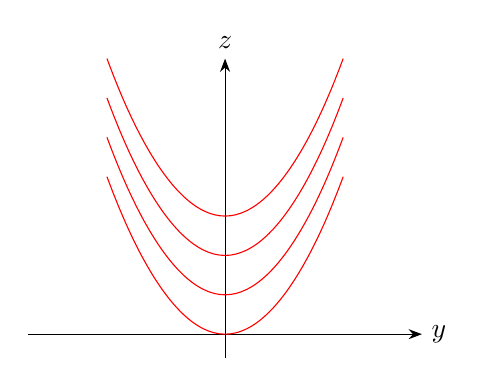
\begin{tikzpicture}[=>stealth]
\draw[-Stealth](-2.5,0)--(2.5,0)node[right]{$y$};
\draw[-Stealth](0,-0.3)--(0,3.5)node[above]{$z$};
\draw[red](0,0)parabola(1.5,2)
(0,0)parabola(-1.5,2)
(0,0.5)parabola(1.5,2.5)
(0,0.5)parabola(-1.5,2.5)
(0,1)parabola(1.5,3)
(0,1)parabola(-1.5,3)
(0,1.5)parabola(1.5,3.5)
(0,1.5)parabola(-1.5,3.5);
\end{tikzpicture}
\end{figure}

The trace in the plane $y = k$ is $z = 4x^2 + k^2$, again a parabola, narrower
since the coefficient of $x^2$ is larger; $y = 0$ gives $z = 4x^2$.

\begin{figure}[H]
\centering
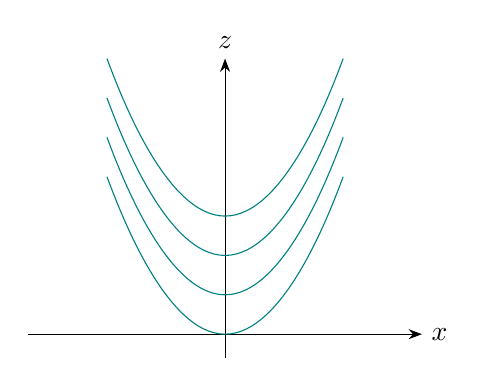
\begin{tikzpicture}[=>stealth]
\draw[-Stealth](-2.5,0)--(2.5,0)node[right]{$x$};
\draw[-Stealth](0,-0.3)--(0,3.5)node[above]{$z$};
\draw[teal](0,0)parabola(1.5,2)
(0,0)parabola(-1.5,2)
(0,0.5)parabola(1.5,2.5)
(0,0.5)parabola(-1.5,2.5)
(0,1)parabola(1.5,3)
(0,1)parabola(-1.5,3)
(0,1.5)parabola(1.5,3.5)
(0,1.5)parabola(-1.5,3.5);
\end{tikzpicture}
\end{figure}

The trace in the plane $z = k$ is $4x^2 + y^2 = k$: for $k>0$ an ellipse, with
semi-axes $\frac{\sqrt k}{2}$ and $\sqrt k$; for $k = 0$ the single point $(0,0)$;
and for $k<0$ nothing, so the surface lies on and above the $xy$-plane.

\begin{figure}[H]
\centering
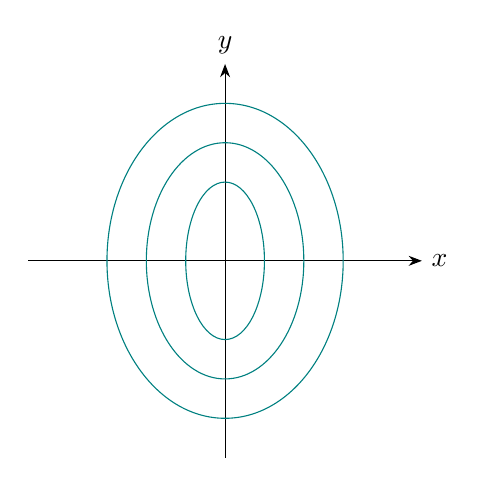
\begin{tikzpicture}[=>stealth]
\draw[-Stealth](-2.5,0)--(2.5,0)node[right]{$x$};
\draw[-Stealth](0,-2.5)--(0,2.5)node[above]{$y$};
\draw[teal](0,0)ellipse[x radius = 0.5cm, y radius=1cm]
(0,0)ellipse [x radius = 1cm, y radius = 1.5cm]
(0,0) ellipse [ x radius = 1.5cm , y radius = 2cm];
\end{tikzpicture}
\end{figure}

Horizontal ellipses and vertical parabolas together describe an \emph{elliptic
paraboloid}, a bowl opening upward along the $z$-axis.

\begin{figure}[H]
\centering
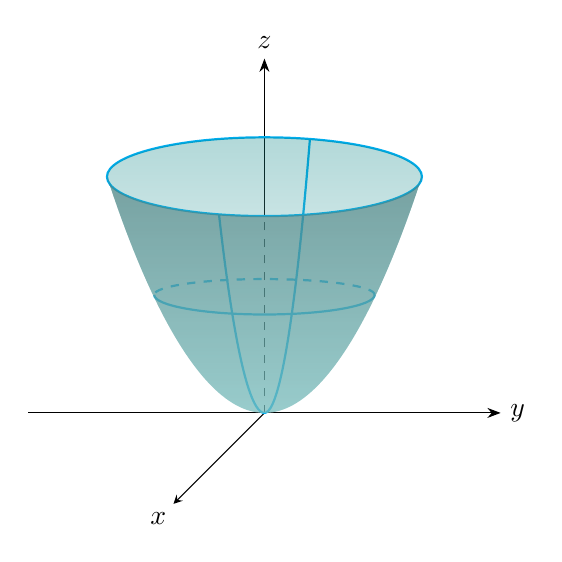
\begin{tikzpicture}[=>stealth]
\draw[-Stealth](-3,0,0)--(3,0,0)node[right]{$y$};
\draw[-Stealth](0,2.5,0)--(0,4.5,0)node[above]{$z$};
\draw[-stealth](0,0,0)--(0,0,3);
\draw(0,0,3.5)node[]{$x$};
\draw[dashed](0,0,0)--(0,2.5,0);
%\draw(0,0)parabola(2,3)
%(0,0)parabola(-2,3);
\draw[cyan,thick](2,3)arc(0:360:2cm and 0.5cm)
(0,0,0)parabola(0,3.1,1.5)
(0,0,0)parabola(0,2.9,-1.5)
(-1.4,1.5)arc(180:360:1.4cm and 0.25cm);
\draw[dashed,thick,cyan](1.4,1.5)arc(0:180:1.4cm and 0.2cm);
\shade[top color=teal,opacity=0.3](2,3)arc(0:180:2cm and 0.5cm)--(-2,3)parabola[bend at end](0,0)--(0,0)parabola(2,3)--cycle;
\shade[top color=teal,opacity=0.4](-2,3)arc(180:360:2cm and 0.5cm)--(2,3)parabola[bend at end](0,0)--(0,0)parabola(-2,3)--cycle;
\shade[bottom color=teal,opacity=0.4](-2,3)arc(180:360:2cm and 0.5cm)--(2,3)parabola[bend at end](0,0)--(0,0)parabola(-2,3)--cycle;
\end{tikzpicture}
\end{figure}
\end{solution}

The six non-degenerate quadric surfaces with centre or vertex at the origin, in
standard position, are listed below; in each case the axis of the surface is the
$z$-axis, and the roles of the variables can be permuted.
\begin{center}
\begin{tabular}{lll}
\hline
Surface & Equation & Horizontal traces ($z = k$)\\
\hline
Ellipsoid & $\frac{x^2}{a^2} + \frac{y^2}{b^2} + \frac{z^2}{c^2} = 1$ & ellipses, for
$|k|<c$\\[1ex]
Elliptic paraboloid & $\frac{z}{c} = \frac{x^2}{a^2} + \frac{y^2}{b^2}$ & ellipses\\[1ex]
Hyperbolic paraboloid & $\frac{z}{c} = \frac{x^2}{a^2} - \frac{y^2}{b^2}$ & hyperbolas\\[1ex]
Cone & $\frac{z^2}{c^2} = \frac{x^2}{a^2} + \frac{y^2}{b^2}$ & ellipses\\[1ex]
Hyperboloid of one sheet & $\frac{x^2}{a^2} + \frac{y^2}{b^2} - \frac{z^2}{c^2} = 1$
& ellipses, for every $k$\\[1ex]
Hyperboloid of two sheets & $-\frac{x^2}{a^2} - \frac{y^2}{b^2} + \frac{z^2}{c^2} =
1$ & ellipses, for $|k|>c$\\
\hline
\end{tabular}
\end{center}
A useful rule: the number of minus signs on the left of a centred equation
equal to $1$ is the number of sheets, and the variable whose square has the odd
sign out is the axis.

\begin{exa}
\label{ex:ellipsoid}
Sketch the quadric surface
\[ x^2 + \frac{y^2}{9} + \frac{z^2}{4} =1 .\]
\end{exa}

\begin{solution}
The trace in the plane $x = k$ is
\[\frac{y^2}{9}+ \frac{z^2}{4} = 1 -k^2 ,\]
an ellipse when $k^2<1$, a point when $k = \pm 1$, and empty when $|k|>1$. The
traces $y = k$ are the ellipses $x^2 + \frac{z^2}{4} = 1-\frac{k^2}{9}$ for
$|k|<3$, and the traces $z = k$ are the ellipses
$x^2 + \frac{y^2}{9} = 1- \frac{k^2}{4}$ for $|k|<2$. All traces are ellipses,
so the surface is an \emph{ellipsoid}, meeting the axes at $(\pm 1,0,0)$,
$(0,\pm 3,0)$ and $(0,0,\pm 2)$.

\begin{figure}[H]
\centering
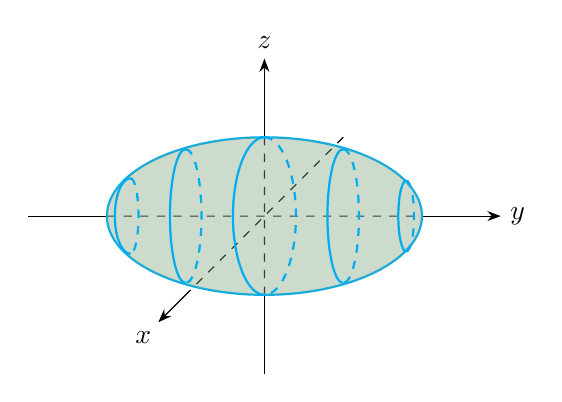
\begin{tikzpicture}[=>stealth]
\draw[-Stealth](2,0,0)--(3,0,0)node[right]{$y$};
\draw[-Stealth](0,1,0)--(0,2,0)node[above]{$z$};
\draw[-Stealth](0,0,2.6)--(0,0,3.5);
\draw[dashed](-2,0,0)--(2,0,0)
(0,-1,0)--(0,1,0)
(0,0,-2.6)--(0,0,2.6);
\draw(0,0,4)node[]{$x$}
(-3,0,0)--(-2,0,0)
(0,-2,0)--(0,-1,0);
\draw[thick,cyan](2,0)arc(0:360:2cm and 1cm);
\path[fill=cyan!50!orange,opacity=0.4](2,0)arc(0:360:2cm and 1cm);
\draw[dashed,thick,cyan](0,1)arc(90:-90:0.4cm and 1cm)
(1,0.85)arc(90:-90:0.2cm and 0.85cm)
(-1,0.85)arc(90:-90:0.2cm and 0.85cm)
(1.8,0.45)arc(90:-90:0.1cm and 0.45cm)
(-1.7,0.48)arc(90:-90:0.1cm and 0.48cm);
\draw[thick,cyan](0,1)arc(90:270:0.4cm and 1cm)
(1,0.85)arc(90:270:0.2cm and 0.85cm)
(-1,0.85)arc(90:270:0.2cm and 0.85cm)
(1.8,0.45)arc(90:270:0.1cm and 0.45cm)
(-1.7,0.48)arc(90:270:0.2cm and 0.48cm);
\end{tikzpicture}
\end{figure}
\end{solution}

\begin{exa}
\label{ex:classify}
Classify the quadric surface $x^2 + 2z^2 - 6x -y + 10 =0$.
\end{exa}

\begin{solution}
Complete the square in $x$:
\[(x^2 -6x + 9) + 2z^2 -y + 10 -9 =0,\qquad\text{that is}\qquad y-1 = (x-3)^2 +
2z^2 .\]
With $X = x - 3$, $Y = y - 1$, $Z = z$, this is $Y = X^2 + 2Z^2$, an elliptic
paraboloid with vertex $(3,1,0)$ whose axis is the line through the vertex
parallel to the $y$-axis. It opens in the direction of increasing $y$: the
traces $y = k$ are the ellipses $(x-3)^2 + 2z^2 = k - 1$ for $k>1$.

\begin{figure}[H]
\centering
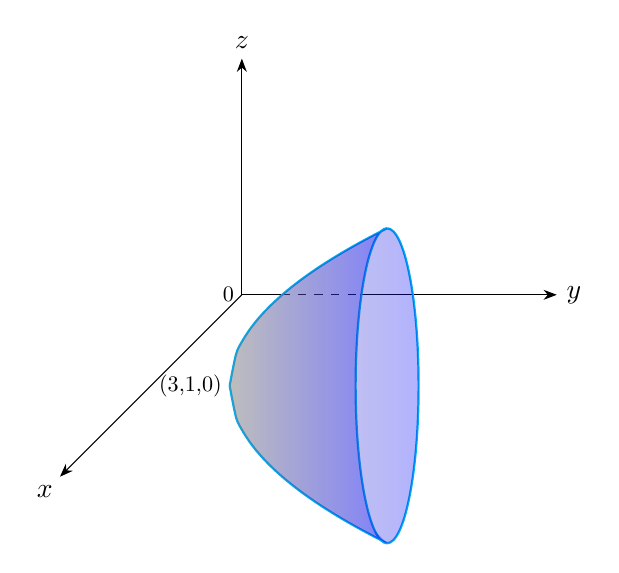
\begin{tikzpicture}[=>stealth]
\draw[-Stealth](0.5,0,-3)--(3,0,-3)node[right]{$y$};
\draw[-Stealth](-1,0,-3)--(-1,3,-3)node[above]{$z$};
\draw[-Stealth](-1,0,-3)--(-1,0,3);
\draw(-1,0,3.5)node[]{$x$}
(-1,0,-3)--(-0.5,0,-3)
(-1,0,-3)node[left,scale=0.8]{0}
(0,0,0)node[left,scale=0.8]{(3,1,0)};
\draw[dashed](-0.5,0,-3)--(0.5,0,-3);
\draw[smooth,domain=0:2,variable=\x,thick,cyan]plot(\x,{sqrt(2*\x)});
\draw[smooth,domain=0:2,variable=\x,thick,cyan]plot(\x,{-sqrt(2*\x)});
\draw[cyan,thick](2,2)arc(90:450:0.4cm and 2cm);
\shade[right color=blue,opacity=0.3,smooth,domain=0:2,variable=\x]plot(\x,{sqrt(2*\x)})--(2,2)arc(90:-90:0.4cm and 2cm)--plot(\x,{-sqrt(2*\x)})--cycle;
\shade[right color=blue,opacity=0.3,smooth,domain=0:2,variable=\x]plot(\x,{sqrt(2*\x)})--(2,2)arc(90:270:0.4cm and 2cm)--plot(\x,{-sqrt(2*\x)})--cycle;
\end{tikzpicture}
\end{figure}
\end{solution}

\begin{exe}
\label{exe:quadrics}
Use traces to identify and sketch the graphs of
\begin{enumerate}
\item $16x^2 - 9y^2 + 36z^2 = 144$;

\item $y^2 + 4z^2 =x$.
\end{enumerate}

\textbf{Answer:} (1) Dividing by $144$, $\frac{x^2}{9} - \frac{y^2}{16} +
\frac{z^2}{4} = 1$, a hyperboloid of one sheet with axis the $y$-axis (one minus
sign); its traces $y = k$ are ellipses for every $k$. (2) An elliptic paraboloid
with vertex at the origin, opening along the positive $x$-axis; its traces
$x = k>0$ are the ellipses $y^2 + 4z^2 = k$.
\end{exe}

\begin{exa}
\label{ex:saddlesurface}
Identify the surface $z = y^2 - x^2$ and describe its traces.
\end{exa}

\begin{solution}
The traces $x = k$ are the parabolas $z = y^2 - k^2$, opening upward; the traces
$y = k$ are the parabolas $z = k^2 - x^2$, opening downward; and the traces
$z = k$ are the hyperbolas $y^2 - x^2 = k$, which degenerate to the pair of lines
$y = \pm x$ when $k = 0$. The surface is a \emph{hyperbolic paraboloid}. Near the
origin it rises along the $y$-axis and falls along the $x$-axis: the saddle
surface of the saddle point in Example~\ref{ex:saddle}.
\end{solution}

\begin{exa}
\label{ex:hyperboloidcompleting}
Identify the surface $4x^2 - y^2 + 2z^2 + 4 = 0$.
\end{exa}

\begin{solution}
Dividing by $-4$,
\[-x^2 + \frac{y^2}{4} - \frac{z^2}{2} = 1 .\]
Two minus signs, with $y^2$ the odd one out: a hyperboloid of two sheets with
axis the $y$-axis. The traces $y = k$ are $x^2 + \frac{z^2}{2} =
\frac{k^2}{4} - 1$, ellipses when $|k|>2$ and empty when $|k|<2$, so the two
sheets lie in $y\geq 2$ and $y\leq -2$.
\end{solution}


{\color[wave]{485}\subsection{Surface of Revolution}}

A \emph{surface of revolution} is obtained by revolving a plane curve $C$ about a
line in its plane, the \emph{axis of revolution}. Each point of $C$ traces out a
circle centred on the axis and perpendicular to it.

\begin{figure}[H]
\centering
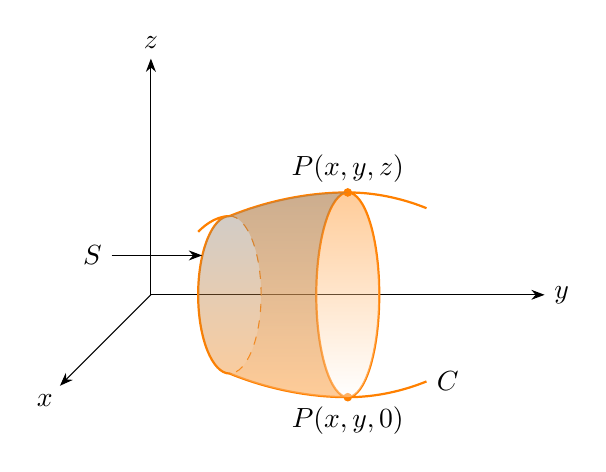
\begin{tikzpicture}[=>stealth]
\draw[-Stealth](0,0,0)--(5,0,0)node[right]{$y$};
\draw[-Stealth](0,0,0)--(0,3,0)node[above]{$z$};
\draw[-Stealth](0,0,0)--(0,0,3);
\draw(0,0,3.5)node[]{$x$};
\draw[orange,thick](2.5,1.3)arc(90:450:0.4cm and 1.3cm)
(1,1)arc(90:270:0.4cm and 1cm)
(1,1)parabola[bend at end](2.5,1.3)
(2.5,1.3)parabola(3.5,1.1)
(1,1)parabola(0.6,0.8)
(1,-1)parabola[bend at end](2.5,-1.3)
(2.5,-1.3)parabola(3.5,-1.1)node[right,black]{$C$};
\draw[-Stealth](-0.5,0.5)--(0.65,0.5);
\draw[dashed,orange](1,1)arc(90:-90:0.4cm and 1cm);
\draw(2.5,1.3)node[shape=circle,fill=orange,draw=orange,scale=0.01cm]{}
(2.5,-1.3)node[shape=circle,fill=orange,draw=orange,scale=0.01cm]{}
(2.5,1.3)node[above]{$P(x,y,z)$}
(2.5,-1.3)node[below]{$P(x,y,0)$}
(-0.5,0.5)node[left]{$S$};
\shade[top color=orange,opacity=0.4](2.5,1.3)arc(90:-90:0.4cm and 1.3cm)--(2.5,-1.3)--(2.5,-1.3)parabola(1,-1)--(1,-1)arc(270:450:0.4cm and 1cm)--(1,1)--(1,1)parabola[bend at end](2.5,1.3)--cycle;
\shade[bottom color=orange, opacity=0.4](2.5,1.3)arc(90:270:0.4cm and 1.3cm)--(2.5,-1.3)--(2.5,-1.3)parabola(1,-1)--(1,-1)arc(-90:-270:0.4cm and 1cm)--(1,1)--(1,1)parabola[bend at end](2.5,1.3)--cycle;
\end{tikzpicture}
\end{figure}

Let $C$ be the curve $f(y,z) = 0$ in the $yz$-plane, with $y\geq 0$ on $C$, and
revolve it about the $z$-axis. A point $P(x,y,z)$ lies on the resulting surface
$S$ exactly when its distance from the $z$-axis, $\sqrt{x^2 + y^2}$, is the
$y$-coordinate of a point of $C$ at the same height $z$. Hence
\[P(x,y,z)\ \text{lies on}\ S \iff f\left(\sqrt{x^2 + y^2},\, z\right) = 0 .\]
To find an equation for $S$, replace the coordinate measuring distance from the
axis by the distance $\sqrt{x^2 + y^2}$ from the axis, and leave the coordinate
along the axis unchanged. The same rule applies to any axis:
\begin{enumerate}
\item[$-$] about the $z$-axis, $f(y,z) = 0$ becomes
$f\left(\sqrt{x^2+y^2},\,z\right) = 0$;
\item[$-$] about the $y$-axis, $f(x,y) = 0$ becomes
$f\left(\sqrt{x^2+z^2},\,y\right) = 0$;
\item[$-$] about the $x$-axis, $f(x,y) = 0$ becomes
$f\left(x,\,\sqrt{y^2+z^2}\right) = 0$.
\end{enumerate}
If $C$ has points on both sides of the axis, replace the distance coordinate by
$\pm\sqrt{\cdots}$; when it appears only squared, as is usual, the sign does not
matter.

\begin{exa}
\label{ex:revolveellipse}
The ellipse $9x^2 + 4y^2 = 36$ in the $xy$-plane is revolved about the $y$-axis.
Find an equation for the resulting surface.

\begin{figure}[H]
\centering
\begin{tikzpicture}[=>stealth]
\draw[-Stealth](-2,0)--(2,0)node[right]{$x$};
\draw[-Stealth](0,-2)--(0,2)node[above]{$y$};
\draw[thick,cyan](0,0)ellipse[x radius = 0.8cm, y radius = 1.6cm];
\end{tikzpicture}
\end{figure}

Revolving about the $y$-axis, $y$ is unchanged and $x$ is replaced by
$\sqrt{x^2 + z^2}$:
\[9\left(\sqrt{x^2 + z^2}\right)^2 + 4y^2 = 36,\qquad\text{that is}\qquad 9x^2 +
4y^2 + 9z^2 = 36 .\]
The surface is an ellipsoid with circular cross-sections $y = k$, an ellipsoid
\emph{of revolution}.
\end{exa}

\begin{exa}
\label{ex:generating}
Find a generating curve and the axis of revolution for the surface
$x^2 + 3y^2 + z^2 = 9$.
\end{exa}

\begin{solution}
The coefficients of $x^2$ and $z^2$ are equal, so write
\[x^2 + z^2 = 9 - 3y^2 .\]
The left side is the square of the distance from the $y$-axis, so the surface is
obtained by revolution about the $y$-axis. A generating curve is the trace in
any plane through the axis: for example the ellipse $x^2 + 3y^2 = 9$ in the
$xy$-plane (with $z = 0$), or the ellipse $3y^2 + z^2 = 9$ in the $yz$-plane
(with $x = 0$).
\end{solution}

\begin{exa}
\label{ex:revolveline}
Find the surface obtained by revolving the line $z = 2y$, $y\geq 0$, in the
$yz$-plane about the $z$-axis.
\end{exa}

\begin{solution}
Replace $y$ by $\sqrt{x^2 + y^2}$: $z = 2\sqrt{x^2 + y^2}$, or, squaring,
$z^2 = 4(x^2 + y^2)$ with $z\geq 0$. It is the upper half of a circular cone with
vertex at the origin, the cone of the table above with $a = b = 1$, $c = 2$.
\end{solution}

\begin{exa}
\label{ex:torus}
The circle $(y - 3)^2 + z^2 = 1$ in the $yz$-plane is revolved about the
$z$-axis. Find an equation for the surface, a \emph{torus}.
\end{exa}

\begin{solution}
The circle lies in $y\geq 2$, so replacing $y$ by $\sqrt{x^2 + y^2}$ gives
\[\left(\sqrt{x^2 + y^2} - 3\right)^2 + z^2 = 1 .\]
This is not a quadric: clearing the root gives an equation of degree four,
$(x^2 + y^2 + z^2 + 8)^2 = 36(x^2 + y^2)$.
\end{solution}

{\color[wave]{485}\subsection{Cylindrical and Spherical Coordinates}}

In three dimensions there are two coordinate systems, besides the rectangular
one, that give simple descriptions of commonly occurring surfaces and solids.

\subhead{Cylindrical Coordinates}

A point $P$ is given the \emph{cylindrical coordinates} $(r,\theta,z)$, where
$(r,\theta)$ are polar coordinates of its projection onto the $xy$-plane and $z$
is its height.

\begin{figure}[H]
\centering
\begin{tikzpicture}[=>stealth]
\draw[-Stealth](-0.5,0,0)--(4,0,0)node[right]{$y$};
\draw[-Stealth](0,-0.5,0)--(0,3,0)node[above]{$z$};
\draw[-Stealth](0,0,-0.5)--(0,0,4);
\draw(0,0,4.5)node[]{$x$}
(-0.3,0,0)node[above]{0}
(3,0,3)node[shape=circle,fill=red,scale=0.01cm]{}
(3,3,3)node[shape=circle,fill=red,scale=0.01cm]{}
(3,3,3)node[above,scale=0.9]{$P(r,\theta, z)$}
(3,0,3)node[right,scale=0.9]{$(r,\theta,0)$}
(3,1.5,3)node[right]{$z$}
(1.5,0,1.5)node[above]{$r$};
\draw[red](0,0,0)--(3,0,3);
\draw[red](3,0,3)--(3,3,3);
\coordinate (a) at (0,0,0.5);
\coordinate (b) at (0,0,0);
\coordinate (c) at (0.5,0,0.5);
\draw
pic[draw = red, angle radius = 0.5cm, ->, "$\theta$", angle eccentricity=1.4]{angle = a--b--c};
\draw(2.8,0,2.8)--(2.8,0.2,2.8)--(3,0.2,3)
(0,0,2.7)--(0.3,0,2.7)--(0.3,0,3)
(2.7,0,0)--(2.7,0,0.3)--(3,0,0.3);
\draw[dashed,cyan](0,0,3)--(2.97,0,3)
(3,0,2.97)--(3,0,0);
\end{tikzpicture}
\end{figure}

To convert from cylindrical to rectangular coordinates,
\[x = r\cos \theta ,\qquad  y = r\sin \theta ,\qquad  z =z ,\]
and from rectangular to cylindrical,
\[r^2 = x^2 + y^2 , \qquad  \tan \theta = \frac{y}{x} ,\qquad  z =z ,\]
with $\theta$ chosen in the quadrant of $(x,y)$. Cylindrical coordinates suit
problems with symmetry about an axis, which is then taken as the $z$-axis: the
cylinder of radius $a$ about the $z$-axis is simply $r = a$.

\begin{exa}
\label{ex:conecyl}
Describe the surface whose equation in cylindrical coordinates is $z = r$.
\end{exa}

\begin{solution}
At each point $z = r\geq 0$, and squaring gives $z^2 = r^2 = x^2 + y^2$. So the
surface is the part of the circular cone $z^2 = x^2 + y^2$ with $z\geq 0$: a cone
with vertex at the origin, axis the $z$-axis, opening upward at $45^\circ$ to the
axis.
\end{solution}

\begin{exa}
\label{ex:ellipsoidcyl}
Find an equation in cylindrical coordinates for the ellipsoid
$4x^2 + 4y^2 + z^2 =1$.
\end{exa}

\begin{solution}
Since $x^2 + y^2 = r^2$,
\[4r^2 + z^2 =1,\qquad\text{or}\qquad z^2 = 1 - 4r^2 .\]
The absence of $\theta$ reflects the symmetry of the ellipsoid about the
$z$-axis.
\end{solution}

\subhead{Spherical Coordinates}

The \emph{spherical coordinates} $(\rho, \theta, \phi)$ of a point $P$ in space
are shown below.

\begin{figure}[H]
\centering
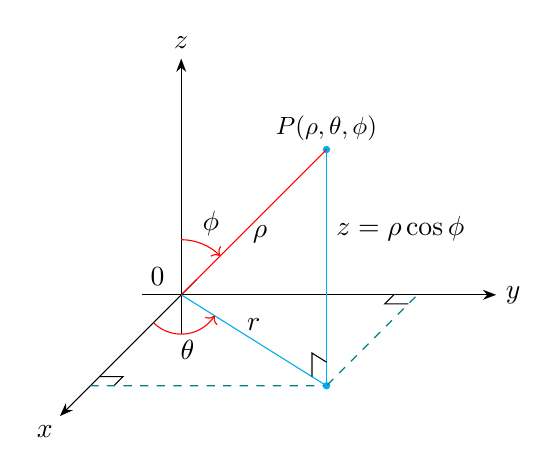
\begin{tikzpicture}[=>stealth]
\draw[-Stealth](-0.5,0,0)--(4,0,0)node[right]{$y$};
\draw[-Stealth](0,-0.5,0)--(0,3,0)node[above]{$z$};
\draw[-Stealth](0,0,-0.5)--(0,0,4);
\draw(0,0,4.5)node[]{$x$}
(-0.3,0,0)node[above]{0}
(3,0,3)node[shape=circle,fill=cyan,scale=0.01cm]{}
(3,3,3)node[shape=circle,fill=cyan,scale=0.01cm]{}
(3,3,3)node[above,scale=0.9]{$P(\rho,\theta, \phi)$}
(3,2,3)node[right]{$z=\rho \cos \phi$}
(1.5,0,1.5)node[above]{$r$}
(1,1,0)node[below]{$\rho$};
\draw[cyan](0,0,0)--(3,0,3);
\draw[cyan](3,0,3)--(3,3,3);
\coordinate (a) at (0,0,0.5);
\coordinate (b) at (0,0,0);
\coordinate (c) at (0.5,0,0.5);
\draw
pic[draw = red, angle radius = 0.5cm, ->, "$\theta$", angle eccentricity=1.4]{angle = a--b--c};
\draw(2.7,0,2.7)--(2.7,0.3,2.7)--(3,0.3,3)
(0,0,2.7)--(0.3,0,2.7)--(0.3,0,3)
(2.7,0,0)--(2.7,0,0.3)--(3,0,0.3);
\draw[dashed,teal](0,0,3)--(2.97,0,3)
(3,0,2.97)--(3,0,0);
\draw[red](0,0,0)--(3,3,3);
\coordinate (A) at (0.5,0.5,0);
\coordinate (B) at (0,0.5,0);
\draw
pic[draw = red, angle radius = 0.7cm,<-, "$\phi$", angle eccentricity =1.4]{angle=A--b--B};
\end{tikzpicture}
\end{figure}

Here $\rho = |OP|$ is the distance from the origin to $P$, $\theta$ is the same
angle as in cylindrical coordinates, and $\phi$ is the angle between the positive
$z$-axis and the line segment $OP$, with
\[\rho\geq 0 , \qquad  0\leq \theta < 2\pi , \qquad  0 \leq \phi \leq \pi .\]
The triangle formed by $O$, $P$ and the projection of $P$ on the $z$-axis is
right-angled, with hypotenuse $\rho$ and angle $\phi$ at $O$, so
$z = \rho\cos\phi$ and the distance from the $z$-axis is $r = \rho\sin\phi$.
Combining with $x = r\cos\theta$ and $y = r\sin\theta$,
\[x = \rho \sin \phi \cos \theta ,\qquad y =\rho \sin \phi \sin \theta ,\qquad z =
\rho \cos \phi ,\qquad \rho^2 = x^2 + y^2 + z^2 .\]
The sphere of radius $a$ about the origin is $\rho = a$, the cone $z^2 = x^2 +
y^2$ with $z\geq 0$ is $\phi = \frac{\pi}{4}$, and the half-plane through the
$z$-axis at angle $\theta_0$ is $\theta = \theta_0$.

\begin{exa}
\label{ex:hyperboloidsph}
Find an equation in spherical coordinates for $x^2 -y^2 -z^2 = 1$.
\end{exa}

\begin{solution}
Substituting,
\[\rho^2\sin^2\phi \cos^2 \theta - \rho^2 \sin^2\phi \sin^2\theta -
\rho^2\cos^2\phi = 1 .\]
Since $\cos^2\theta - \sin^2 \theta = \cos 2\theta$,
\[\rho^2\left(\sin^2\phi \cos2\theta - \cos^2\phi\right) =1 .\]
\end{solution}

\begin{exa}
\label{ex:spheresph}
Find a rectangular equation for the surface whose spherical equation is
$\rho = \sin \phi \sin \theta$.
\end{exa}

\begin{solution}
Multiply by $\rho$, so that the right side becomes a rectangular coordinate:
\[\rho^2 = \rho\sin\phi\sin\theta,\qquad\text{that is}\qquad x^2 + y^2 + z^2 = y
.\]
Completing the square,
\[x^2 + \left(y - \frac12\right)^2 + z^2 = \frac{1}{4},\]
the sphere with radius $\frac{1}{2}$ and centre $\left(0, \frac12,0\right)$.
(Multiplying by $\rho$ adds only the origin, which already lies on the sphere.)
\end{solution}

\begin{exa}
\label{ex:pointsph}
The point $\left( 2, \frac{\pi}{4}, \frac{\pi}{3}\right)$ is given in spherical
coordinates $(\rho,\theta,\phi)$. Find its rectangular coordinates.
\end{exa}

\begin{solution}
\begin{align*}
x & = \rho \sin \phi \cos \theta = 2 \sin \frac{\pi}{3}\cos \frac{\pi}{4} =
2\cdot \frac{\sqrt{3}}{2}\cdot \frac{1}{\sqrt{2}}=\sqrt{\frac{3}{2}},\\
y & = \rho \sin \phi \sin\theta = 2 \sin \frac{\pi}{3} \sin \frac{\pi}{4} =
\sqrt{\frac{3}{2}},\\
z & = \rho \cos \phi = 2\cos \frac{\pi}{3} = 1 .
\end{align*}
As a check, $x^2 + y^2 + z^2 = \frac32 + \frac32 + 1 = 4 = \rho^2$.
\end{solution}

\begin{exe}
\label{exe:tospherical}
Express the point $(0,2\sqrt{3},-2)$, given in rectangular coordinates, in
spherical coordinates.

\textbf{Answer:} $\rho = \sqrt{0 + 12 + 4} = 4$; $\cos\phi = \frac{z}{\rho} =
-\frac12$, so $\phi = \frac{2\pi}{3}$; and since $x = 0$ and $y>0$,
$\theta = \frac{\pi}{2}$. The point is $\left(4, \frac{\pi}{2},
\frac{2\pi}{3}\right)$.
\end{exe}

\begin{exa}
\label{ex:cyltosph}
Convert the cylindrical equation $r^2 + z^2 = 4z$ to spherical coordinates and
identify the surface.
\end{exa}

\begin{solution}
Since $r^2 + z^2 = \rho^2$ and $z = \rho\cos\phi$, the equation is
$\rho^2 = 4\rho\cos\phi$, that is $\rho = 4\cos\phi$ (together with the origin).
In rectangular form it is $x^2 + y^2 + (z-2)^2 = 4$, the sphere of radius $2$
centred at $(0,0,2)$, which touches the $xy$-plane at the origin.
\end{solution}

{\color[wave]{485}\subsection{Tangent Planes}}

Let $S$ be the surface $z = f(x,y)$ and $P(x_0,y_0,z_0)$ a point of $S$. The
vertical planes $y = y_0$ and $x = x_0$ cut $S$ in curves $C_1$ and $C_2$
through $P$, whose slopes at $P$ are $f_x(x_0,y_0)$ and $f_y(x_0,y_0)$.

\begin{figure}[H]
\centering
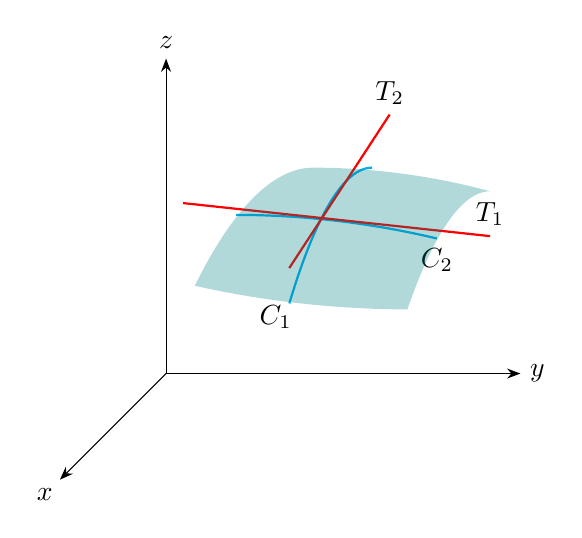
\begin{tikzpicture}[=>stealth]
\draw[-Stealth](0,0,-1)--(4.5,0,-1)node[right]{$y$};
\draw[-Stealth](0,0,-1)--(0,4,-1)node[above]{$z$};
\draw[-Stealth](0,0,-1)--(0,0,2.5);
\draw(0,0,3)node[]{$x$}
%(2.55,1.4)node[right]{$C_2$}
(1.45,1.1)node[right]{$C_1$};
%\draw[scale=1.5,teal](0.5,1)parabola[bend at end](1.5,2)
%(1.5,2)parabola(3,1.8)
%(3,1.8)parabola(2.3,0.8)
%(2.3,0.8)parabola(0.5,1);
\draw[scale=1.5,thick,cyan](1.3,0.85)parabola[bend at end](2,2)
(0.85,1.6)parabola(2.55,1.4)node[black,below]{$C_2$};
\draw[scale=1.5,thick,red](0.4,1.7)--(3,1.42)node[black,above]{$T_1$}
(1.3,1.15)--(2.15,2.45)node[black,above]{$T_2$};
\path[fill=teal,opacity=0.3,scale=1.5](0.5,1)parabola[bend at end](1.5,2)--(1.5,2)parabola(3,1.8)--(3,1.8)parabola(2.3,0.8)--(2.3,0.8)parabola(0.5,1)--cycle;
\end{tikzpicture}
\end{figure}

Let $T_1$ and $T_2$ be the tangent lines to $C_1$ and $C_2$ at $P$. The
\emph{tangent plane} to $S$ at $P$ is the plane that contains $T_1$ and $T_2$.
When $f$ is differentiable it contains the tangent lines at $P$ of every curve
in $S$ through $P$, and it is the graph of the linear approximation of
Definition~\ref{defn:differentiable}.

\subhead{Equation of Tangent Plane}

Suppose $f$ has continuous first partial derivatives. An equation of the tangent
plane to the surface $z = f(x,y)$ at the point $P(x_0, y_0, z_0)$ is
\[z -z_0 = f_x(x_0,y_0)(x-x_0) + f_y(x_0,y_0)(y-y_0) .\]
Indeed, the plane through $P$ with this equation contains $T_1$, since setting
$y = y_0$ leaves the line of slope $f_x(x_0,y_0)$ in the plane $y = y_0$, and
likewise it contains $T_2$.

\begin{exa}
\label{ex:tangentparaboloid}
Find the tangent plane to the elliptic paraboloid $z = 2x^2 + y^2$ at the point
$(1,1,3)$.
\end{exa}

\begin{solution}
With $f = 2x^2 + y^2$, $f_x = 4x$ and $f_y = 2y$, which are $4$ and $2$ at
$(1,1)$. So the tangent plane is
\[z - 3 = 4(x-1) + 2(y-1),\qquad\text{that is}\qquad z = 4x + 2y -3 .\]
\end{solution}

\begin{exa}
\label{ex:tangentexp}
Find the tangent plane to $z = xe^{xy}$ at $(1,0,1)$, and use it to approximate
$1.1e^{-0.11}$.
\end{exa}

\begin{solution}
$f_x = e^{xy} + xye^{xy}$ and $f_y = x^2e^{xy}$, which are $1$ and $1$ at
$(1,0)$. The tangent plane is $z = 1 + (x - 1) + y = x + y$. The point $(1.1,
-0.1)$ gives $f = 1.1e^{-0.11}$, approximated by $1.1 - 0.1 = 1$; the exact value
is $0.9854$.
\end{solution}

{\color[wave]{485}\subsection{Parametric Surfaces}}

A curve in space is described by a vector function of one parameter. A surface
needs two. Suppose that
\begin{equation}
\mathbf r(u,v) = x(u,v)\,\mathbf i + y(u,v)\,\mathbf j + z(u,v)\,\mathbf k
\label{eq:paramsurface}
\end{equation}
is a vector function defined on a region $D$ in the $uv$-plane. The set of
points $(x,y,z)$ in $\mathbb{R}^3$ with
\[x = x(u,v) ,\qquad  y = y(u,v) , \qquad  z = z(u,v) ,\]
as $(u,v)$ varies throughout $D$, is a \emph{parametric surface} $S$, and these
are its \emph{parametric equations}. As $(u,v)$ moves over $D$, the tip of the
position vector $\mathbf r(u,v)$ moves over $S$.

\begin{table}[H]
\centering
\begin{tabular}{cc}
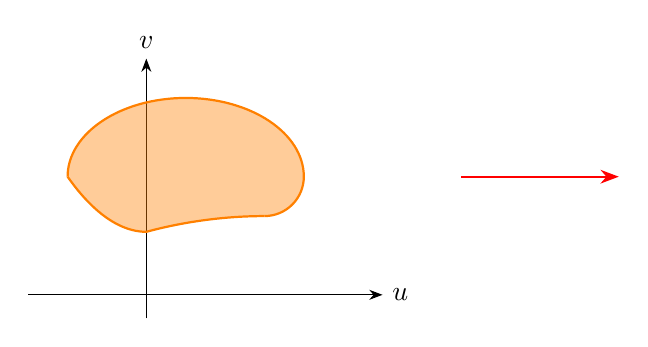
\begin{tikzpicture}[=>stealth]
\draw[-Stealth](-1.5,0)--(3,0)node[right]{$u$};
\draw[-Stealth](0,-0.3)--(0,3)node[above]{$v$};
\draw[thick,orange](2,1.5)arc(0:180:1.5cm and 1cm)
(2,1.5)arc(0:-90:0.5cm and 0.5cm);
%(-1,1.5)parabola[bend at end](0,1)
%(0,1)parabola(1,1.5)
%(1,1.5)parabola(1.5,1);
\draw[thick,orange](0,0.8)parabola[bend at  end](1.5,1)
(-1,1.5)parabola[bend at end](0,0.8);
%\path[fill=orange,opacity=0.4](2,1.5)arc(0:180:1.5cm and 1cm)--(-1,1.5)parabola[bend at end](0,1)--(0,1)parabola(1,1.5)--(1,1.5)parabola(1.5,1)--(1.5,1)arc(270:360:0.5cm and 0.5cm)--cycle;
\path[fill=orange,opacity=0.4](2,1.5)arc(0:180:1.5cm and 1cm)--(-1,1.5)parabola[bend at end](0,0.8)--(0,0.8)parabola[bend at end](1.5,1)--(1.5,1)arc(270:360:0.5cm and 0.5cm)--cycle;
\draw[thick,red,-Stealth](4,1.5)--(6,1.5);
\end{tikzpicture}
&
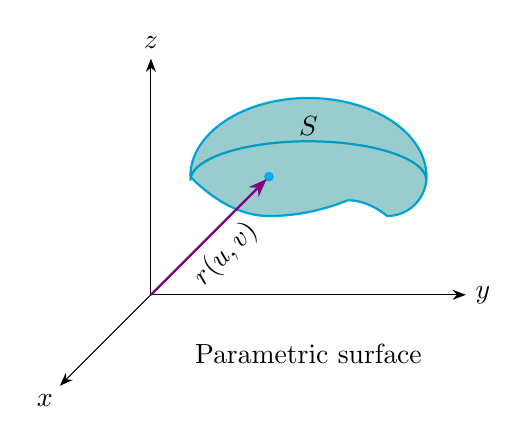
\begin{tikzpicture}[=>stealth]
\draw[-Stealth](0,0,0)--(4,0,0)node[right]{$y$};
\draw[-Stealth](0,0,0)--(0,3,0)node[above]{$z$};
\draw[-Stealth](0,0,0)--(0,0,3);
\draw(0,0,3.5)node[]{$x$};
\draw[thick,cyan](3.5,1.5)arc(0:180:1.5cm and 1cm)
(3.5,1.5)arc(0:-90:0.5cm and 0.5cm)
(0.5,1.5)parabola[bend at end](1.5,1)
(1.5,1)parabola(2.5,1.2)
(2.5,1.2)parabola(3,1)
(0.5,1.45)arc(180:0:1.5cm and 0.5cm);
\path[fill=teal,opacity=0.4](3.5,1.5)arc(0:180:1.5cm and 1cm)--(0.5,1.45)arc(180:0:1.5cm and 0.5cm)--cycle;
\path[fill=teal,opacity=0.4](0.5,1.45)arc(180:0:1.5cm and 0.5cm)--(3.5,1.5)arc(0:-90:0.5cm and 0.5cm)--(3,1)parabola[bend at end](2.5,1.2)--(2.5,1.2)parabola[bend at end](1.5,1)--(1.5,1)parabola(0.5,1.5)--cycle;
\draw(1.5,1.5)node[shape=circle,fill=cyan,scale=0.01cm,draw=cyan,thick]{}
(2,1.9)node[above]{$S$};
\draw[-Stealth,thick,violet](0,0)--node[below,black,sloped]{$r(u,v)$}(1.47,1.47);
\draw(2,-1)node[above]{Parametric surface};
\end{tikzpicture}\\
\end{tabular}
\end{table}

\begin{exa}
\label{ex:cylinderparam}
Identify and sketch the surface with vector equation
$\mathbf r(u,v) = 2\cos u\, \mathbf i + v\,\mathbf j + 2\sin u\, \mathbf k$.
\end{exa}

\begin{solution}
The parametric equations are $x = 2\cos u$, $y = v$, $z = 2\sin u$, so for every
point
\[x^2 + z^2 = 4\cos^2 u + 4\sin^2 u = 4 ,\]
while $y = v$ is unrestricted. The surface is the circular cylinder of radius
$2$ whose axis is the $y$-axis.

\begin{figure}[H]
\centering
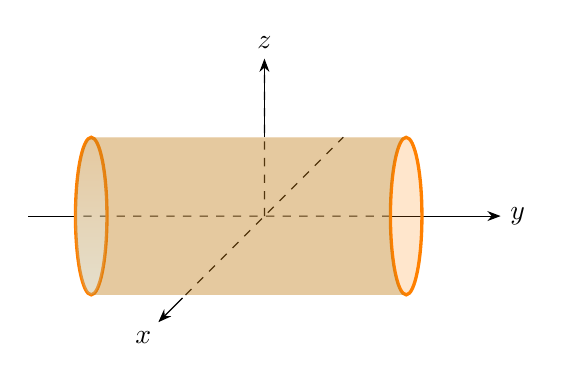
\begin{tikzpicture}[=>stealth]
\draw[-Stealth](1.6,0,0)--(3,0,0)node[right]{$y$};
\draw[-Stealth](0,1,0)--(0,2,0)node[above]{$z$};
\draw[-Stealth](0,0,2.7)--(0,0,3.5);
\draw(0,0,4)node[]{$x$}
(-3,0,0)--(-2.4,0,0);
\draw[dashed]((-2.3,0,0)--(1.6,0,0)
(0,0,0)--(0,1.9,0)
(0,0,2.6)--(0,0,-2.6);
\draw[very thick,orange](2,0,0)arc(0:360:0.2cm and 1cm);
\draw[very thick,orange](-2,0,0)arc(0:360:0.2cm and 1cm);
\path[fill=orange,opacity=0.2](1.8,1,0)arc(90:-90: 0.2cm and 1cm)--(1.8,-1,0)--(-2.2,-1,0)--(-2.2,-1,0)arc(-90:90:0.2cm and 1cm)--(-2.2,1,0)--cycle;
\path[fill=orange,opacity=0.2](-2.2,1,0)arc(90:270: 0.2cm and 1cm)--(-2.2,-1,0)--(1.8,-1,0)--(1.8,-1,0)arc(270:90:0.2cm and 1cm)--(1.8,1,0)--cycle;
\shade[top color=orange,opacity=0.2](-2,0,0)arc(0:360:0.2cm and 1cm);
%%
\path[fill=teal,opacity=0.1](-2.2,1,0)arc(90:270: 0.2cm and 1cm)--(-2.2,-1,0)--(1.8,-1,0)--(1.8,-1,0)arc(270:90:0.2cm and 1cm)--(1.8,1,0)--cycle;
\end{tikzpicture}
\end{figure}

If the parameters are restricted to $0\leq u \leq \frac{\pi}{2}$ and
$0 \leq v \leq 3$, then $x\geq 0$, $z \geq 0$ and $0\leq y \leq 3$, and the
surface is the quarter of the cylinder of length $3$ lying above the first
quadrant of the $xy$-plane.

\begin{figure}[H]
\centering
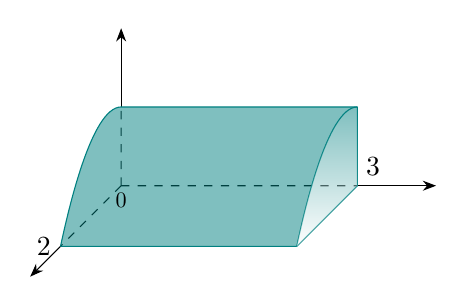
\begin{tikzpicture}[=>stealth]
\draw[-Stealth](3,0,0)--(4,0,0);
\draw[-Stealth](0,1,0)--(0,2,0);
\draw[-Stealth](0,0,2)--(0,0,3);
\draw[dashed](0,0,0)--(3,0,0)
(0,0,0)--(0,1,0)
(0,0,0)--(0,0,2);
\draw[teal](0,1,0)--(3,1,0)
(0,0,2)--(3,0,2)
(3,0,2)--(3,0,0)--(3,1,0);
\draw[teal](0,0,2)parabola[bend at end](0,1,0)
(3,0,2)parabola[bend at end](3,1,0);
\path[fill=teal,opacity=0.5](0,0,2)parabola[bend at end](0,1,0)--(3,1,0)parabola(3,0,2)--(0,0,2)--cycle;
\shade[top color=teal,opacity=0.5](3,1,0)parabola(3,0,2)--(3,0,0)--(3,1,0);
\draw(0,0,0)node[below,scale=0.8]{0}
(0,0,2)node[left]{2}
(3.2,0,0)node[above]{3};
\end{tikzpicture}
\end{figure}
\end{solution}

\begin{exa}
\label{ex:sphereparam}
Find a parametric representation of the sphere $x^2 + y^2 + z^2 = a^2$.
\end{exa}

\begin{solution}
The sphere is $\rho = a$ in spherical coordinates, so $\phi$ and $\theta$ serve
as parameters:
\[x = a\sin \phi \cos \theta , \qquad  y = a\sin \phi\sin \theta , \qquad  z =
a\cos \phi ,\]
that is,
\[\mathbf r(\phi, \theta) = a\sin \phi \cos \theta\, \mathbf i + a \sin \phi \sin
\theta\, \mathbf j + a\cos \phi \,\mathbf k ,\qquad (\phi,\theta)\in D =
[0,\pi]\times [0,2\pi] .\]
For the sphere of radius $9$, take $a = 9$.
\end{solution}

\begin{exa}
\label{ex:graphparam}
Show that every graph $z = f(x,y)$ is a parametric surface, and parametrise the
part of the paraboloid $z = x^2 + y^2$ below the plane $z = 4$ in two ways.
\end{exa}

\begin{solution}
Take $x$ and $y$ themselves as parameters: $\mathbf r(x,y) = x\,\mathbf i +
y\,\mathbf j + f(x,y)\,\mathbf k$. For the paraboloid this gives
$\mathbf r(x,y) = \langle x, y, x^2 + y^2\rangle$ on the disc $x^2 + y^2\leq 4$.
Alternatively, polar coordinates give
$\mathbf r(r,\theta) = \langle r\cos\theta, r\sin\theta, r^2\rangle$ on the
rectangle $0\leq r\leq 2$, $0\leq\theta\leq 2\pi$, whose parameter domain is
simpler.
\end{solution}

\begin{exa}
\label{ex:coneparam}
Find a parametric representation of the cone $z = \sqrt{x^2 + y^2}$ for
$0\leq z\leq 3$.
\end{exa}

\begin{solution}
In cylindrical coordinates the cone is $z = r$, so with $r$ and $\theta$ as
parameters,
\[\mathbf r(r,\theta) = \langle r\cos\theta,\ r\sin\theta,\ r\rangle ,\qquad
0\leq r\leq 3,\quad 0\leq\theta\leq 2\pi .\]
\end{solution}

{\color[wave]{485}\subsection{Tangent Planes To Parametric Surfaces}}

Let $S$ be the parametric surface traced out by
$\mathbf r(u,v) = x(u,v)\, \mathbf i + y(u,v)\,\mathbf j + z(u,v)\,\mathbf k$,
and $P_0$ the point with position vector $\mathbf r(u_0,v_0)$. Holding
$u = u_0$ fixed, $\mathbf r(u_0,v)$ is a vector function of the single
parameter $v$, and defines a curve $C_1$ lying on $S$. Its tangent vector at
$P_0$ is
\[\mathbf r_v = \frac{\partial x}{\partial v}(u_0,v_0)\,\mathbf i +
\frac{\partial y}{\partial v}(u_0,v_0)\,\mathbf j +\frac{\partial z}{\partial
v}(u_0,v_0)\,\mathbf k .\]

\begin{table}[H]
\centering
\begin{tabular}{cc}
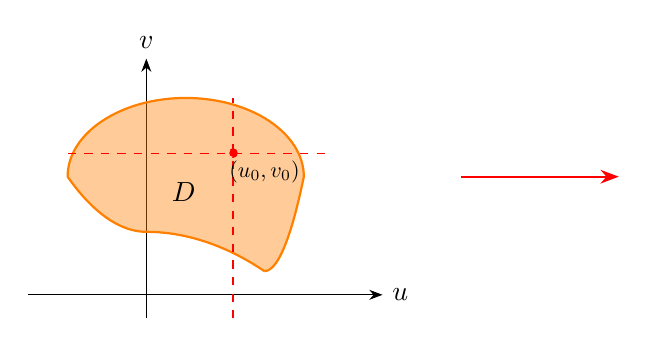
\begin{tikzpicture}[=>stealth]
\draw[-Stealth](-1.5,0)--(3,0)node[right]{$u$};
\draw[-Stealth](0,-0.3)--(0,3)node[above]{$v$};
\draw[thick,orange](2,1.5)arc(0:180:1.5cm and 1cm)
(0,0.8)parabola(1.5,0.3)
(1.5,0.3)parabola(2,1.5)
(-1,1.5)parabola[bend at end](0,0.8);
\path[fill=orange,opacity=0.4](2,1.5)arc(0:180:1.5cm and 1cm)--(-1,1.5)parabola[bend at end](0,0.8)--(0,0.8)parabola(1.5,0.3)--(1.5,0.3)parabola(2,1.5)--cycle;
\draw[thick,red,-Stealth](4,1.5)--(6,1.5);
\draw[dashed,red](1.1,-0.3)--(1.1,2.5)
(-1,1.8)--(2.3,1.8)
(1.1,1.8)node[shape=circle,fill=red,scale=0.01cm,draw=red,thick]{}
(0.2,1.3)node[right,black]{$D$}
(1.5,1.8)node[below,black,scale=0.8]{$(u_0,v_0)$};
\end{tikzpicture}
&
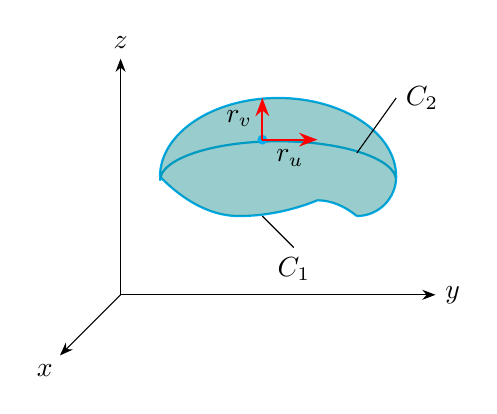
\begin{tikzpicture}[=>stealth]
\draw[-Stealth](0,0,0)--(4,0,0)node[right]{$y$};
\draw[-Stealth](0,0,0)--(0,3,0)node[above]{$z$};
\draw[-Stealth](0,0,0)--(0,0,2);
\draw(0,0,2.5)node[]{$x$};
\draw[thick,cyan](3.5,1.5)arc(0:180:1.5cm and 1cm)
(3.5,1.5)arc(0:-90:0.5cm and 0.5cm)
(0.5,1.5)parabola[bend at end](1.5,1)
(1.5,1)parabola(2.5,1.2)
(2.5,1.2)parabola(3,1)
(0.5,1.45)arc(180:0:1.5cm and 0.5cm);
\path[fill=teal,opacity=0.4](3.5,1.5)arc(0:180:1.5cm and 1cm)--(0.5,1.45)arc(180:0:1.5cm and 0.5cm)--cycle;
\path[fill=teal,opacity=0.4](0.5,1.45)arc(180:0:1.5cm and 0.5cm)--(3.5,1.5)arc(0:-90:0.5cm and 0.5cm)--(3,1)parabola[bend at end](2.5,1.2)--(2.5,1.2)parabola[bend at end](1.5,1)--(1.5,1)parabola(0.5,1.5)--cycle;
\draw(1.8,1.97)node[shape=circle,fill=cyan,scale=0.01cm,draw=cyan,thick]{};
\draw[-Stealth,thick,red](1.8,1.97)--node[below,black,sloped]{$r_u$}(2.5,1.97);
\draw[-Stealth,thick,red](1.8,1.97)--node[left,black,]{$r_v$}(1.8,2.5);
\draw(1.8,1)--(2.2,0.6)node[below]{$C_1$}
(3,1.8)--(3.5,2.5)node[right]{$C_2$};
\end{tikzpicture}\\
\end{tabular}
\end{table}

Similarly, holding $v = v_0$ fixed gives a curve $C_2$, given by
$\mathbf r(u,v_0)$, lying on $S$, with tangent vector
\[\mathbf r_u = \frac{\partial x}{\partial u}(u_0,v_0)\,\mathbf i +
\frac{\partial y}{\partial u}(u_0,v_0)\,\mathbf j +\frac{\partial z}{\partial
u}(u_0,v_0)\,\mathbf k .\]
If $\mathbf r_u \times \mathbf r_v \neq \mathbf 0$ at $(u_0,v_0)$, the surface is
\emph{smooth} there. For a smooth surface the \emph{tangent plane} at $P_0$ is
the plane through $P_0$ that contains the tangent vectors $\mathbf r_u$ and
$\mathbf r_v$, and $\mathbf r_u \times \mathbf r_v$ is a normal vector to it.

\begin{exa}
\label{ex:tangentparam}
Find the tangent plane to the surface with parametric equations
\[x =u^2 ,\qquad  y = v^2 , \qquad  z = u + 2v\]
at the point $(1,1,3)$.
\end{exa}

\begin{solution}
With $\mathbf r(u,v) = u^2 \,\mathbf i + v^2\,\mathbf j + (u + 2v)\,\mathbf k$,
\[\mathbf r_u = 2u\,\mathbf i + \mathbf k ,\qquad \mathbf r_v = 2v\,\mathbf j+
2\,\mathbf k ,\]
and a normal vector is
\[\mathbf r_u  \times \mathbf r_v = \begin{vmatrix}
\mathbf i & \mathbf j & \mathbf k\\
2u & 0 & 1\\
0 & 2v & 2
\end{vmatrix} = -2v\,\mathbf i -4u\,\mathbf j + 4uv\,\mathbf k .\]
The point $(1,1,3)$ corresponds to $u = 1$, $v = 1$, where the normal is
$\langle -2, -4, 4\rangle$. So the tangent plane is
\[-2(x-1) -4(y-1) + 4(z-3) =0,\qquad\text{that is}\qquad  x+ 2y -2z + 3 = 0 .\]
\end{solution}

\begin{exa}
\label{ex:tangentsphereparam}
Find the tangent plane to the sphere $\mathbf r(\phi,\theta) = \langle
2\sin\phi\cos\theta, 2\sin\phi\sin\theta, 2\cos\phi\rangle$ at the point with
$\phi = \frac{\pi}{4}$, $\theta = 0$.
\end{exa}

\begin{solution}
The point is $(\sqrt2, 0, \sqrt2)$. Differentiating,
\begin{align*}
\mathbf r_\phi & = \langle 2\cos\phi\cos\theta,\ 2\cos\phi\sin\theta,\
-2\sin\phi\rangle = \langle\sqrt2, 0, -\sqrt2\rangle,\\
\mathbf r_\theta & = \langle -2\sin\phi\sin\theta,\ 2\sin\phi\cos\theta,\
0\rangle = \langle 0, \sqrt2, 0\rangle .
\end{align*}
Then $\mathbf r_\phi\times\mathbf r_\theta = \langle 2, 0, 2\rangle$, parallel
to the position vector of the point, as it must be for a sphere. The tangent
plane is $2(x - \sqrt2) + 2(z - \sqrt2) = 0$, or $x + z = 2\sqrt2$.
\end{solution}

{\color[wave]{485}\subsection{Tangent Planes To Level Surfaces}}

Suppose $S$ is a surface with equation $F(x,y,z) = k$, a level surface of a
function $F$ of three variables, and $P(x_0,y_0,z_0)$ is a point of $S$. Let $C$
be any curve that lies on $S$ and passes through $P$, described by a
differentiable vector function $\mathbf r(t) = \langle x(t), y(t),
z(t)\rangle$ with $\mathbf r(t_0) = \langle x_0,y_0,z_0\rangle$. Since $C$ lies
on $S$,
\[F(x(t), y(t), z(t)) = k\quad\text{for all } t ,\]
and differentiating with the chain rule,
\[\frac{\partial F}{\partial x}\frac{dx}{dt} + \frac{\partial F}{\partial
y}\frac{dy}{dt} +\frac{\partial F}{\partial z}\frac{dz}{dt} = 0,\qquad\text{that
is}\qquad \nabla F \cdot \mathbf r'(t) =0 .\]
In particular, at $t = t_0$,
\[\nabla F(x_0, y_0,z_0)\cdot \mathbf r'(t_0) = 0 .\]
So the gradient at $P$ is perpendicular to the tangent vector of every curve in
$S$ through $P$.

\begin{figure}[H]
\centering
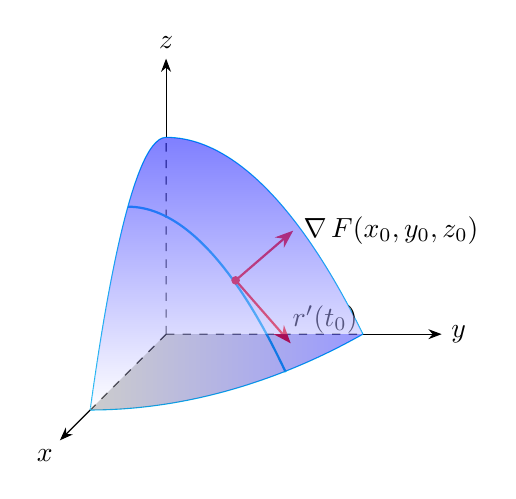
\begin{tikzpicture}[=>stealth]
\draw[-Stealth](2.5,0,0)--(3.5,0,0)node[right]{$y$};
\draw[-Stealth](0,2.5,0)--(0,3.5,0)node[above]{$z$};
\draw[-Stealth](0,0,2.5)--(0,0,3.5);
\draw(0,0,4)node[]{$x$};
\draw[dashed](0,0,0)--(2.5,0,0)
(0,0,0)--(0,2.5,0)
(0,0,0)--(0,0,2.5);
\draw[cyan](2.5,0,0)parabola[bend at end](0,0,2.5)
(0,0,2.5)parabola[bend at  end](0,2.5,0)
(2.5,0,0)parabola[bend at end](0,2.5,0);
\draw[thick,cyan](2,0,1.25)parabola[bend at end](0,2.1,1.25);
\draw(2,1.8,2.9)node[shape=circle,fill=red,draw=red,scale=0.01cm]{};
\draw[-Stealth,thick,red](2,1.8,2.9)--(2,1.7,1)node[right,black]{$\nabla\, F(x_0,y_0,z_0)$};
\draw[-Stealth,thick,red](2,1.8,2.9)--(2.7,1,2.9);
\draw(2.6,1.3,2.9)node[right]{$r'(t_0)$};
\shade[top color=blue,opacity=0.5](0,2.5,0)parabola(2.5,0,0)--(2.5,0,0)--(0,0,0)--(0,2.5,0)--cycle
(0,2.5,0)parabola(0,0,2.5)--(0,0,2.5)--(0,0,0)--(0,2.5,0)--cycle;
\shade[right color=blue,opacity=0.4](2.5,0,0)parabola[bend at end](0,0,2.5)--(0,0,2.5)--(0,0,0)--(2.5,0,0)--cycle;
%\shade[top color=blue,opacity=0.4](0,2.5,0)parabola(2.5,0,0)--(2.5,0,0)parabola[bend at end](0,0,2.5)--(0,0,2.5)parabola[bend at end](0,2.5,0)--cycle;
\end{tikzpicture}
\end{figure}

If $\nabla F(x_0, y_0, z_0) \neq \mathbf 0$, the \emph{tangent plane} to the
level surface $F(x,y,z) = k$ at $P$ is defined as the plane through $P$ with
normal vector $\nabla F(x_0, y_0, z_0)$:
\[F_x(x_0, y_0, z_0)(x -x_0) + F_y(x_0, y_0, z_0)(y -y_0) + F_z(x_0, y_0,
z_0)(z -z_0) = 0 .\]
The \emph{normal line} to $S$ at $P$ is the line through $P$ in the direction of
$\nabla F(x_0,y_0,z_0)$, with symmetric equations
\[ \frac{x - x_0}{F_x (x_0, y_0, z_0)}  = \frac{y - y_0}{F_y (x_0, y_0, z_0)} =
\frac{z - z_0}{F_z (x_0, y_0, z_0)} ,\]
provided the three partial derivatives are non-zero. A graph $z = f(x,y)$ is the
level surface $F = f(x,y) - z = 0$, and with $\nabla F = \langle f_x, f_y,
-1\rangle$ this recovers the tangent plane of the subsection on tangent planes.

\begin{exa}
\label{ex:tangentellipsoid}
Find the equation of the tangent plane and normal line at the point $(-2,1,-3)$
to the ellipsoid
\[\frac{x^2}{4} + y^2 + \frac{z^2}{9} =3 .\]
\end{exa}

\begin{solution}
Let $F = \frac{x^2}{4} + y^2 + \frac{z^2}{9}$. Then
\[\nabla F = \left\langle \frac{x}{2}, 2y, \frac{2z}{9}\right\rangle,\qquad
\nabla F(-2,1,-3) = \left\langle -1, 2, -\frac{2}{3}\right\rangle .\]
The tangent plane is
\[-(x+2) + 2(y-1) -\frac{2}{3}(z + 3) = 0,\qquad\text{that is}\qquad 3x - 6y +
2z + 18 = 0 ,\]
and the normal line has symmetric equations
\[\frac{x + 2}{-1} = \frac{y - 1}{2} = \frac{z + 3}{-2/3} .\]
\end{solution}

\begin{exa}
\label{ex:orthogonalsurfaces}
Show that every sphere centred at the origin meets the cone $z^2 = x^2 + y^2$ at
right angles.
\end{exa}

\begin{solution}
Two surfaces meet at right angles at a common point when their normals there are
perpendicular. The sphere $x^2 + y^2 + z^2 = a^2$ has normal $\langle 2x, 2y,
2z\rangle$, and the cone $x^2 + y^2 - z^2 = 0$ has normal $\langle 2x, 2y,
-2z\rangle$. Their dot product is
\[4(x^2 + y^2 - z^2) = 0\]
at every point of the cone. So at every point where the sphere and the cone
meet (apart from the vertex, where the cone has no tangent plane), the surfaces
are perpendicular. In spherical coordinates this is clear: the sphere is
$\rho = a$ and the cone is $\phi = \frac{\pi}{4}$, coordinate surfaces of an
orthogonal system.
\end{solution}

\begin{exa}
\label{ex:tangentparallel}
Find the points on the hyperboloid $x^2 - 2y^2 - 4z^2 = 16$ at which the tangent
plane is parallel to the plane $4x - 2y + 4z = 5$.
\end{exa}

\begin{solution}
The normal $\nabla F = \langle 2x, -4y, -8z\rangle$ must be a multiple of
$\langle 4,-2,4\rangle$: $2x = 4t$, $-4y = -2t$, $-8z = 4t$, so $x = 2t$,
$y = \frac{t}{2}$, $z = -\frac{t}{2}$. Substituting into the equation,
$4t^2 - \frac{t^2}{2} - t^2 = 16$, so $\frac{5t^2}{2} = 16$ and
$t = \pm\frac{4\sqrt{10}}{5}$. The points are
$\pm\left(\frac{8\sqrt{10}}{5}, \frac{2\sqrt{10}}{5},
-\frac{2\sqrt{10}}{5}\right)$.
\end{solution}


\subsection{Practice Problems}

Each problem is worked in full.

\begin{problem}
\begin{enumerate}
\item[(a)] Find the traces of $f(x,y) = x^2+y^2$ in the planes $x=k$, $y=k$,
$z=k$, and use them to sketch the graph.
\item[(b)] Sketch $g(x,y) = -x^2-y^2$. How is it related to $f$?
\item[(c)] Sketch $h(x,y) = 3-x^2-y^2$. How is it related to $g$?
\end{enumerate}
\end{problem}
\begin{solution}
\subhead{(a)}
In $x=k$: $z = k^2+y^2$, an upward parabola in the $yz-$plane, raised by $k^2$.
In $y=k$: $z = x^2+k^2$, likewise. In $z=k$: $x^2+y^2 = k$, a circle of radius
$\sqrt k$ for $k\geq 0$, a single point for $k=0$, and nothing for $k<0$.

Stacking circles of radius $\sqrt k$ at height $k$, with parabolic vertical
sections, gives a circular paraboloid opening upward with vertex at the origin.

\subhead{(b)}
$g = -f$, so the graph is the reflection of $f$ in the plane $z=0$: the same
paraboloid opening \emph{downward}.

\subhead{(c)}
$h = g+3$, so the graph is that of $g$ translated three units upward: a
downward paraboloid with vertex $(0,0,3)$.
\end{solution}

\begin{problem}
Sketch and identify the surfaces
\[(a)\ 16x^2-9y^2+36z^2 = 144\qquad (b)\ y^2+4z^2 = x .\]
\end{problem}
\begin{solution}
\subhead{(a)}
divide by $144$:
\[\frac{x^2}{9} - \frac{y^2}{16} + \frac{z^2}{4} = 1 .\]
Two positive terms and one negative, with the right-hand side positive: a
\emph{hyperboloid of one sheet}, with axis along $y$, the variable carrying the
minus sign. The trace in $y=k$ is the ellipse
$\dfrac{x^2}{9}+\dfrac{z^2}{4} = 1+\dfrac{k^2}{16}$, which exists for every $k$
and grows with $\left|k\right|$ --- so the surface is connected, as one sheet
requires.

\subhead{(b)}
Only one variable appears to the first power, so this is a paraboloid opening
along $x$. The trace in $x=k$ is the ellipse $y^2+4z^2 = k$, present only for
$k\geq 0$: an \emph{elliptic paraboloid} with vertex at the origin, opening in
the positive $x$ direction.
\end{solution}

\begin{problem}
\begin{enumerate}
\item[(a)] Find and identify the traces of $x^2+y^2-z^2 = 1$.
\item[(b)] How does the graph change for $x^2-y^2+z^2 = 1$?
\item[(c)] What about $x^2+y^2+2y-z^2 = 0$?
\end{enumerate}
\end{problem}
\begin{solution}
\subhead{(a)}
In $z=k$: $x^2+y^2 = 1+k^2$, circles that widen as $\left|k\right|$ grows.
In $x=k$: $y^2-z^2 = 1-k^2$, hyperbolas, degenerating to the pair of lines
$y=\pm z$ when $k=\pm 1$. In $y=k$ likewise. The surface is a
\emph{hyperboloid of one sheet} about the $z-$axis.

\subhead{(b)}
The same surface with the roles of $y$ and $z$ exchanged: a hyperboloid of one
sheet about the $y-$axis. The shape is unchanged; only the axis moves, since it
is always the variable carrying the minus sign.

\subhead{(c)}
Completing the square in $y$,
\[x^2+(y+1)^2-z^2 = 1 ,\]
the same hyperboloid of one sheet, translated one unit in the negative $y$
direction. Its axis is the line $x=0$, $y=-1$.
\end{solution}

\begin{problem}
Sketch the region bounded by $z = x^2+y^2$ and $x^2+y^2 = 1$ for
$1\leq z\leq 2$.
\end{problem}
\begin{solution}
The paraboloid $z = x^2+y^2$ meets the cylinder $x^2+y^2 = 1$ where $z=1$, in
the circle of radius $1$ at that height.

The region is bounded below by the paraboloid, on the outside by the cylinder,
and above by the plane $z=2$. In cylindrical coordinates it is
\[\{(r,\theta,z): 0\leq r\leq 1,\ 0\leq\theta\leq 2\pi,\ r^2\leq z\leq 2\}
\quad\text{together with}\quad 1\leq z\leq 2 ,\]
that is, the solid between the bowl of the paraboloid and the plane $z=2$,
contained within the cylinder --- a cylindrical tub with a paraboloidal floor.
\end{solution}

\begin{problem}
Sketch the region bounded by the paraboloids $z = x^2+y^2$ and
$z = 2-x^2-y^2$.
\end{problem}
\begin{solution}
The two meet where $x^2+y^2 = 2-x^2-y^2$, that is $x^2+y^2 = 1$, at height
$z = 1$.

The first opens upward from the origin, the second downward from $(0,0,2)$. The
region between them is a lens-shaped solid, circular in horizontal section, with
its widest circle of radius $1$ at height $1$, closing to points at $(0,0,0)$
below and $(0,0,2)$ above.
\end{solution}

\begin{problem}
Identify the surface $x^2-y^2+z^2-4x-2y-2z+4 = 0$ and give its centre.
\end{problem}
\begin{solution}
Complete the square in each variable, watching the sign on $y$:
\[(x^2-4x) - (y^2+2y) + (z^2-2z) + 4 = 0\]
\[(x-2)^2-4 - [(y+1)^2-1] + (z-1)^2-1 + 4 = 0\]
\[(x-2)^2 - (y+1)^2 + (z-1)^2 = 0 .\]
The right-hand side is \emph{zero}, not a positive constant, so this is not a
hyperboloid but a \emph{cone}, with axis parallel to the $y-$axis and vertex ---
the point usually called the centre --- at $(2,-1,1)$.

The degenerate case is easy to miss: the same equation with $1$ on the right
would be a hyperboloid of one sheet, and with $-1$ a hyperboloid of two sheets.
The cone is the surface separating those two families.
\end{solution}

\begin{problem}
Find an equation of the surface obtained by revolving each curve about the
indicated axis.
\[(a)\ x^2+4z^2 = 16;\ z\text{-axis}\quad 
(b)\ z = 4-y^2;\ z\text{-axis}\quad 
(c)\ z^2-x^2 = 1;\ x\text{-axis}\quad 
(d)\ z = e^{-y^2};\ y\text{-axis}\]
\end{problem}
\begin{solution}
Revolving about an axis replaces the distance from that axis by
the square root of the sum of the squares of the two coordinates perpendicular to it.

\subhead{(a)} About $z$, the coordinate $x$ is replaced by
$\sqrt{x^2+y^2}$:
\[x^2+y^2+4z^2 = 16 ,\]
an ellipsoid of revolution (oblate, since the $z$ semi-axis is $2$ against $4$).

\subhead{(b)} About $z$, $y$ is replaced by $\sqrt{x^2+y^2}$:
\[z = 4-(x^2+y^2),\]
a downward circular paraboloid with vertex $(0,0,4)$.

\subhead{(c)} About $x$, $z$ is replaced by $\sqrt{y^2+z^2}$:
\[y^2+z^2-x^2 = 1 ,\]
a hyperboloid of one sheet about the $x-$axis.

\subhead{(d)} About $y$, $z$ is replaced by $\sqrt{x^2+z^2}$:
\[\sqrt{x^2+z^2} = e^{-y^2},\qquad\text{that is}\qquad
x^2+z^2 = e^{-2y^2},\]
a bell-shaped surface of revolution, widest at $y=0$ where the radius is $1$.
\end{solution}

\begin{problem}
\begin{enumerate}
\item[(a)] A point has spherical coordinates
$\left(\sqrt8, \dfrac{\pi}{3}, \dfrac{\pi}{4}\right)$. Express it in rectangular
and cylindrical coordinates.
\item[(b)] Express the circle $x^2+y^2+z^2 = 32$, $z = 4$ in spherical and in
cylindrical coordinates.
\end{enumerate}
\end{problem}
\begin{solution}
\subhead{(a)}
With $\rho = \sqrt8 = 2\sqrt2$, $\phi = \dfrac{\pi}{3}$,
$\theta = \dfrac{\pi}{4}$,
\[x = \rho\sin\phi\cos\theta = 2\sqrt2\cdot\frac{\sqrt3}{2}\cdot\frac{1}{\sqrt2}
= \sqrt3 ,\]
and by the same calculation with $\sin\theta$, $y = \sqrt3$, while
\[z = \rho\cos\phi = 2\sqrt2\cdot\frac12 = \sqrt2 .\]
So the rectangular coordinates are $(\sqrt3, \sqrt3, \sqrt2)$.

In cylindrical coordinates $r = \sqrt{x^2+y^2} = \sqrt6$, the angle is
unchanged at $\theta = \dfrac{\pi}{4}$, and $z = \sqrt2$, giving
$\left(\sqrt6, \dfrac{\pi}{4}, \sqrt2\right)$.

\subhead{(b)}
The sphere gives $\rho = \sqrt{32} = 4\sqrt2$. The plane $z=4$ gives
$\rho\cos\phi = 4$, so
\[\cos\phi = \frac{4}{4\sqrt2} = \frac{1}{\sqrt2}\implies \phi = \frac{\pi}{4}.\]
In spherical coordinates the circle is therefore
$\rho = 4\sqrt2$, $\phi = \dfrac{\pi}{4}$, with $\theta$ free.

In cylindrical coordinates, $r^2 = 32-z^2 = 32-16 = 16$, so it is
$r = 4$, $z = 4$, again with $\theta$ free.
\end{solution}

\begin{problem}
A surface is given in spherical coordinates by $\rho\sin^2\phi = \cos\phi$.
Sketch it and give its rectangular equation.
\end{problem}
\begin{solution}
Multiply both sides by $\rho$, which introduces no new points other than the
origin:
\[\rho^2\sin^2\phi = \rho\cos\phi .\]
Now $\rho\sin\phi$ is the distance from the $z-$axis, so
$\rho^2\sin^2\phi = x^2+y^2$, and $\rho\cos\phi = z$. Hence
\[x^2+y^2 = z ,\]
a circular paraboloid opening upward with vertex at the origin.

Recognising $\rho\sin\phi$ and $\rho\cos\phi$ as the cylindrical radius and the
height is what makes the conversion immediate.
\end{solution}

\begin{problem}
A solid $E$ lies within $x^2+y^2+z^2 = 7$, above the $xy-$plane and below the
cone $z = \sqrt{x^2+y^2}$. Sketch it and describe it in spherical coordinates.
\end{problem}
\begin{solution}
The cone $z = \sqrt{x^2+y^2}$ makes an angle of $\dfrac{\pi}{4}$ with the
positive $z-$axis, since there $\rho\cos\phi = \rho\sin\phi$.

"Below the cone" and "above the $xy-$plane" therefore means $\phi$ runs from
$\dfrac{\pi}{4}$ to $\dfrac{\pi}{2}$, and the sphere bounds $\rho$. So
\[E = \left\{(\rho,\phi,\theta): 0\leq\rho\leq\sqrt7,\
\frac{\pi}{4}\leq\phi\leq\frac{\pi}{2},\ 0\leq\theta\leq 2\pi\right\},\]
the part of the ball lying outside the cone and above the equatorial plane ---
a shape like a thick lens with a conical bite taken out of its upper face.
\end{solution}

\begin{problem}
Find the tangent plane to $z^2-2x^2-2y^2 = 12$ at $(1,-1,4)$.
\end{problem}
\begin{solution}
The point satisfies the equation: $16-2-2 = 12$. With
$F = z^2-2x^2-2y^2-12$,
\[\nabla F = \langle -4x, -4y, 2z\rangle
\ \longrightarrow\ \langle -4, 4, 8\rangle .\]
The tangent plane through $(1,-1,4)$ with this normal is
\[-4(x-1) + 4(y+1) + 8(z-4) = 0 ,\]
which simplifies, on dividing by $4$, to
\[-x + y + 2z = 6 .\]
\end{solution}

\begin{problem}
Find the tangent plane to $2xz^2-3xy-4x = 7$ at $(1,-1,2)$.
\end{problem}
\begin{solution}
The point satisfies the equation: $2(1)(4) - 3(1)(-1) - 4 = 8+3-4 = 7$. With
$G = 2xz^2-3xy-4x-7$,
\[\nabla G = \langle 2z^2-3y-4,\ -3x,\ 4xz\rangle
\ \longrightarrow\ \langle 8+3-4,\ -3,\ 8\rangle = \langle 7,-3,8\rangle .\]
Hence the tangent plane is
\[7(x-1) - 3(y+1) + 8(z-2) = 0 ,\]
that is $7x-3y+8z = 26$.
\end{solution}

\begin{problem}
Let $9x^2-36x+4y^2+8y+18z^2+108z-158 = 0$.
\begin{enumerate}
\item[(a)] Identify the surface and give its centre.
\item[(b)] Find the tangent plane at
$\left(3, 2, 3+\dfrac{1}{\sqrt2}\right)$.
\end{enumerate}
\end{problem}
\begin{solution}
\subhead{(a)}
Completing the square in each variable,
\[9(x-2)^2 - 36 + 4(y+1)^2 - 4 + 18(z+3)^2 - 162 - 158 = 0 ,\]
\[9(x-2)^2 + 4(y+1)^2 + 18(z+3)^2 = 360 ,\]
and dividing by $360$,
\[\frac{(x-2)^2}{40} + \frac{(y+1)^2}{90} + \frac{(z+3)^2}{20} = 1 .\]
All three terms are positive, so this is an \emph{ellipsoid}, with centre
$(2,-1,-3)$ and semi-axes $\sqrt{40}$, $\sqrt{90}$, $\sqrt{20}$.

\subhead{(b)}
The point given does not lie on the surface. Substituting
$x=3$, $y=2$, $z = 3+\dfrac{1}{\sqrt2}$ into the left-hand side gives
\[9(1) + 4(9) + 18(6+\tfrac{1}{\sqrt2})^2 \approx 854.7 ,\]
against the required $360$; equivalently the original expression evaluates to
$(18+3\sqrt2)^2\approx 494.7$ rather than $0$. Since the centre has
$z=-3$ and the $z$ semi-axis is only $\sqrt{20}\approx 4.47$, no point of the
surface has $z$ anywhere near $3.7$.

The tangent plane is therefore computed at the point of the surface with the
same $x$ and $y$. Putting $x=3$, $y=2$ gives
$18(z+3)^2 = 360-45 = 315$, so $z = -3+\dfrac{\sqrt{70}}{2}\approx 1.183$.
There
\[\nabla F = \langle 18x-36,\ 8y+8,\ 36z+108\rangle
= \langle 18,\ 24,\ 18\sqrt{70}\rangle ,\]
and dividing by $6$, a normal is
$\langle 3, 4, 3\sqrt{70}\rangle$. The tangent plane is
\[3(x-3) + 4(y-2) + 3\sqrt{70}\left(z+3-\frac{\sqrt{70}}{2}\right) = 0 ,\]
that is
\[3x + 4y + 3\sqrt{70}\,z = 122 - 9\sqrt{70} .\]
\end{solution}

\begin{problem}
Find symmetric equations for the normal line to $xyz = 6$ at $(2,3,1)$.
\end{problem}
\begin{solution}
The point satisfies the equation, since $2\cdot 3\cdot 1 = 6$. With
$F = xyz-6$,
\[\nabla F = \langle yz, xz, xy\rangle
\ \longrightarrow\ \langle 3, 2, 6\rangle .\]
The normal line runs through $(2,3,1)$ in that direction, so
\[\frac{x-2}{3} = \frac{y-3}{2} = \frac{z-1}{6}.\]
\end{solution}

\begin{problem}
Find a unit normal to $x^2y+2xz = 4$ at $(2,-2,3)$.
\end{problem}
\begin{solution}
The point satisfies the equation: $4(-2)+2(2)(3) = -8+12 = 4$. With
$K = x^2y+2xz-4$,
\[\nabla K = \langle 2xy+2z,\ x^2,\ 2x\rangle
\ \longrightarrow\ \langle -8+6,\ 4,\ 4\rangle = \langle -2, 4, 4\rangle .\]
Its length is $\sqrt{4+16+16} = 6$, so the unit normals are
\[\pm\frac{1}{6}\langle -2,4,4\rangle
= \pm\left\langle -\frac13, \frac23, \frac23\right\rangle .\]
\end{solution}

\begin{problem}
A heat-seeking particle sits at $(2,-3)$ on a plate whose temperature is
$T(x,y) = 20-4x^2-y^2$. In which direction should it move to warm fastest, and
how fast does the temperature rise in that direction?
\end{problem}
\begin{solution}
\[\nabla T = \langle -8x, -2y\rangle
\ \longrightarrow\ \nabla T(2,-3) = \langle -16, 6\rangle .\]
The particle should move along the gradient, in the direction of the unit vector
\[\frac{1}{\sqrt{256+36}}\langle -16, 6\rangle
= \frac{1}{2\sqrt{73}}\langle -16, 6\rangle
= \frac{1}{\sqrt{73}}\langle -8, 3\rangle ,\]
and the rate of increase in that direction is
$\left|\nabla T\right| = 2\sqrt{73}\approx 17.1$ degrees per unit length.

The direction points back towards the origin, where the plate is hottest, which
is the check worth making.
\end{solution}

\begin{problem}
Find the angle between the surfaces $x^2+y^2+z^2 = 9$ and $z = x^2+y^2-3$ at
$(2,-1,2)$.
\end{problem}
\begin{solution}
Both pass through the point: $4+1+4 = 9$, and $4+1-3 = 2$.

The angle between two surfaces at a common point is the angle between their
normals there. For the sphere, $\nabla(x^2+y^2+z^2) = \langle 2x,2y,2z\rangle$
gives $\mathbf{n}_1 = \langle 4,-2,4\rangle$. For the paraboloid, written as
$x^2+y^2-z-3 = 0$, the gradient is $\langle 2x,2y,-1\rangle$, giving
$\mathbf{n}_2 = \langle 4,-2,-1\rangle$. Then
\[\cos\theta
= \frac{16+4-4}{\sqrt{36}\sqrt{21}} = \frac{16}{6\sqrt{21}}
= \frac{8\sqrt{21}}{63}\approx 0.582 ,\]
so $\theta\approx 54.4^{\circ}$.
\end{solution}


\section{Multiple Integration}

The definite integral of one variable adds up a quantity along an interval. The
multiple integral does the same over a region of the plane or of space, and the
construction is the same in every case: cut the region into small pieces,
multiply the value of the function on each piece by its area or volume, add, and
pass to the limit.

The practical content of the section is that such an integral can be evaluated
as a succession of ordinary single integrals. That is Fubini's theorem, and it
is what makes the subject computable rather than merely definable. The work then
becomes a matter of describing the region correctly and choosing the order of
integration well, which is why so much attention goes to regions of Type I and
Type II and to reversing the order.

Polar, cylindrical and spherical coordinates follow, each earning its place by
turning a region with an awkward boundary into a rectangle. The change of
variables formula unifies them: the Jacobian of the previous section reappears
as the factor by which the change of coordinates stretches area or volume, and
it is exactly what must be inserted to keep the answer right.

The section closes with the applications the machinery was built for --- volume,
mass, centre of mass, moments of inertia and surface area.

Recall the single-variable construction. For $f\geq 0$ on $[a,b]$, divide the
interval into $n$ subintervals of width $\Delta x$, choose a sample point
$x_i^*$ in each, and approximate the area under the curve by rectangles.

\begin{figure}[H]
\centering
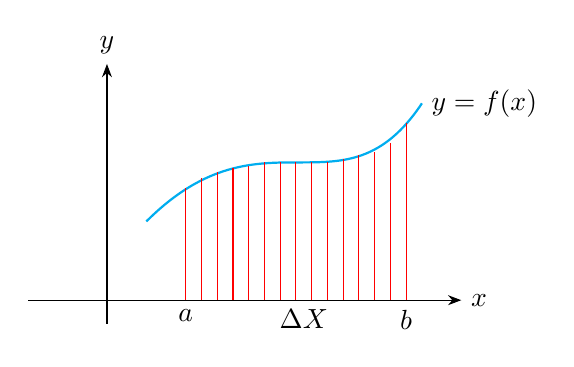
\begin{tikzpicture}[=>stealth]
\draw[-Stealth](-1,0)--(4.5,0)node[right]{$x$};
\draw[-Stealth](0,-0.3)--(0,3)node[above]{$y$};
\draw[thick,cyan](0.5,1)..controls(2,2.5)and (3,1)..(4,2.5);
\draw[red](1,0)--(1,1.43);
\draw[red](3.8,0)--(3.8,2.25);
\draw[red](2.6,0)--(2.6,1.75)
(2.4,0)--(2.4,1.75)
(2.2,0)--(2.2,1.75)
(2,0)--(2,1.75)
(1.8,0)--(1.8,1.7)
(1.6,0)--(1.6,1.68)
(1.4,0)--(1.4,1.63)
(1.2,0)--(1.2,1.55)
(2.8,0)--(2.8,1.75)
(3,0)--(3,1.79)
(3.2,0)--(3.2,1.84)
(3.4,0)--(3.4,1.88)
(3.6,0)--(3.6,2);
\draw(1,0)node[below]{$a$}
(3.8,0)node[below]{$b$}
(4,2.5)node[right]{$y = f(x)$}
(2.5,0)node[below]{$\Delta X$};
\end{tikzpicture}
\end{figure}

The area under the curve is the limit of the Riemann sums,
\[\int^b_a f(x)\,dx = \lim_{n\to\infty}\sum^{n}_{i=1} f(x_i^*)\, \Delta x ,\]
each term being the area of one approximating rectangle.

{\color[wave]{485}\subsection{Volumes and Double Integration}}

In the same way, consider a function $f$ of two variables defined on a closed
rectangle
\[R = [a,b]\times [c,d] = \{(x,y)\in \mathbb{R}^2 \mid a\leq x\leq b,\ c \leq y
\leq d\},\]
and suppose first that $f(x,y)\geq 0$.

\begin{figure}[H]
\centering
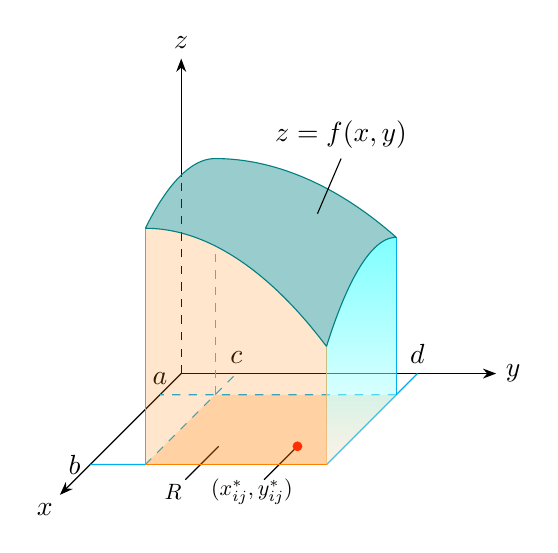
\begin{tikzpicture}[=>stealth]
\draw[-Stealth](0,0,0)--(4,0)node[right]{$y$};
\draw[-Stealth](0,2.5,0)--(0,4,0)node[above]{$z$};
\draw[-Stealth](0,0,0)--(0,0,4);
\draw(0,0,4.5)node[]{$x$};
\draw[dashed](0,0,0)--(0,2.5,0);
%\draw(0.7,0,0.7)--(0.7,0,3)--(3,0,3)--(3,0,0.7)--cycle;
\draw[cyan](0.7,0,3)--(0,0,3)node[left,black]{$b$}
(3,0,3)--(3,0,0)node[above,black]{$d$};
\draw[cyan,dashed](3,0,0.7)--(0,0,0.7)node[above,black]{$a$}
(0.7,0,3)--(0.7,0,0)node[above,black]{$c$};
\draw(2.4,0,2.4)node[shape=circle,fill=red,draw=red,thick,scale=0.01cm]{}
(2.4,0,2.4)--(2.4,0,3.5)
(1.4,0,2.4)--(1.4,0,3.5)
(1.4,0,3.9)node[scale=0.8]{$R$}
(2.4,0,3.9)node[scale=0.8]{$(x_{ij}^*,y_{ij}^*$)};
\draw[orange](0.7,0,3)--(0.7,3,3)
(0.7,0,3)--(3,0,3)
(3,0,3)--(3,1.5,3);
\draw[orange,dashed](0.7,0,0.7)--(0.7,1.8,0.7);
\path[fill=orange,opacity=0.2](0.7,0,0.7)--(0.7,0,3)--(3,0,3)--(3,0,0.7)--cycle;
\path[fill=orange,opacity=0.2](0.7,0,3)--(3,0,3)--(3,1.5,3)parabola[bend at end](0.7,3,3)--(0.7,3,3)--cycle;
\shade[top color=cyan,opacity=0.5](3,0,0.7)--(3,2,0.7)parabola(3,1.5,3)--(3,0,3)--cycle;
\draw[cyan](3,0,0.7)--(3,2,0.7);
\draw[color=teal](3,1.5,3)parabola[bend at end](0.7,3,3)
(3,2,0.7)parabola(3,1.5,3)
(0.7,3,0.7)parabola(3,2,0.7)
(0.7,3,0.7)parabola(0.7,3,3);
\path[fill=teal,opacity=0.4](0.7,3,3)parabola(3,1.5,3)--(3,1.5,3)parabola[bend at end](3,2,0.7)--(3,2,0.7)parabola[bend at end](0.7,3,0.7)--(0.7,3,0.7)parabola(0.7,3,3);
\draw(2,2.3,0.7)--(2.3,3,0.7)node[above]{$z=f(x,y)$};
\end{tikzpicture}
\end{figure}

Let $S$ be the solid that lies above $R$ and under the graph of $f$,
\[S = \{(x,y,z)\in \mathbb{R}^3 \mid (x,y)\in R,\ 0\leq z \leq f(x,y)\} .\]
The aim is to find the volume of $S$. Divide $[a,b]$ into $m$ subintervals of
width $\Delta x$ and $[c,d]$ into $n$ of width $\Delta y$. The lines through
the division points cut $R$ into $mn$ subrectangles $R_{ij}$, each of area
$\Delta A = \Delta x\,\Delta y$, and in each we choose a sample point
$(x^*_{ij},y^*_{ij})$.

\begin{figure}[H]
\centering
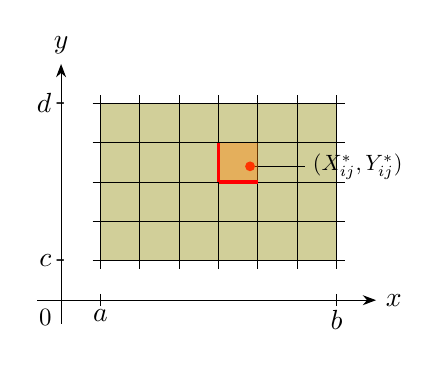
\begin{tikzpicture}[=>stealth]
\draw[-Stealth](-0.3,0)--(4,0)node[right]{$x$};
\draw[-Stealth](0,-0.3)--(0,3)node[above]{$y$};
\draw(0.5,0.5)--(3.5,0.5)--(3.5,2.5)--(0.5,2.5)--cycle;
\path[fill=olive,opacity=0.4](0.5,0.5)--(3.5,0.5)--(3.5,2.5)--(0.5,2.5)--cycle;
\draw[step=0.5cm](0.4,0.4)grid(3.6,2.6);
\draw(0.5,0.08)--(0.5,-0.08)
(3.5,0.08)--(3.5,-0.08)
(0,0.5)node[]{-}
(0,2.5)node[]{-}
(0.5,0)node[below]{$a$}
(3.5,0)node[below]{$b$}
(0,0.5)node[left]{$c$}
(0,2.5)node[left]{$d$}
(2.4,1.7)node[shape=circle,fill=red,draw=red,thick,scale=0.01cm]{}
(2.4,1.7)--(3.1,1.7)node[right,scale=0.8]{$(X_{ij}^*,Y_{ij}^*)$}
(-0.2,0)node[below,scale=0.9]{0};
\path[fill=orange,opacity=0.4](2,1.5)--(2.5,1.5)--(2.5,2)--(2,2)--cycle;
\draw[very thick,red](2,1.5)--(2,2);
\draw[very thick,red](2,1.5)--(2.5,1.5);
\end{tikzpicture}
\end{figure}

The part of $S$ above $R_{ij}$ is approximated by a thin rectangular box with
base $R_{ij}$ and height $f(x^*_{ij},y^*_{ij})$, whose volume is
$f(x^*_{ij},y^*_{ij})\,\Delta A$. Adding,
\[V \approx \sum^m_{i=1}\sum^n_{j=1}f(x^*_{ij},y^*_{ij})\,\Delta A ,\]
a \emph{double Riemann sum}, and the approximation improves as the rectangles
shrink.

\begin{defn}
\label{defn:doubleintegral}
The \emph{double integral} of $f$ over the rectangle $R$ is
\[\iint\limits_R f(x,y)\,dA = \lim_{m,n\to \infty}\sum^m_{i=1}\sum^n_{j=1}
f(x^*_{ij},y^*_{ij})\,\Delta A\]
if the limit exists, with the same value for every choice of sample points. If
$f(x,y)\geq 0$, the volume of the solid that lies above $R$ and below the
surface $z = f(x,y)$ is
\[V = \iint\limits_R f(x,y)\, dA .\]
\end{defn}

Every continuous function on $R$ is integrable, and so is every bounded function
whose discontinuities lie on finitely many smooth curves. When $f$ takes both
signs, the integral is the volume above the $xy$-plane minus the volume below
it.

\begin{exa}
\label{ex:halfcylinder}
If $R = \{ (x,y) \mid -1\leq x \leq 1,\ -2\leq y\leq 2\}$, evaluate
\[\iint\limits_R \sqrt{1 - x^2}\, dA .\]
\end{exa}

\begin{solution}
The integrand is non-negative, so the integral is a volume. The surface
$z = \sqrt{1 - x^2}$ satisfies $x^2 + z^2 = 1$ with $z\geq 0$, and $y$ does not
appear: it is the upper half of the circular cylinder of radius $1$ about the
$y$-axis.

\begin{figure}[H]
\centering
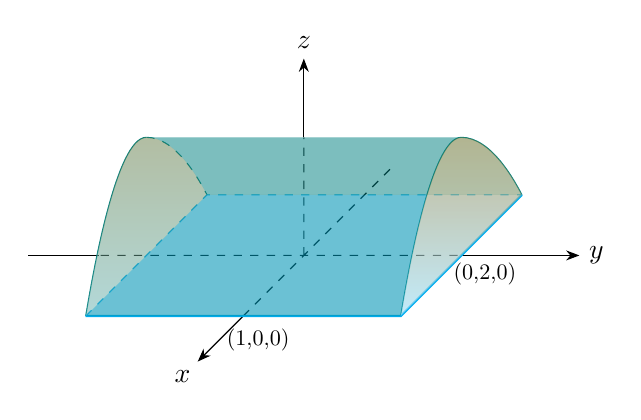
\begin{tikzpicture}[=>stealth]
\draw[-Stealth](2,0,0)--(3.5,0,0)node[right]{$y$};
\draw[-Stealth](0,1.5,0)--(0,2.5,0)node[above]{$z$};
\draw[-Stealth](0,0,2)--(0,0,3.5);
\draw[dashed](-2.58,0,0)--(2,0,0)
(0,0,2)--(0,0,-3)
(0,0,0)--(0,1.5,0);
\draw(0,0,4)node[]{$x$}
(-2.6,0,0)--(-3.5,0,0);
\draw[teal](2,0,2)parabola[bend at end](2,1.5,0)
(2,1.5,0)parabola(2,0,-2)
(-2,1.5,0)parabola(-2,0,2);
\draw[teal,dashed](-2,1.5,0)parabola(-2,0,-2);
\draw[cyan,dashed](-2,0,2)--(-2,0,-2)--(2,0,-2);
\draw[thick,cyan](2,0,-2)--(2,0,2)--(-2,0,2);
\path[fill=cyan,opacity=0.4](-2,0,2)--(-2,0,-2)--(2,0,-2)--(2,0,2)--cycle;
\shade[top color = orange,opacity=0.4](2,0,2)parabola[bend at end](2,1.5,0)--(2,1.5,0)parabola(2,0,-2)--(2,0,-2)--cycle;
\shade[top color=orange,opacity=0.3](-2,0,2)parabola[bend at end](-2,1.5,0)--(-2,1.5,0)parabola(-2,0,-2)--(-2,0,-2)--cycle;
\path[fill = teal,opacity=0.3](2,0,2)parabola[bend at end](2,1.5,0)--(2,1.5,0)--(-2,1.5,0)parabola(-2,0,2)--(-2,0,2)--cycle;
\path[fill = teal,opacity=0.3](2,1.5,0)parabola(2,0,-2)--(2,0,-2)--(-2,0,-2)--(-2,0,-2)parabola[bend at end](-2,1.5,0)--cycle;
\draw(2.3,0)node[below,scale=0.8]{(0,2,0)}
(0,0,2.8)node[right,scale=0.8]{(1,0,0)};
\end{tikzpicture}
\end{figure}

The solid over $R$ is half of a cylinder of radius $1$ and length $4$, so
\[\iint\limits_R \sqrt{1 - x^2}\, dA = \frac{1}{2}\,\pi\,(1)^2\,(4) = 2\pi .\]
\end{solution}

\begin{exa}
\label{ex:riemannestimate}
Estimate the volume of the solid above $R = [0,2]\times[0,2]$ and below
$z = 16 - x^2 - 2y^2$, using a Riemann sum with four squares and sample points
at their upper right corners.
\end{exa}

\begin{solution}
The squares have $\Delta A = 1$ and upper right corners $(1,1)$, $(1,2)$,
$(2,1)$ and $(2,2)$, where $f$ is $13$, $7$, $10$ and $4$. The estimate is
$(13 + 7 + 10 + 4)\cdot 1 = 34$. Because $f$ decreases in both variables, upper
right corners give the smallest values and the estimate is too low; the exact
value, found in Example~\ref{ex:volumeparaboloid}, is $48$.
\end{solution}

\begin{exa}
\label{ex:midpoint}
Use the midpoint rule with four squares to estimate
$\iint_R (x - 3y^2)\,dA$ over $R = [0,2]\times[1,2]$, divided into four equal
rectangles.
\end{exa}

\begin{solution}
Divide $[0,2]$ into $[0,1]$ and $[1,2]$ and $[1,2]$ into $[1,\frac32]$ and
$[\frac32,2]$, so $\Delta A = \frac12$ and the midpoints are $x = \frac12,
\frac32$ and $y = \frac54, \frac74$. Then
\[\sum f(\bar x_i,\bar y_j)\,\Delta A = \frac12\left[\left(\tfrac12 -
\tfrac{75}{16}\right) + \left(\tfrac12 - \tfrac{147}{16}\right) + \left(\tfrac32 -
\tfrac{75}{16}\right) + \left(\tfrac32 - \tfrac{147}{16}\right)\right] =
-\frac{95}{8} = -11.875 .\]
The exact value, found in Example~\ref{ex:fubinipoly}, is $-12$.
\end{solution}

{\color[wave]{485}\subsection{Iterated Integrals}}

Suppose that $f$ is continuous on the rectangle $R = [a,b]\times [c,d]$. The
notation $\int^d_c f(x,y)\,dy$ means that $x$ is held fixed and $f(x,y)$ is
integrated with respect to $y$ from $c$ to $d$, a process called \emph{partial
integration}. The result is a function of $x$,
\[A(x) = \int^d_c f(x,y)\, dy ,\]
which can then be integrated with respect to $x$ from $a$ to $b$:
\begin{equation}
\int^b_a\int^d_c f(x,y)\,dy\,dx = \int^b_a\left[ \int^d_c f(x,y)\,dy\right] dx .
\label{eq:iterated}
\end{equation}
The integral on the right of \eqref{eq:iterated} is an \emph{iterated
integral}: work from the inside out. Similarly,
\[\int^d_c\int^b_a f(x,y)\,dx\,dy = \int^d_c\left[ \int^b_a f(x,y)\,dx\right] dy
,\]
with $x$ integrated first.

\begin{exa}
\label{ex:iterated}
Evaluate the iterated integrals
\[(a)\quad  \int^3_0\int^2_1 x^2y\,dy\,dx\qquad  (b)\quad  \int^2_1\int^3_0
x^2y\,dx\,dy .\]
\end{exa}

\begin{solution}
\begin{align*}
(a)\qquad \int^3_0\int^2_1 x^2y\,dy\,dx & = \int^3_0\left[ \frac{x^2y^2}{2}
\right]_{y=1}^{y=2} dx = \int^3_0\frac{3}{2}x^2\,dx = \frac{3}{2}\cdot 9 =
\frac{27}{2},\\[1ex]
(b)\qquad \int^2_1\int^3_0 x^2y\,dx\,dy & = \int^2_1\left[\frac{x^3y}{3}
\right]_{x=0}^{x=3} dy = \int^2_1 9y\,dy = 9\cdot\frac32 = \frac{27}{2} .
\end{align*}
The two orders give the same answer, which is no accident.
\end{solution}

\subhead{Fubini's Theorem}

\begin{thm}[Fubini]
\label{thm:fubini}
If $f$ is continuous on the rectangle $R = \{ (x,y) \mid a\leq x \leq b,\
c\leq y\leq d\}$, then
\[\iint\limits_R f(x,y)\, dA = \int^b_a \int^d_c f(x,y)\,dy\, dx = \int^d_c
\int^b_a f(x,y)\,dx\, dy .\]
More generally, the result holds whenever $f$ is bounded on $R$, is
discontinuous only on finitely many smooth curves, and the iterated integrals
exist.
\end{thm}

For $f\geq 0$ the reason is geometric. The integral $A(x) = \int_c^d f(x,y)\,dy$
is the area of the cross-section of the solid $S$ by the plane at $x$, and
integrating the areas of cross-sections gives the volume, as in the method of
slicing for solids of revolution. Slicing by planes $y = \text{constant}$ gives
the same volume.

\begin{exa}
\label{ex:fubinipoly}
Evaluate $\iint_R (x-3y^2)\,dA$, where
$R = \{ (x,y) \mid 0\leq x \leq 2,\ 1 \leq y \leq 2 \}$.
\end{exa}

\begin{solution}
By Fubini's theorem, integrating $y$ first,
\[\iint\limits_R (x-3y^2)\,dA = \int^2_0\left[xy - y^3\right]_{y=1}^{y=2}dx =
\int^2_0 (x - 7)\,dx = 2 - 14 = -12 ,\]
and integrating $x$ first,
\[\int^2_1\left[\frac{x^2}{2} - 3xy^2\right]_{x=0}^{x=2}dy = \int^2_1 (2 -
6y^2)\, dy = 2 - 14 = -12 .\]
The integral is negative because the integrand is negative on most of $R$.
\end{solution}

\begin{exa}
\label{ex:ysinxy}
Evaluate $\iint_R y \sin (xy)\,dA$, where $R = [1,2]\times [0,\pi]$.
\end{exa}

\begin{solution}
\subhead{Integrating in $x$ first, then $y$}
\[\iint\limits_R y \sin (xy) \, dA = \int^{\pi}_0 \Big[-\cos(xy)\Big]_{x=1}^{x=2}
dy = \int^{\pi}_0 (\cos y - \cos 2y)\, dy = \left[\sin y - \frac{\sin
2y}{2}\right]_0^{\pi} = 0 .\]

\subhead{The other order}
Integrating $y\sin(xy)$ with respect to $y$ needs integration by parts:
\[\int^{\pi}_0 y\sin (xy)\,dy = \left[-\frac{y\cos(xy)}{x}\right]_0^{\pi} +
\frac1x\int_0^{\pi}\cos(xy)\,dy = -\frac{\pi \cos \pi x}{x} + \frac{\sin \pi
x}{x^2},\]
and the remaining integral
$\int^2_1 \left( -\frac{\pi \cos \pi x}{x} + \frac{\sin \pi x}{x^2}\right) dx$
is done by noticing that the integrand is the derivative of
$-\frac{\sin \pi x}{x}$. Its value is
$\left[-\frac{\sin \pi x}{x}\right]_1^2 = 0$. The choice of order can turn an
easy integral into a hard one.
\end{solution}

\begin{exa}
\label{ex:volumeparaboloid}
Find the volume of the solid $S$ that is bounded by the elliptic paraboloid
$x^2+ 2y^2 + z = 16$, the planes $x=2$ and $y = 2$, and the three coordinate
planes.

\begin{figure}[H]
\centering
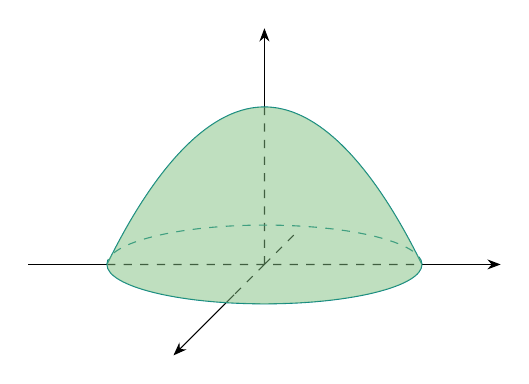
\begin{tikzpicture}[=>stealth]
\draw[dashed](-2,0,0)--(2,0,0)
(0,0,0)--(0,2,0)
(0,0,0)--(0,0,1)
(0,0,0)--(0,0,-1);
\draw[-Stealth](0,2,0)--(0,3,0);
\draw[-Stealth](2,0,0)--(3,0,0);
\draw[-Stealth](0,0,1)--(0,0,3);
\draw(-3,0,0)--(-2,0,0);
\draw[teal](0,2)parabola(2,0)
(0,2)parabola(-2,0);
\draw[teal](-2,0)arc(180:360:2cm and 0.5cm);
\draw[dashed,teal](2,0)arc(0:180:2cm and 0.5cm);
\path[fill=orange!50!cyan,opacity=0.5](0,0)circle(2cm and 0.5cm)--(2,0)parabola[bend at end](0,2)--(0,2)parabola(-2,0);
\end{tikzpicture}
\end{figure}
\end{exa}

\begin{solution}
The solid lies under the surface $z = 16 - x^2 -2y^2$ and above the square
$R = [0,2]\times [0,2]$. By Fubini's theorem,
\begin{align*}
V & = \iint\limits_R ( 16 - x^2 - 2y^2)\, dA = \int^2_0\int^2_0 (16 - x^2 -2y^2
)\,dx\, dy\\
& = \int^2_0\left( 32 - \frac{8}{3} - 4y^2\right)dy = \int^2_0\left(
\frac{88}{3} - 4y^2\right)dy = \frac{176}{3} - \frac{32}{3} = 48 .
\end{align*}
\end{solution}

When the integrand is a product of a function of $x$ alone and a function of $y$
alone, $f(x,y) = g(x)h(y)$, and $R = [a,b]\times[c,d]$, the inner integral
$\int_c^d g(x)h(y)\,dy = g(x)\int_c^d h(y)\,dy$, so the double integral factors:
\[ \iint\limits_R g(x)h(y)\,dA = \int^b_a g(x)\,dx\int^d_c h(y)\,dy .\]

\begin{exa}
\label{ex:separable}
Evaluate $\iint_R \sin x \cos y \, dA$, where
$R = \left[ 0,\frac{\pi}{2}\right] \times \left[ 0,\frac{\pi}{2}\right]$.
\end{exa}

\begin{solution}
\[\iint\limits_R \sin x \cos y \, dA = \int^{\pi/2}_0 \sin x \, dx
\int^{\pi/2}_0\cos y \,dy = 1\cdot 1 = 1 .\]
\end{solution}

\begin{exa}
\label{ex:fubinilog}
Evaluate $\int_0^1\int_1^2 \frac{x}{1 + xy}\,dy\,dx$ and
$\int_0^1\int_0^1 xe^{xy}\,dy\,dx$.
\end{exa}

\begin{solution}
For the first, the inner integral is $\left[\ln(1 + xy)\right]_{y=1}^{y=2} =
\ln(1 + 2x) - \ln(1 + x)$, and
\[\int_0^1\big(\ln(1+2x) - \ln(1+x)\big)\,dx = \left[\tfrac{(1+2x)\ln(1+2x)}{2} -
(1+x)\ln(1+x)\right]_0^1 = \tfrac32\ln 3 - 2\ln 2\approx 0.2616 ,\]
the terms $-x$ from the two antiderivatives cancelling. For the second, the
inner integral is $\left[e^{xy}\right]_{y=0}^{y=1} = e^x - 1$, so the value is
$\int_0^1 (e^x - 1)\,dx = e - 2$. Here integrating $y$ first is essential: in
the other order the inner integral $\int_0^1 xe^{xy}\,dx$ needs integration by
parts and the outer one is harder still.
\end{solution}

{\color[wave]{485}\subsection{Double Integrals Over General Regions}}

Suppose that $D$ is a bounded region, so that it can be enclosed in a rectangle
$R$. Define a new function $F$ with domain $R$ by
\[ F(x,y) =
\begin{cases}
f(x,y), & (x,y)\in D,\\
0, & (x,y)\in R,\ (x,y)\notin D .
\end{cases}
\]
If the double integral of $F$ over $R$ exists, the double integral of $f$ over
$D$ is defined by
\[\iint\limits_D f(x,y)\,dA = \iint\limits_R F(x,y)\,dA .\]
The value does not depend on the rectangle chosen, since $F$ is zero outside
$D$.

A plane region $D$ is of \emph{type I} if it lies between the graphs of two
continuous functions of $x$:
\[ D = \{ (x,y) \mid a \leq x \leq b,\ g_1(x) \leq y\leq g_2(x)\},\]
where $g_1$ and $g_2$ are continuous on $[a,b]$. Vertical lines meet a type I
region in a single segment.

\begin{table}[H]
\centering
\begin{tabular}{ccccccccc}
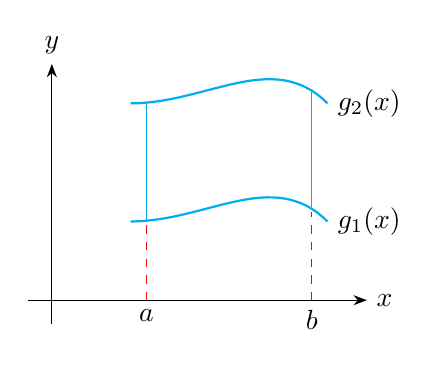
\begin{tikzpicture}[=>stealth]
\draw[-Stealth](-0.3,0)--(4,0)node[right]{$x$};
\draw[-Stealth](0,-0.3)--(0,3)node[above]{$y$};
\draw[cyan,thick,out=0](1,1)to(3.5,1)node[right,black]{$g_1(x)$};
\draw[cyan,thick,out=0](1,2.5)to(3.5,2.5)node[right,black]{$g_2(x)$};
\draw[cyan](1.2,1.02)--(1.2,2.5)
(3.3,1.18)--(3.3,2.65);
\draw[dashed,red](1.2,0)--(1.2,1)
(3.3,0)--(3.3,1.12);
\draw(1.2,0)node[below]{$a$}
(3.3,0)node[below]{$b$};
\end{tikzpicture}
&&&&&&&&
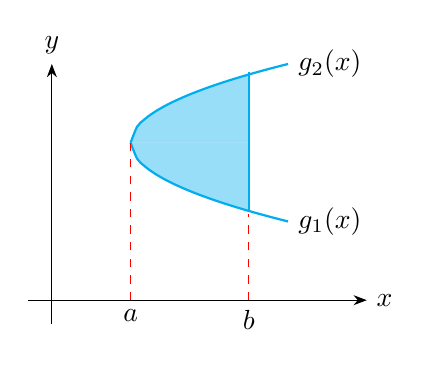
\begin{tikzpicture}[=>stealth]
\draw[-Stealth](-0.3,0)--(4,0)node[right]{$x$};
\draw[-Stealth](0,-0.3)--(0,3)node[above]{$y$};
\draw[smooth,domain=1:3,variable=\x,thick,cyan]plot(\x,{2+1/2*sqrt(2*(\x-1))})node[right,black]{$g_2(x)$};
\draw[smooth,domain=1:3,variable=\x,thick,cyan]plot(\x,{2-1/2*sqrt(2*(\x-1))})node[right,black]{$g_1(x)$};
\draw[dashed,red](1,0)--(1,2)
(2.5,0)--(2.5,1.1);
\draw[thick,cyan](2.5,1.15)--(2.5,2.9);
\draw(1,0)node[below]{$a$}
(2.5,0)node[below]{$b$};
\path[fill=cyan,opacity=0.4,domain=1:2.5,variable=\x]plot(\x,{2+1/2*sqrt(2*(\x-1))})--(2.5,2.9)--(2.5,2.001)--(1,2)--cycle;
\path[fill=cyan,opacity=0.4,domain=1:2.5,variable=\x]plot(\x,{2-1/2*sqrt(2*(\x-1))})--(2.5,1.16)--(2.5,2)--(1,2)--cycle;
\end{tikzpicture}\\
\end{tabular}
\end{table}

\begin{figure}[H]
\centering
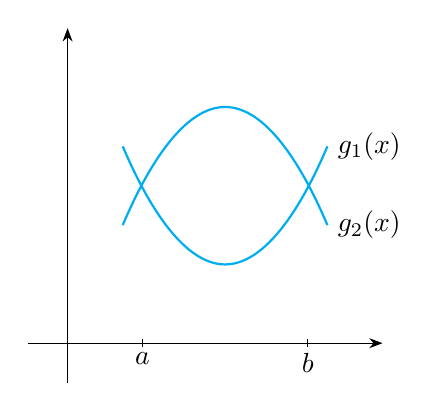
\begin{tikzpicture}[=>stealth]
\draw[-Stealth](-0.5,0)--(4,0);
\draw[-Stealth](0,-0.5)--(0,4);
\draw[thick,cyan](2,1)parabola(3.3,2.5)node[right,black]{$g_1(x)$}
(2,1)parabola(0.7,2.5)
(2,3)parabola(3.3,1.5)node[right,black]{$g_2(x)$}
(2,3)parabola(0.7,1.5);
\draw(0.95,0)node[below]{$a$}
(3.05,0)node[below]{$b$};
\draw(3.05,-0.05)--(3.05,0.05)
(0.95,-0.05)--(0.95,0.05);
\end{tikzpicture}
\end{figure}

To evaluate $\iint_D f(x,y)\,dA$ when $D$ is a type I region, choose a rectangle
$R = [a,b] \times [c,d]$ that contains $D$.

\begin{figure}[H]
\centering
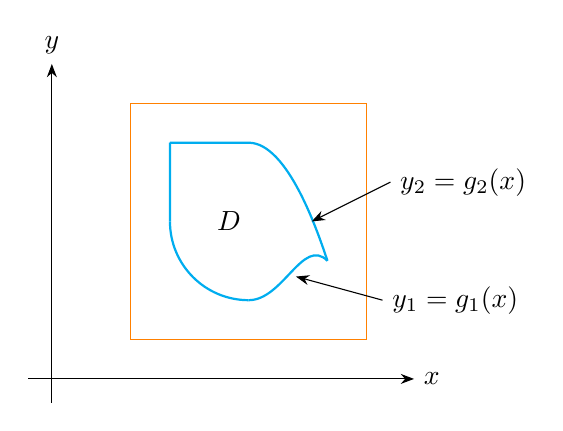
\begin{tikzpicture}[=Stealth]
\draw[-Stealth](-0.3,0)--(4.6,0)node[right]{$x$};
\draw[-Stealth](0,-0.3)--(0,4)node[above]{$y$};
\draw[thick,cyan](1.5,2)arc[start angle=180, end angle=270, radius=1cm];
\draw[thick,cyan](1.5,3)--(2.5,3)
(2.5,3)parabola(3.5,1.5)
(1.5,3)--(1.5,2);
\draw[thick,cyan,out=0](2.5,1)to(3.5,1.5);
\draw(2.25,2)node[]{$D$}
(4.3,2.5)node[right]{$y_2=g_2(x)$}
(4.2,1)node[right]{$y_1=g_1(x)$};
\draw[orange](1,0.5)--(4,0.5)--(4,3.5)--(1,3.5)--cycle;
\draw[-Stealth](4.3,2.5)--(3.3,2);
\draw[-Stealth](4.2,1)--(3.1,1.3);
\end{tikzpicture}
\end{figure}

By Fubini's theorem,
\[\iint\limits_D f(x,y)\, dA = \iint\limits_R F(x,y)\,dA = \int^b_a\int^d_c
F(x,y)\, dy \,dx .\]
For fixed $x$, $F(x,y) = 0$ when $y<g_1(x)$ or $y>g_2(x)$, and $F(x,y) = f(x,y)$
in between, so
\[\int^d_c F(x,y)\,dy = \int^{g_2(x)}_{g_1(x)} f(x,y)\,dy .\]
This proves the following.

\begin{thm}
\label{thm:typeI}
If $f$ is continuous on a type I region
$D = \{ (x,y) \mid a\leq x \leq b,\ g_1(x)\leq y\leq g_2(x)\}$, then
\[\iint\limits_D f(x,y)\,dA = \int^b_a\int^{g_2(x)}_{g_1(x)} f(x,y)\,dy\,dx .\]
If $f$ is continuous on a type II region
$D = \{ (x,y) \mid c\leq y \leq d,\ h_1(y)\leq x\leq h_2(y)\}$, with $h_1$ and
$h_2$ continuous, then
\[\iint\limits_D f(x,y)\,dA = \int^d_c\int^{h_2(y)}_{h_1(y)} f(x,y)\,dx\,dy .\]
\end{thm}

A type II region lies between the graphs of two continuous functions of $y$, so
horizontal lines meet it in a single segment.

\begin{table}[H]
\centering
\begin{tabular}{cccccc}
\begin{tikzpicture}[=>stealth]
\draw[-Stealth](-0.3,0)--(4,0)node[right]{$x$};
\draw[-Stealth](0,-0.3)--(0,4)node[above]{$y$};
\draw[cyan](1,1)--(3.5,1)
(1,2.5)--(3.5,2.5);
\draw[thick,cyan,out=0](1,1)to(1,2.5);
\draw[thick,cyan,out=0](3.5,1)to(3.5,2.5);
\draw[dashed,red](1,1)--(0,1)
(1,2.5)--(0,2.5);
\draw(0,1)node[left]{$c$}
(0,2.5)node[left]{$d$}
(3.5,1.75)node[right]{$h_2(y)$}
(1.2,1.75)node[left]{$h_1(y)$};
\end{tikzpicture}
&&&&&
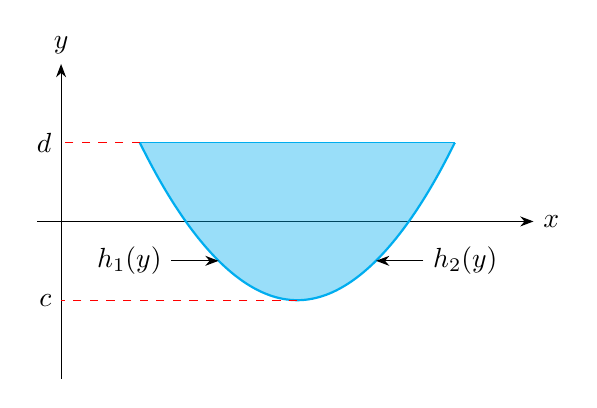
\begin{tikzpicture}[=>stealth]
\draw[-Stealth](-0.3,0)--(6,0)node[right]{$x$};
\draw[-Stealth](0,-2)--(0,2)node[above]{$y$};
\draw[thick,cyan](3,-1)parabola(1,1)
(3,-1)parabola(5,1);
\path[fill=cyan,opacity=0.4](5,1)parabola[bend at end](3,-1)--(3,-1)parabola(1,1)--(1,1)--(5,1)--cycle;
\draw[cyan](1,1)--(5,1);
\draw[red,dashed](3,-1)--(0,-1)
(1,1)--(0,1);
\draw(0,1)node[left]{$d$}
(0,-1)node[left]{$c$}
(4.6,-0.5)node[right]{$h_2(y)$}
(1.4,-0.5)node[left]{$h_1(y)$};
\draw[-Stealth](4.6,-0.5)--(4,-0.5);
\draw[-Stealth](1.4,-0.5)--(2,-0.5);
\end{tikzpicture}
\end{tabular}
\end{table}

The limits of the inner integral may depend on the outer variable; the limits
of the outer integral must be constants.

\begin{exa}
\label{ex:twoparabolas}
Evaluate $\iint_D (x + 2y)\,dA$, where $D$ is the region bounded by the
parabolas $y = 2x^2$ and $y = 1 + x^2$.

\begin{figure}[H]
\centering
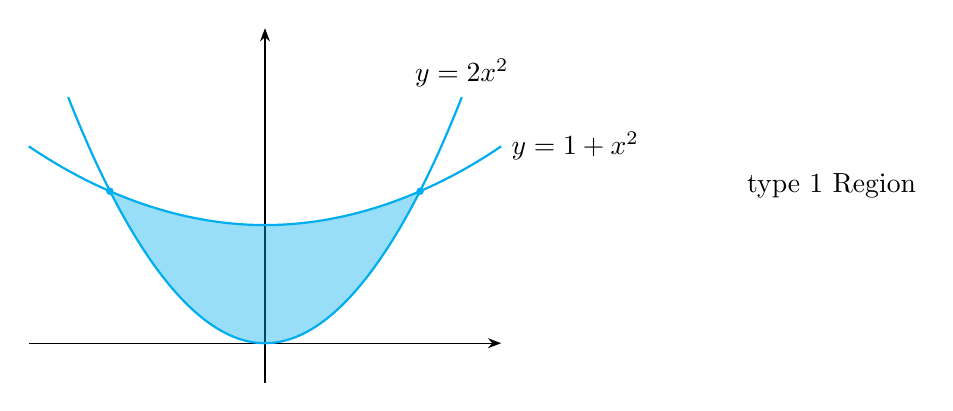
\begin{tikzpicture}[=>stealth]
\draw[-Stealth](-3,0)--(3,0);
\draw[-Stealth](0,-0.5)--(0,4);
\draw[thick,cyan](0,0)parabola(2.5,3.125)node[above,black]{$y=2x^2$}
(0,0)parabola(-2.5,3.125);
\draw[thick,cyan](0,1.5)parabola(3,2.5)node[right,black]{$y = 1 + x^2$}
(0,1.5)parabola(-3,2.5);
\draw(1.97,1.93)node[shape=circle,fill=cyan,scale=0.01cm]{}
(-1.97,1.93)node[shape=circle,fill=cyan,scale=0.01cm]{}
(6,2)node[right]{type 1 Region};
\path[fill=cyan,opacity=0.4](0,0)parabola(1.97,1.93)--(1.97,1.93)parabola[bend at end](0,1.5)--(0,1.5)parabola(-1.97,1.93)--(-1.97,1.93)parabola[bend at end](0,0)--cycle;
\end{tikzpicture}
\end{figure}
\end{exa}

\begin{solution}
The parabolas meet where $2x^2 = 1 + x^2$, that is $x = \pm 1$. Between these,
$2x^2\leq y\leq 1 + x^2$, so $D$ is a type I region and
\begin{align*}
\iint\limits_D (x + 2y)\,dA & = \int^1_{-1}\int^{1 + x^2}_{2x^2} (x + 2y)\,dy\,dx
= \int^1_{-1}\Big[xy + y^2\Big]_{y=2x^2}^{y=1+x^2}dx\\
& = \int^1_{-1}\left(-3x^4 - x^3 + 2x^2 + x + 1\right)dx\\
& = 2\int_0^1\left(-3x^4 + 2x^2 + 1\right)dx = 2\left(-\frac35 + \frac23 +
1\right) = \frac{32}{15},
\end{align*}
the odd terms $-x^3$ and $x$ integrating to zero over $[-1,1]$.
\end{solution}

\begin{exa}
\label{ex:volumeD}
Find the volume of the solid that lies under the paraboloid $z = x^2 + y^2$ and
above the region $D$ in the $xy$-plane bounded by the line $y = 2x$ and the
parabola $y = x^2$.

\begin{figure}[H]
\centering
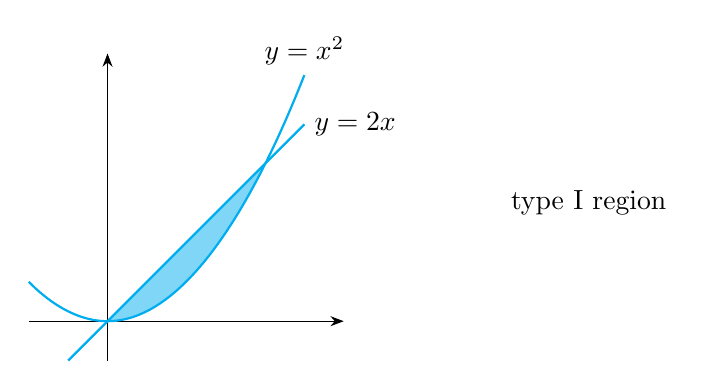
\begin{tikzpicture}[=>stealth]
\draw[-Stealth](-1,0)--(3,0);
\draw[-Stealth](0,-0.5)--(0,3.4);
\draw[thick,cyan](0,0)parabola(2.5,3.125)node[above,black]{$y=x^2$};
\draw[thick,cyan](0,0)parabola(-1,0.5);
\draw[thick,cyan](-0.5,-0.5)--(2.5,2.5)node[right,black]{$y=2x$};
\draw(5,1.5)node[right]{type I region};
\path[fill=cyan,opacity=0.5](0,0)parabola(2,2)--(0,0)--cycle;
\end{tikzpicture}
\end{figure}
\end{exa}

\begin{solution}
The curves meet at $(0,0)$ and $(2,4)$. As a type I region,
\[D = \{ (x,y) \mid  0 \leq x\leq 2,\ x^2 \leq y \leq 2x\},\]
and
\begin{align*}
V & = \int^2_0\int^{2x}_{x^2}(x^2 + y^2)\,dy \,dx = \int^2_0\left[x^2y +
\frac{y^3}{3}\right]_{y=x^2}^{y=2x}dx\\
& = \int^2_0\left( -\frac{x^6}{3} -x^4 +\frac{14 x^3}{3}\right) dx =
-\frac{128}{21} - \frac{32}{5} + \frac{56}{3} = \frac{216}{35}.
\end{align*}

\begin{figure}[H]
\centering
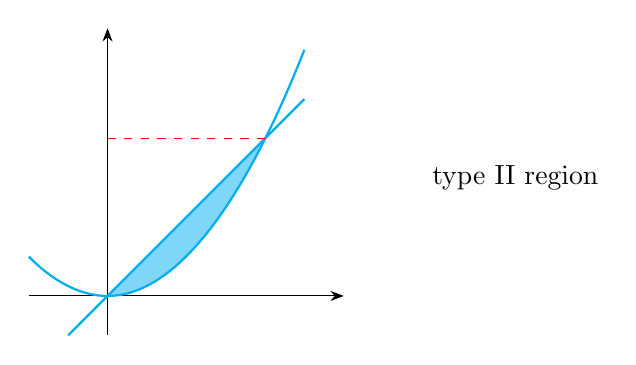
\begin{tikzpicture}[=>stealth]
\draw[-Stealth](-1,0)--(3,0);
\draw[-Stealth](0,-0.5)--(0,3.4);
\draw[thick,cyan](0,0)parabola(2.5,3.125);
\draw[thick,cyan](0,0)parabola(-1,0.5);
\draw[thick,cyan](-0.5,-0.5)--(2.5,2.5);
\draw[dashed,red](0,2)--(2,2);
\draw(4,1.5)node[right]{type II region};
\path[fill=cyan,opacity=0.5](0,0)parabola(2,2)--(0,0)--cycle;
\end{tikzpicture}
\end{figure}

As a type II region, $y = 2x$ gives $x = \frac{y}{2}$ and $y = x^2$ gives
$x = \sqrt y$, so
\[D = \{(x,y) \mid 0\leq y\leq 4,\ \tfrac{y}{2}\leq x \leq \sqrt{y}\},\]
and
\[V = \int^4_0\int^{\sqrt{y}}_{y/2}(x^2 + y^2)\,dx \,dy = \int^4_0\left(
\frac{y^{3/2}}{3} + y^{5/2} - \frac{y^3}{24} - \frac{y^3}{2}\right) dy =
\frac{216}{35},\]
in agreement.
\end{solution}

\begin{exa}
\label{ex:xyline}
Evaluate $\iint_D xy\,dA$, where $D$ is the region bounded by the line
$y = x - 1$ and the parabola $y^2 = 2x + 6$,
\begin{enumerate}
\item regarding $D$ as a type I region, and
\item regarding $D$ as a type II region.
\end{enumerate}

\begin{figure}[H]
\centering
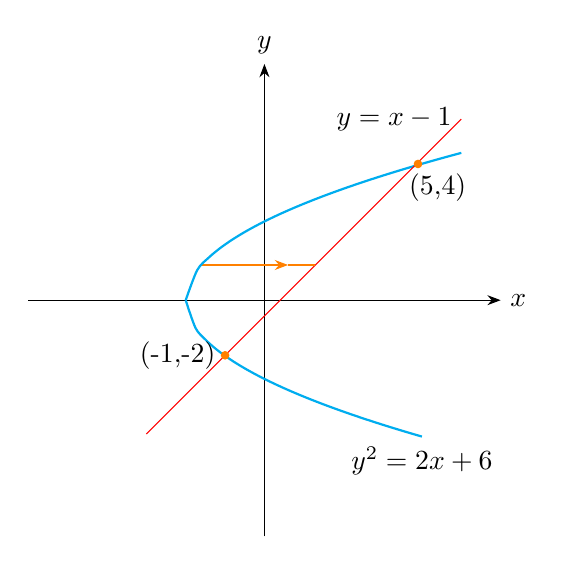
\begin{tikzpicture}[=>stealth]
\draw[-Stealth](-3,0)--(3,0)node[right]{$x$};
\draw[-Stealth](0,-3)--(0,3)node[above]{$y$};
\draw[-Stealth,orange](-0.8,0.447)--(0.3,0.447);
\draw[smooth,domain=-1:2.5,variable=\x,thick, cyan]plot(\x,{sqrt(\x+1)});
\draw[smooth,domain=-1:2,variable=\x,thick,cyan]plot(\x,{-sqrt(\x+1)})node[below,black]{$y^2 = 2x + 6$};
\draw[smooth,domain=-1.5:2.5,variable=\x,red]plot(\x,\x-0.2)node[left,black]{$y = x - 1$};
\draw[orange](0.3,0.447)--(0.647,0.447);
\draw(-0.5,-0.7)node[shape=circle,draw=orange,fill=orange,scale=0.01cm]{}
(1.95,1.73)node[shape=circle,draw=orange,fill=orange,scale=0.01cm]{}
(2.2,1.73)node[below]{(5,4)}
(-0.5,-0.7)node[left]{(-1,-2)};
\end{tikzpicture}
\end{figure}
\end{exa}

\begin{solution}
The curves meet where $(x - 1)^2 = 2x + 6$, that is $x^2 - 4x - 5 = 0$, so at
$(-1,-2)$ and $(5,4)$.
\begin{enumerate}
\item As a type I region, the lower boundary changes at $x = -1$: for
$-3\leq x\leq -1$ the region lies between the two halves of the parabola, and
for $-1\leq x\leq 5$ between the line and the upper half. So
\[\iint\limits_D xy\, dA = \int^{-1}_{-3}\int^{\sqrt{2x + 6}}_{-\sqrt{2x +
6}}xy\,dy\,dx + \int^{5}_{-1}\int^{\sqrt{2x + 6}}_{x - 1}xy\,dy\,dx .\]
The first integral is $0$, since $y$ is odd over a symmetric interval, and the
second is $36$, but two integrals are needed.

\item As a type II region, $D = \{(x,y) \mid -2\leq y\leq 4,\
\frac12 y^2 - 3\leq x\leq y + 1\}$, and a single integral suffices:
\begin{align*}
\iint\limits_D xy\, dA & = \int^4_{-2}\int^{y+1}_{\frac12 y^2-3}xy\,dx\,dy =
\int^4_{-2}\frac{y}{2}\left[(y + 1)^2 - \left(\tfrac12 y^2 - 3\right)^2\right]dy\\
& = \int^4_{-2}\left(-\frac{y^5}{8} + 2y^3 + y^2 - 4y\right) dy = 36 .
\end{align*}
\end{enumerate}
\end{solution}

\begin{exa}
\label{ex:tetrahedron}
Find the volume of the tetrahedron bounded by the planes $x + 2y + z = 2$,
$x = 2y$, $x = 0$ and $z = 0$.

\begin{figure}[H]
\centering
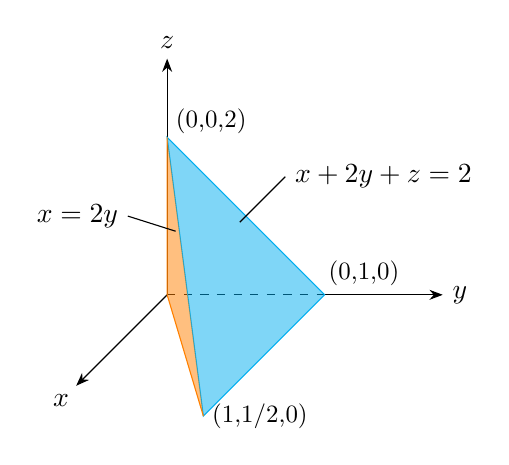
\begin{tikzpicture}[=>stealth]
\draw[-Stealth](2,0,0)--(3.5,0,0)node[right]{$y$};
\draw[-Stealth](0,0,0)--(0,3,0)node[above]{$z$};
\draw[-Stealth](0,0,0)--(0,0,3);
\draw[dashed](0,0,0)--(2,0,0);
\path[fill=cyan,opacity=0.5](2,0,4)--(2,0,0)--(0,2,0)--cycle;
\draw[cyan](2,0,4)--(2,0,0)--(0,2,0)--cycle;
\path[fill=orange,opacity=0.5](2,0,4)--(0,2,0)--(0,0,0)--cycle;
\draw[orange](2,0,4)--(0,0,0)--(0,2,0);
\draw(2,0,4)node[right,scale=0.9]{(1,1/2,0)}
(0,2.2,0)node[right,scale=0.9]{(0,0,2)}
(2.5,0,0)node[above,scale=0.9]{(0,1,0)}
(0,0,3.5)node[]{$x$};
\draw(1,1,0.2)--(1.5,1.5,0)node[right]{$x + 2y + z = 2$}
(0.3,1,0.5)--(-0.5,1,0)node[left]{$x = 2y$};
\end{tikzpicture}
\end{figure}

\begin{figure}[H]
\centering
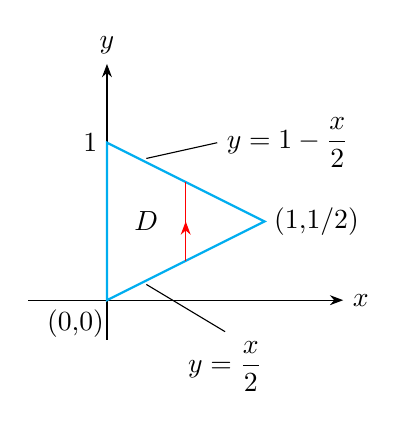
\begin{tikzpicture}[=>stealth]
\draw[-Stealth](-1,0)--(3,0)node[right]{$x$};
\draw[-Stealth](0,-0.5)--(0,3)node[above]{$y$};
\draw[thick,cyan](0,0)--(2,1)--(0,2)--cycle;
\draw(0,2)node[left]{1}
(-0.4,0)node[below]{(0,0)}
(2,1)node[right]{(1,1/2)}
(0.5,1)node[]{$D$};
\draw[red](1,0.5)--(1,1.5);
\draw[red,-Stealth](1,0.5)--(1,1);
\draw(0.5,1.8)--(1.4,2)node[right]{$y = 1 - \dfrac{x}{2}$};
\draw(0.5,0.2)--(1.5,-0.4)node[below]{$y = \dfrac{x}{2}$};
\end{tikzpicture}
\end{figure}
\end{exa}

\begin{solution}
The tetrahedron lies above its base $D$ in the $xy$-plane, the triangle bounded
by $x = 0$, $x = 2y$ and the line $x + 2y = 2$ in which the top face meets
$z = 0$. The lines $x = 2y$ and $x + 2y = 2$ meet at $\left(1,\frac12\right)$,
so
\[D = \left\{(x,y) \mid 0\leq x\leq 1,\ \frac{x}{2}\leq y \leq 1 -
\frac{x}{2}\right\},\]
and the volume lies under $z = 2 - x - 2y$:
\[V = \int^1_0\int^{1 -x/2}_{x/2} ( 2 - x -2y)\,dy\,dx = \int^1_0(x^2 - 2x +
1)\,dx = \frac{1}{3} .\]
\end{solution}

\begin{exa}
\label{ex:reverseorder}
Evaluate the iterated integral $\int^1_0\int^1_{x}\sin (y^2)\,dy\,dx$.

\begin{figure}[H]
\centering
\begin{tikzpicture}[=>stealth]
\draw[-Stealth](-1,0)--(3,0);
\draw[-Stealth](0,-0.5)--(0,3);
\draw[cyan](0,0)--(2.5,2.5)node[above,black]{$y = x$}
(0,2)--(2.5,2)node[right,black]{$y=1$};
\path[fill=cyan,opacity=0.3](0,0)--(2,2)--(0,2)--cycle;
\draw(0,2)node[left]{1}
(2,0)node[below]{1}
(-0.2,0)node[below]{0}
(-2,1)node[left]{(a).}
(6.5,1)node[left]{(b).}
(10,2)node[shape=circle,fill=cyan,scale=0.01cm]{}
(10.2,2)node[below,scale=0.9]{(1,1)};
\draw[dashed,red](2,0)--(2,2);
\draw[-Stealth,red](1,1)--(1,2);
\draw[-Stealth](7.5,0)--(11,0);
\draw[-Stealth](8,-0.5)--(8,3);
\draw[red,-Stealth](8,1)--(8.5,1);
\draw[cyan](8,0)--(10.5,2.5)
(8,2)--(10.5,2);
\path[fill=cyan,opacity=0.3](8,0)--(8,2)--(10,2)--cycle;
\draw[red](8,1)--(9,1);
\end{tikzpicture}
\end{figure}
\end{exa}

\begin{solution}
The inner integral cannot be done in elementary terms, so reverse the order. The
region is $D = \{(x,y)\mid 0\leq x\leq 1,\ x\leq y\leq 1\}$, the triangle with
vertices $(0,0)$, $(0,1)$ and $(1,1)$ shown in (a), which as a type II region,
in (b), is $\{(x,y)\mid 0\leq y\leq 1,\ 0\leq x\leq y\}$. So
\begin{align*}
\int^1_0\int^1_{x}\sin (y^2)\,dy\,dx & = \int^1_0\int^y_{0}\sin (y^2)\,dx\,dy =
\int^1_0y\sin (y^2)\,dy\\
& = \left[-\frac{\cos y^2}{2}\right]_0^1 = \frac{1}{2}(1 - \cos 1)\approx 0.2298 .
\end{align*}
\end{solution}

\begin{exa}
\label{ex:reverseexp}
Reverse the order of integration in $\int_0^4\int_{\sqrt x}^2 e^{y^3}\,dy\,dx$,
and evaluate it.
\end{exa}

\begin{solution}
The region is $0\leq x\leq 4$, $\sqrt x\leq y\leq 2$, which is the same as
$0\leq y\leq 2$, $0\leq x\leq y^2$. So
\[\int_0^4\int_{\sqrt x}^2 e^{y^3}\,dy\,dx = \int_0^2\int_0^{y^2}e^{y^3}\,dx\,dy =
\int_0^2 y^2e^{y^3}\,dy = \frac{e^8 - 1}{3}\approx 993.3 .\]
\end{solution}

\begin{exa}
\label{ex:areaD}
Use a double integral to find the area of the region enclosed by $y = x^2$ and
$y = 8 - x^2$.
\end{exa}

\begin{solution}
The curves meet at $x = \pm 2$. Integrating the constant $1$,
\[A = \int_{-2}^2\int_{x^2}^{8 - x^2}dy\,dx = \int_{-2}^2 (8 - 2x^2)\,dx = 32 -
\frac{32}{3} = \frac{64}{3} .\]
\end{solution}

{\color[wave]{485}\subsection{Properties Of Double Integrals}}

The following properties hold whenever the integrals exist; the first three are
inherited from Riemann sums, and the others follow from them.
\begin{enumerate}
\item $\iint_D \big(f(x,y) + g(x,y)\big)\,dA = \iint_D f(x,y)\,dA +
\iint_D g(x,y)\,dA$.

\item $\iint_D c\, f(x,y)\,dA = c \iint_D f(x,y)\,dA$ for every constant $c$.

\item If $f(x,y)\geq g(x,y)$ for all $(x,y)\in D$, then
$\iint_D f(x,y)\,dA \geq \iint_D g(x,y)\,dA$.

\item If $D = D_1\cup D_2$, where $D_1$ and $D_2$ do not overlap except perhaps
on their boundaries, then
\[\iint\limits_D f(x,y)\,dA  = \iint\limits_{D_1} f(x,y)\,dA  +
\iint\limits_{D_2} f(x,y)\,dA .\]

\item Integrating the constant function $1$ over a region $D$ gives the area of
$D$:
\[\iint\limits_D 1 \,dA = A(D) .\]

\item If $m\leq f(x,y) \leq M$ for all $(x,y) \in D$, then
\[m\,A(D)\leq \iint\limits_D f(x,y)\,dA \leq M\, A(D) .\]
\end{enumerate}
Property 6 follows from properties 3, 2 and 5.

\begin{exa}
\label{ex:estimate}
Use property 6 to estimate $\iint_D e^{\sin x \cos y}\, dA$, where $D$ is the
disc with centre the origin and radius $2$.
\end{exa}

\begin{solution}
Since $-1 \leq \sin x \leq 1$ and $-1 \leq \cos y\leq 1$, we have
$-1 \leq \sin x \cos y\leq 1$, and since the exponential is increasing,
\[\frac{1}{e} \leq e^{\sin x \cos y} \leq e .\]
With $m = \frac{1}{e}$, $M = e$ and $A(D) = \pi (2)^2 = 4\pi$,
\[\frac{4\pi}{e}\leq \iint\limits_D e^{\sin x \cos y}\, dA \leq 4\pi e ,\]
that is, the integral lies between about $4.62$ and $34.2$.
\end{solution}

\begin{exa}
\label{ex:splitregion}
Evaluate $\iint_D |x - y|\,dA$ over the square $D = [0,1]\times[0,1]$.
\end{exa}

\begin{solution}
The integrand changes form across the diagonal $y = x$, so split $D$ by
property 4 into the triangles $D_1$ below the diagonal, where $|x - y| = x - y$,
and $D_2$ above it. By symmetry the two integrals are equal, so
\[\iint\limits_D |x - y|\,dA = 2\int_0^1\int_0^x (x - y)\,dy\,dx =
2\int_0^1\frac{x^2}{2}\,dx = \frac13 .\]
This is the mean distance between two numbers chosen at random in $[0,1]$.
\end{solution}


{\color[wave]{485}\subsection{Double Integrals In Polar Coordinates}}

Suppose that we want to evaluate $\iint_R f(x,y)\,dA$, where $R$ is one of the
regions shown below.

\begin{figure}[H]
\centering
\begin{tikzpicture}[=>stealth]
\draw[-Stealth](-2,0)--(2,0);
\draw[-Stealth](0,-2)--(0,2);
\draw[thick,cyan](0,0)circle[radius=1.5cm];
\path[fill=cyan,opacity=0.4](0,0)circle[radius=1.5cm];
\draw(0.5,0.5)node[]{$R$};
\draw(1,1.2)--(1.5,1.4)node[above]{$x^2 + y^2 = 1$};
\draw[-Stealth](5.5,0)--(10.5,0);
\draw[-Stealth](8,-1)--(8,2.5);
\draw[thick,cyan](9,0)arc[start angle = 0, end angle=180, radius=1];
\draw[thick,cyan](10,0)arc[start angle = 0, end angle = 180, radius =2];
\draw[thick,cyan](6,0)--(7,0)
(9,0)--(10,0);
\draw(9,1)node[above]{$R$}
(-2,1)node[left]{a.}
(5.5,1)node[left]{b.};
\path[fill=cyan,opacity=0.4](9,0)arc[start angle=0,end angle = 180,radius=1]--(7,0)--(6,0)--(6,0)arc[start angle=180, end angle = 0, radius=2]--(10,0)--(9,0)--cycle;
\draw(8.9,0.38)--(9.5,-0.5)node[below]{$x^2 + y^2 = 1$}
(9,1.8)--(10.5,2)node[right]{$x^2 + y^2 = 4$};
\end{tikzpicture}
\end{figure}

\begin{enumerate}
\item[(a)] The disc $x^2 + y^2\leq 1$ is
$\{ (r,\theta) \mid 0 \leq r\leq 1,\ 0 \leq \theta \leq 2\pi \}$.

\item[(b)] The half-annulus between $x^2 + y^2 = 1$ and $x^2 + y^2 = 4$ in the
upper half-plane is $\{ (r,\theta) \mid 1 \leq r\leq 2,\ 0 \leq \theta \leq \pi
\}$.
\end{enumerate}
In either case the description of $R$ in rectangular coordinates is awkward,
but in polar coordinates $R$ is a rectangle in the $r\theta$-plane, a
\emph{polar rectangle}
\[R = \{ (r,\theta) \mid a\leq r\leq b,\ \alpha \leq \theta \leq \beta \},\]
with $a\geq 0$ and $0<\beta - \alpha\leq 2\pi$.

\begin{figure}[H]
\centering
\begin{tikzpicture}[=>stealth]
\draw[-Stealth](-0.3,0)--(4,0)node[right]{$x$};
\draw[-Stealth](0,-0.3)--(0,4)node[above]{$y$};
\draw[thick,cyan](4,2)arc[start angle=30, end angle=75, radius=3cm]
%(3,1.5)arc[start angle=30,end angle=75,radius=2.25cm]
(2.5,1.25)arc[start angle=30,end angle=75,radius=1.85cm]
(0,0)--node[sloped,below,black]{$\theta = \alpha$}(4,2)
(0,0)--node[sloped,above,black]{$\theta = \beta$}(2.18,3.38);
\path[fill=cyan,opacity=0.5](4,2)arc[start angle=30,end angle=75, radius=3cm]--(2.18,3.38)--(1.38,2.1)--(1.38,2.1)arc[start angle = 75, end angle =30,radius=1.85cm]--(2.5,1.25)--(4,2)--cycle;
\coordinate (a) at (0.5,0);
\coordinate (b) at (0,0);
\coordinate (c) at (0.5,0.25);
\coordinate (d) at (0.5,0.775);
\draw
pic[draw=red,thick, angle radius =0.9cm,-Stealth,"$\alpha$"]{angle=a--b--c};
\draw
pic[draw=violet,thick, angle radius=1.4cm,-Stealth]{angle=a--b--d};
\draw(1.3,0.7)node[above]{$\beta$}
(2.5,2.2)node[]{$R$}
(3.3,2.9)node[right]{$r=b$}
(2.3,1.5)node[left]{$r=a$};
\end{tikzpicture}
\end{figure}

Divide $[a,b]$ into $m$ subintervals of width $\Delta r$ and $[\alpha, \beta]$
into $n$ of width $\Delta\theta$. The circles $r = r_i$ and the rays
$\theta = \theta_j$ divide $R$ into small polar rectangles
\[R_{ij} = \{(r,\theta) \mid r_{i-1} \leq r \leq r_i,\ \theta_{j-1}\leq \theta
\leq \theta_j\},\]
and in each we take the centre $(r^*_i, \theta^*_j)$, with
$r_i^* = \frac12(r_{i-1} + r_i)$.

\begin{figure}[H]
\centering
\begin{tikzpicture}[=>stealth]
\draw[-Stealth](-0.3,0)--(4,0)node[right]{$x$};
\draw[-Stealth](0,-0.3)--(0,4)node[above]{$y$};
\draw[thick,cyan](4,2)arc[start angle=30,end angle=75, radius=3cm]
(2.5,1.25)arc[start angle =30, end angle =75, radius=1.85cm]
(2.5,1.25)--(4,2)
(1.38,2.1)--(2.18,3.38);
\draw[red](0,0)--(2.5,1.25)
(0,0)--(1.38,2.1);
\draw[dashed](3,1.5)arc[start angle=30,end angle=75,radius=2.25cm]
(3.5,1.75)arc[start angle=30, end angle=75,radius=2.55cm]
(0,0)--(3.63,2.55)
(0,0)--(2.9,3.1);
\draw(2.7,2.3)node[shape=circle,fill=red,draw=red,scale=0.01cm]{};
\path[fill=olive,opacity=0.4](2.5,1.25)--(4,2)--(4,2)arc[start angle=30,end angle=75,radius=3cm]--(2.18,3.38)--(1.38,2.1)--(1.38,2.1)arc[start angle=75, end angle=30,radius=1.85]--cycle;
\path[fill=orange,opacity=0.4](2.7,1.925)--(3.15,2.2)--(3.15,2.2)arc[start angle=35.087,end angle =46.909,radius=0.5cm]--(2.54,2.7)--(2.18,2.35)--(2.18,2.35)arc[start angle =46.909, end angle = 35.087, radius=0.37cm]--cycle;
\draw[red](2.7,1.9)--(3.16,2.2)
(2.16,2.3)--(2.54,2.7);
\draw(2.75,2.3)--(4,2.7)node[right]{$(r^*_i, \theta^*_j)$}
(2.93,2.05)--(3.5,1.3)node[right]{$\theta_{j-1}$}
(2.35,2.5)--(1.3,3.1)node[left]{$\theta_j$}
(2.5,2.4)--(3.5,3.3)node[above]{$R_{ij}$};
\end{tikzpicture}
\end{figure}

The area of $R_{ij}$ is the difference of two circular sectors of angle
$\Delta\theta$:
\[\Delta A_i = \frac{1}{2}r^2_i\,\Delta \theta - \frac{1}{2}r^2_{i-1}\,\Delta \theta
= \frac{1}{2}(r_i + r_{i-1}) (r_i - r_{i-1})\,\Delta \theta = r^*_{i}\, \Delta r\,
\Delta \theta .\]
So a Riemann sum for $\iint_R f\,dA$ is
\[\sum^m_{i=1}\sum^n_{j=1} f(r^*_i\cos \theta^*_j, r^*_i\sin \theta^*_j)\,
r^*_i\, \Delta r\, \Delta \theta ,\]
which, with $g(r,\theta) = r\, f(r\cos \theta, r \sin \theta)$, is a Riemann sum
for $\int_\alpha^\beta\int_a^b g(r,\theta)\,dr\,d\theta$. Passing to the limit
gives the following.

\begin{thm}[Double integrals in polar coordinates]
\label{thm:polar}
If $f$ is continuous on a polar rectangle
$R = \{ (r,\theta) \mid a\leq r\leq b,\ \alpha \leq \theta \leq \beta \}$, where
$0\leq\beta - \alpha\leq 2\pi$, then
\[\iint\limits_R f(x,y)\,dA = \int^{\beta}_{\alpha} \int^b_a f(r\cos \theta,
r\sin \theta)\, r\, dr\, d\theta .\]
More generally, if $D = \{(r,\theta)\mid \alpha\leq\theta\leq\beta,\
h_1(\theta)\leq r\leq h_2(\theta)\}$, then
\[\iint\limits_D f(x,y)\,dA = \int^{\beta}_{\alpha}
\int^{h_2(\theta)}_{h_1(\theta)} f(r\cos \theta, r\sin \theta)\, r\, dr\,
d\theta .\]
\end{thm}

In practice: write $x = r\cos\theta$, $y = r\sin\theta$, replace $dA$ by
$r\,dr\,d\theta$, and use the polar limits. Forgetting the factor $r$ is the
commonest error; the subsection on change of variables shows that it is a
Jacobian.

\begin{exa}
\label{ex:polarannulus}
Evaluate $\iint_R (3x + 4y^2) \,dA$, where $R$ is the region in the upper
half-plane bounded by the circles $x^2 + y^2 = 1$ and $x^2 + y^2 = 4$.
\end{exa}

\begin{solution}
Here $R = \{ (r,\theta) \mid 1 \leq r \leq 2,\ 0\leq \theta \leq \pi\}$, so
\begin{align*}
\iint\limits_R (3x + 4y^2) \,dA & = \int^{\pi}_0\int^2_1(3r\cos \theta + 4r^2\sin^2
\theta )\, r\,dr\,d\theta = \int^{\pi}_0\Big[r^3\cos\theta +
r^4\sin^2\theta\Big]_{r=1}^{r=2}d\theta\\
& = \int^{\pi}_0\left(7\cos \theta + \frac{15}{2}( 1 - \cos 2\theta )\right)
d\theta = \frac{15\pi}{2} .
\end{align*}
\end{solution}

\begin{exa}
\label{ex:polarvolume}
Find the volume of the solid bounded by the plane $z = 0$ and the paraboloid
$z = 1-x^2 -y^2$.

\begin{figure}[H]
\centering
\begin{tikzpicture}[=>stealth]
\draw[dashed](-2,0,0)--(2,0,0)
(0,0,0)--(0,2,0)
(0,0,0)--(0,0,1)
(0,0,0)--(0,0,-1);
\draw[-Stealth](0,2,0)--(0,3,0);
\draw[-Stealth](2,0,0)--(3,0,0);
\draw[-Stealth](0,0,1)--(0,0,3);
\draw(-3,0,0)--(-2,0,0);
\draw[teal](0,2)parabola(2,0)
(0,2)parabola(-2,0);
\draw[teal](-2,0)arc(180:360:2cm and 0.5cm);
\draw[dashed,teal](2,0)arc(0:180:2cm and 0.5cm);
\path[fill=teal,opacity=0.4](0,0)circle(2cm and 0.5cm)--(2,0)parabola[bend at end](0,2)--(0,2)parabola(-2,0);
\draw(0.5,0,0.6)node[right]{$D$};
\draw(0,2.2,0)node[right]{(0,0,1)};
\end{tikzpicture}
\end{figure}
\end{exa}

\begin{solution}
The paraboloid meets the plane $z = 0$ in the circle $x^2 + y^2 = 1$, so the
solid lies above the unit disc $D$, and
\[V = \iint\limits_D (1-x^2-y^2)\,dA = \int^{2\pi}_0\int^1_0 ( 1 - r^2)\, r\,dr\,
d\theta = 2\pi\left[\frac{r^2}{2} - \frac{r^4}{4}\right]_0^1 = \frac{\pi}{2} .\]
In rectangular coordinates the same integral would need the limits
$\pm\sqrt{1 - x^2}$ and a much harder calculation.
\end{solution}

\begin{exa}
\label{ex:gaussian}
Evaluate $\iint_D e^{-(x^2 + y^2)}\,dA$ over the disc of radius $a$, and deduce
that $\int_{-\infty}^\infty e^{-x^2}\,dx = \sqrt\pi$.
\end{exa}

\begin{solution}
In polar coordinates,
\[\iint\limits_{D_a} e^{-(x^2+y^2)}\,dA = \int_0^{2\pi}\int_0^a e^{-r^2}r\,dr\,
d\theta = 2\pi\left[-\frac{e^{-r^2}}{2}\right]_0^a = \pi\left(1 -
e^{-a^2}\right),\]
which tends to $\pi$ as $a\to\infty$. Over the whole plane the integral is
therefore $\pi$. But computed over the square $[-a,a]^2$ and then letting
$a\to\infty$, which gives the same limit since the squares and discs are nested
between each other, it factors as
$\left(\int_{-a}^a e^{-x^2}dx\right)\left(\int_{-a}^a e^{-y^2}dy\right)$. So
$\left(\int_{-\infty}^\infty e^{-x^2}dx\right)^2 = \pi$, and the integral is
$\sqrt\pi$. This integral, central to probability, cannot be found by any
single-variable method.
\end{solution}

\begin{exa}
\label{ex:rose}
Find the area enclosed by one loop of the four-leaved rose $r = \cos 2\theta$.
\end{exa}

\begin{solution}
One loop is traced as $\theta$ runs from $-\frac{\pi}{4}$ to $\frac{\pi}{4}$, so
\[A = \int_{-\pi/4}^{\pi/4}\int_0^{\cos 2\theta}r\,dr\,d\theta =
\int_{-\pi/4}^{\pi/4}\frac{\cos^2 2\theta}{2}\,d\theta =
\frac14\int_{-\pi/4}^{\pi/4}(1 + \cos 4\theta)\,d\theta = \frac{\pi}{8} .\]
\end{solution}

\begin{exa}
\label{ex:sphereincylinder}
Find the volume of the solid that lies inside the sphere $x^2 + y^2 + z^2 = 4$
and outside the cylinder $x^2 + y^2 = 1$.
\end{exa}

\begin{solution}
Above each point of the annulus $1\leq r\leq 2$ the solid extends from
$z = -\sqrt{4 - r^2}$ to $z = \sqrt{4 - r^2}$, so
\[V = \int_0^{2\pi}\int_1^2 2\sqrt{4 - r^2}\,r\,dr\,d\theta = 2\pi\left[-\frac23(4
- r^2)^{3/2}\right]_1^2 = 2\pi\cdot\frac23\cdot 3^{3/2} = 4\sqrt3\,\pi\approx
21.8 .\]
\end{solution}

{\color[wave]{485}\subsection{Applications Of Double Integrals}}

Double integrals compute volumes and areas, as already seen, and also masses,
charges, moments, centres of mass, moments of inertia, probabilities and
expected values: any quantity that is a density integrated over a region.

\subhead{Mass and Charge}

Suppose that a lamina (a thin flat plate) occupies a region $D$ of the
$xy$-plane and has density $\rho (x,y)$, in units of mass per unit area. A small
rectangle of area $\Delta A$ about $(x^*_{ij},y^*_{ij})$ has mass about
$\rho(x^*_{ij},y^*_{ij})\,\Delta A$, so the total mass of the lamina is
\[m = \lim_{k,l\to \infty} \sum^k_{i=1}\sum^l_{j=1} \rho (x_{ij}^*,y^*_{ij})\,
\Delta A = \iint\limits_D \rho (x,y)\,dA .\]
In the same way, if an electric charge is distributed over $D$ with charge
density $\sigma (x,y)$, the total charge is
\[Q = \iint\limits_D \sigma (x,y)\,dA .\]

\begin{exa}
\label{ex:charge}
Charge is distributed over the triangular region $D$ with vertices $(1,0)$,
$(1,1)$ and $(0,1)$ so that the charge density at $(x,y)$ is
$\sigma(x,y) = xy$ coulombs per square metre. Find the total charge.

\begin{figure}[H]
\centering
\begin{tikzpicture}[=>stealth]
\draw[-Stealth](-0.5,0)--(4,0);
\draw[-Stealth](0,-0.5)--(0,2.5);
\draw[thick,cyan](0,1.5)--(1.5,1.5);
\draw[thick,cyan](1.5,0)--(0,1.5);
\draw[thick,cyan](1.5,0)--(1.5,1.5);
\draw(1.5,0)node[below]{(1,0)}
(0,1.5)node[left]{(0,1)}
(1.5,1.5)node[right]{(1,1)}
(1.05,1.05)node[]{$D$};
\path[fill=brown,opacity=0.5](1.5,0)--(1.5,1.5)--(0,1.5)--cycle;
\end{tikzpicture}
\end{figure}
\end{exa}

\begin{solution}
The region is bounded by $y = 1 - x$ below, $y = 1$ above, and $x = 1$ on the
right, so
\[Q = \int^1_0\int^1_{1-x} xy\,dy\,dx = \int_0^1 \frac{x}{2}\left(1 -
(1-x)^2\right)dx = \int_0^1\left(x^2 - \frac{x^3}{2}\right)dx = \frac13 -
\frac18 = \frac{5}{24}\ \text{C}.\]
\end{solution}

\subhead{Moments and Centre of Mass}

For point masses $m_1,\dots, m_n$ at $(x_1,y_1),\dots, (x_n,y_n)$, the moments
about the $y$- and $x$-axes are
\[M_y = \sum_{i=1}^n m_ix_i ,\qquad M_x = \sum_{i=1}^n m_iy_i ,\]
and the centre of mass is $(\bar x,\bar y)$ with
\[\bar x = \frac{M_y}{m} , \qquad \bar y = \frac{M_x}{m} ,\qquad m =
\sum^n_{i=1} m_i .\]
For a lamina with density $\rho (x,y)$, the sums become integrals:
\[M_x = \iint\limits_D y \, \rho(x,y)\,dA ,\qquad M_y = \iint\limits_D x \,
\rho(x,y)\,dA ,\qquad \bar x = \frac{M_y}{m},\qquad \bar y = \frac{M_x}{m} .\]
The centre of mass is the point at which the lamina would balance. For constant
density it depends only on the shape of $D$, and is called the
\emph{centroid}.

\begin{exa}
\label{ex:centremass}
Find the mass and centre of mass of a triangular lamina with vertices $(0,0)$,
$(1,0)$ and $(0,2)$ if the density is $\rho (x,y) = 1 + 3x + y$.
\end{exa}

\begin{solution}

\begin{figure}[H]
\centering
\begin{tikzpicture}[=>stealth]
\draw[-Stealth](-0.5,0)--(3,0)node[right]{$x$};
\draw[-Stealth](0,-0.5)--(0,4)node[above]{$y$};
\draw[thick,cyan](2,0)--(0,3);
\draw[cyan,thick](0,0)--(0,3);
\draw[thick,cyan](0,0)--(2,0);
\path[fill=cyan,opacity=0.3](0,0)--(2,0)--(0,3)--cycle;
\draw(2,0)node[below]{$(1,0)$}
(-0.4,0)node[below]{(0,0)}
(0,3)node[left]{$(0,2)$}
(1,1)node[left]{$D$};
\draw(1.1,1.5)--(2,2)node[right]{$y= 2-2x$};
\end{tikzpicture}
\end{figure}

The hypotenuse is $y = 2 - 2x$, so
\[m = \int^1_0 \int^{2-2x}_0(1 + 3x + y)\, dy \, dx = \int_0^1 \left(4 -
4x^2\right)dx = \frac{8}{3} .\]
Then
\begin{align*}
\bar x & = \frac{3}{8}\int^1_0 \int^{2 - 2x}_0 x(1 + 3x + y)\,dy\,dx =
\frac38\int_0^1\left(4x - 4x^3\right)dx = \frac38\cdot 1 = \frac{3}{8},\\
\bar y & = \frac{3}{8}\int^1_0 \int^{2 - 2x}_0 y(1 + 3x + y)\,dy\,dx =
\frac38\cdot\frac{11}{6} = \frac{11}{16} .
\end{align*}
The centre of mass is $\left(\frac38,\frac{11}{16}\right)$. The centroid of the
triangle is $\left(\frac13,\frac23\right)$; the density, larger towards the
right, moves the balance point to the right.
\end{solution}

\begin{exa}
\label{ex:semicircle}
Find the centroid of the half-disc $x^2 + y^2\leq a^2$, $y\geq 0$.
\end{exa}

\begin{solution}
By symmetry $\bar x = 0$. With $\rho = 1$, the mass is the area
$\frac{\pi a^2}{2}$, and in polar coordinates
\[M_x = \int_0^\pi\int_0^a r\sin\theta\cdot r\,dr\,d\theta = \frac{a^3}{3}\int_0^\pi
\sin\theta\,d\theta = \frac{2a^3}{3},\qquad \bar y = \frac{2a^3/3}{\pi a^2/2} =
\frac{4a}{3\pi}\approx 0.424\,a .\]
\end{solution}

\subhead{Moments of Inertia}

The \emph{moment of inertia} of a particle of mass $m$ about an axis is $mr^2$,
where $r$ is its distance from the axis; it measures resistance to rotation, as
mass measures resistance to linear motion. For a lamina,
\[I_x = \iint\limits_D y^2\rho(x,y)\,dA,\qquad I_y = \iint\limits_D
x^2\rho(x,y)\,dA,\qquad I_0 = \iint\limits_D (x^2 + y^2)\rho(x,y)\,dA,\]
about the $x$-axis, the $y$-axis and the origin, with $I_0 = I_x + I_y$.

\begin{exa}
\label{ex:inertiadisc}
Find the moment of inertia about its centre of a uniform disc of density $\rho$
and radius $a$, and express it in terms of the mass $m$.
\end{exa}

\begin{solution}
\[I_0 = \int_0^{2\pi}\int_0^a r^2\rho\,r\,dr\,d\theta = 2\pi\rho\frac{a^4}{4} =
\frac{\pi\rho a^4}{2} .\]
Since $m = \rho\pi a^2$, $I_0 = \frac12 ma^2$: a disc is easier to spin than a
ring of the same mass and radius, for which $I_0 = ma^2$, because its mass is
closer to the centre.
\end{solution}

\subhead{Probability}

A \emph{joint density function} of two random variables $X$ and $Y$ is a
function $f\geq 0$ with $\iint_{\mathbb{R}^2}f\,dA = 1$, and the probability that
$(X,Y)$ lies in a region $D$ is $\iint_D f(x,y)\,dA$.

\begin{exa}
\label{ex:jointdensity}
The joint density of $X$ and $Y$ is $f(x,y) = C(x + 2y)$ for
$0\leq x\leq 10$, $0\leq y\leq 10$, and $0$ elsewhere. Find $C$ and
$P(X\leq 7,\ Y\geq 2)$.
\end{exa}

\begin{solution}
The total probability is
$C\int_0^{10}\int_0^{10}(x + 2y)\,dy\,dx = C\int_0^{10}(10x + 100)\,dx = 1500C$,
so $C = \frac{1}{1500}$. Then
\begin{align*}
P(X\leq 7,\ Y\geq 2) & = \frac{1}{1500}\int_0^7\int_2^{10}(x + 2y)\,dy\,dx =
\frac{1}{1500}\int_0^7 (8x + 96)\,dx\\
& = \frac{196 + 672}{1500} = \frac{868}{1500}\approx 0.579 .
\end{align*}
\end{solution}


{\color[wave]{485}\subsection{Triple Integrals}}

Suppose that $f$ is defined on a rectangular box
\[B = \{(x,y,z) \mid a\leq x \leq b,\ c\leq y \leq d,\ r\leq z \leq s\} .\]
Divide $[a,b]$ into $l$ subintervals of width $\Delta x$, $[c,d]$ into $m$ of
width $\Delta y$, and $[r,s]$ into $n$ of width $\Delta z$. The planes through
the division points cut $B$ into $lmn$ sub-boxes
\[B_{ijk} = [x_{i-1},x_i]\times [y_{j-1},y_j] \times [z_{k-1},z_k],\]
each of volume $\Delta V = \Delta x\,\Delta y\,\Delta z$.

\begin{figure}[H]
\centering
\begin{tikzpicture}[=stealth]
\draw[-Stealth](3,0,0)--(4,0,0);
\draw[-Stealth](0,1,0)--(0,2,0);
\draw[-Stealth](0,0,2)--(0,0,3);
\draw[dashed,thick,cyan](0,0,2)--(0,0,0)--(3,0,0)
(0,0,0)--(0,1,0);
\draw[thick,cyan](3,0,2)--(3,1,2)--(3,1,0)--(0,1,0)--(0,1,2)--(3,1,2)--(3,0,2)
(0,0,2)--(0,1,2)
(3,0,0)--(3,1,0)
(0,0,2)--(3,0,2)--(3,0,0);
\path[fill=cyan,opacity=0.3](0,0,0)--(3,0,0)--(3,0,2)--(0,0,2)--(0,0,0)--(0,1,0)--(3,1,0)--(3,0,0)--(0,0,0)--(0,1,0)--(0,1,2)--(0,0,2);
\end{tikzpicture}
\end{figure}

Choosing a sample point $(x^*_{ijk}, y^*_{ijk},z^*_{ijk})$ in each $B_{ijk}$
gives the \emph{triple Riemann sum}
\[\sum^l_{i=1} \sum^m_{j=1} \sum^n_{k=1} f(x^*_{ijk}, y_{ijk}^*,
z^*_{ijk})\,\Delta V .\]

\begin{defn}
\label{defn:tripleintegral}
The \emph{triple integral} of $f$ over the box $B$ is
\[\iiint\limits_B f(x,y,z)\,dV = \lim_{l,m,n\to \infty} \sum^l_{i=1}
\sum^m_{j=1} \sum^n_{k=1} f(x^*_{ijk}, y_{ijk}^*, z^*_{ijk})\,\Delta V\]
if the limit exists.
\end{defn}

If $f$ is a density, in mass per unit volume, the triple integral is the total
mass of the solid; if $f = 1$, it is the volume of $B$.

{\color[wave]{485}\subsection{Fubini's Theorem for Triple Integrals}}

\begin{thm}[Fubini's theorem for triple integrals]
\label{thm:fubini3}
If $f$ is continuous on the rectangular box $B = [a,b]\times [c,d] \times [r,s]$,
then
\[\iiint\limits_B f(x,y,z)\,dV = \int^s_r\int^d_c\int^b_a f(x,y,z)\,dx \,dy
\,dz ,\]
and the iterated integral may be taken in any of the six possible orders.
\end{thm}

\begin{exa}
\label{ex:triplebox}
Evaluate $\iiint_B xyz^2\, dV$, where
$B = \{ (x,y,z) \mid 0\leq x\leq 1,\ -1 \leq y \leq 2,\ 0\leq z\leq 3\}$.
\end{exa}

\begin{solution}
The integrand is a product of functions of one variable each, so the integral
factors:
\[\iiint\limits_B xyz^2\, dV = \int^1_0 x\,dx\int^2_{-1}y\,dy\int^3_0 z^2\,dz =
\frac12\cdot\frac32\cdot 9 = \frac{27}{4} .\]
\end{solution}

\begin{exa}
\label{ex:tripleboxexp}
Evaluate $\iiint_B (x + y)e^{z}\,dV$ over $B = [0,1]\times[0,2]\times[0,\ln 2]$.
\end{exa}

\begin{solution}
Integrating $z$ first, $\int_0^{\ln 2}e^z\,dz = 1$, so the integral is
$\int_0^1\int_0^2 (x + y)\,dy\,dx = \int_0^1 (2x + 2)\,dx = 3$.
\end{solution}

{\color[wave]{485}\subsection{Triple Integrals Over A General Bounded Region $E$}}

To integrate over a general bounded solid $E$, enclose $E$ in a box $B$ and
define $F$ to agree with $f$ on $E$ and to be $0$ at the points of $B$ outside
$E$. Then
\[\iiint\limits_E f(x,y,z)\, dV = \iiint\limits_B F(x,y,z)\,dV .\]

A solid region $E$ is of \emph{type 1} if it lies between the graphs of two
continuous functions of $x$ and $y$,
\[E = \{ (x,y,z) \mid (x,y) \in D,\ u_1(x,y) \leq z \leq u_2(x,y)\},\]
where $D$ is the projection of $E$ on the $xy$-plane.

\begin{figure}[H]
\centering
\begin{tikzpicture}[=>stealth]
\draw[-Stealth](0,0,0)--(3,0,0)node[right]{$y$};
\draw[-Stealth](0,0,0)--(0,4,0)node[above]{$z$};
\draw[-Stealth](0,0,0)--(0,0,3);
\draw(0,0,3.5)node[]{$x$};
\draw[cyan,thick](3,3,2)arc(360:180:1cm and 0.3cm)
(1,3,2)parabola(1.8,3,1.8)
(1.8,3,1.8)parabola(3,3,2)
(2,1.8,2.3)--(2,2.8,2.3)
(1,2,2)--(1,3,2)
(3,2,2)--(3,3,2);
%(2,2.2,1.7)--(2,3,1.7);
\path[fill=cyan,opacity=0.5](3,3,2)arc(360:180:1cm and 0.3cm)--(1,3,2)--(1,2,2)--(1,2,2)arc(180:360:1cm and 0.3cm)--(3,2,2)--(3,3,2)--cycle;
\path[fill=cyan,opacity=0.5](3,3,2)arc(360:180:1cm and 0.3cm)--(1,3,2)parabola(1.8,3,1.8)--(1.8,3,1.8)parabola(3,3,2)--cycle;
%%
\draw[cyan,dashed,thick](3,2,2)arc(0:180:1cm and 0.3cm);
\draw[cyan,thick](1,2,2)arc(180:360:1cm and 0.3cm);
%%%%%
\draw[orange](3,0,2)arc(0:360:1cm and 0.3cm);
\path[fill=orange,opacity=0.5](3,0,2)arc(0:360:1cm and 0.3cm);
\draw(2,0,2)node[]{$D$};
%%%
\draw[red,dashed](1,0,2)--(1,2,2)
(3,0,2)--(3,2,2);
\draw[-Stealth](2,2.5,-0.5)--(1.5,2,-0.5);
\draw[-Stealth](3,1.5)parabola[bend at end](1.8,1.1);
\draw(2,2.5,-0.5)node[right]{$z=u_2(x,y)$}
(3,1.5)node[right]{$z=u_1(x,y)$};
\end{tikzpicture}
\end{figure}

\subhead{Type 1 Solids}

For a type 1 solid, Fubini's theorem gives
\[\iiint\limits_E f(x,y,z)\,dV = \iint\limits_D \left[
\int^{u_2(x,y)}_{u_1(x,y)} f(x,y,z)\,dz\right] dA .\]
If moreover the projection $D$ is a type I plane region,
\[E = \{(x,y,z) \mid a\leq x \leq b,\ g_1(x)\leq y\leq g_2(x),\ u_1(x,y)\leq
z\leq u_2(x,y)\},\]
then
\[\iiint\limits_E f(x,y,z)\,dV = \int^b_a \int^{g_2(x)}_{g_1(x)}
\int^{u_2(x,y)}_{u_1(x,y)} f(x,y,z)\,dz\,dy\,dx .\]

\begin{figure}[H]
\centering
\begin{tikzpicture}[=>stealth]
\draw[-Stealth](-0.3,0,0)--(4,0,0)node[right]{$y$};
\draw[-Stealth](-0.3,0,0)--(-0.3,4,0)node[above]{$z$};
\draw[-Stealth](-0.3,0,0)--(-0.3,0,3.5);
\draw(-0.3,0,4)node[]{$x$};
\draw[orange](1,0,1)--(1,0,3)
(1,0,1)parabola(2.5,0,1.8)
(1,0,3)parabola(2.5,0,2.5)
(2.5,0,1.8)--(2.5,0,2.5);
\draw(1.1,0,1.8)node[right]{$D$}
(2.7,0,3.5)node[right]{$h_2(y)$}
(2.7,0,1)node[right]{$h_1(y)$};
\path[fill=orange,opacity=0.4](1,0,1)--(1,0,3)--(1,0,3)parabola(2.5,0,2.5)--(2.5,0,2.5)--(2.5,0,1.8)--(2.5,0,1.8)parabola[bend at end](1,0,1)--cycle;
\draw[-Stealth](2.7,0,3.5)parabola(1.8,0,2.8);
\draw[-Stealth](2.7,0,1)parabola(1.8,0,1.2);
%%
\draw[dashed,red]
(1,0,1)--(1,2,1)
(1,0,3)--(1,2,3)
(2.5,0,1.8)--(2.5,2,1.8)
(2.5,0,2.5)--(2.5,2,2.5);
%%
\draw[thick,cyan]%(1,2,1)--(1,2,3)
%(1,2,1)parabola(2.5,2,1.8)
(1,2,3)parabola(2.5,2,2.5)
(2.5,2,1.8)--(2.5,2,2.5);
%%
\draw[thick,cyan](1,3,1)--(1,3,3)
(1,3,1)parabola(2.5,3,1.8)
(1,3,3)parabola(2.5,3,2.5)
(2.5,3,1.8)--(2.5,3,2.5)
%
%(1,2,1)--(1,3,1)
(1,2,3)--(1,3,3)
(2.5,2,1.8)--(2.5,3,1.8)
(2.5,2,2.5)--(2.5,3,2.5);
\draw[thick,cyan,dashed](1,2,1)--(1,3,1)
(1,2,1)parabola(2.5,2,1.8)
(1,2,1)--(1,2,3);
\path[fill=cyan,opacity=0.4](1,3,1)--(1,3,3)--(1,3,3)parabola(2.5,3,2.5)--(2.5,3,2.5)--(2.5,3,1.8)--(2.5,3,1.8)parabola[bend at end](1,3,1)--cycle;
\path[fill=cyan,opacity=0.4](1,2,3)parabola(2.5,2,2.5)--(2.5,2,2.5)--(2.5,2,1.8)--(2.5,3,1.8)--(2.5,3,2.5)parabola[bend at end](1,3,3)--(1,2,3)--cycle;
%%
\draw[-Stealth](1.8,2.9,-0.2)--(1.2,2.3,0);
\draw[-Stealth](2,1.5,-0.5)parabola[bend at end](1,1,-0.2);
\draw(2,2.8,-0.2)node[above]{$u_2(x,y)$}
(2,1.5,-0.5)node[right]{$u_1(x,y)$};
\end{tikzpicture}
\end{figure}

If instead $D$ is a type II plane region,
\[E = \{(x,y,z) \mid c\leq y \leq d,\ h_1(y)\leq x \leq h_2(y),\ u_1(x,y) \leq
z \leq u_2(x,y) \},\]
then
\[\iiint\limits_E f(x,y,z)\,dV = \int^d_c \int^{h_2(y)}_{h_1(y)}
\int^{u_2(x,y)}_{u_1(x,y)} f(x,y,z)\,dz\,dx\,dy .\]

\begin{exa}
\label{ex:tetraz}
Evaluate $\iiint_E z \, dV$, where $E$ is the tetrahedron bounded by the planes
$x = 0$, $y = 0$, $z = 0$ and $x + y + z = 1$.

\begin{figure}[H]
\centering
\begin{tikzpicture}[=>stealth]
\draw[-Stealth](2,0,0)--(4,0,0)node[right]{$y$};
\draw[-Stealth](0,2,0)--(0,3,0)node[above]{$z$};
\draw[-Stealth](0,0,2)--(0,0,3.5);
\draw(0,0,3.9)node[]{$x$}
(2,0,0)node[shape=circle,fill=cyan,draw=cyan,thick,scale=0.01cm]{}
(0,2,0)node[shape=circle,fill=cyan,draw=cyan,thick,scale=0.01cm]{}
(0,0,2)node[shape=circle,fill=cyan,draw=cyan,thick,scale=0.01cm]{};
\draw[dashed](-1,0,0)--(2,0,0)
(0,-0.5,0)--(0,2,0)
(0,0,-0.5)--(0,0,2);
\draw[thick,cyan](2,0,0)--(0,2,0)--(0,0,2)--cycle;
\path[fill=cyan,opacity=0.4](2,0,0)--(0,2,0)--(0,0,2)--cycle;
\draw(2.5,0,0)node[above]{(0,1,0)}
(0,0,2.9)node[right]{(1,0,0)}
(0,2,0)node[left]{(0,0,1)};
\draw(1,1,0.5)--(2,2,0)node[above]{$x + y + z = 1$};
\draw[-Stealth](7.5,0)--(11,0)node[right]{$x$};
\draw[-Stealth](8,-0.5)--(8,3)node[above]{$y$};
\draw[thick,teal](10,0)--(8,2);
\path[fill=teal,opacity=0.3](8,0)--(10,0)--(8,2)--cycle;
\draw(8,2)node[left]{(0,1)}
(10,0)node[below]{(1,0)};
\draw[thick,red,-Stealth](9,0)--(9,0.5);
\draw[thick,red](9,0.5)--(9,1);
\draw(8.5,1.6)--(9,2)node[right]{$y = 1 -x$};
\end{tikzpicture}
\end{figure}
\end{exa}

\begin{solution}
The lower boundary is $z = 0$ and the upper the plane $z = 1 - x - y$, over the
triangle $D$ in the $xy$-plane bounded by the axes and the line $y = 1 - x$.
So
\begin{align*}
\iiint\limits_E z\,dV & = \int^1_0 \int_0^{1-x}\int^{1-x-y}_0 z \,dz \,dy\, dx =
\frac{1}{2} \int^1_0 \int_0^{1-x}(1 - x- y)^2 \,dy \,dx\\
& = \frac16\int_0^1(1 - x)^3\,dx = \frac{1}{24} .
\end{align*}
\end{solution}

The other two coordinate directions give two more types. A solid $E$ is of
\emph{type 2} if
\[E = \{ (x,y,z) \mid (y,z)\in D,\ u_1(y,z) \leq x \leq u_2(y,z)\},\]
where $D$ is the projection of $E$ on the $yz$-plane, bounded in front and
behind by the surfaces $x = u_1(y,z)$ and $x = u_2(y,z)$.

\begin{figure}[H]
\centering
\begin{tikzpicture}[=>stealth]
\draw[-Stealth](0,0,0)--(4,0,0)node[right]{$y$};
\draw[-Stealth](0,0,0)--(0,2,0)node[above]{$z$};
\draw[-Stealth](0,0,0)--(0,0,4);
\draw(0,0,4.5)node[]{$x$};
\draw[cyan](3,0,1.5)arc(0:180:1cm and 0.5cm)
(3,0,3.5)arc(0:360:1cm and 0.5cm);
\draw[dashed,cyan](1,0,1.5)parabola(1.8,-0.2,1.5)
(3,0,1.5)parabola[bend at end](1.8,-0.2,1.5);
\path[fill=cyan,opacity=0.4](3,0,3.5)arc(0:180:1cm and 0.5cm)--(1,0,3.5)--(1,0,1.5)--(1,0,1.5)arc(180:0:1cm and 0.5cm)--(3,0,1.5)--(3,0,3.5)--cycle;
\path[fill=cyan,opacity=0.4](1,0,3.5)arc(180:360:1cm and 0.5cm)--(3,0,3.5)--(3,0,1.5)--(3,0,1.5)parabola[bend at end](1.8,-0.2,1.5)--(1.8,-0.2,1.5)parabola[bend at end](1,0,1.5)--(1,0,1.5)--(1,0,3.5)--cycle;
\path[fill=cyan,opacity=0.4](3,0,3.5)arc(0:360:1cm and 0.5cm)
(3,0,1.5)arc(0:180:1cm and 0.5cm)--(1,0,1.5)parabola(1.8,-0.2,1.5)--(1.8,-0.2,1.5)parabola(3,0,1.5)--cycle;;
\draw[orange](3,0,-1)arc(0:180:1cm and 0.5cm)
(1,0,-1)parabola(1.8,-0.2,-1)
(3,0,-1)parabola[bend at end](1.8,-0.2,-1);
\path[fill=orange,opacity=0.4](3,0,-1)arc(0:180:1cm and 0.5cm)--(1,0,-1)parabola(1.8,-0.2,-1)--(1.8,-0.2,-1)parabola(3,0,-1)--cycle;
\draw[dashed,red](3,0,1.5)--(3,0,-1)
(1,0,0.5)--(1,0,-1);
\draw(2,-0.2,-1)node[above]{$D$}
(3.5,-0.3,4)node[right]{$x=u_2(y,z)$}
(3.5,-0.5,0.3)node[right]{$x=u_1(y,z)$}; 
\draw[-Stealth](3.5,-0.3,4)parabola(2.6,0,3.5);
\draw[-Stealth](3.5,-0.5,0.3)parabola[bend at end](2.4,0,1);
\end{tikzpicture}
\end{figure}

Then
\[\iiint\limits_E f(x,y,z)\,dV = \iint\limits_D \left[
\int^{u_2(y,z)}_{u_1(y,z)} f(x,y,z)\,dx\right] dA .\]
A solid $E$ is of \emph{type 3} if
\[E = \{ (x,y,z) \mid (x,z)\in D,\ u_1(x,z) \leq y \leq u_2(x,z)\},\]
with $D$ the projection on the $xz$-plane, and then
\[\iiint\limits_E f(x,y,z)\,dV = \iint\limits_D \left[
\int^{u_2(x,z)}_{u_1(x,z)} f(x,y,z)\,dy\right] dA .\]

\begin{exa}
\label{ex:paraboloidy}
Evaluate $\iiint_E \sqrt{x^2 + z^2}\,dV$, where $E$ is the region bounded by the
paraboloid $y = x^2 + z^2$ and the plane $y = 4$.

\begin{table}[H]
\centering
\begin{tabular}{cccccc}
\begin{tikzpicture}[=>stealth]
\draw[-Stealth](1.5,0,0)--(3.5,0,0)node[right]{$y$};
\draw[-Stealth](0,-2,0)--(0,3,0)node[above]{$z$};
\draw[-Stealth](0,0,0)--(0,0,3);
\draw(0,0,3.5)node[]{$x$};
\draw[dashed](0,0,0)--(1.5,0,0)
(0,0,0)--(0,0,-1);
\draw[smooth,domain=0:2,variable = \x,cyan,thick]plot(\x,{sqrt(2*\x)})
plot(\x,{-sqrt(2*\x)})
(2,0)circle(0.5cm and 2cm);
\shade[right color=teal, opacity=0.4,smooth,domain=0:2,variable=\x](2,2)arc(90:270:0.5cm and 2cm)--plot(\x,{-sqrt(2*\x)})--plot(\x,{sqrt(2*\x)})--cycle;
\shade[right color=teal, opacity=0.4,smooth,domain=0:2,variable=\x](2,2)arc(90:-90:0.5cm and 2cm)--plot(\x,{-sqrt(2*\x)})--plot(\x,{sqrt(2*\x)})--cycle;
\end{tikzpicture}
&&&&&
\begin{tikzpicture}[=>stealth]
\draw[-Stealth](-3,0)--(3,0)node[right]{$x$};
\draw[-Stealth](0,-0.5)--(0,3)node[above]{$y$};
\draw[cyan,thick](0,0)parabola(2,2)
(0,0)parabola(-2,2);
\draw[orange](-2.5,2)--(2.5,2)node[black,right]{$y = 4$};
\draw(1,0.5)--(1.5,0.5)node[right]{$y=x^2$}
(0.5,1)node[above]{$D$};
\path[fill=cyan,opacity=0.3](0,0)parabola(2,2)--(-2,2)parabola[bend at end](0,0);
\end{tikzpicture}\\[1ex]
\end{tabular}
\end{table}
\end{exa}

\begin{solution}
As a type 1 solid, the paraboloid gives $z = \pm \sqrt{y - x^2}$, and the
projection on the $xy$-plane is the region between $y = x^2$ and $y = 4$, so
\[E = \{ (x,y,z) \mid -2\leq x \leq 2,\ x^2 \leq y \leq 4,\ -\sqrt{y - x^2} \leq
z \leq \sqrt{y - x^2}\}\]
and
\[\iiint\limits_E \sqrt{x^2 + z^2}\,dV = \int^2_{-2}\int^4_{x^2}\int^{\sqrt{y -
x^2}}_{-\sqrt{y - x^2}}\sqrt{x^2 + z^2}\,dz\,dy\,dx ,\]
which is correct but hard to evaluate. Regard $E$ instead as a type 3 solid. Its
projection on the $xz$-plane is the disc $D_3$: $x^2 + z^2\leq 4$.

\begin{figure}[H]
\centering
\begin{tikzpicture}[=>stealth]
\draw[-Stealth](-2,0)--(2,0)node[right]{$x$};
\draw[-Stealth](0,-2)--(0,2)node[above]{$z$};
\draw[thick,cyan](0,0)circle[radius=1.5cm];
\path[fill=cyan,opacity=0.3](0,0)circle[radius=1.5cm];
\draw(0.5,0.5)node[]{$D$};
\end{tikzpicture}
\end{figure}

For each $(x,z)$ in $D_3$, $y$ runs from $x^2 + z^2$ to $4$, so
\[\iiint\limits_E \sqrt{x^2 + z^2}\,dV = \iint\limits_{D_3} \left[
\int^4_{x^2 + z^2}\sqrt{x^2 + z^2}\, dy\right]dA = \iint\limits_{D_3}\left( 4
-(x^2 + z^2)\right) \sqrt{x^2 + z^2}\,dA .\]
In polar coordinates in the $xz$-plane, $x = r \cos \theta$, $z = r\sin
\theta$,
\[\int^{2\pi}_0 \int^2_0 (4-r^2)\,r\,r\,dr\,d\theta = 2\pi\int^2_0 (4r^2 -
r^4)\, dr = 2\pi \left[\frac{4r^3}{3}-\frac{r^5}{5}\right]^2_0 =
\frac{128\pi}{15} .\]
\end{solution}

\begin{exa}
\label{ex:triplecylinder}
Find the volume of the solid bounded by the cylinder $y^2 + z^2 = 4$ and the
planes $x = 0$ and $x + y = 3$.
\end{exa}

\begin{solution}
The solid is of type 2: for $(y,z)$ in the disc $y^2 + z^2\leq 4$, $x$ runs from
$0$ to $3 - y$, which is positive since $y\leq 2$. So
\[V = \iint\limits_{y^2+z^2\leq 4}(3 - y)\,dA = 3(4\pi) - \iint y\,dA = 12\pi ,\]
the integral of $y$ over the disc vanishing by symmetry.
\end{solution}

{\color[wave]{485}\subsection{Spherical Coordinates}}

Recall the spherical coordinates
\[x = \rho \sin \phi \cos \theta ,\qquad y = \rho \sin \phi \sin \theta ,\qquad
z = \rho \cos \phi .\]
They suit solids bounded by spheres and cones about the $z$-axis. The analogue
of a box is a \emph{spherical wedge}
\[ E = \{ (\rho, \theta, \phi) \mid a\leq \rho \leq b,\ \alpha \leq \theta \leq
\beta,\ c \leq \phi \leq d\},\]
where $a\geq 0$, $\beta - \alpha \leq 2\pi$ and $d-c \leq \pi$. Divide it into
small wedges $E_{ijk}$ by spheres $\rho = \rho_i$, half-planes
$\theta = \theta_j$ and cones $\phi = \phi_k$. Each small wedge is approximately
a box with edges $\Delta\rho$ (along a radius), $\rho_i\,\Delta\phi$ (along an
arc of a circle of radius $\rho_i$) and $\rho_i\sin\phi_k\,\Delta\theta$ (along
an arc of a circle of radius $\rho_i\sin\phi_k$, the distance from the
$z$-axis), so its volume is about
\[\Delta V\approx \rho_i^2\sin\phi_k\,\Delta\rho\,\Delta\theta\,\Delta\phi .\]

\begin{figure}[H]
\centering
\begin{tikzpicture}[=>stealth]
\draw[-Stealth](0,0,0)--(4,0,0)node[right]{$y$};
\draw[-Stealth](0,0,0)--(0,3,0)node[above]{$z$};
\draw[-Stealth](0,0,0)--(0,0,3);
\draw(0,0,3.5)node[]{$x$};
\draw[thick,cyan,scale=1.2](2,0.667)--(3,1)--(3,1)parabola[bend at end](2.5,2)--(2.5,2)--(1.5,1.2)--(1.5,1.2)parabola(2,0.667)--cycle
(3,1,0)--(3,1,-1.5)--(3,1,-1.5)parabola[bend at end](2.5,2,-1.5)--(2.5,2,0)
(1.5,1.2,0)--(1.5,1.2,-1)--(2.5,2,-1.5);
\draw[thick,dashed,cyan,scale=1.2](2,0.667,0)--(2,0.667,-1)
(2,0.667,-1)parabola[bend at end](1.5,1.2,-1)
(2,0.667,-1)--(3,1,-1.5);
\draw[dashed,scale=1.2,red](0,0,0)--(2,0.667,-1);
\draw[red,scale=1.2](0,0)--(2,0.667,0)
(0,0)--(1.5,1.2,0)
(0,0,0)--(1.5,1.2,-1);
\path[fill=cyan,opacity=0.4,scale=1.2](2,0.667)--(3,1)--(3,1)parabola[bend at end](2.5,2)--(2.5,2)--(1.5,1.2)--(1.5,1.2)parabola(2,0.667)--cycle
(3,1,0)--(3,1,-1.5)--(3,1,-1.5)parabola[bend at end](2.5,2,-1.5)--(2.5,2,-1.5)--(2.5,2,0)--(2.5,2,0)parabola(3,1,0)--cycle
(2.5,2,0)--(2.5,2,-1.5)--(1.5,1.2,-1)--(1.5,1.2,0)--cycle;
\draw[cyan,scale=1.2](2,0.667)--node[below,sloped,black]{$\Delta \rho$}(3,1);
\draw[-Stealth,scale=1.2](1.5,0.4)--(1.9,0.9);
\draw[-Stealth,scale=1.2](1.8,2)--(1.7,1.4);
\draw[scale=1.2](1.5,0.4)node[below]{$\rho_i\Delta\phi$}
(1.8,2)node[above]{$\rho_i\sin \phi_k\Delta \theta$};
\end{tikzpicture}
\end{figure}

The Riemann sums
\[\sum^l_{i=1}\sum^m_{j=1}\sum^n_{k=1} f(\rho_i \sin \phi_k \cos \theta_j,\
\rho_i \sin \phi_k \sin \theta_j,\ \rho_i \cos \phi_k)\,\rho^2_i\sin\phi_k\,
\Delta \rho\, \Delta \theta\, \Delta \phi\]
then converge to the following.

\begin{thm}[Triple integrals in spherical coordinates]
\label{thm:spherical}
If $f$ is continuous on the spherical wedge $E$ above, then
\[\iiint\limits_E f(x,y,z)\,dV = \int^d_c\int^{\beta}_{\alpha} \int^b_a f(\rho
\sin \phi \cos \theta,\ \rho \sin \phi \sin \theta,\ \rho \cos \phi)\,\rho^2\sin
\phi\, d\rho\, d\theta\, d\phi .\]
\end{thm}

That is, replace $dV$ by $\rho^2\sin\phi\,d\rho\,d\theta\,d\phi$. The factor
$\rho^2\sin\phi$ is the Jacobian of the spherical coordinates, as the
subsection on change of variables confirms.

\begin{exa}
\label{ex:ballexp}
Evaluate $\iiint_B e^{(x^2 + y^2 +z^2)^{3/2}}\,dV$, where $B$ is the unit ball
$\{(x,y,z) \mid x^2 + y^2 + z^2 \leq 1\}$.
\end{exa}

\begin{solution}
In spherical coordinates $B = \{(\rho,\theta,\phi) \mid 0\leq \rho \leq 1,\ 0
\leq \theta \leq 2\pi,\ 0\leq \phi \leq \pi\}$ and $x^2 + y^2 + z^2 = \rho^2$,
so
\begin{align*}
\iiint\limits_B e^{(x^2+y^2+z^2)^{3/2}}\, dV & = \int^{\pi}_0 \int^{2\pi}_0
\int^1_0 e^{\rho^3}\, \rho^2 \, \sin \phi \, d\rho \, d\theta \, d\phi =
\int^{\pi}_0\sin \phi\,d\phi \int^{2\pi}_0d\theta \int^1_0\rho^2
e^{\rho^3}d\rho\\
& = 2\cdot 2\pi\cdot \frac{e - 1}{3} = \frac{4\pi}{3}(e -1) .
\end{align*}
In rectangular coordinates the same integral is
\[\int^1_{-1}\int^{\sqrt{1-x^2}}_{-\sqrt{1-x^2}}\int^{\sqrt{1-x^2
-y^2}}_{-\sqrt{1 - x^2 - y^2}}e^{(x^2+y^2+z^2)^{3/2}} \,dz\,dy\,dx ,\]
which could not be evaluated by elementary means.
\end{solution}

\begin{exa}
\label{ex:icecream}
Use spherical coordinates to find the volume of the solid that lies above the
cone $z = \sqrt{x^2 + y^2}$ and below the sphere $x^2 + y^2 + z^2 = z$.

\begin{figure}[H]
\centering
\begin{tikzpicture}[=>stealth]
\draw[-Stealth](0,0,0)--(3,0,0)node[right]{$y$};
\draw[-Stealth](0,4,0)--(0,5,0)node[above]{$z$};
\draw[-Stealth](0,0,0)--(0,0,3);
\draw[dashed](0,0,0)--(0,4,0);
\draw(0,0,3.5)node[]{$x$};
\shade[ right color=teal,opacity=0.3](2,2)arc[start angle = 0, end angle = 180, radius = 2cm]--(0,2)ellipse[x radius = 2cm, y radius = 0.3cm];
\path[fill=teal,opacity=0.4](2,2)--(0,0)--(-2,2)--(-2,2)arc(180:360:2cm and 0.3cm)--(2,2);
\shade[top color = teal, opacity=0.2](-2,2)--(0,0)--(2,2)--(2,2)arc(0:180:2cm and 0.3cm)--(-2,2);
\draw[teal, thin](-2,2)--(0,0)--(2,2);
\draw[cyan,thin](2,2)arc[start angle = 0, end angle = 180, radius = 2cm];
\draw[dashed,cyan](-2,2)arc(180:0:2cm and 0.3cm);
\draw[cyan](-2,2)arc(180:360:2cm and 0.3cm);
\draw(1.1,1)--(2,1)node[right]{$z = \sqrt{x^2 + y^2}$}
(1.4,3.4)--(2,4.2)node[above]{$x^2 + y^2 + z^2 = z$};
\end{tikzpicture}
\end{figure}
\end{exa}

\begin{solution}
Completing the square, the sphere is $x^2 + y^2 + \left( z - \frac{1}{2}\right)^2
= \frac{1}{4}$, of radius $\frac12$ and centre $\left(0,0,\frac12\right)$. In
spherical coordinates it is $\rho^2 = \rho\cos\phi$, that is $\rho = \cos\phi$.
The cone is
\[\rho \cos \phi = \sqrt{\rho^2 \sin^2\phi \cos^2 \theta + \rho^2 \sin^2\phi
\sin^2\theta } = \rho \sin \phi ,\]
that is $\phi = \frac{\pi}{4}$. So
\[E = \left\{(\rho,\theta,\phi) \mid 0\leq \theta \leq 2\pi,\ 0 \leq \phi \leq
\frac{\pi}{4},\ 0\leq \rho \leq \cos \phi\right\}\]
and
\begin{align*}
V & = \int^{2\pi}_0\int^{\pi/4}_0 \int^{\cos \phi}_0 \rho^2 \, \sin \phi \,
d\rho\, d\phi\, d\theta = \frac{2\pi}{3}\int^{\pi/4}_0 \sin \phi \cos^3 \phi\,
d\phi\\
& = \frac{2\pi}{3}\left[-\frac{\cos^4\phi}{4}\right]_0^{\pi/4} =
\frac{2\pi}{3}\cdot\frac14\left(1 - \frac14\right) = \frac{\pi}{8} .
\end{align*}
\end{solution}

\begin{exa}
\label{ex:ballvolume}
Use spherical coordinates to show that the volume of a ball of radius $a$ is
$\frac43\pi a^3$, and find the volume of the part of it that lies above the
cone $\phi = \frac{\pi}{3}$.
\end{exa}

\begin{solution}
\[V = \int_0^{\pi}\int_0^{2\pi}\int_0^a\rho^2\sin\phi\,d\rho\,d\theta\,d\phi =
2\cdot 2\pi\cdot\frac{a^3}{3} = \frac43\pi a^3 .\]
Above the cone, $\phi$ runs only from $0$ to $\frac{\pi}{3}$, and
$\int_0^{\pi/3}\sin\phi\,d\phi = 1 - \cos\frac{\pi}{3} = \frac12$ replaces $2$,
giving $\frac{\pi a^3}{3}$, one quarter of the ball.
\end{solution}

{\color[wave]{485}\subsection{Applications Of Triple Integrals}}

Each kind of integral computes a size one dimension up from its region: for
$f\geq 0$, $\int^b_a f(x)\,dx$ is the area under a curve,
$\iint_D f(x,y)\,dA$ the volume under a surface, and $\iiint_E f(x,y,z)\,dV$ a
\emph{hypervolume} in four dimensions, which has no direct picture. The useful
interpretations of a triple integral come instead from taking particular
integrands. With $f = 1$ it is the volume of $E$:
\[V(E) = \iiint\limits_E dV .\]

\begin{exa}
\label{ex:tetratriple}
Use a triple integral to find the volume of the tetrahedron $T$ bounded by the
planes $x + 2y + z = 2$, $x = 2y$, $x = 0$ and $z = 0$.

\begin{figure}[H]
\centering
\begin{tikzpicture}[=>stealth]
\draw[-Stealth](2,0,0)--(3.5,0,0)node[right]{$y$};
\draw[-Stealth](0,0,0)--(0,3,0)node[above]{$z$};
\draw[-Stealth](0,0,0)--(0,0,3);
\draw[dashed](0,0,0)--(2,0,0);
\path[fill=violet,opacity=0.5](2,0,4)--(2,0,0)--(0,2,0)--cycle;
\draw[cyan](2,0,4)--(2,0,0)--(0,2,0)--cycle;
\path[fill=olive,opacity=0.5](2,0,4)--(0,2,0)--(0,0,0)--cycle;
\draw[orange](2,0,4)--(0,0,0)--(0,2,0);
\draw(2,0,4)node[right,scale=0.9]{(1,1/2,0)}
(0,2.2,0)node[right,scale=0.9]{(0,0,2)}
(2.5,0,0)node[above,scale=0.9]{(0,1,0)}
(0,0,3.5)node[]{$x$};
\draw(1,1,0.2)--(1.5,1.5,0)node[right]{$x + 2y + z = 2$}
(0.3,1,0.5)--(-0.5,1,0)node[left]{$x = 2y$};
\end{tikzpicture}
\end{figure}

\begin{figure}[H]
\centering
\begin{tikzpicture}[=>stealth]
\draw[-Stealth](-1,0)--(3,0)node[right]{$x$};
\draw[-Stealth](0,-0.5)--(0,3)node[above]{$y$};
\draw[thick,cyan](0,0)--(2,1)--(0,2)--cycle;
\draw(0,2)node[left]{1}
(-0.4,0)node[below,scale=0.9]{(0,0)}
(2,1)node[right,scale=0.9]{(1,1/2)}
(0.5,1)node[]{$D$};
\draw[red](1,0.5)--(1,1.5);
\draw[red,-Stealth](1,0.5)--(1,1);
\draw(0.5,1.8)--(1.4,2)node[right,scale=0.9]{$y = 1 - \dfrac{x}{2}$};
\draw(0.5,0.2)--(1.5,-0.4)node[below,scale=0.9]{$y = \dfrac{x}{2}$};
\end{tikzpicture}
\end{figure}
\end{exa}

\begin{solution}
As in Example~\ref{ex:tetrahedron}, the base is the triangle
$\frac{x}{2}\leq y\leq 1 - \frac{x}{2}$, $0\leq x\leq 1$, and the solid lies
between $z = 0$ and $z = 2 - x - 2y$:
\[T =\left\{ (x,y,z) \mid 0 \leq x \leq 1,\ \frac{x}{2}\leq y \leq 1 -
\frac{x}{2},\ 0 \leq z \leq 2 - x - 2y\right\} ,\]
so
\[V(T) = \int^1_0\int^{1-x/2}_{x/2} \int_0^{2-x-2y} dz\,dy\,dx = \int^1_0\int^{1-
x/2}_{x/2}(2 - x - 2y)\,dy\,dx = \frac{1}{3} .\]
The innermost integration simply turns the triple integral into the double
integral for the volume found earlier.
\end{solution}

\subhead{Mass, Moments and Centre of Mass}

If $\rho(x,y,z)$ is the density of a solid occupying $E$, its mass is
\[m = \iiint\limits_E \rho(x,y,z)\,dV ,\]
its moments about the three coordinate planes are
\[M_{yz} = \iiint\limits_E x\, \rho (x,y,z)\,dV ,\qquad M_{xz} = \iiint\limits_E
y\, \rho (x,y,z)\,dV ,\qquad M_{xy} = \iiint\limits_E z\, \rho (x,y,z)\,dV ,\]
and its centre of mass is $(\bar x,\bar y,\bar z)$, with
\[\bar x = \frac{M_{yz}}{m} ,\qquad \bar y = \frac{M_{xz}}{m} ,\qquad \bar z =
\frac{M_{xy}}{m} .\]

\begin{exa}
\label{ex:centre3}
Find the centre of mass of a solid of constant density $\rho$ that is bounded by
the parabolic cylinder $x = y^2$ and the planes $z = 0$, $x = z$ and $x = 1$.

\begin{table}[H]
\centering
\begin{tabular}{cccccc}
\begin{tikzpicture}[=>stealth]
\draw[-Stealth](1.199,0)--(2,0)node[right]{$y$};
\draw[-Stealth](0,0.45,0)--(0,2,0)node[above]{$z$};
\draw[-Stealth](0,0,2)--(0,0,3.5);
\draw(0,0,4)node[]{$x$}
(-3.5,0)--(-2.75,0);
\draw[dashed](-2.7,0)--(1.195,0)
(0,0,0)--(0,0.4,0)
(0,0,1.9)--(0,0,-0.7);
\draw[cyan,thick](0,0,0)parabola(2,0,2)
(0,0,0)parabola(-2,0,2)
(2,0,2)--(2,1.2,2)--(-2,1.2,2)--(-2,0,2)--cycle
(0,0,0)parabola(2,1.2,2)
(0,0,0)parabola(-2,1.2,2);
\path[fill=cyan,opacity=0.4](0,0)parabola(2,0,2)--(2,0,2)--(-2,0,2)parabola[bend at end](0,0,0)
(0,0,0)parabola(2,1.2,2)--(-2,1.2,2)--(-2,1.2,2)parabola[bend at end](0,0,0)
(0,0,0)parabola(2,0,2)--(2,0,2)--(2,1.2,2)--(2,1.2,2)parabola[bend at end](0,0,0)
(0,0,0)parabola(-2,0,2)--(-2,0,2)--(-2,1.2,2)--(-2,1.2,2)parabola[bend at end](0,0,0);
\end{tikzpicture}
&&&&&
\begin{tikzpicture}[=>stealth]
\draw[-Stealth](-1,0)--(3,0)node[right]{$x$};
\draw[-Stealth](0,-2)--(0,2)node[above]{$y$};
\draw[smooth,domain=0:2,variable=\x,thick,cyan]plot(\x,{1/2*sqrt(2*\x)});
\draw[smooth,domain=0:2,variable=\x,thick,cyan]plot(\x,{-1/2*sqrt(2*\x)});
\draw[thick,cyan](2,-1)--(2,1);
\path[fill=cyan,opacity=0.4,domain=0:2,variable=\x]plot(\x,{1/2*sqrt(2*\x)})--(2,1)--(2,0)--(0,0)--cycle;
\path[fill=cyan,opacity=0.4,domain=0:2,variable=\x]plot(\x,{-1/2*sqrt(2*\x)})--(2,-1)--(2,0)--(0,0)--cycle;
\draw[-Stealth](1.5,1.3)--(1,0.8);
\draw[-Stealth](2.5,-1)--(2,-0.5);
\draw(2.5,-1)node[right]{$x=1$}
(1.5,1.3)node[above]{$x=y^2$};
\end{tikzpicture}\\
\end{tabular}
\end{table}
\end{exa}

\begin{solution}
The solid lies above the region $D$ of the $xy$-plane between $x = y^2$ and
$x = 1$, and below the plane $z = x$:
\[E = \{(x,y,z) \mid -1\leq y\leq 1,\ y^2 \leq x \leq 1,\ 0 \leq z \leq x\} .\]
Then
\begin{align*}
m & = \int^1_{-1}\int^1_{y^2}\int^x_0\rho \, dz\,dx\,dy = \rho\int_{-1}^1
\frac{1 - y^4}{2}\,dy = \frac{4\rho}{5},\\
M_{yz} & = \int^1_{-1}\int^1_{y^2}\int^x_0 x\,\rho \, dz\, dx\, dy =
\rho\int_{-1}^1\frac{1 - y^6}{3}\,dy = \frac{4\rho}{7},\\
M_{xy} & = \int^1_{-1}\int^1_{y^2}\int^x_0z \,\rho \, dz\,dx\,dy =
\rho\int_{-1}^1\frac{1 - y^6}{6}\,dy = \frac{2\rho}{7} .
\end{align*}
The solid and the density are symmetric about the plane $y = 0$, so
$M_{xz} = 0$ and $\bar y = 0$. The centre of mass is
\[(\bar x,\bar y, \bar z) = \left(\frac{4/7}{4/5}, 0, \frac{2/7}{4/5}\right) =
\left(\frac{5}{7}, 0, \frac{5}{14}\right) .\]
\end{solution}

\begin{exa}
\label{ex:hemispherecentroid}
Find the centroid of the solid hemisphere $x^2 + y^2 + z^2\leq a^2$, $z\geq 0$.
\end{exa}

\begin{solution}
By symmetry $\bar x = \bar y = 0$. The volume is $\frac23\pi a^3$, and in
spherical coordinates
\[M_{xy} = \int_0^{\pi/2}\int_0^{2\pi}\int_0^a\rho\cos\phi\,\rho^2\sin\phi\,
d\rho\,d\theta\,d\phi = \frac{a^4}{4}\cdot 2\pi\cdot\frac12 = \frac{\pi a^4}{4},\]
so $\bar z = \frac{\pi a^4/4}{2\pi a^3/3} = \frac{3a}{8}$.
\end{solution}

{\color[wave]{485}\subsection{Triple Integrals In Cylindrical Coordinates}}

In cylindrical coordinates $x = r\cos\theta$, $y = r\sin\theta$, $z = z$, a
small box $\Delta r\,\Delta\theta\,\Delta z$ is a polar rectangle of area
$r\,\Delta r\,\Delta\theta$ thickened by $\Delta z$. So for a type 1 solid whose
projection $D$ is described in polar coordinates,
\[E = \{(r,\theta,z) \mid \alpha\leq\theta\leq\beta,\ h_1(\theta)\leq r\leq
h_2(\theta),\ u_1(r\cos\theta,r\sin\theta)\leq z\leq
u_2(r\cos\theta,r\sin\theta)\},\]
\[\iiint\limits_E f(x,y,z)\,dV = \int_\alpha^\beta\int_{h_1(\theta)}^{h_2(\theta)}
\int_{u_1}^{u_2} f(r\cos\theta, r\sin\theta, z)\,r\,dz\,dr\,d\theta .\]
That is, replace $dV$ by $r\,dz\,dr\,d\theta$. Cylindrical coordinates suit
solids with an axis of symmetry, taken as the $z$-axis.

\begin{exa}
\label{ex:cylmass}
A solid $E$ lies within the cylinder $x^2 + y^2 = 1$, below the plane $z = 4$,
and above the paraboloid $z = 1 -x^2 -y^2$. The density at any point is
proportional to its distance from the axis of the cylinder. Find the mass of
$E$.

\begin{figure}[H]
\centering
\begin{tikzpicture}[=>stealth]
\draw[-Stealth](1.5,0,0)--(3,0,0)node[right]{$y$};
\draw[-Stealth](0,3.5,0)--(0,5.5,0)node[above]{$z$};
\draw[-Stealth](0,0,1)--(0,0,3);
\draw[dashed](-1.5,0)--(1.5,0)
(0,0,-1)--(0,0,1)
(0,0,0)--(0,3.5,0);
\draw(0,0,3.5)node[]{$x$}
(-3,0)--(-1.5,0)
(0,0,-1.7)--(0,0,-1)
(1,3)--(2,3)node[right]{$E$}
(0,3)node[left]{1}
(1,0,1.3)--(2,0,1.8)node[right]{$x^2+y^2 = 1$}
(1.8,4.2)--(2.9,4.5)node[right]{$z = 4$}
(-1.2,1)--(-2.4,1)node[left]{$z = 1 - x^2 - y^2$};
\draw[cyan](0,3)parabola(1.5,0)
(0,3)parabola(-1.5,0)
(1.5,0)--(1.5,4)
(-1.5,0)--(-1.5,4)
(-1.5,0)arc(180:360:1.5cm and 0.5cm)
(0,4)circle(1.5cm and 0.5cm);
\draw[dashed,cyan](-1.5,0)arc(180:0:1.5cm and 0.5cm);
\path[fill=teal,opacity=0.5](0,0)circle(1.5cm and 0.5cm)--(1.5,0)parabola[bend at end](0,3)--(0,3)parabola(-1.5,0)--cycle;
\path[fill=lightgray,opacity=0.6](1.5,0)--(1.5,4)--(0,4)circle(1.5cm and 0.5cm)--(-1.5,4)--(-1.5,0)--(-1.5,0)parabola[bend at end](0,3)--(0,3)parabola(1.5,0)--cycle;
\draw[olive](-2,4,2)--(2,4,2)--(2,4,-2)--(-2,4,-2)--cycle;
\path[fill=olive,opacity=0.5](-2,4,2)--(2,4,2)--(2,4,-2)--(-2,4,-2)--cycle;
\end{tikzpicture}
\end{figure}
\end{exa}

\begin{solution}
In cylindrical coordinates the paraboloid is $z = 1 - r^2$, so
\[E = \{(r,\theta,z) \mid 0\leq r \leq 1,\ 0 \leq \theta \leq 2\pi,\ 1 - r^2 \leq
z \leq 4\} .\]
The density is $\rho = K\sqrt{x^2 + y^2} = K r$ for a constant $K$, so
\begin{align*}
m & = \int^{2\pi}_0 \int^1_0 \int^4_{1-r^2} K r\cdot r\,dz\, dr \, d\theta =
2\pi K\int^1_0 r^2\left(3 + r^2\right) dr\\
& = 2\pi K\left(1 + \frac15\right) = \frac{12\pi K}{5} .
\end{align*}
\end{solution}

\begin{exa}
\label{ex:cylconvert}
Evaluate
\[\int^2_{-2}\int^{\sqrt{4-x^2}}_{-\sqrt{4 - x^2}}\int^2_{\sqrt{x^2 +
y^2}}(x^2 + y^2)\, dz \,dy \,dx .\]

\begin{figure}[H]
\centering
\begin{tikzpicture}[=>stealth]
\draw[-Stealth](2,0,0)--(3,0,0)node[right]{$y$};
\draw[-Stealth](0,2.5,0)--(0,4.5,0)node[above]{$z$};
\draw[-Stealth](0,0,1.3)--(0,0,3);
\draw[dashed](-2,0,0)--(2,0,0)
(0,0,0)--(0,2.5,0)
(0,0,-1.3)--(0,0,1.3);
\draw(0,0,3.5)node[]{$x$}
(-3,0,0)--(-2,0,0)
(0,0,-1.3)--(0,0,-2);
\draw[cyan](0,0)--(2,3)
(0,0)--(-2,3)
(0,3)circle(2cm and 0.5cm)
(-2,0)arc(180:360:2cm and 0.5cm);
\draw[dashed,cyan](-2,0)arc(180:0:2cm and 0.5cm);
\shade[top color=blue, opacity=0.3](0,3)ellipse[x radius = 2cm, y radius=0.5cm]--(-2,3)--(0,0)--(2,3);
\path[fill=teal,opacity=0.4](0,0)ellipse[x radius = 2cm, y radius=0.5cm]--(-2,0)--(-2,3)arc(180:360:2cm and 0.5cm)--(2,3)--(2,0)--cycle
(0,0)ellipse[x radius = 2cm, y radius=0.5cm];
\draw[cyan](-2,0)--(-2,3)
(2,0)--(2,3);
\draw[gray](-2.5,3,2.5)--(3,3,2.5)--(3,3,-2)--(-2.5,3,-2)--cycle;
\path[fill=lightgray, opacity=0.5](-2.5,3,2.5)--(3,3,2.5)--(3,3,-2)--(-2.5,3,-2)--cycle;
\draw(2.4,3)--(4,3.2)node[right]{$z=2$};
\end{tikzpicture}
\end{figure}
\end{exa}

\begin{solution}
The region of integration lies above the cone $z = \sqrt{x^2 + y^2}$ and below
the plane $z = 2$, over the disc $x^2 + y^2\leq 4$. In cylindrical coordinates
it is
\[E= \{ (r,\theta,z) \mid 0\leq r \leq 2,\ 0 \leq \theta \leq 2\pi,\ r \leq z
\leq 2\},\]
so the integral is
\[\int^{2\pi}_0\int^2_0\int^2_r r^2\cdot r\,dz\, dr\,d\theta = 2\pi\int^2_0
r^3(2 - r)\, dr = 2\pi\left(8 - \frac{32}{5}\right) = \frac{16\pi}{5} .\]
\end{solution}

\begin{exa}
\label{ex:cylbetween}
Find the volume of the solid enclosed by the paraboloids $z = x^2 + y^2$ and
$z = 8 - x^2 - y^2$.
\end{exa}

\begin{solution}
They meet where $r^2 = 8 - r^2$, that is $r = 2$, at height $4$. So
\[V = \int_0^{2\pi}\int_0^2\int_{r^2}^{8 - r^2}r\,dz\,dr\,d\theta =
2\pi\int_0^2(8r - 2r^3)\,dr = 2\pi(16 - 8) = 16\pi .\]
\end{solution}

{\color[wave]{485}\subsection{Change of Variables}}

In one variable, a substitution $x = g(u)$ changes $\int f(x)\,dx$ into
$\int f(g(u))g'(u)\,du$. For double integrals, polar coordinates are already an
example:
\[\iint\limits_R f(x,y)\,dA = \iint\limits_S f(r\cos \theta , r \sin \theta )\,
r\,dr\,d\theta ,\]
where $S$ is the region in the $r\theta$-plane that corresponds to the region
$R$ in the $xy$-plane. More generally, consider a change of variables given by a
\emph{transformation} $T$ from the $uv$-plane to the $xy$-plane,
\[T(u,v) = (x,y),\qquad x = g(u,v),\quad y = h(u,v),\]
also written $x = x(u,v)$, $y = y(u,v)$. We assume that $T$ is a
\emph{$C^1$ transformation}, meaning that $g$ and $h$ have continuous first
partial derivatives.

\begin{table}[H]
\centering
\begin{tabular}{cccc}
\begin{tikzpicture}[=>stealth]
\draw[-Stealth](-0.4,0)--(3,0)node[right]{$u$};
\draw[-Stealth](0,-0.4)--(0,3)node[above]{$v$};
\draw[thick,orange](1.5,2.5)arc(90:360:1cm and 1cm)
(2.5,1.5)parabola[bend at end](1.5,2.5);
\path[fill=orange,opacity=0.3](1.5,2.5)arc(90:360:1cm and 1cm)--(2.5,1.5)parabola[bend at end](1.5,2.5)--cycle;
\draw(1.5,1.5)node[shape=circle,fill=orange,draw=orange,scale=0.01cm]{}
(1.5,1.5)node[below]{$(u,v)$}
(1.5,1.7)node[above]{$S$};
\draw[thick,red,-Stealth](5,2)--(8,2);
\draw[thick,violet,-Stealth](8,1)--(5,1);
\draw(6.5,1)node[below]{$T^{-1}$};
\draw(6.5,2)node[above]{$T$};
\end{tikzpicture} &&&
\begin{tikzpicture}[=>stealth]
\draw[-Stealth](-0.7,1)--(3,1)node[right]{$x$};
\draw[-Stealth](0,0.7)--(0,4)node[above]{$y$};
\draw[thick,cyan,scale=1.5](1.5,1.5)arc(0:240:1cm and 0.5cm)
(1.5,1.5)arc(0:-90: 0.5cm and 0.5cm)
(1,1)parabola(0.5,1.2)
(0,1.07)parabola[bend at end](0.5,1.2);
\path[fill=teal,opacity=0.5,scale=1.5](1.5,1.5)arc(0:240:1cm and 0.5cm)--(0,1.07)parabola[bend at end](0.5,1.2)--(0.5,1.2)parabola[bend at end](1,1)--(1.5,1.5)arc(0:-90:0.5cm and 0.5cm)--cycle;
\draw(0.3,2.5)node[shape=circle,fill=cyan,draw=cyan,scale=0.01cm]{}
(0.3,2.5)node[right]{$(x,y)$}
(1.5,1.7)node[above]{$R$};
\end{tikzpicture}\\
\end{tabular}
\end{table}

The transformation carries a region $S$ of the $uv$-plane onto a region $R$ of
the $xy$-plane, the \emph{image} of $S$, consisting of the images of all points
of $S$. If $T$ is one-to-one, it has an inverse $T^{-1}$ from the $xy$-plane to
the $uv$-plane, $u = G(x,y)$, $v = H(x,y)$.

To see how $T$ changes area, consider a small rectangle in $S$ with corner
$(u_0,v_0)$ and sides $\Delta u$ and $\Delta v$. Its image is a region of $R$
bounded by the images of the lines $u = u_0$ and $v = v_0$.

\begin{table}[H]
\centering
\begin{tabular}{cc}
\begin{tikzpicture}
\draw[-Stealth](-0.3,0)--(4,0)node[right]{$u$};
\draw[-Stealth](0,-0.3)--(0,3)node[above]{$v$};
\draw[orange](0.9,0.8)--(3.1,0.8)
(3.1,0.8)--(3.1,2.2)
(3.1,2.2)--(0.9,2.2)
(0.9,2.2)--(0.9,0.8);
\path[fill=orange,opacity=0.3](0.9,0.8)--(3.1,0.8)--(3.1,2.2)--(0.9,2.2)--cycle;
\draw(2,1.5)node[]{$S$}
(0.9,0.8)node[shape=circle,fill=orange,draw=orange,thick,scale=0.01cm]{}
(2,0.8)node[below]{$\Delta u$}
(3.1,1.5)node[right]{$\Delta v$}
(0.9,0.8)node[left]{$(u_0,v_0)$}
(2.8,0.3)node[right]{$v=v_0$}
(0.3,1.9)node[above]{$u=u_0$};
\draw[-Stealth](2.8,0.4)--(2.5,0.8);
\draw[-Stealth](0.5,2)--(0.9,1.5);
\draw[thick,red,-Stealth](5,1.5)--(8,1.5);
\draw(6.5,1.5)node[above]{$T$};
\end{tikzpicture}& 
\begin{tikzpicture}[=>stealth]
\draw[-Stealth](-0.3,0)--(4,0)node[right]{$x$};
\draw[-Stealth](0,-0.3)--(0,3)node[above]{$y$};
\draw[thick,cyan](0.5,1.5)parabola[bend at end](1.5,2.5)
(1.5,2.5)parabola(3.5,2)
(3.5,2)parabola(2.5,1)
(2.5,1)parabola(0.5,1.5);
\path[fill=teal,opacity=0.5](0.5,1.5)parabola[bend at end](1.5,2.5)--(1.5,2.5)parabola(3.5,2)--(3.5,2)parabola(2.5,1)--(2.5,1)parabola(0.5,1.5)--cycle;
\draw(2,2)node[]{$R$}
(0.5,1.5)node[shape=circle,fill=cyan,scale=0.01cm,draw=cyan,thick]{}
(0.5,1.5)node[below,scale=0.8]{$(x_0,y_0)$}
(2.4,0.5)node[below]{$(u,v_0)$}
(1.2,2.7)node[above]{$r(u,v)$};
\draw[-Stealth](1.2,2.8)--(1,2.3);
\draw[-Stealth](2.4,0.4)--(2.1,1);
\end{tikzpicture}\\
\end{tabular}
\end{table}

The position vector of the image of $(u,v)$ is
$\mathbf r(u,v) = g(u,v)\,\mathbf i + h(u,v)\,\mathbf j$, and the tangent vectors
to the image curves at $(x_0,y_0) = T(u_0,v_0)$ are
\[\mathbf r_u = g_u(u_0,v_0)\,\mathbf i + h_u(u_0,v_0)\,\mathbf j =
\frac{\partial x}{\partial u}\,\mathbf i + \frac{\partial y}{\partial
u}\,\mathbf j ,\qquad \mathbf r_v = \frac{\partial x}{\partial v}\,\mathbf i +
\frac{\partial y}{\partial v}\,\mathbf j .\]

\begin{figure}[H]
\centering
\begin{tikzpicture}[=>stealth]
\draw[-Stealth](-0.3,0)--(4,0)node[right]{$u$};
\draw[-Stealth](0,-0.3)--(0,3)node[above]{$v$};
\draw[cyan,thick](1,1)parabola[bend at end](2,1.5)
(2,1.5)parabola(3.5,1)
(1,1)parabola(1.2,0.3)
(1.2,0.3)parabola(3.5,1);
\path[fill=teal,opacity=0.3](1,1)parabola[bend at end](2,1.5)--(2,1.5)parabola(3.5,1)--(3.5,1)parabola[bend at end](1.2,0.3)--(1.2,0.3)parabola[bend at end](1,1)--cycle;
\draw(1,1)node[shape=circle,fill=cyan,scale=0.01cm]{}
(1.1,0.7)node[left,black,sloped]{$a$};
\draw[-Stealth,red,thick](1,1)--node[above,black,sloped]{$b$}(2,2);
\draw[-Stealth,red,thick](1,1)--(1.1,0.2);
\end{tikzpicture}
\end{figure}

The image region is approximately the parallelogram spanned by the secant
vectors $\mathbf a = \mathbf r(u_0 + \Delta u, v_0) - \mathbf r(u_0,v_0)$ and
$\mathbf b = \mathbf r(u_0, v_0 + \Delta v) - \mathbf r(u_0,v_0)$. Since
\[\mathbf r_u = \lim_{\Delta u \to 0} \frac{\mathbf r(u_0 + \Delta u, v_0) -
\mathbf r(u_0,v_0)}{\Delta u},\]
we have $\mathbf a\approx\Delta u\,\mathbf r_u$, and likewise
$\mathbf b\approx \Delta v\,\mathbf r_v$. So the area of the image is about the
area of the parallelogram spanned by $\Delta u\,\mathbf r_u$ and
$\Delta v\,\mathbf r_v$,
\[|(\Delta u\,\mathbf r_u) \times (\Delta v\,\mathbf r_v)| = |\mathbf r_u \times
\mathbf r_v|\,\Delta u \,\Delta v ,\]
where
\[\mathbf r_u \times \mathbf r_v = \begin{vmatrix}
\mathbf i & \mathbf j & \mathbf k\\[1ex]
\frac{\partial x}{\partial u} & \frac{\partial y}{\partial u} & 0\\[1ex]
\frac{\partial x}{\partial v} & \frac{\partial y}{\partial v} & 0
\end{vmatrix} = \begin{vmatrix}
\frac{\partial x}{\partial u} & \frac{\partial x}{\partial v}\\[1ex]
\frac{\partial y}{\partial u} & \frac{\partial y}{\partial v}
\end{vmatrix}\mathbf k .\]

\begin{defn}
\label{defn:jacobiantransform}
Let $T$ be the transformation $x = g(u,v)$, $y = h(u,v)$. Its \emph{Jacobian} is
the determinant
\[\frac{\partial (x,y)}{\partial (u,v)} = J(u,v) =
\begin{vmatrix}
\frac{\partial x}{\partial u} & \frac{\partial x}{\partial v}\\[1ex]
\frac{\partial y}{\partial u} & \frac{\partial y}{\partial v}
\end{vmatrix} = \frac{\partial x}{\partial u}\frac{\partial y}{\partial v} -
\frac{\partial x}{\partial v}\frac{\partial y}{\partial u} .\]
\end{defn}

The Jacobian is the two-variable answer to a question already familiar from one
variable. In the substitution $\int f(x)\,dx = \int f(g(u))g'(u)\,du$ the factor
$g'(u)$ appears because a small interval $\Delta u$ is stretched into an
interval of length roughly $|g'(u)|\,\Delta u$. In the plane a small rectangle
$\Delta u\,\Delta v$ is carried by $T$ into a small parallelogram, and the
factor by which its \emph{area} is stretched is the absolute value of the
Jacobian:
\[\Delta A \approx \left|\frac{\partial ( x,y)}{\partial (u,v)}\right|
\Delta u\, \Delta v ,\]
the Jacobian being evaluated at $(u_0,v_0)$. It is an area magnification factor,
and nothing more mysterious than that. Its sign records whether $T$ preserves or
reverses orientation, which is why the absolute value is taken.

Summing over the rectangles of a partition of $S$,
\[\iint\limits_R f(x,y)\, dA \approx \sum^m_{i=1}\sum^n_{j = 1} f(x_i , y_j)\,
\Delta A \approx \sum^m_{i=1}\sum^n_{j = 1}f(g(u_i,v_j), h(u_i,v_j))
\left|\frac{\partial ( x,y)}{\partial (u,v)}\right|\, \Delta u \,\Delta v ,\]
and the right-hand side is a Riemann sum for an integral over $S$. Passing to
the limit gives the result the whole construction was for.

\begin{thm}[Change of variables in a double integral]
\label{thm:changevar}
Let $T$ be a one-to-one $C^1$ transformation carrying a region $S$ in the
$uv$-plane onto a region $R$ in the $xy$-plane, and suppose $J(u,v)\neq 0$ on
$S$, except perhaps on its boundary. Then for $f$ continuous on $R$,
\[\iint\limits_R f(x,y)\,dx\,dy = \iint\limits_S f(g(u,v),h(u,v))\,|J(u,v)|\,
du\, dv .\]
\end{thm}

The condition $J\neq 0$ is not decoration: where the Jacobian vanishes the
transformation collapses area, and the formula has nothing to say.

\begin{exa}
\label{ex:polarjacobian}
Show that integration in polar coordinates is the special case
$x = r\cos\theta$, $y = r\sin\theta$.
\end{exa}

\begin{solution}
\[J(r,\theta) = \begin{vmatrix}
\frac{\partial x}{\partial r} & \frac{\partial x}{\partial \theta}\\[1ex]
\frac{\partial y}{\partial r} & \frac{\partial y}{\partial \theta}
\end{vmatrix} = \begin{vmatrix}
\cos \theta & - r \sin \theta \\
\sin \theta & r \cos \theta
\end{vmatrix} = r \cos^2 \theta + r \sin^2 \theta = r .\]
Since $r\geq 0$ the absolute value may be dropped, and Theorem~\ref{thm:changevar}
gives
\[\iint\limits_R f(x,y)\, dx\,dy = \iint\limits_S f( r\cos \theta , r \sin \theta
)\left|\frac{\partial(x,y)}{\partial (r, \theta )}\right| dr\, d\theta =
\iint\limits_S f( r\cos \theta , r \sin \theta )\, r\, dr\, d\theta .\]
The familiar extra $r$ in polar integration is therefore not a rule to be
memorised. It is this Jacobian, and it says that a polar rectangle of sides
$\Delta r$ and $\Delta\theta$ has area about $r\,\Delta r\,\Delta\theta$ --- the
further from the origin, the more area the same change of angle sweeps out. The
transformation carries the rectangle $S = [a,b]\times[\alpha,\beta]$ of the
$r\theta$-plane onto the polar rectangle $R$.

\begin{figure}[H]
\centering
\begin{tikzpicture}[=>stealth]
\draw[-Stealth](-0.5,0)--(3.5,0)node[right]{$r$};
\draw[-Stealth](0,-0.5)--(0,3)node[above]{$\theta$};
\draw[orange](1,0.8)--(3,0.8)--(3,2)--(1,2)--cycle;
\path[fill=orange,opacity=0.5](1,0.8)--(3,0.8)--(3,2)--(1,2)--cycle;
\draw[red,dashed](1,0)--(1,0.8)
(3,0)--(3,0.8)
(0,0.8)--(1,0.8)
(0,2)--(1,2);
\draw(1,0)node[below]{a}
(3,0)node[below]{b}
(0,0.8)node[left]{$\alpha$}
(0,2)node[left]{$\beta$}
(2,1.4)node[]{$S$};
\draw[red,-Stealth](4,1.5)--(6,1.5);
\draw[-Stealth](7,0)--(11,0)node[right]{$x$};
\draw[-Stealth](7.5,-0.5)--(7.5,3)node[above]{$y$};
\draw[cyan](7.5,0)--(10,3)
(7.5,0)--(11,1.5)
(10,1.07)--node[below,sloped,black]{$r = a$}(11,1.5);
%\draw(11,1.5)arc[start angle = 7.765, end angle = 61.699,radius=2cm];
%\draw(10,1.07)arc[start angle = 7.765, end angle = 60.5, radius=1.5cm];
\path[draw=black,fill=teal,opacity=0.5](10,1.07)--(11,1.5)arc[start angle = 7.765, end angle =61.699,radius=2cm]--(9.27,2.1)--(9.27,2.1)arc[start angle = 61.699, end angle = 7.765, radius= 1.5cm]--(10,1.07)--cycle;
\draw(10,3)node[above]{$\theta = \beta$}
(11,1.5)node[right]{$\theta=\alpha$}
(10,2)node[]{$R$}
(10.7,2.5)node[right]{$r=b$};
\end{tikzpicture}
\end{figure}
\end{solution}

\begin{exa}
\label{ex:changeparabolas}
Use the change of variables $x = u^2 - v^2$, $y = 2uv$ to evaluate
$\iint_R y\,dA$, where $R$ is the region bounded by the $x$-axis and the
parabolas $y^2 = 4 - 4x$ and $y^2 = 4 + 4x$, $y\geq 0$.

\begin{figure}[H]
\centering
\begin{tikzpicture}[=>stealth]
\draw[-Stealth](-0.5,0)--(2.5,0);
\draw[-Stealth](0,-0.5)--(0,2.5);
\path[fill=orange,opacity=0.6](1.5,0)--(1.5,1.5)--(0,1.5)--(0,0)--cycle;
\draw[orange](1.5,0)--(1.5,1.5)--(0,1.5);
\draw(0.75,0.75)node[]{$S$}
(1.5,0)node[below,scale=0.9]{$(1,0)$}
(0,1.5)node[left,scale=0.9]{(1,0)}
(-0.2,0)node[below,scale=0.9]{0};
\draw[-Stealth,red](3,1)--(6,1);
\draw[-Stealth](9,-0.5)--(9,2.6);
\draw[-Stealth](7,0)--(11,0);
\draw(9,2)parabola(10.5,0)
(9,2)parabola(7.5,0);
\path[fill=teal,opacity=0.6](9,2)parabola(10.5,0)--(7.5,0)parabola[bend at end](9,2)--cycle;
\draw(9.5,0.5)node[]{$R$}
(7.5,0)node[below,scale=0.9]{(-1,0)}
(10.5,0)node[below,scale=0.9]{(1,0)}
(9,2.1)node[right,scale=0.9]{(0,2)};
\draw[cyan](9,2)parabola(10.5,0)--(7.5,0)parabola[bend at end](9,2)--cycle;
\end{tikzpicture}
\end{figure}
\end{exa}

\begin{solution}
The transformation sends the sides of the unit square $S = [0,1]\times[0,1]$ to
the boundary of $R$: $v = 0$ gives the segment $0\leq x\leq 1$ of the $x$-axis;
$u = 1$ gives $x = 1 - v^2$, $y = 2v$, which is the parabola $y^2 = 4 - 4x$;
$v = 1$ gives $x = u^2 - 1$, $y = 2u$, the parabola $y^2 = 4 + 4x$; and $u = 0$
gives the segment $-1\leq x\leq 0$. So $T(S) = R$, and $S$ is a much easier
region than $R$. The Jacobian is
\[\frac{\partial(x,y)}{\partial(u,v)} = \begin{vmatrix} 2u & -2v\\ 2v &
2u\end{vmatrix} = 4u^2 + 4v^2 >0 ,\]
so
\[\iint\limits_R y\,dA = \int^1_0\int^1_0 2uv\,(4u^2 + 4v^2)\,du\,dv =
\int^1_0\int^1_0 (8u^3v + 8uv^3)\,du\,dv = 8\left(\frac18 + \frac18\right) = 2 .\]
As a check, directly $R$ is the type II region
$\frac{y^2}{4} - 1\leq x\leq 1 - \frac{y^2}{4}$, $0\leq y\leq 2$, and
$\int_0^2 y\left(2 - \frac{y^2}{2}\right)dy = 4 - 2 = 2$.
\end{solution}

\begin{exa}
\label{ex:trapezoid}
Evaluate $\iint_R e^{(x+y)/(x-y)}\,dA$, where $R$ is the trapezoidal region with
vertices $(1,0)$, $(2,0)$, $(0,-2)$ and $(0,-1)$.

\begin{figure}[H]
\centering
\begin{tikzpicture}[=>stealth]
\draw[-Stealth](-1,0)--(3,0)node[right]{$x$};
\draw[-Stealth](0,-3)--(0,2)node[above]{$y$};
\draw[thick,cyan](1,0)--(2.5,0)--(0,-2.5)--(0,-1)--cycle;
\path[fill=brown,opacity=0.4](1,0)--(2.5,0)--(0,-2.5)--(0,-1)--cycle;
\draw(1,-0.5)node[below]{$R$}
(1,0)node[above]{(1,0)}
(2.5,0)node[above]{(2,0)}
(0,-2.5)node[left]{(0,-2)}
(0,-1)node[left]{(0,-1)};
\end{tikzpicture}
\end{figure}
\end{exa}

\begin{solution}
The integrand suggests $u = x + y$ and $v = x - y$. This defines $T^{-1}$, from
the $xy$-plane to the $uv$-plane; solving, $T$ is
\[x = \frac{1}{2}(u+ v),\qquad y = \frac{1}{2}(u- v) .\]
The sides of $R$ lie on $y = 0$, $x - y = 2$, $x = 0$ and $x - y = 1$, which
become $u = v$, $v = 2$, $u = -v$ and $v = 1$. So the image is the trapezoid
\[S = \{ (u,v) \mid 1\leq v \leq 2,\ -v \leq u \leq v\} .\]

\begin{figure}[H]
\centering
\begin{tikzpicture}[=>stealth]
\draw[-Stealth](-3,0)--(3,0)node[right]{$u$};
\draw[-Stealth](0,-1)--(0,3)node[above]{$v$};
\path[fill=teal,opacity=0.5](1,1)--(2,2)--(-2,2)--(-1,1)--cycle;
\draw[thick,teal](1,1)--(2,2)--(-2,2)--(-1,1)--cycle;
\draw(1,1)node[right]{(1,1)}
(2,2)node[right]{(2,2)}
(-2,2)node[left]{(-2,2)}
(-1,1)node[left]{(-1,1)}
(0,2)node[above]{$v=2$}
(0,1)node[below]{$v=1$}
(1.6,1.4)node[right]{$u=v$}
(-1.6,1.4)node[left]{$u=-v$};
\end{tikzpicture}
\end{figure}

The Jacobian of $T$ is
$\begin{vmatrix} \frac12 & \frac12\\ \frac12 & -\frac12\end{vmatrix} =
-\frac12$, so $|J| = \frac12$ and
\begin{align*}
\iint\limits_R e^{(x+y)/(x-y)}\,dA & = \int^2_1 \int^v_{-v} e^{u/v}\, \frac{1}{2}\,
du\, dv = \frac{1}{2}\int^2_1 \Big[ve^{u/v}\Big]_{u=-v}^{u=v}dv\\
& = \frac{1}{2}( e - e^{-1})\int^2_1 v \,dv = \frac{3}{4}( e - e^{-1})\approx
1.763 .
\end{align*}
\end{solution}

\subhead{Triple Integrals}

For a transformation $x = x(u,v,w)$, $y = y(u,v,w)$, $z = z(u,v,w)$ of space,
the same argument with parallelepipeds in place of parallelograms gives
\[\iiint\limits_R f(x,y,z)\,dV = \iiint\limits_S f\big(x(u,v,w), y(u,v,w),
z(u,v,w)\big)\left|\frac{\partial(x,y,z)}{\partial(u,v,w)}\right|du\,dv\,dw .\]

\begin{exe}
\label{exe:sphericaljacobian}
Derive the formula for triple integration in spherical coordinates by computing
the Jacobian
\[J(\rho, \theta, \phi)=\begin{vmatrix}
\frac{\partial x}{\partial \rho} & \frac{\partial x}{\partial \theta} &
\frac{\partial x}{\partial \phi}\\[1ex]
\frac{\partial y}{\partial \rho} & \frac{\partial y}{\partial \theta} &
\frac{\partial y}{\partial \phi}\\[1ex]
\frac{\partial z}{\partial \rho} & \frac{\partial z}{\partial \theta} &
\frac{\partial z}{\partial \phi}
\end{vmatrix} .\]

\textbf{Answer:} Expanding along the last row, $(\cos\phi, 0, -\rho\sin\phi)$,
gives $J = -\rho^2\sin\phi$, so $|J| = \rho^2\sin\phi$ (since
$0\leq\phi\leq\pi$) and
$dV = \rho^2\sin\phi\,d\rho\,d\theta\,d\phi$, as in
Theorem~\ref{thm:spherical}.
\end{exe}

\begin{exa}
\label{ex:ellipsearea}
Use the transformation $x = au$, $y = bv$ to find the area of the ellipse
$\frac{x^2}{a^2} + \frac{y^2}{b^2}\leq 1$, and the volume of the ellipsoid
$\frac{x^2}{a^2} + \frac{y^2}{b^2} + \frac{z^2}{c^2}\leq 1$.
\end{exa}

\begin{solution}
The transformation carries the unit disc $u^2 + v^2\leq 1$ onto the ellipse, and
its Jacobian is $\begin{vmatrix} a & 0\\ 0 & b\end{vmatrix} = ab$. So the area is
$\iint_{u^2+v^2\leq 1}ab\,du\,dv = \pi ab$. In the same way $x = au$, $y = bv$,
$z = cw$ carries the unit ball onto the ellipsoid with Jacobian $abc$, so its
volume is $\frac43\pi abc$.
\end{solution}

\begin{exa}
\label{ex:changelinear}
Evaluate $\iint_R (x + y)^2\,dA$, where $R$ is the square with vertices $(0,0)$,
$(1,1)$, $(2,0)$ and $(1,-1)$.
\end{exa}

\begin{solution}
The sides lie on $x + y = 0$, $x + y = 2$, $x - y = 0$ and $x - y = 2$, so put
$u = x + y$, $v = x - y$; then $S = [0,2]\times[0,2]$. Here
$\frac{\partial(u,v)}{\partial(x,y)} = -2$, so $\left|\frac{\partial(x,y)}
{\partial(u,v)}\right| = \frac12$ by the inverse property of Jacobians, and
\[\iint\limits_R (x + y)^2\,dA = \int_0^2\int_0^2 u^2\cdot\frac12\,du\,dv =
\frac12\cdot\frac83\cdot 2 = \frac83 .\]
\end{solution}

{\color[wave]{485}\subsection{Surface Area}}

Recall from the section on surfaces that a parametric surface $S$ is given by a
vector function of two parameters,
\[\mathbf r(u,v) = x (u,v) \,\mathbf i + y (u,v)\, \mathbf j + z (u,v)\, \mathbf
k ,\qquad (u,v)\in D .\]

\begin{table}[H]
\centering
\begin{tabular}{ccccccc}
\begin{tikzpicture}[=>stealth]
\draw[-Stealth](-1.5,0)--(3,0)node[right]{$u$};
\draw[-Stealth](0,-0.3)--(0,3)node[above]{$v$};
\draw[thick,orange](2,1.5)arc(0:180:1.5cm and 1cm)
(0,0.8)parabola(1.5,0.3)
(1.5,0.3)parabola(2,1.5)
(-1,1.5)parabola[bend at end](0,0.8);
\path[fill=orange,opacity=0.4](2,1.5)arc(0:180:1.5cm and 1cm)--(-1,1.5)parabola[bend at end](0,0.8)--(0,0.8)parabola(1.5,0.3)--(1.5,0.3)parabola(2,1.5)--cycle;
\draw[dashed,red](1.1,-0.5)--(1.1,2.7)
(-1,1.8)--(2.7,1.8)
(1.1,1.8)node[shape=circle,fill=red,scale=0.01cm,draw=red,thick]{};
\draw(1.1,-0.5)node[below]{$u=u_0$}
(3,1.9)node[left]{$v=v_0$};
\end{tikzpicture}
&&&&&&
\begin{tikzpicture}[=>stealth]
\draw[-Stealth](0,0,0)--(4,0,0)node[right]{$y$};
\draw[-Stealth](0,0,0)--(0,3,0)node[above]{$z$};
\draw[-Stealth](0,0,0)--(0,0,2);
\draw(0,0,2.5)node[]{$x$};
\draw[thick,cyan](3.5,1.5)arc(0:180:1.5cm and 1.2cm)
(3.5,1.5)arc(0:-90:0.5cm and 0.5cm)
(0.5,1.5)parabola[bend at end](1.5,1)
(1.5,1)parabola(2.5,1.2)
(2.5,1.2)parabola(3,1)
(0.5,1.45)arc(180:0:1.5cm and 0.5cm)
(2.05,1.07)parabola(1.7,2.68);
\path[fill=teal,opacity=0.4](3.5,1.5)arc(0:180:1.5cm and 1.2cm)--(0.5,1.45)arc(180:0:1.5cm and 0.5cm)--cycle;
\path[fill=teal,opacity=0.4](0.5,1.45)arc(180:0:1.5cm and 0.5cm)--(3.5,1.5)arc(0:-90:0.5cm and 0.5cm)--(3,1)parabola[bend at end](2.5,1.2)--(2.5,1.2)parabola[bend at end](1.5,1)--(1.5,1)parabola(0.5,1.5)--cycle;
\draw(1.8,1.97)node[shape=circle,fill=red,scale=0.01cm,draw=red,thick]{};
\draw[-Stealth,thick,red](1.8,1.97)--node[below,black,sloped]{$r_u$}(2.7,1.97);
\draw[-Stealth,thick,red](1.8,1.97)--node[left,black,]{$r_v$}(1.75,2.8);
\end{tikzpicture}\\
\end{tabular}
\end{table}

Let $P_0$ be the point of the surface with position vector
$\mathbf r(u_0,v_0)$, where the tangent vectors are
\[\mathbf r_u = \frac{\partial x}{\partial u}(u_0,v_0)\,\mathbf i +
\frac{\partial y}{\partial u}(u_0,v_0)\,\mathbf j + \frac{\partial z}{\partial
u}(u_0,v_0)\,\mathbf k ,\qquad \mathbf r_v = \frac{\partial x}{\partial
v}(u_0,v_0)\,\mathbf i + \frac{\partial y}{\partial v}(u_0,v_0)\,\mathbf j +
\frac{\partial z}{\partial v}(u_0,v_0)\,\mathbf k .\]
As in the change of variables, a small rectangle $\Delta u$ by $\Delta v$ in $D$
is carried to a small patch of $S$ that is approximately the parallelogram
spanned by $\Delta u\,\mathbf r_u$ and $\Delta v\,\mathbf r_v$, whose area is
\[|\Delta u \, \mathbf r_u \times \Delta v \, \mathbf r_v| = |\mathbf r_u \times
\mathbf r_v| \,\Delta u \, \Delta v .\]
So the area of $S$ is approximately
$\sum_{i}\sum_{j}|\mathbf r_u \times \mathbf r_v| \,\Delta u \, \Delta v$, which
is a Riemann sum for $\iint_D |\mathbf r_u \times \mathbf r_v|\,du\,dv$.

\begin{defn}
\label{defn:surfacearea}
If a smooth parametric surface $S$ is given by
$\mathbf r(u,v) = x (u,v)\, \mathbf i + y (u,v) \,\mathbf j + z (u,v) \,\mathbf
k$ and is covered just once as $(u,v)$ ranges through $D$, then the
\emph{surface area} of $S$ is
\[A(S) = \iint\limits_D |\mathbf r_u \times \mathbf r_v| \,dA .\]
\end{defn}

\begin{exa}
\label{ex:spherearea}
Find the surface area of a sphere of radius $a$.
\end{exa}

\begin{solution}
Parametrise the sphere by spherical coordinates,
\[\mathbf r(\phi, \theta) = a \sin \phi \cos \theta \,\mathbf i + a \sin \phi
\sin \theta \,\mathbf j + a \cos \phi \,\mathbf k ,\qquad 0\leq\phi\leq\pi,\quad
0\leq\theta\leq 2\pi .\]
Then
\begin{align*}
\mathbf r_{\phi} \times \mathbf r_{\theta} & = \begin{vmatrix}
\mathbf i & \mathbf j & \mathbf k\\
a\cos \phi \cos \theta & a \cos \phi \sin \theta & -a \sin \phi\\
-a\sin \phi \sin \theta & a \sin \phi \cos \theta & 0
\end{vmatrix}\\
& = a^2\sin^2\phi \cos \theta \,\mathbf i + a^2 \sin^2\phi \sin \theta \,\mathbf
j + a^2 \sin \phi \cos \phi \,\mathbf k ,
\end{align*}
and
\[|\mathbf r_{\phi} \times \mathbf r_{\theta}| = a^2\sqrt{\sin^4\phi\cos^2\theta
+ \sin^4\phi\sin^2\theta + \sin^2\phi\cos^2\phi} = a^2\sqrt{\sin^2\phi} = a^2
\sin \phi ,\]
since $\sin\phi\geq 0$ for $0\leq\phi\leq\pi$. So
\[A = \int^{2\pi}_0 \int^{\pi}_0 a^2\,\sin\phi \, d\phi \, d\theta = 2\pi a^2\cdot
2 = 4\pi a^2 .\]
\end{solution}

\subhead{Surface Area of a Graph}

For the graph $z = f(x,y)$ of a function with continuous partial derivatives,
take $x$ and $y$ as parameters: $\mathbf r(x,y) = x\,\mathbf i + y\,\mathbf j +
f(x,y)\,\mathbf k$. Then $\mathbf r_x = \mathbf i + f_x\,\mathbf k$ and
$\mathbf r_y = \mathbf j + f_y\,\mathbf k$, so
\[\mathbf r_x \times \mathbf r_y = \begin{vmatrix}
\mathbf i & \mathbf j & \mathbf k\\
1 & 0 & f_x\\
0 & 1 & f_y
\end{vmatrix} = -f_x\,\mathbf i - f_y\,\mathbf j + \mathbf k ,\]
and the surface area of the graph over $D$ is
\[ A(S) = \iint\limits_D\sqrt{1 + \left(\frac{\partial f}{\partial x}\right)^2 +
\left(\frac{\partial f}{\partial y}\right)^2 }\,dA .\]

\begin{exa}
\label{ex:paraboloidarea}
Find the area of the part of the paraboloid $z = x^2 + y^2$ that lies under the
plane $z = 9$.

\begin{figure}[H]
\centering
\begin{tikzpicture}[=>stealth]
\draw[-Stealth](2,0,0)--(3,0,0)node[right]{$y$};
\draw[-Stealth](0,2.5,0)--(0,4,0)node[above]{$z$};
\draw[-Stealth](0,0,1.2)--(0,0,3.5);
\draw[dashed](-2,0,0)--(2,0,0)
(0,0,0)--(0,2.5,0)
(0,0,-2)--(0,0,1.2);
\draw(0,0,4)node[]{$x$}
(0,3,0)node[]{-}
(0,3,0)node[right]{9}
(-3,0,0)--(-2,0,0);
\draw[ultra thin, cyan](0,0)parabola(2,3)
(0,0)parabola(-2,3);
\draw[ultra thin,cyan](0,3)ellipse[x radius = 2cm, y radius=0.5cm];
\draw[ultra thin, teal,dashed](-2,0)arc(180:0:2cm and 0.5cm);
\draw[ultra thin,teal](-2,0)arc(180:360:2cm and 0.5cm)
(-2,0)--(-2,3)
(2,0)--(2,3);
\shade[top color=blue, opacity=0.3](0,3)ellipse[x radius = 2cm, y radius=0.5cm]--(-2,3)parabola[bend at end](0,0)--(0,0)parabola(2,3);
\path[fill=teal,opacity=0.4](0,0)ellipse[x radius = 2cm, y radius=0.5cm]--(-2,0)--(-2,3)arc(180:360:2cm and 0.5cm)--(2,3)--(2,0)--cycle
(0,0)ellipse[x radius = 2cm, y radius=0.5cm];
\end{tikzpicture}
\end{figure}
\end{exa}

\begin{solution}
The plane meets the paraboloid in the circle $x^2 + y^2 = 9$, so $D$ is the disc
of radius $3$. With $f_x = 2x$ and $f_y = 2y$,
\begin{align*}
A(S) & = \iint\limits_D\sqrt{1 + 4x^2 + 4y^2}\,dA = \int^{2\pi}_0\int^3_0 \sqrt{1
+ 4r^2}\, r\,dr\,d\theta\\
& = 2\pi\cdot\frac{1}{12}\left[(1 + 4r^2)^{3/2}\right]_0^3 = \frac{\pi}{6}(
37\sqrt{37} - 1 )\approx 117.3 .
\end{align*}
\end{solution}

\begin{exa}
\label{ex:planearea}
Find the area of the part of the plane $3x + 2y + z = 6$ that lies in the first
octant.
\end{exa}

\begin{solution}
Here $z = 6 - 3x - 2y$, so $\sqrt{1 + f_x^2 + f_y^2} = \sqrt{1 + 9 + 4} =
\sqrt{14}$, constant. The region $D$ is the triangle with vertices $(0,0)$,
$(2,0)$, $(0,3)$, of area $3$, so $A = 3\sqrt{14}\approx 11.2$.
\end{solution}

\begin{exa}
\label{ex:conearea}
Find the area of the part of the cone $z = \sqrt{x^2 + y^2}$ that lies between
the planes $z = 1$ and $z = 3$.
\end{exa}

\begin{solution}
With $f = \sqrt{x^2 + y^2}$, $f_x^2 + f_y^2 = \frac{x^2 + y^2}{x^2 + y^2} = 1$, so
the integrand is $\sqrt 2$ and the area is $\sqrt 2$ times the area of the
annulus $1\leq r\leq 3$:
\[A = \sqrt2\cdot\pi(9 - 1) = 8\sqrt2\,\pi\approx 35.5 .\]
\end{solution}


\subsection{Practice Problems}

Each problem is worked in full.

\begin{problem}
Let $R$ be the region in the first quadrant bounded by $y = 2x^2$,
$y = 9-x^2$ and $x=0$.
\begin{enumerate}
\item[(a)] Find where the parabolas meet.
\item[(b)] Sketch $R$.
\item[(c)] Express the area as a repeated integral, $y$ first.
\item[(d)] Express it as a sum of repeated integrals, $x$ first.
\item[(e)] Evaluate the area.
\item[(f)] Let $R'$ be bounded by the two parabolas alone. Find its area.
\item[(g)] Evaluate $\displaystyle{\iint_{R'}xy^2\,dA}$.
\end{enumerate}
\end{problem}
\begin{solution}
\subhead{(a)}
$2x^2 = 9-x^2$ gives $3x^2 = 9$, so $x = \pm\sqrt3$ and $y = 6$. In the first
quadrant the meeting point is $(\sqrt3, 6)$.

\subhead{(b)}
$R$ is bounded below by the rising parabola $y=2x^2$, above by the falling
parabola $y = 9-x^2$, and on the left by the $y-$axis, from $x=0$ to
$x=\sqrt3$.

\subhead{(c)}
\[A = \int_0^{\sqrt3}\int_{2x^2}^{9-x^2}dy\,dx .\]

\subhead{(d)}
Integrating $x$ first requires splitting at $y=6$, because below that height the
right boundary is the lower parabola and above it the upper one:
\[A = \int_0^6\int_0^{\sqrt{y/2}}dx\,dy
+ \int_6^9\int_0^{\sqrt{9-y}}dx\,dy .\]
That the second form needs two integrals and the first only one is the whole
argument for choosing the order carefully.

\subhead{(e)}
\[A = \int_0^{\sqrt3}(9-3x^2)dx
= [9x - x^3]_0^{\sqrt3} = 9\sqrt3 - 3\sqrt3 = 6\sqrt3 .\]

\subhead{(f)}
$R'$ is symmetric about the $y-$axis and consists of two copies of $R$, so its
area is $12\sqrt3$.

\subhead{(g)}
This is the hint. The integrand $xy^2$ is \emph{odd} in $x$, while $R'$ is
symmetric about the $y-$axis, so the contributions from $x>0$ and $x<0$ cancel
exactly:
\[\iint_{R'}xy^2\,dA = 0 ,\]
with no integration required.
\end{solution}

\begin{problem}
\begin{enumerate}
\item[(a)] Find $\dfrac{d}{dx}\sin x^2$.
\item[(b)] Can you integrate $\cos x^2$ with respect to $x$?
\item[(c)] Evaluate
$\displaystyle{\int_0^2\int_{y^2}^4 y\cos x^2\,dx\,dy}$.
\end{enumerate}
\end{problem}
\begin{solution}
\subhead{(a)}
$\dfrac{d}{dx}\sin x^2 = 2x\cos x^2$ by the chain rule.

\subhead{(b)}
Not in elementary terms. The antiderivative of $\cos x^2$ is the Fresnel
integral, which is not expressible with the standard functions. Part (a) shows
that $x\cos x^2$ \emph{can} be integrated --- the extra factor of $x$ is exactly
what the chain rule supplies --- and that is the hint for (c).

\subhead{(c)}
As written, the inner integral is $\int\cos x^2dx$, which cannot be done. So
reverse the order. The region is
\[0\leq y\leq 2,\qquad y^2\leq x\leq 4 ,\]
which is the same as
\[0\leq x\leq 4,\qquad 0\leq y\leq\sqrt x .\]
Then
\[\int_0^4\int_0^{\sqrt x}y\cos x^2\,dy\,dx
= \int_0^4\frac{x}{2}\cos x^2\,dx
= \left[\frac{\sin x^2}{4}\right]_0^4 = \frac{\sin 16}{4}\approx -0.072 .\]
The factor of $x$ produced by the inner integration is what makes the outer one
possible.
\end{solution}

\begin{problem}
Evaluate
$\displaystyle{\int_0^1\int_{x^3}^1 x^5\sin(y^3)dy\,dx}$.
\end{problem}
\begin{solution}
Again the inner integral is impossible as written, so reverse the order. The
region $0\leq x\leq 1$, $x^3\leq y\leq 1$ is the same as
$0\leq y\leq 1$, $0\leq x\leq y^{1/3}$. Hence
\[\int_0^1\int_0^{y^{1/3}}x^5\sin(y^3)dx\,dy
= \int_0^1\frac{y^2}{6}\sin(y^3)dy .\]
Now substitute $w = y^3$, $dw = 3y^2dy$:
\[= \frac{1}{18}\int_0^1\sin w\,dw = \frac{1-\cos 1}{18}\approx 0.0255 .\]
\end{solution}

\begin{problem}
Find the volume under $z = xy$ above the triangle with vertices $(1,1)$,
$(4,1)$, $(1,2)$.
\end{problem}
\begin{solution}
The slanted edge joins $(4,1)$ to $(1,2)$, with slope
$\dfrac{2-1}{1-4} = -\dfrac13$, so its equation is
\[y = 1 - \frac{x-4}{3} = \frac{7-x}{3},\]
which gives $y=2$ at $x=1$ and $y=1$ at $x=4$, as required. Hence
\[V = \int_1^4\int_1^{(7-x)/3}xy\,dy\,dx
= \int_1^4\frac{x}{2}\left[\left(\frac{7-x}{3}\right)^2 - 1\right]dx .\]
Expanding, $\left(\dfrac{7-x}{3}\right)^2 - 1 = \dfrac{49-14x+x^2-9}{9}
= \dfrac{x^2-14x+40}{9}$, so
\[V = \frac{1}{18}\int_1^4(x^3-14x^2+40x)dx
= \frac{1}{18}\left[\frac{x^4}{4}-\frac{14x^3}{3}+20x^2\right]_1^4
= \frac{31}{8}.\]
\end{solution}

\begin{problem}
Let $\displaystyle{I = \int_0^1\int_x^{2x}f(x,y)\,dy\,dx}$.
\begin{enumerate}
\item[(a)] Express $I$ as a sum of repeated integrals with $x$ first.
\item[(b)] Evaluate $I$ when $f(x,y) = \sqrt{1-x^2}$.
\end{enumerate}
\end{problem}
\begin{solution}
\subhead{(a)}
The region lies between the lines $y=x$ and $y=2x$ for $0\leq x\leq 1$, so it is
the triangle with vertices $(0,0)$, $(1,1)$, $(1,2)$. Reading it in the other
order, $y$ runs from $0$ to $2$, and for a given $y$ the variable $x$ runs from
$\dfrac{y}{2}$ up to $\min(y,1)$. The change happens at $y=1$, so
\[I = \int_0^1\int_{y/2}^{y}f\,dx\,dy + \int_1^2\int_{y/2}^{1}f\,dx\,dy .\]

\subhead{(b)}
With $f$ independent of $y$ the original order is easier:
\[I = \int_0^1(2x-x)\sqrt{1-x^2}\,dx = \int_0^1x\sqrt{1-x^2}\,dx .\]
Substituting $w = 1-x^2$, $dw = -2x\,dx$,
\[I = \frac12\int_0^1\sqrt w\,dw = \frac13 .\]
\end{solution}

\begin{problem}
Use polar coordinates to find the volume of each solid.
\begin{enumerate}
\item[(a)] Under the cone $z = \sqrt{x^2+y^2}$ and above the disc
$x^2+y^2\leq 4$.
\item[(b)] Above the cone $z = \sqrt{x^2+y^2}$ and below the sphere
$x^2+y^2+z^2 = 1$.
\item[(c)] Below the hemisphere $z = \sqrt{16-x^2-y^2}$ and above the disc
$x^2+y^2\leq 4$.
\end{enumerate}
\end{problem}
\begin{solution}
Throughout, $dA = r\,dr\,d\theta$ and the cone is $z = r$.

\subhead{(a)}
\[V = \int_0^{2\pi}\int_0^2 r\cdot r\,dr\,d\theta
= 2\pi\left[\frac{r^3}{3}\right]_0^2 = \frac{16\pi}{3}.\]

\subhead{(b)}
The cone meets the sphere where $r^2+r^2 = 1$, that is
$r = \dfrac{1}{\sqrt2}$. Between the two surfaces the height is
$\sqrt{1-r^2}-r$, so
\[V = \int_0^{2\pi}\int_0^{1/\sqrt2}(\sqrt{1-r^2}-r)r\,dr\,d\theta
= \frac{\pi(2-\sqrt2)}{3}\approx 0.613 .\]

\subhead{(c)}
\begin{align*}
V & = \int_0^{2\pi}\int_0^2\sqrt{16-r^2}\;r\,dr\,d\theta
= 2\pi\left[-\frac{(16-r^2)^{3/2}}{3}\right]_0^2\\
& = \frac{2\pi}{3}(64-24\sqrt3) = \frac{16\pi(8-3\sqrt3)}{3}\approx 47.0 .
\end{align*}
\end{solution}

\begin{problem}
The density at a point of a semicircular lamina of radius $a$ is proportional to
the distance from the centre. Find the centre of mass.
\end{problem}
\begin{solution}
Take the lamina as the upper half of the disc of radius $a$, so the density is
$\delta = kr$ in polar coordinates. By symmetry $\bar x = 0$.

\[m = \int_0^{\pi}\int_0^a kr\cdot r\,dr\,d\theta
= k\pi\frac{a^3}{3}.\]
The moment about the $x-$axis is
\[M_x = \int_0^{\pi}\int_0^a (r\sin\theta)\,kr\cdot r\,dr\,d\theta
= k\frac{a^4}{4}\int_0^{\pi}\sin\theta\,d\theta = \frac{ka^4}{2}.\]
Hence
\[\bar y = \frac{M_x}{m} = \frac{ka^4/2}{k\pi a^3/3} = \frac{3a}{2\pi}
\approx 0.477a ,\]
and the centre of mass is $\left(0, \dfrac{3a}{2\pi}\right)$. For comparison, a
lamina of uniform density has $\bar y = \dfrac{4a}{3\pi}\approx 0.424a$: making
the density grow with $r$ pushes the centre of mass outward, as it should.
\end{solution}

\begin{problem}
Express
$\displaystyle{\int_2^4\int_{-\sqrt{4y-y^2}}^{\sqrt{4y-y^2}}ye^x\,dx\,dy}$
as a repeated integral in polar coordinates. Do not evaluate it.
\end{problem}
\begin{solution}
The $x$ limits give $x^2 = 4y-y^2$, that is
\[x^2+y^2 = 4y ,\]
which in polar form is $r = 4\sin\theta$ --- but note this is the circle
$x^2+(y-2)^2 = 4$, of radius $2$ centred at $(0,2)$.

The $y$ limits restrict to $2\leq y\leq 4$, the \emph{upper half} of that disc.
In polar coordinates $y\geq 2$ reads $r\sin\theta\geq 2$, that is
$r\geq 2\csc\theta$. So
\[2\csc\theta \leq r \leq 4\sin\theta ,\]
and such $r$ exist only when $2\csc\theta\leq 4\sin\theta$, that is
$\sin^2\theta\geq\dfrac12$, giving
$\dfrac{\pi}{4}\leq\theta\leq\dfrac{3\pi}{4}$. Hence
\[\int_2^4\int_{-\sqrt{4y-y^2}}^{\sqrt{4y-y^2}}ye^x\,dx\,dy
= \int_{\pi/4}^{3\pi/4}\int_{2\csc\theta}^{4\sin\theta}
(r\sin\theta)e^{r\cos\theta}\,r\,dr\,d\theta .\]
\end{solution}

\begin{problem}
Let $R$ be enclosed by the sphere $x^2+y^2+z^2 = 9$ and the cone
$z = \sqrt{x^2+y^2}$.
\begin{enumerate}
\item[(a)] Describe $R$ in spherical coordinates.
\item[(b)] Find its volume.
\item[(c)] Find its mass if the density is
$\dfrac{1}{\sqrt{x^2+y^2}}$.
\end{enumerate}
\end{problem}
\begin{solution}
\subhead{(a)}
The cone makes an angle $\dfrac{\pi}{4}$ with the positive $z-$axis, so
\[R = \left\{(\rho,\phi,\theta): 0\leq\rho\leq 3,\ 0\leq\phi\leq\frac{\pi}{4},\
0\leq\theta\leq 2\pi\right\},\]
the ice-cream-cone region inside the sphere and above the cone.

\subhead{(b)}
\[V = \int_0^{2\pi}\int_0^{\pi/4}\int_0^3\rho^2\sin\phi\,d\rho\,d\phi\,d\theta
= 2\pi\cdot 9\cdot[-\cos\phi]_0^{\pi/4}
= 18\pi\left(1-\frac{\sqrt2}{2}\right)\approx 16.6 .\]

\subhead{(c)}
The distance from the $z-$axis is $\rho\sin\phi$, so the density is
$\dfrac{1}{\rho\sin\phi}$ and
\[m = \int_0^{2\pi}\int_0^{\pi/4}\int_0^3
\frac{\rho^2\sin\phi}{\rho\sin\phi}\,d\rho\,d\phi\,d\theta
= \int_0^{2\pi}\int_0^{\pi/4}\int_0^3\rho\,d\rho\,d\phi\,d\theta .\]
The $\sin\phi$ of the volume element cancels against the density, leaving
\[m = 2\pi\cdot\frac{\pi}{4}\cdot\frac92 = \frac{9\pi^2}{4}\approx 22.2 .\]
\end{solution}

\begin{problem}
Let $R$ lie between $z = \sqrt{4-x^2-y^2}$ and $z=0$, within
$x^2+y^2-2y = 0$.
\begin{enumerate}
\item[(a)] Sketch $R$.
\item[(b)] Give the circle $x^2+y^2-2y = 0$ in polar coordinates.
\item[(c)] Write down the volume of half the hemisphere.
\item[(d)] Find the volume of $R$ by cylindrical coordinates and compare.
\item[(e)] Give the correct volume.
\end{enumerate}
\end{problem}
\begin{solution}
\subhead{(a) and (b)}
Completing the square, $x^2+(y-1)^2 = 1$: a circle of radius $1$ centred
$(0,1)$, which passes through the origin and lies wholly inside the disc of
radius $2$. In polar coordinates $r^2 = 2r\sin\theta$, so
\[r = 2\sin\theta ,\qquad 0\leq\theta\leq\pi .\]
$R$ is the solid under the hemisphere of radius $2$ and above that smaller
circular region.

\subhead{(c)}
The hemisphere has volume $\dfrac23\pi(2)^3 = \dfrac{16\pi}{3}$, so half of it
is $\dfrac{8\pi}{3}\approx 8.38$.

\subhead{(d)}
\[V = \int_0^{\pi}\int_0^{2\sin\theta}\sqrt{4-r^2}\;r\,dr\,d\theta
= \int_0^{\pi}\left[-\frac{(4-r^2)^{3/2}}{3}\right]_0^{2\sin\theta}d\theta
= \frac{8}{3}\int_0^{\pi}(1-\left|\cos\theta\right|^3)d\theta .\]
Evaluating, $\displaystyle\int_0^{\pi}\left|\cos\theta\right|^3d\theta
= \frac43$, so
\[V = \frac83\left(\pi - \frac43\right) = \frac{8\pi}{3} - \frac{32}{9}
\approx 4.82 .\]

\subhead{Comparison}
This is \emph{not} half the hemisphere. The two would agree only if the circle
$r = 2\sin\theta$ cut the disc of radius $2$ in half, and it does not: it is a
circle of radius $1$ sitting inside the disc of radius $2$, touching it at one
point. Its area is $\pi$ against the disc's $4\pi$, a quarter, not a half.

\subhead{(e)}
The correct volume is therefore
$\dfrac{8\pi}{3}-\dfrac{32}{9}\approx 4.82$, as computed in (d).
\end{solution}

\begin{problem}
Let $R$ be the part of the ball $x^2+y^2+z^2\leq 8$ in the first octant.
\begin{enumerate}
\item[(a)] Find the intersection of $x^2+y^2+z^2 = 8$ with $2z = x^2+y^2$.
\item[(b)] Find the mass of $R$ if the density is
$e^{(x^2+y^2+z^2)^{3/2}}$.
\item[(c)] Find the volume of the part of $R$ within $2z = x^2+y^2$.
\end{enumerate}
\end{problem}
\begin{solution}
\subhead{(a)}
Substituting $x^2+y^2 = 2z$ into the sphere gives $2z+z^2 = 8$, so
$z^2+2z-8 = 0$ and $(z+4)(z-2) = 0$. Only $z=2$ is admissible, and then
$x^2+y^2 = 4$: the curve of intersection is the circle of radius $2$ at height
$2$.

\subhead{(b)}
In spherical coordinates the density is $e^{\rho^3}$, and the first octant is
$0\leq\phi\leq\dfrac{\pi}{2}$, $0\leq\theta\leq\dfrac{\pi}{2}$, with
$\rho$ up to $\sqrt8 = 2\sqrt2$. So
\[m = \int_0^{\pi/2}\int_0^{\pi/2}\int_0^{2\sqrt2}
e^{\rho^3}\rho^2\sin\phi\,d\rho\,d\phi\,d\theta .\]
The angular integrals give $\dfrac{\pi}{2}$ and $1$, and the substitution
$w = \rho^3$, $dw = 3\rho^2d\rho$ handles the rest:
\[m = \frac{\pi}{2}\cdot\frac13[e^{\rho^3}]_0^{2\sqrt2}
= \frac{\pi}{6}(e^{16\sqrt2}-1).\]
The exponent $\rho^3$ matching the $\rho^2$ of the volume element is the whole
reason this is integrable.

\subhead{(c)}
Cylindrical coordinates suit the paraboloid. Within it and in the first octant,
$\theta$ runs from $0$ to $\dfrac{\pi}{2}$, $r$ from $0$ to $2$, and $z$ from
the paraboloid $\dfrac{r^2}{2}$ up to the sphere $\sqrt{8-r^2}$:
\[V = \int_0^{\pi/2}\int_0^2\int_{r^2/2}^{\sqrt{8-r^2}}r\,dz\,dr\,d\theta
= \frac{\pi}{2}\int_0^2\left(\sqrt{8-r^2}-\frac{r^2}{2}\right)r\,dr .\]
The first part gives $\dfrac13(8\sqrt8 - 4^{3/2})$ and the second
$2$, so
\[V = \frac{\pi}{2}\left(\frac{16\sqrt2-8}{3} - 2\right)
= \frac{\pi}{6}(16\sqrt2 - 14)\approx 4.52 .\]
\end{solution}

\begin{problem}
Find the surface area of
\begin{enumerate}
\item[(a)] the surface $x = u^2$, $y = uv$, $z = \dfrac12v^2$ for
$0\leq u\leq 1$, $0\leq v\leq 2$;
\item[(b)] the part of $z = xy$ inside the cylinder $x^2+y^2 = 1$.
\end{enumerate}
\end{problem}
\begin{solution}
\subhead{(a)}
\[\mathbf r_u = \langle 2u, v, 0\rangle,\qquad
\mathbf r_v = \langle 0, u, v\rangle ,\]
\[\mathbf r_u\times\mathbf r_v = \langle v^2,\ -2uv,\ 2u^2\rangle ,\]
whose length is
\[\sqrt{v^4+4u^2v^2+4u^4} = \sqrt{(v^2+2u^2)^2} = v^2+2u^2 ,\]
a perfect square, which is what makes the integral elementary. Hence
\[S = \int_0^2\int_0^1(v^2+2u^2)du\,dv
= \int_0^2\left(v^2+\frac23\right)dv = \frac83+\frac43 = 4 .\]

\subhead{(b)}
With $z = xy$, $z_x = y$ and $z_y = x$, so
\begin{align*}
S & = \iint_D\sqrt{1+x^2+y^2}\,dA = \int_0^{2\pi}\int_0^1\sqrt{1+r^2}\;r\,dr\,d\theta\\
& = 2\pi\left[\frac{(1+r^2)^{3/2}}{3}\right]_0^1 = \frac{2\pi(2\sqrt2-1)}{3}\approx 3.83 .
\end{align*}
\end{solution}

\begin{problem}
Find the volume and the centroid of the region bounded by the parabolic cylinder
$z = 4-x^2$ and the planes $x=0$, $y=0$, $y=6$, $z=0$.
\end{problem}
\begin{solution}
The region sits over the rectangle $0\leq x\leq 2$, $0\leq y\leq 6$ --- the
upper limit on $x$ being where $z=4-x^2$ meets $z=0$ --- with height $4-x^2$.

\[V = \int_0^6\int_0^2(4-x^2)dx\,dy
= 6\left[4x-\frac{x^3}{3}\right]_0^2 = 6\cdot\frac{16}{3} = 32 .\]
For the centroid, each coordinate is the corresponding average:
\[\bar x = \frac{1}{V}\int_0^6\int_0^2x(4-x^2)dx\,dy
= \frac{6\cdot 4}{32} = \frac34 ,\]
\[\bar y = 3 \quad\text{by symmetry in } y ,\]
\[\bar z = \frac{1}{V}\int_0^6\int_0^2\frac{(4-x^2)^2}{2}dx\,dy
= \frac{8}{5}.\]
So the centroid is $\left(\dfrac34,\ 3,\ \dfrac85\right)$.
\end{solution}

\begin{problem}
Evaluate $\displaystyle{\iiint_E x\,dV}$ where $E$ is bounded by the paraboloid
$x = 4y^2+4z^2$ and the plane $x=4$.
\end{problem}
\begin{solution}
The paraboloid opens along the $x-$axis. Using polar coordinates in the
$yz-$plane, with $y = r\cos\theta$ and $z = r\sin\theta$, the paraboloid is
$x = 4r^2$ and it meets $x=4$ where $r=1$. Hence
\[\iiint_E x\,dV
= \int_0^{2\pi}\int_0^1\int_{4r^2}^{4}x\,dx\;r\,dr\,d\theta
= \int_0^{2\pi}\int_0^1\frac{16-16r^4}{2}\,r\,dr\,d\theta\]
\[= 8\cdot 2\pi\int_0^1(r-r^5)dr
= 16\pi\left(\frac12-\frac16\right) = \frac{16\pi}{3}\approx 16.8 .\]
\end{solution}

\begin{problem}
Use a change of variables to evaluate $\displaystyle{\iint_R y^2\,dA}$, where
$R$ is bounded by the ellipse $25x^2+y^2 = 25$.
\end{problem}
\begin{solution}
dividing by $25$, the ellipse is $x^2+\dfrac{y^2}{25} = 1$, so the substitution
\[x = u,\qquad y = 5v\]
turns it into the unit circle $u^2+v^2 = 1$. The Jacobian is
\[\frac{\partial(x,y)}{\partial(u,v)}
= \begin{vmatrix}1 & 0\\ 0 & 5\end{vmatrix} = 5 ,\]
so $dA = 5\,du\,dv$ and
\[\iint_R y^2\,dA = \iint_{u^2+v^2\leq 1}25v^2\cdot 5\,du\,dv
= 125\iint_{u^2+v^2\leq 1}v^2\,du\,dv .\]
In polar coordinates the remaining integral is
\[\int_0^{2\pi}\int_0^1 r^2\sin^2\theta\;r\,dr\,d\theta
= \frac14\int_0^{2\pi}\sin^2\theta\,d\theta = \frac{\pi}{4},\]
so the answer is
\[125\cdot\frac{\pi}{4} = \frac{125\pi}{4}\approx 98.2 .\]
\end{solution}


{\color[wave]{485}\section{Vector Analysis}}

This section studies functions whose values are vectors rather than numbers, and
the integrals that go with them.

A vector field assigns a vector to each point --- a velocity to each point of a
fluid, a force to each point of space. Two derivatives of such a field matter:
the divergence, a scalar measuring the extent to which the field spreads out from
a point, and the curl, a vector measuring its rotation. Both are expressed
through the operator $\nabla$, which is the organising notation of the whole
section.

The integrals come next. A line integral adds a quantity along a curve, a
surface integral over a surface. The central question throughout is when a line
integral depends only on its endpoints rather than on the path taken; the answer
identifies the conservative fields, which are exactly the gradients.

The section culminates in three theorems --- Green's, Stokes' and the divergence
theorem --- which are one theorem in three dresses. Each says that integrating a
derivative over a region equals integrating the original quantity over the
boundary of that region, and each is the fundamental theorem of calculus raised
a dimension.


{\color[wave]{485}\subsection{Vector Fields}}

\begin{defn}
\label{defn:vectorfield2}
Let $D$ be a set in $\mathbb{R}^2$ (a plane region). A \emph{vector field} on
$\mathbb{R}^2$ is a function $\mathbf F$ that assigns to each point $(x,y)$ in
$D$ a two-dimensional vector $\mathbf F(x,y)$. Writing it in terms of its
\emph{component functions} $P$ and $Q$,
\[\mathbf F(x,y) = P(x,y)\,\mathbf i + Q(x,y)\,\mathbf j\qquad\text{or}\qquad
\mathbf F = P\,\mathbf i + Q\,\mathbf j .\]
The components $P$ and $Q$ are real-valued functions, sometimes called
\emph{scalar fields} to distinguish them from vector fields.
\end{defn}

\begin{defn}
\label{defn:vectorfield3}
Let $E$ be a subset of $\mathbb{R}^3$. A \emph{vector field} on $\mathbb{R}^3$ is
a function $\mathbf F$ that assigns to each point $(x,y,z)$ in $E$ a
three-dimensional vector $\mathbf F(x,y,z) = P\,\mathbf i + Q\,\mathbf j +
R\,\mathbf k$. It is continuous if and only if its component functions $P$, $Q$
and $R$ are continuous.
\end{defn}

\begin{exa}
\label{ex:rotationfield}
A vector field on $\mathbb{R}^2$ is defined by $\mathbf F(x,y) = -y\,\mathbf i +
x\,\mathbf j$. Describe $\mathbf F$ by sketching some of its vectors.
\end{exa}

\begin{solution}
At a few points,
\begin{gather*}
\mathbf F(1,0) = \mathbf j,\quad \mathbf F(0,1) = -\mathbf i,\quad
\mathbf F(-1,0) = -\mathbf j,\quad \mathbf F(0,-1) = \mathbf i,\\
\mathbf F(1,1) = -\mathbf i + \mathbf j,\quad \mathbf F(-1,-1) = \mathbf i - \mathbf j .
\end{gather*}
Each vector is drawn with its tail at the point.

\begin{figure}[H]
\centering
\begin{tikzpicture}[=>stealth,scale=0.8]
\draw[-Stealth](-2.5,0)--(2.5,0);
\draw[-Stealth](0,-2.8)--(0,2.9);
\draw[-Stealth,red]
(1,0)--(1,1);
\draw[-Stealth,red](-1,0)--(-1,-1);
\draw[-Stealth,red](1,1)--(0,2);
\draw[-Stealth,red](0,1)--(-1,1);
\draw[-Stealth,red](-1,-1)--(0,-2);
\draw[-Stealth,red](0,-1)--(1,-1);
\draw[white](0,0)circle[radius=0.8];
\end{tikzpicture}
\end{figure}

Each arrow appears tangent to a circle centred at the origin, and this is true:
the position vector $\mathbf x = x\,\mathbf i + y\,\mathbf j$ satisfies
$\mathbf x\cdot\mathbf F = -xy + yx = 0$, so $\mathbf F(x,y)$ is perpendicular
to the radius, and $|\mathbf F(x,y)| = \sqrt{x^2 + y^2}$ is the radius. The field
describes a counter-clockwise rotation about the origin, faster further out.
\end{solution}

\begin{exa}
\label{ex:velocityfield}
Imagine a fluid flowing steadily along a pipe, and let $\mathbf V(x,y,z)$ be the
velocity vector at the point $(x,y,z)$. Then $\mathbf V$ assigns a vector to each
point of a domain $E$, the interior of the pipe, so it is a vector field on
$\mathbb{R}^3$, a \emph{velocity field}. The field of
Example~\ref{ex:rotationfield} is the velocity field of a wheel rotating
counter-clockwise with angular speed $1$.
\end{exa}

\begin{exa}
\label{ex:gravity}
By Newton's law of gravitation, a mass $M$ at the origin attracts a mass $m$ at
$\mathbf x = \langle x,y,z\rangle$ with the force
\[\mathbf F(\mathbf x) = -\frac{mMG}{|\mathbf x|^3}\,\mathbf x .\]
Describe this \emph{gravitational field}.
\end{exa}

\begin{solution}
The vector $\mathbf F(\mathbf x)$ points from $\mathbf x$ towards the origin,
since it is a negative multiple of $\mathbf x$, and its magnitude is
$\frac{mMG}{|\mathbf x|^2}$: the inverse square law. All the arrows point
inwards and shrink rapidly with distance. The electric field of a point charge
has the same form.
\end{solution}

{\color[wave]{485}\subsection{Gradients}}

\subhead{Gradient Fields}

If $f$ is a scalar function of two variables, its gradient,
\[\nabla f(x,y) = f_x(x,y)\,\mathbf i + f_y(x,y)\,\mathbf j ,\]
is a vector field on $\mathbb{R}^2$, the \emph{gradient field} of $f$ (also
written $\grad f$). Similarly, for a function of three variables,
\[\nabla f(x,y,z) = f_x(x,y,z)\,\mathbf i + f_y(x,y,z)\,\mathbf j +
f_z(x,y,z)\,\mathbf k .\]

\begin{exa}
\label{ex:gradfield}
Find the gradient vector field of $f(x,y) = x^2 + y^2$. Plot it together with a
contour map of $f$, and say how the two are related.
\end{exa}

\begin{solution}
\[\nabla f(x,y) = f_x\,\mathbf i + f_y\,\mathbf j = 2x\,\mathbf i + 2y\,\mathbf
j = 2(x\,\mathbf i + y\,\mathbf j).\]
At every point the gradient therefore points directly away from the origin, and
its length $2\sqrt{x^2+y^2}$ grows with the distance from it. For instance
\[\nabla f(1,0) = 2\,\mathbf i,\qquad \nabla f(-1,0)= -2\,\mathbf i,\qquad
\nabla f(0,1) = 2\,\mathbf j,\qquad \nabla f(0,-1) = -2\,\mathbf j.\]
The level curves $f(x,y) = k$ are the circles $x^2+y^2 = k$, centred at the
origin.

\begin{figure}[H]
\centering
\begin{tikzpicture}[scale=1.15]
\foreach \r in {0.6,1.2,1.8,2.4}{
  \draw[gray!55] (0,0) circle (\r);
}
\foreach \a in {0,30,...,330}{
  \foreach \r in {0.6,1.2,1.8}{
    \draw[-Stealth,red!75!black,thick]
      (\a:\r) -- (\a:{\r+0.28+0.16*\r});
  }
}
\draw[-Stealth](-2.9,0)--(2.9,0)node[right]{$x$};
\draw[-Stealth](0,-2.9)--(0,2.9)node[above]{$y$};
\node[gray!70!black,scale=0.8] at (35:2.4) {$f=k$};
\end{tikzpicture}
\end{figure}

The arrows cross every circle at right angles, and they lengthen as the circles
grow further apart in value. Both observations are general: the gradient is
always perpendicular to the level curve through a point, because moving along a
level curve does not change $f$ and so the directional derivative in that
direction is zero; and the gradient is longest where the level curves are most
crowded, because that is where $f$ changes fastest.
\end{solution}

\subhead{Conservative Vector Fields}

A vector field $\mathbf F$ is called \emph{conservative} if it is the gradient
of some scalar function, that is, if there is a function $f$ with
$\mathbf F = \nabla f$. The function $f$ is then called a \emph{potential} for
$\mathbf F$. The gravitational field of Example~\ref{ex:gravity} is
conservative, with potential $f(\mathbf x) = \frac{mMG}{|\mathbf x|}$, since
$\nabla |\mathbf x|^{-1} = -|\mathbf x|^{-3}\mathbf x$ (Example~\ref{ex:gradrn}
with $n = -1$).

\begin{thm}
\label{thm:conservativetest}
Let $\mathbf F = P\,\mathbf i + Q\,\mathbf j + R\,\mathbf k$ have continuous
first partial derivatives on a simply connected domain (defined in the
subsection on line integrals of vector fields). Then $\mathbf F$ is the gradient
of a function $f$ if and only if
\[\frac{\partial P}{\partial y} = \frac{\partial Q}{\partial x} ,\qquad
\frac{\partial R}{\partial x} = \frac{\partial P}{\partial z} ,\qquad
\frac{\partial Q}{\partial z}= \frac{\partial R}{\partial y} .\]
For a field $P\,\mathbf i + Q\,\mathbf j$ in the plane the single condition is
$P_y = Q_x$.
\end{thm}

The necessity of these equations is easy: if $P = f_x$, $Q = f_y$ and
$R = f_z$ with continuous second derivatives, then
$P_y = f_{xy} = f_{yx} = Q_x$, and likewise for the other two, since mixed
partial derivatives agree. Sufficiency, which needs the domain to have no holes,
is proved through line integrals in the subsection on the fundamental theorem of
line integrals. The equations are quick to check, and they are the standard
test for whether looking for a potential is worth the effort.

\begin{exa}
\label{ex:notconservative}
Is $\mathbf F = (x - y)\,\mathbf i + (x - 2)\,\mathbf j$ conservative? Is
$\mathbf G = (3 + 2xy)\,\mathbf i + (x^2 - 3y^2)\,\mathbf j$?
\end{exa}

\begin{solution}
For $\mathbf F$, $P_y = -1$ but $Q_x = 1$, so $\mathbf F$ is not conservative.
For $\mathbf G$, $P_y = 2x = Q_x$, and the domain is the whole plane, so
$\mathbf G$ is conservative; a potential is found in
Example~\ref{ex:ftlipotential}.
\end{solution}

{\color[wave]{485}\subsection{The Operator $\nabla$}}

If a scalar function $\Phi (x,y,z)$ has continuous first partial derivatives,
its gradient is
\[\grad \Phi = \frac{\partial \Phi}{\partial x}\,\mathbf i + \frac{\partial
\Phi}{\partial y}\,\mathbf j + \frac{\partial \Phi}{\partial z}\,\mathbf k =
\left(\mathbf i\frac{\partial}{\partial x} + \mathbf j \frac{\partial}{\partial
y} + \mathbf k \frac{\partial}{\partial z}\right) \Phi .\]
The bracket is a \emph{vector differential operator}, called \emph{del} or
\emph{nabla}:
\[\nabla = \mathbf i \frac{\partial}{\partial x} + \mathbf j\frac{\partial}
{\partial y} + \mathbf k \frac{\partial}{\partial z} .\]
It has the form of a vector but is an operator, and means something only when it
acts on a function.

\subhead{Properties}

Let $f$ and $g$ be differentiable functions and $\alpha$ a constant. Then
\begin{enumerate}
\item $\nabla (\alpha f) = \alpha \nabla f$;

\item $\nabla (f + g) = \nabla f + \nabla g$;

\item $\nabla (fg) = f\nabla g + g \nabla f$;

\item $\nabla \left(\frac{f}{g}\right) = \frac{g\nabla f - f \nabla g}{g^2}$
where $g\neq 0$.
\end{enumerate}
Each follows by applying the corresponding one-variable rule to every component.
For example, for property 4,
\begin{proof}
The $\mathbf i$-component of $\nabla (fg^{-1})$ is, by the product and chain
rules,
\[\frac{\partial}{\partial x}(fg^{-1}) = \frac{\partial f}{\partial x}g^{-1} -
fg^{-2}\frac{\partial g}{\partial x} = \frac{1}{g}\frac{\partial f}{\partial x} -
\frac{f}{g^2}\frac{\partial g}{\partial x} ,\]
and the $\mathbf j$- and $\mathbf k$-components are the same with $y$ and $z$ in
place of $x$. Collecting,
\[\nabla \left(\frac{f}{g}\right) = \frac{1}{g}\nabla f - \frac{f}{g^2}\nabla g =
\frac{g \nabla f - f \nabla g }{g^2} .\]
\end{proof}

\begin{exa}
\label{ex:gradrn}
Prove that $\nabla r^{n} = n r^{n-2}\mathbf r$, where
$\mathbf r = x\,\mathbf i + y\,\mathbf j + z\,\mathbf k$ and $r = |\mathbf r| =
\sqrt{x^2 + y^2 + z^2}$.
\end{exa}

\begin{solution}
By the chain rule, $\frac{\partial}{\partial x}r^n = n r^{n-1} \frac{\partial
r}{\partial x}$, and
\[\frac{\partial r}{\partial x} = \frac{\partial}{\partial x} (x^2 + y^2 +
z^2)^{1/2} = \frac{1}{2}\cdot 2x\cdot (x^2 + y^2 + z^2)^{-1/2} = \frac{x}{r} .\]
Similarly $\frac{\partial r}{\partial y} = \frac{y}{r}$ and
$\frac{\partial r}{\partial z} = \frac{z}{r}$. So
\[\frac{\partial r^n}{\partial x} = nr^{n-1} \frac{x}{r} = nr^{n-2}x ,\qquad
\frac{\partial r^n}{\partial y} = nr^{n-2}y ,\qquad \frac{\partial r^n}{\partial
z}= nr^{n-2}z ,\]
and
\[\nabla r^n = nr^{n-2}x \,\mathbf i + nr^{n-2} y \,\mathbf j + nr^{n-2}
z\,\mathbf k = nr^{n-2} (x\,\mathbf i + y \,\mathbf j + z\,\mathbf k) =
nr^{n-2}\mathbf r .\]
In particular $\nabla r = \frac{\mathbf r}{r}$, the unit vector pointing away from
the origin.
\end{solution}

\begin{exa}
\label{ex:gradproduct}
Find $\nabla\left(xe^{yz}\right)$ and $\nabla\left(\frac{x}{y^2 + z^2}\right)$ at
the point $(1,1,0)$.
\end{exa}

\begin{solution}
$\nabla(xe^{yz}) = \langle e^{yz},\ xze^{yz},\ xye^{yz}\rangle$, which is
$\langle 1, 0, 1\rangle$ at $(1,1,0)$. For the quotient, with $f = x$ and
$g = y^2 + z^2$, property 4 gives
\[\nabla\left(\frac fg\right) = \frac{g\langle 1,0,0\rangle - x\langle 0, 2y,
2z\rangle}{g^2} = \frac{\langle 1, 0, 0\rangle - \langle 0,2,0\rangle}{1} =
\langle 1,-2,0\rangle\]
at $(1,1,0)$, where $g = 1$.
\end{solution}

{\color[wave]{485}\subsection{divergence and curl of a Vector Field}}

Since $\nabla$ has the character of a vector, it can appear as one factor of a
dot or cross product. Let
\[\mathbf F = F_1\, \mathbf i + F_2\, \mathbf j + F_3\,\mathbf k\]
be a vector field whose components are differentiable functions of $x$, $y$ and
$z$.

\begin{defn}
\label{defn:divcurl}
\begin{enumerate}
\item The \emph{divergence} of $\mathbf F$ is the scalar function
\[\dive \mathbf F = \nabla\cdot \mathbf F = \left(\mathbf i\frac{\partial}
{\partial x} + \mathbf j\frac{\partial}{\partial y} + \mathbf k\frac{\partial}
{\partial z}\right)\cdot(F_1\,\mathbf i + F_2\,\mathbf j + F_3\,\mathbf k) =
\frac{\partial F_1}{\partial x} + \frac{\partial F_2}{\partial y} +
\frac{\partial F_3}{\partial z} .\]

\item The \emph{curl} of $\mathbf F$ is the vector field
\[\curl \mathbf F = \nabla \times \mathbf F =
\begin{vmatrix}
\mathbf i & \mathbf j & \mathbf k\\[1ex]
\frac{\partial}{\partial x} & \frac{\partial}{\partial y} & \frac{\partial
}{\partial z}\\[1ex]
F_1 & F_2 & F_3
\end{vmatrix} = \left( \frac{\partial F_3}{\partial y}-\frac{\partial
F_2}{\partial z}\right)\mathbf i - \left(\frac{\partial F_3}{\partial
x}-\frac{\partial F_1}{\partial z}\right) \mathbf j + \left(\frac{\partial F_2
}{\partial x}-\frac{\partial F_1}{\partial y}\right) \mathbf k .\]

\item If $f(x,y,z)$ is twice differentiable, the divergence of its gradient is
\[\dive (\grad f) = \nabla\cdot\nabla f = \frac{\partial^2 f}{\partial x^2} +
\frac{\partial^2 f}{\partial y^2}+ \frac{\partial^2f}{\partial z^2} =
\nabla^2f ,\]
where $\nabla^2 = \frac{\partial^2}{\partial x^2}+ \frac{\partial^2}{\partial
y^2} + \frac{\partial^2}{\partial z^2}$ is the \emph{Laplacian}. A function with
$\nabla^2f=0$ is called \emph{harmonic}, and the equation is \emph{Laplace's
equation}.
\end{enumerate}
\end{defn}

For a fluid with velocity field $\mathbf F$, the divergence at a point is the
net rate at which fluid flows out of a small region around the point, per unit
volume, and the curl is twice the angular velocity of a small paddle wheel
placed there. The divergence theorem and Stokes' theorem, at the end of the
section, make both statements precise.

\subhead{Properties}

If $\mathbf U$ and $\mathbf V$ are vector fields and $f$ a scalar function, all
differentiable, then
\begin{enumerate}
\item $\nabla \cdot(\mathbf U\pm \mathbf V) = \nabla \cdot \mathbf U \pm \nabla
\cdot \mathbf V$;

\item $\nabla \cdot (f\mathbf U) = f\,(\nabla\cdot \mathbf U) + \mathbf U\cdot
\nabla f$;

\item $\nabla\times (\mathbf U\pm\mathbf V) = \nabla\times\mathbf U \pm
\nabla\times \mathbf V$;

\item $\nabla\times(f\mathbf V) = f\,(\nabla \times \mathbf V) + (\nabla
f)\times \mathbf V$;

\item $\nabla\times(\nabla f) = \mathbf 0$ and $\nabla\cdot(\nabla\times\mathbf
V) = 0$, when $f$ and the components of $\mathbf V$ have continuous second
partial derivatives.
\end{enumerate}

\begin{proof}
Write $\mathbf U = U_1\,\mathbf i + U_2\,\mathbf j + U_3\,\mathbf k$ and
$\mathbf V = V_1\,\mathbf i + V_2\,\mathbf j + V_3\,\mathbf k$. Properties 1 and
3 hold because differentiation is linear. For property 2,
\[\nabla\cdot(f\mathbf U) = \sum_{i}\frac{\partial (fU_i)}{\partial x_i} =
\sum_i f\frac{\partial U_i}{\partial x_i} + \sum_i U_i\frac{\partial f}{\partial
x_i} = f\,\nabla\cdot\mathbf U + \mathbf U\cdot\nabla f ,\]
writing $x_1, x_2, x_3$ for $x, y, z$. For property 4, the $\mathbf i$-component
of $\nabla\times(f\mathbf V)$ is
\[\frac{\partial(fV_3)}{\partial y} - \frac{\partial(fV_2)}{\partial z} =
f\left(\frac{\partial V_3}{\partial y} - \frac{\partial V_2}{\partial z}\right) +
\left(\frac{\partial f}{\partial y}V_3 - \frac{\partial f}{\partial
z}V_2\right),\]
which is the $\mathbf i$-component of $f\,\nabla\times\mathbf V + \nabla f\times
\mathbf V$; the other components are similar. For property 5, the
$\mathbf i$-component of $\nabla\times\nabla f$ is $f_{zy} - f_{yz} = 0$, and
\[\nabla\cdot(\nabla\times\mathbf V) = (V_{3,yx} - V_{2,zx}) - (V_{3,xy} -
V_{1,zy}) + (V_{2,xz} - V_{1,yz}) = 0 ,\]
where $V_{3,yx}$ denotes $\frac{\partial^2V_3}{\partial x\partial y}$; the terms
cancel in pairs because mixed partial derivatives agree.
\end{proof}

\begin{exa}
\label{ex:divcurl}
\begin{enumerate}
\item Find the curl and divergence of
$\mathbf F = x^2y\,\mathbf i - xyz\,\mathbf j + yz^2\,\mathbf k$.

\item Prove that $\nabla^2\left(\frac{1}{r}\right) = 0$ for $r\neq 0$, where
$r^2 = x^2 + y^2 + z^2$.
\end{enumerate}
\end{exa}

\begin{solution}
\begin{enumerate}
\item The divergence is
\[\nabla\cdot \mathbf F = \frac{\partial}{\partial x}(x^2y) +
\frac{\partial}{\partial y}(-xyz) + \frac{\partial}{\partial z}(yz^2) = 2xy - xz
+ 2yz ,\]
and the curl is
\begin{align*}
\nabla \times \mathbf F & =
\begin{vmatrix}
\mathbf i & \mathbf j & \mathbf k\\[1ex]
\frac{\partial}{\partial x} & \frac{\partial}{\partial y} & \frac{\partial}
{\partial z}\\[1ex]
x^2y & -xyz & yz^2
\end{vmatrix}\\[1ex]
& = \left(\frac{\partial}{\partial y}(yz^2) - \frac{\partial}{\partial
z}(-xyz)\right)\mathbf i - \left(\frac{\partial}{\partial x}(yz^2) -
\frac{\partial}{\partial z}(x^2y) \right)\mathbf j\\
& \qquad + \left(\frac{\partial}
{\partial x}(-xyz) - \frac{\partial}{\partial y}(x^2y)\right)\mathbf k\\[1ex]
& = (z^2+xy)\,\mathbf i - 0\,\mathbf j - (yz + x^2)\,\mathbf k .
\end{align*}

\item By Example~\ref{ex:gradrn} with $n = -1$,
$\nabla\left(\frac1r\right) = -r^{-3}\mathbf r$. Then by property 2, with
$f = -r^{-3}$ and $\mathbf U = \mathbf r$,
\[\nabla^2\left(\frac1r\right) = \nabla\cdot\left(-r^{-3}\mathbf r\right) =
-r^{-3}\,\nabla\cdot\mathbf r - \mathbf r\cdot\nabla(r^{-3}) .\]
Here $\nabla\cdot\mathbf r = 1 + 1 + 1 = 3$ and, again by
Example~\ref{ex:gradrn}, $\nabla(r^{-3}) = -3r^{-5}\mathbf r$, so
\[\nabla^2\left(\frac1r\right) = -3r^{-3} + 3r^{-5}(\mathbf r\cdot\mathbf r) =
-3r^{-3} + 3r^{-5}r^2 = 0 .\]
So $\frac1r$ is harmonic away from the origin: the gravitational and electric
potentials satisfy Laplace's equation in empty space.
\end{enumerate}
\end{solution}

A vector field $\mathbf F$ is \emph{irrotational} if $\curl \mathbf F = \mathbf
0$, and \emph{incompressible} (or solenoidal) if $\dive \mathbf F =0$. The three
equations of Theorem~\ref{thm:conservativetest} are exactly the vanishing of the
three components of $\curl\mathbf F$, which gives the following.

\begin{thm}
\label{thm:curlzero}
In a simply connected region, a vector field $\mathbf F$ with continuous first
partial derivatives is the gradient of a function $f$ if and only if
$\curl \mathbf F = \mathbf 0$.
\end{thm}

\begin{exa}
\label{ex:potential3}
Show that the vector field
$\mathbf F = 2xy\,\mathbf i + (x^2 + z^2)\,\mathbf j + 2zy\,\mathbf k$ is the
gradient of a function $f$, and find a potential function for $\mathbf F$.
\end{exa}

\begin{solution}
\[\nabla \times \mathbf F = \begin{vmatrix}
\mathbf i & \mathbf j & \mathbf k\\[1ex]
\frac{\partial}{\partial x} & \frac{\partial}{\partial y} & \frac{\partial}
{\partial z}\\[1ex]
2xy & x^2+ z^2 & 2zy
\end{vmatrix} = (2z - 2z)\,\mathbf i - (0 - 0)\,\mathbf j + (2x - 2x)\,\mathbf k
= \mathbf 0 ,\]
and $\mathbf F$ is defined on all of $\mathbb{R}^3$, so by
Theorem~\ref{thm:curlzero} it is conservative. A potential $f$ satisfies
\[\frac{\partial f}{\partial x} = 2xy ,\qquad \frac{\partial f}{\partial y}=
x^2+z^2 ,\qquad \frac{\partial f}{\partial z} = 2yz .\]
Integrating the first with respect to $x$, $f = x^2y + h(y,z)$, where the
constant of integration may depend on $y$ and $z$. The second then gives
$x^2 + h_y = x^2 + z^2$, so $h_y = z^2$ and $h = yz^2 + g(z)$. Hence
$f = x^2y + yz^2 + g(z)$, and the third equation gives $2yz + g'(z) = 2yz$, so
$g$ is a constant. Therefore
\[f(x,y,z) = x^2y + yz^2 + C .\]
\end{solution}

\begin{exa}
\label{ex:divcurlrot}
Find the divergence and curl of the rotation field
$\mathbf F = -y\,\mathbf i + x\,\mathbf j$ of Example~\ref{ex:rotationfield} and
of the radial field $\mathbf G = x\,\mathbf i + y\,\mathbf j$, and interpret
them.
\end{exa}

\begin{solution}
Regarding both as fields in space with zero $\mathbf k$-component,
$\nabla\cdot\mathbf F = 0$ and $\nabla\times\mathbf F = (1 - (-1))\,\mathbf k =
2\,\mathbf k$, while $\nabla\cdot\mathbf G = 2$ and $\nabla\times\mathbf G =
\mathbf 0$. The rotation spreads nothing out but rotates everything, with angular
velocity $1$ about the $z$-axis (half the curl); the radial field rotates nothing
but spreads out from every point.
\end{solution}

{\color[wave]{485}\subsection{Line Integrals}}

Line integrals are integrals of functions along curves. Suppose that $f(x,y,z)$
is a function whose domain contains the curve $C$ given by
\[\mathbf r(t) = x(t)\,\mathbf i + y(t)\, \mathbf j + z(t)\,\mathbf k,\qquad
a\leq t\leq b .\]
Divide $[a,b]$ into subintervals, which divides $C$ into short arcs of lengths
$\Delta s_i$, and choose a point $P_i^*$ on each. The \emph{line integral of $f$
along $C$ with respect to arc length} is
\[\int_C f(x,y,z)\,ds = \lim_{n\to\infty}\sum_{i=1}^n f(P_i^*)\,\Delta s_i ,\]
if the limit exists. If $f$ is the linear density of a wire in the shape of $C$,
it is the mass of the wire. The following theorem evaluates it.

\begin{thm}[Line integral with respect to arc length]
\label{thm:arclength}
Let $C$ be the smooth curve
$\mathbf r(t) = x(t)\,\mathbf i + y(t)\,\mathbf j + z(t)\,\mathbf k$,
$a\leq t\leq b$, and let $\mathbf V(t) = \mathbf r'(t)$ be its velocity vector.
Then for $f$ continuous on $C$,
\[\int_C f(x,y,z)\,ds = \int^b_a f(\mathbf r(t))\,|\mathbf V(t)|\,dt .\]
\end{thm}

\begin{proof}
Let $s(t)$ be the arc length of $C$ measured from $\mathbf r(a)$. Then
\[\frac{ds}{dt} = \sqrt{\left(\frac{dx}{dt}\right)^2 + \left(\frac{dy}{dt}
\right)^2 + \left(\frac{dz}{dt}\right)^2} = |\mathbf r'(t)| = |\mathbf V(t)|,\]
so $ds = |\mathbf V(t)|\,dt$, and the Riemann sums become Riemann sums for the
integral on the right, with $\Delta s_i\approx |\mathbf V(t_i)|\,\Delta t_i$.
\end{proof}

The integral is written with $ds$ rather than $dt$ to record that it does not
depend on how the curve is parametrised: the speed $|\mathbf V|$ rises exactly as
$dt$ falls, and the product $|\mathbf V|\,dt = ds$ is a property of the curve
alone.

\begin{exa}
\label{ex:lineintcircle}
Evaluate $\int_C (2 +x^2y)\,ds$, where $C$ is the upper half of the unit circle.
\end{exa}

\begin{solution}
Parametrise $C$ by $\mathbf r(t) = \cos t\,\mathbf i + \sin t\,\mathbf j$,
$0\leq t \leq \pi$. Then $\mathbf r'(t) = -\sin t\,\mathbf i + \cos t\,\mathbf j$
and $|\mathbf r'(t)| = 1$, and on $C$ the integrand is
$2 + \cos^2t\sin t$. So
\[\int_C (2 + x^2y)\, ds = \int^{\pi}_0(2 + \cos^2t\sin t)\cdot 1 \,dt = 2\pi +
\left[-\frac{\cos^3 t}{3}\right]_0^\pi = 2\pi + \frac{2}{3} .\]
\end{solution}

If $C$ is \emph{piecewise smooth}, a union of finitely many smooth curves
$C_1,C_2,\dots ,C_n$ with the initial point of each $C_{i+1}$ the terminal point
of $C_i$, the integral of $f$ along $C$ is the sum of the integrals along the
pieces:
\[\int_C f\,ds = \int_{C_1}f\,ds + \int_{C_2}f\,ds+\cdots + \int_{C_n}f\,ds .\]

\begin{exa}
\label{ex:piecewise}
\begin{enumerate}
\item Evaluate $\int_C2x\,ds$, where $C$ consists of the arc $C_1$ of the
parabola $y=x^2$ from $(0,0)$ to $(1,1)$ followed by the vertical line segment
$C_2$ from $(1,1)$ to $(1,2)$.

\begin{figure}[H]
\centering
\begin{tikzpicture}[=>stealth]
\draw[-Stealth](-0.5,0)--(3,0);
\draw[-Stealth](0,-0.5)--(0,3.5);
\draw(1.5,1.5)node[shape=circle,fill=cyan,draw=cyan,thick,scale=0.01cm]{}
(0.8,0.4)node[right]{$C_1$}
(1.5,2.25)node[right]{$C_2$};
\draw[-Stealth,thick,cyan](0,0)parabola(0.75,0.375);
\draw[-Stealth,thick,cyan](1.5,1.5)--(1.5,2.25);
\draw[thick,cyan](0,0)parabola(1.5,1.5)
(1.5,1.5)--(1.5,3);
\draw[dashed,red](0,1.5)--(1.5,1.5)--(1.5,0);
\end{tikzpicture}
\end{figure}

\item The figure below shows two different paths from the origin to the point
$(1,1,1)$: the segment $C_3$, and the segment $C_1$ from $(0,0,0)$ to $(1,1,0)$
followed by the segment $C_2$ from $(1,1,0)$ to $(1,1,1)$. Integrate
$f(x,y,z) = x - 3y^2 + z$ along each path.

\begin{figure}[H]
\centering
\begin{tikzpicture}[=>stealth]
\draw[-Stealth](-1,0,0)--(3.5,0,0)node[right]{$y$};
\draw[-Stealth](0,-1,0)--(0,3.5,0)node[above]{$z$};
\draw[-Stealth](0,0,-1)--(0,0,4);
\draw(0,0,4.5)node[]{$x$}
(3,3,3)node[shape=circle,draw=cyan,fill=cyan,scale=0.01cm]{}
(3,0,3)node[shape=circle,draw=cyan,fill=cyan,scale=0.01cm]{}
(3,0,3)node[right]{$(1,1,0)$}
(3,3,3)node[right]{(1,1,1)}
(1.5,0,1.5)node[below]{$C_1$}
(3,1.5,3)node[right]{$C_2$}
(1.5,1.5,1.5)node[above]{$C_3$};
\draw[-Stealth,thick,cyan](0,0,0)--(1.5,0,1.5);
\draw[-Stealth,thick,cyan](0,0,0)--(1.5,1.5,1.5);
\draw[-Stealth,thick,cyan](3,0,3)--(3,1.5,3);
\draw[thick,cyan](3,0,3)--(3,3,3)
(0,0,0)--(3,0,3)
(0,0,0)--(3,3,3);
\end{tikzpicture}
\end{figure}
\end{enumerate}
\end{exa}

\begin{solution}
\begin{enumerate}
\item On $C_1$ take $x = t$, $y = t^2$, so $\mathbf r_1'(t) = \mathbf i +
2t\,\mathbf j$ and $|\mathbf r_1'(t)| = \sqrt{1 + 4t^2}$, $0\leq t\leq 1$. On
$C_2$, the segment from $\langle 1,1\rangle$ to $\langle 1,2\rangle$ is
$\mathbf r_2(t) = (1-t)\langle 1,1\rangle + t\langle 1,2\rangle = \mathbf i + (1
+ t)\,\mathbf j$, with $|\mathbf r_2'(t)| = 1$. So
\begin{align*}
\int_C 2x\,ds & = \int_{C_1}2x\,ds + \int_{C_2}2x\,ds = \int^1_0 2t \sqrt{1 +
4t^2}\,dt + \int^1_0 2\,dt\\
& = \left[\frac{(1 + 4t^2)^{3/2}}{6}\right]_0^1 + 2 = \frac{5\sqrt{5}-1}{6} + 2
\approx 3.70 .
\end{align*}

\item On $C_3$, $\mathbf r(t) = t\,\mathbf i + t\,\mathbf j + t\,\mathbf k$,
$0\leq t\leq 1$, with $|\mathbf r'(t)| = \sqrt3$ and $f = t - 3t^2 + t = 2t -
3t^2$. So
\[\int_{C_3} f\,ds = \sqrt3\int^1_0 (2t-3t^2)\,dt = \sqrt3\,\big[t^2 -
t^3\big]_0^1 = 0 .\]
On $C_1$, $\mathbf r(t) = t\,\mathbf i + t\,\mathbf j$, with
$|\mathbf r'(t)| = \sqrt2$ and $f = t - 3t^2$. On $C_2$,
$\mathbf r(t) = \mathbf i + \mathbf j + t\,\mathbf k$, with $|\mathbf r'(t)| = 1$
and $f = 1 - 3 + t = t - 2$. So
\[\int_{C_1\cup C_2}f\,ds = \sqrt2\int^1_0 (t-3t^2)\,dt + \int^1_0 (t-2)\,dt =
-\frac{\sqrt2}{2} - \frac32 = -\frac{1}{2}(\sqrt{2}+3) .\]
The two paths with the same endpoints give different values: line integrals of
a function generally depend on the path.
\end{enumerate}
\end{solution}

\subhead{Line Integrals With Respect to $x$, $y$ and $z$}

Replacing $\Delta s_i$ by $\Delta x_i$, $\Delta y_i$ or $\Delta z_i$ in the
Riemann sums gives line integrals with respect to the coordinates:
\begin{gather*}
\int_C f\,dx = \int^b_a f(\mathbf r(t))\, x'(t)\, dt ,\qquad \int_C f\,dy =
\int^b_a f(\mathbf r(t))\, y'(t)\, dt ,\\
\int_C f\,dz = \int^b_a f(\mathbf r(t))\,z'(t)\, dt .
\end{gather*}
When they occur together we write
\[\int_C P\,dx + \int_C Q\,dy + \int_C R\,dz = \int_C P\,dx + Q\,dy + R\,dz .\]

\begin{exa}
\label{ex:dxdy}
Evaluate $\int_C y^2\,dx + x\,dy$, where
\begin{enumerate}
\item $C=C_1$ is the line segment from $(-5,-3)$ to $(0,2)$, and

\item $C = C_2$ is the arc of the parabola $x = 4-y^2$ from $(-5,-3)$ to $(0,2)$.
\end{enumerate}
\end{exa}

\begin{solution}
\begin{enumerate}
\item The segment is $x = -5 + 5t$, $y = -3 + 5t$, $0\leq t \leq 1$, with
$dx = 5\,dt$ and $dy = 5\,dt$. So
\begin{align*}
\int_{C_1} y^2\,dx + x\,dy & = \int^1_0 \left[(-3 + 5t)^2 + (-5 + 5t)\right]5\,
dt = 5 \int^1_0 (25t^2 - 25t + 4) \,dt\\
& = 5\left(\frac{25}{3} - \frac{25}{2} + 4\right) = -\frac{5}{6} .
\end{align*}

\item Take $y = t$ as the parameter: $x = 4 - t^2$, $-3\leq t\leq 2$, with
$dx = -2t\,dt$ and $dy = dt$. So
\[\int_{C_2} y^2\,dx + x\,dy = \int_{-3}^2\left[t^2(-2t) + (4 - t^2)\right]dt =
\left[-\frac{t^4}{2} - \frac{t^3}{3} + 4t\right]_{-3}^2 = \frac{245}{6} .\]
\end{enumerate}
Again the value depends on the path.
\end{solution}

A parametrisation $x = x(t)$, $y = y(t)$, $z = z(t)$, $a\leq t \leq b$,
determines an \emph{orientation} of $C$, its positive direction being that of
increasing $t$. If $-C$ denotes the same curve with the opposite orientation,
then each $\Delta x_i$ changes sign, so
\[\int_{-C} f\,dx = -\int_C f\,dx ,\qquad \int_{-C} f\,dy = -\int_C f\,dy ,\qquad
\int_{-C} f\,dz = -\int_C f\,dz ,\]
whereas arc length is always positive, so
\[\int_{-C}f\,ds = \int_C f\,ds .\]

\begin{exa}
\label{ex:wiremass}
A wire takes the shape of the helix $\mathbf r(t) = \langle\cos t, \sin t,
t\rangle$, $0\leq t\leq 2\pi$, and its density at $(x,y,z)$ is $z$. Find its
mass.
\end{exa}

\begin{solution}
$|\mathbf r'(t)| = |\langle -\sin t,\cos t, 1\rangle| = \sqrt2$, so the mass is
\[m = \int_C z\,ds = \int_0^{2\pi} t\sqrt2\,dt = 2\sqrt2\,\pi^2\approx 27.9 .\]
\end{solution}


{\color[wave]{485}\subsection{Line Integrals Of Vector Fields}}

Suppose a force field $\mathbf F$ moves a particle along a smooth curve $C$. Over
a short arc of length $\Delta s$ the particle moves approximately in the
direction of the unit tangent vector $\mathbf T$, and the work done is the
tangential component of the force times the distance, $(\mathbf F\cdot\mathbf
T)\,\Delta s$. Adding and passing to the limit, the work done along $C$ is
\begin{equation}
W = \int_C \mathbf F\cdot \mathbf T\,ds ,
\label{eq:work}
\end{equation}
the line integral with respect to arc length of the tangential component of the
force. If $C$ is given by $\mathbf r(t) = x(t)\,\mathbf i + y(t)\,\mathbf j +
z(t)\,\mathbf k$, $a\leq t\leq b$, then $\mathbf T(t) = \frac{\mathbf
r'(t)}{|\mathbf r'(t)|}$ and $ds = |\mathbf r'(t)|\,dt$, so \eqref{eq:work}
becomes
\[W = \int^b_a \left[\mathbf F(\mathbf r(t)) \cdot \frac{\mathbf r'(t)}{|\mathbf
r'(t)|}\right]|\mathbf r'(t)|\,dt = \int^b_a\mathbf F(\mathbf r(t))\cdot \mathbf
r'(t)\,dt .\]

\begin{defn}
\label{defn:lineintvector}
Let $\mathbf F$ be a continuous vector field defined on a smooth curve $C$ given
by a vector function $\mathbf r(t)$, $a\leq t \leq b$. The \emph{line integral
of $\mathbf F$ along $C$} is
\[\int_C \mathbf F\cdot d\mathbf r = \int^b_a \mathbf F(\mathbf r(t))\cdot
\mathbf r'(t)\, dt = \int_C \mathbf F\cdot \mathbf T\,ds .\]
If $\mathbf F$ is the velocity field of a fluid, it is called the \emph{flow}
along $C$, and if $C$ is closed, the \emph{circulation} around $C$.
\end{defn}

In components, with $\mathbf F = P\,\mathbf i + Q\,\mathbf j + R\,\mathbf k$ and
$d\mathbf r = \mathbf r'(t)\,dt = \langle dx, dy, dz\rangle$,
\[\int_C \mathbf F\cdot d\mathbf r = \int_C P\,dx + Q\,dy + R\,dz ,\]
so the line integrals with respect to the coordinates are line integrals of
vector fields.

\begin{note}
Although $\int_C \mathbf F\cdot d\mathbf r = \int_C \mathbf F\cdot \mathbf T\,
ds$ is a line integral with respect to arc length, it is still true that
$\int_{-C}\mathbf F\cdot d\mathbf r = -\int_C \mathbf F\cdot d\mathbf r$, because
the unit tangent vector $\mathbf T$ is replaced by its negative when $C$ is
replaced by $-C$.
\end{note}

\begin{exa}
\label{ex:work}
Find the work done by the force
\[\mathbf F(x,y,z) = (x^2 -y)\,\mathbf i + (y^2 - z)\,\mathbf j + (z^2-x)\,\mathbf
k\]
along each of the following curves from $(0,0,0)$ to $(1,1,1)$:
\begin{enumerate}
\item $\mathbf r(t) = t\,\mathbf i + t \,\mathbf j + t\,\mathbf k$, $0\leq t\leq
1$;

\item $\mathbf r(t) = t\,\mathbf i + t^2\,\mathbf j + t^3\,\mathbf k$, $0\leq t
\leq 1$.
\end{enumerate}
\end{exa}

\begin{solution}
\begin{enumerate}
\item Here $\mathbf r'(t) = \mathbf i + \mathbf j + \mathbf k$ and
$\mathbf F(\mathbf r(t)) = (t^2 - t)(\mathbf i + \mathbf j + \mathbf k)$, so
\[W = \int^1_0 \mathbf F(\mathbf r(t))\cdot\mathbf r'(t)\,dt = \int_0^1 (3t^2 -
3t)\,dt = 1 - \frac32 = -\frac{1}{2} .\]

\item Here $\mathbf r'(t) = \mathbf i + 2t\,\mathbf j + 3t^2\,\mathbf k$ and
\[\mathbf F(\mathbf r(t)) = (t^2 -t^2)\,\mathbf i + (t^4 - t^3)\,\mathbf j + (t^6
-t)\,\mathbf k ,\]
so
\[W = \int^1_0 \left[2t(t^4-t^3) + 3t^2(t^6-t)\right]dt = \int^1_0 ( 2t^5 - 2t^4
+ 3t^8 - 3t^3) \,dt = \frac13 - \frac25 + \frac13 - \frac34 = -\frac{29}{60} .\]
\end{enumerate}
The work depends on the path, so $\mathbf F$ cannot be conservative; indeed
$P_y = -1\neq 0 = Q_x$.
\end{solution}

\begin{exa}
\label{ex:circulation}
Find the circulation of $\mathbf F = -y\,\mathbf i + x\,\mathbf j$ around the
circle of radius $a$ about the origin, traversed counter-clockwise.
\end{exa}

\begin{solution}
With $\mathbf r(t) = \langle a\cos t, a\sin t\rangle$, $0\leq t\leq 2\pi$,
$\mathbf F(\mathbf r(t))\cdot\mathbf r'(t) = \langle -a\sin t, a\cos
t\rangle\cdot\langle -a\sin t, a\cos t\rangle = a^2$, so the circulation is
$2\pi a^2$. The field always points along the circle, so every bit of the path
contributes positively.
\end{solution}

\subhead{Some Important Definitions}

\begin{enumerate}
\item[] \textbf{Simple curve.} The image of a piecewise $C^1$ map
$\mathbf r: I \to \mathbb{R}^3$ that is one-to-one on the interval $I$: a curve
that does not cross itself.

\item[] \textbf{Closed curve.} A curve whose terminal point coincides with its
initial point, $\mathbf r(a) = \mathbf r(b)$.

\item[] \textbf{Simple closed curve.} The image of a piecewise $C^1$ map
$\mathbf r: [a,b] \to \mathbb{R}^3$ that is one-to-one on $[a,b)$ and satisfies
$\mathbf r(a) = \mathbf r(b)$.

\item[] \textbf{Open region.} A region $D$ is open if every point $P$ of $D$ is
the centre of a disc lying entirely in $D$.

\item[] \textbf{Connected region.} A region $D$ is connected if any two points of
$D$ can be joined by a path that lies in $D$.

\item[] \textbf{Simply connected region.} A plane region $D$ is simply connected
if it is connected and every simple closed curve in $D$ encloses only points of
$D$: the region has no holes. In space, the condition is that every closed curve
in $D$ can be shrunk to a point without leaving $D$.
\end{enumerate}

{\color[wave]{485}\subsection{The Fundamental Theorem of Line Integrals}}

Part of the fundamental theorem of calculus says that
\[\int^b_a F'(x)\,dx = F(b) - F(a)\]
when $F'$ is continuous on $[a,b]$. The analogue for line integrals replaces
$F'$ by a gradient.

\begin{thm}[Fundamental theorem of line integrals]
\label{thm:ftli}
Let $C$ be a smooth curve given by the vector function $\mathbf r(t)$,
$a\leq t \leq b$. Let $f$ be a differentiable function of two or three variables
whose gradient vector $\nabla f$ is continuous on $C$. Then
\[\int_C \nabla f \cdot d\mathbf r = f(\mathbf r(b)) - f(\mathbf r(a)) .\]
\end{thm}

\begin{proof}
By the chain rule, $\frac{d}{dt}f(\mathbf r(t)) = f_x x'(t) + f_y y'(t) + f_z
z'(t) = \nabla f(\mathbf r(t))\cdot\mathbf r'(t)$. So by the fundamental theorem
of calculus,
\[\int_C \nabla f \cdot d\mathbf r = \int_a^b \nabla f(\mathbf
r(t))\cdot\mathbf r'(t)\,dt = \int_a^b\frac{d}{dt}f(\mathbf r(t))\,dt =
f(\mathbf r(b)) - f(\mathbf r(a)) .\]
The result extends to piecewise smooth curves by adding over the pieces, the
intermediate values cancelling.
\end{proof}

If $f$ is a function of two variables and $C$ is a plane curve from
$A(x_1,y_1)$ to $B(x_2,y_2)$, the theorem reads
\[\int_C \nabla f \cdot d\mathbf r = f(x_2,y_2) - f(x_1,y_1) .\]
In particular, the line integral of a gradient depends only on the endpoints.
In general, if $\mathbf F$ is a continuous vector field with domain $D$, the
line integral $\int_C \mathbf F\cdot d\mathbf r$ is said to be
\emph{independent of path} if
\[\int_{C_1}\mathbf F\cdot d\mathbf r = \int_{C_2}\mathbf F\cdot d\mathbf r\]
for any two paths $C_1$ and $C_2$ in $D$ with the same initial and terminal
points. Theorem~\ref{thm:ftli} says that line integrals of conservative vector
fields are independent of path.

\begin{thm}
\label{thm:pathindep}
The line integral $\int_C \mathbf F\cdot d\mathbf r$ is independent of path in
$D$ if and only if $\oint_C \mathbf F\cdot d\mathbf r = 0$ for every closed path
$C$ in $D$. If $D$ is open and connected and the integral is independent of
path, then $\mathbf F$ is conservative on $D$.
\end{thm}

\begin{proof}
Suppose the integral is independent of path, and let $C$ be closed. Choose two
points $A$ and $B$ on $C$, splitting it into a path $C_1$ from $A$ to $B$ and a
path $C_2$ from $B$ back to $A$. Then $C_1$ and $-C_2$ both run from $A$ to $B$,
so
\[\oint_C\mathbf F\cdot d\mathbf r = \int_{C_1}\mathbf F\cdot d\mathbf r +
\int_{C_2}\mathbf F\cdot d\mathbf r = \int_{C_1}\mathbf F\cdot d\mathbf r -
\int_{-C_2}\mathbf F\cdot d\mathbf r = 0 .\]
Conversely, if $C_1$ and $C_2$ both run from $A$ to $B$, then $C_1$ followed by
$-C_2$ is closed, so $\int_{C_1} - \int_{C_2} = 0$.

For the last statement, fix $(a,b)$ in $D$ and define
$f(x,y) = \int_{(a,b)}^{(x,y)}\mathbf F\cdot d\mathbf r$, along any path in $D$,
which is unambiguous by independence of path. To compute $f_x$ at $(x,y)$, take
a path to a nearby point $(x_1,y)$ followed by the horizontal segment to
$(x,y)$. Along the segment $dy = 0$, so
$f(x,y) = \text{constant} + \int_{x_1}^x P(t,y)\,dt$, and $f_x = P$ by the
fundamental theorem of calculus. Similarly $f_y = Q$, so $\nabla f = \mathbf F$.
\end{proof}

This also completes the proof of Theorem~\ref{thm:conservativetest} in the
plane: on a simply connected region, $P_y = Q_x$ makes the circulation around
every simple closed curve zero, by Green's theorem in the next subsection, and
so $\mathbf F$ is conservative.

\begin{exa}
\label{ex:ftlipotential}
Find a potential function for $\mathbf F(x,y) = (3 + 2xy)\,\mathbf i + (x^2 -
3y^2)\,\mathbf j$, and evaluate $\int_C \mathbf F\cdot d\mathbf r$, where $C$ is
the curve $\mathbf r(t) = e^t \sin t \,\mathbf i + e^t \cos t \,\mathbf j$,
$0 \leq t \leq \pi$.
\end{exa}

\begin{solution}
Since $P_y = 2x = Q_x$ on the whole plane, $\mathbf F$ is conservative. From
$f_x = 3 + 2xy$, $f = 3x + x^2y + g(y)$; then $f_y = x^2 + g'(y) = x^2 - 3y^2$,
so $g(y) = -y^3$ and
\[f(x,y) = 3x + x^2y - y^3 + C .\]
The curve runs from $\mathbf r(0) = (0,1)$ to $\mathbf r(\pi) = (0,-e^{\pi})$.
By Theorem~\ref{thm:ftli},
\[\int_C \mathbf F\cdot d\mathbf r = f(0, -e^{\pi}) - f(0,1) = e^{3\pi} - (-1) =
e^{3\pi} + 1 .\]
Evaluating the line integral directly along this spiral would be much harder.
\end{solution}

\begin{exa}
\label{ex:ftli3}
Find the work done by the gravitational field
$\mathbf F = -\frac{mMG}{|\mathbf x|^3}\mathbf x$ of Example~\ref{ex:gravity} in
moving a particle from $(3,4,12)$ to $(2,2,0)$ along any piecewise smooth path
avoiding the origin.
\end{exa}

\begin{solution}
The field is $\nabla f$ with $f(\mathbf x) = \frac{mMG}{|\mathbf x|}$, so by
Theorem~\ref{thm:ftli} the work is
\[f(2,2,0) - f(3,4,12) = mMG\left(\frac{1}{\sqrt8} - \frac{1}{13}\right) =
mMG\left(\frac{1}{2\sqrt2} - \frac1{13}\right)\approx 0.277\,mMG ,\]
whatever the path: the particle moves closer to $M$, and gravity does positive
work.
\end{solution}

{\color[wave]{485}\subsection{Transformation Of Line Integrals Into Double Integrals}}

Green's theorem in the plane gives the relationship between a line integral
around a simple closed curve $C$ and a double integral over the plane region $D$
bounded by $C$. We take $D$ to include the points of $C$. The \emph{positive
orientation} of a simple closed curve is a single counter-clockwise traversal of
$C$: if $C$ is given by $\mathbf r(t)$, $a\leq t \leq b$, then the region $D$ is
always on the left as the point $\mathbf r(t)$ traverses $C$.

\begin{table}[H]
\centering
\begin{tabular}{ccccc}
\begin{tikzpicture}[=>stealth]
\draw[-Stealth](-2.5,0)--(2.5,0)node[right]{$x$};
\draw[-Stealth](0,-2.5)--(0,2.5)node[above]{$y$};
\draw[thick,cyan](1.5,0)arc(0:90:1.5cm and 1.5cm)
(-0.75,0.75)parabola[bend at end](-1.5,0)
(-1.5,0)arc(180:360:1.5cm and 1.5cm);
\draw[-Stealth,thick,cyan](1.5,0)arc(0:45:1.5cm and 1.5cm);
\draw[-Stealth,thick,cyan](0,1.5)parabola(-0.75,0.75);
\draw[-Stealth,thick,cyan](-1.5,0)arc(180:225:1.5cm and 1.5cm);
\draw[-Stealth,thick,cyan](0,-1.5)arc(270:315:1.5cm and 1.5cm);
\path[fill=cyan,opacity=0.3](1.5,0)arc(0:90:1.5cm and 1.5cm)--(0,1.5)parabola(-0.75,0.75)--(-0.75,0.75)parabola[bend at end](-1.5,0)--(-1.5,0)arc(180:360:1.5cm and 1.5cm)--(1.5,0)--cycle;
\draw(0,-2.5)node[below]{(a) \hspace{0.2cm} positive orientation}
(0.6,0.2)node[above]{$D$}
(1,1.2)node[right]{$C$};
\end{tikzpicture}
&&&&
\begin{tikzpicture}[=>stealth]
\draw[-Stealth](-2.5,0)--(2.5,0)node[right]{$x$};
\draw[-Stealth](0,-2.5)--(0,2.5)node[above]{$y$};
\draw[thick,cyan](1.5,0)arc(0:90:1.5cm and 1.5cm)
(-0.75,0.75)parabola[bend at end](-1.5,0)
(-1.5,0)arc(180:360:1.5cm and 1.5cm)
(0,1.5)parabola(-0.75,0.75);
\draw[-Stealth,thick,cyan](0,1.5)arc(90:45:1.5cm and 1.5cm);
\draw[-Stealth,thick,cyan](-1.5,0)parabola(-0.75,0.75);
\draw[-Stealth,thick,cyan](0,-1.50)arc(-90:-135:1.5cm and 1.5cm);
\draw[-Stealth,thick,cyan](1.5,0)arc(360:315:1.5cm and 1.5cm);
\path[fill=cyan,opacity=0.3](1.5,0)arc(0:90:1.5cm and 1.5cm)--(0,1.5)parabola(-0.75,0.75)--(-0.75,0.75)parabola[bend at end](-1.5,0)--(-1.5,0)arc(180:360:1.5cm and 1.5cm)--(1.5,0)--cycle;
\draw(0,-2.5)node[below]{(b) \hspace{0.2cm} negative orientation}
(0.6,0.2)node[above]{$D$}
(1,1.2)node[right]{$C$};
\end{tikzpicture}\\
\end{tabular}
\end{table}

\begin{thm}[Green's theorem]
\label{thm:green}
Let $C$ be a positively oriented, piecewise smooth, simple closed curve in the
plane and let $D$ be the region bounded by $C$. If $P$ and $Q$ have continuous
partial derivatives on an open region that contains $D$, then
\[\oint_C P\,dx + Q\,dy = \iint\limits_D\left(\frac{\partial Q}{\partial x} -
\frac{\partial P}{\partial y}\right) dA .\]
\end{thm}

The notation $\oint_C$ indicates that the line integral is taken with the
positive orientation of the closed curve $C$. Another notation for the
positively oriented boundary curve of $D$ is $\partial D$, so that
\[\iint\limits_D \left( \frac{\partial Q}{\partial x} - \frac{\partial P}{\partial
y}\right) dA = \oint_{\partial D} P \,dx + Q \, dy .\]

\begin{proof}[Proof for a region of both types]
Suppose $D = \{(x,y) \mid a\leq x\leq b,\ g_1(x)\leq y\leq g_2(x)\}$ is a type I
region. It is enough to show
$-\iint_D P_y\,dA = \oint_C P\,dx$; the companion identity
$\iint_D Q_x\,dA = \oint_C Q\,dy$ follows in the same way from a description of
$D$ as a type II region. By Theorem~\ref{thm:typeI} and the fundamental theorem
of calculus,
\[\iint\limits_D \frac{\partial P}{\partial y}\,dA = \int_a^b\int_{g_1(x)}^
{g_2(x)}\frac{\partial P}{\partial y}\,dy\,dx = \int_a^b\big[P(x,g_2(x)) -
P(x,g_1(x))\big]\,dx .\]
On the other hand, $C$ consists of the lower curve $C_1$: $y = g_1(x)$ from left
to right, the upper curve $C_3$: $y = g_2(x)$ from right to left, and possibly
vertical segments $C_2$ and $C_4$, on which $dx = 0$. So
\[\oint_C P\,dx = \int_a^b P(x, g_1(x))\,dx - \int_a^b P(x, g_2(x))\,dx ,\]
which is $-\iint_D P_y\,dA$. Adding the two identities gives the theorem. A
general region is cut into pieces of both types; the line integrals along the
cuts are traversed once in each direction and cancel.
\end{proof}

\begin{exa}
\label{ex:greentriangle}
Evaluate $\oint_C x^4\,dx + xy\,dy$, where $C$ is the triangular curve consisting
of the line segments from $(0,0)$ to $(1,0)$, from $(1,0)$ to $(0,1)$ and from
$(0,1)$ to $(0,0)$.

\begin{figure}[H]
\centering
\begin{tikzpicture}[=>stealth]
\draw[-Stealth](-0.5,0)--(3,0)node[right]{$x$};
\draw[-Stealth](0,-0.5)--(0,3)node[above]{$y$};
\path[fill=cyan,opacity=0.3](0,0)--(2,0)--(0,2)--cycle;
\draw(2,0)node[below]{(1,0)}
(0,2)node[left]{(0,1)}
(2,0)node[shape=circle,fill=cyan,scale=0.01cm]{}
(0,2)node[shape=circle,fill=cyan,scale=0.01cm]{};
\draw[-Stealth,cyan,thick](2,0)--(1,1);
\draw[-Stealth,cyan,thick](0,0)--(1,0);
\draw[-Stealth,cyan,thick](0,2)--(0,1);
\draw[cyan,thick](0,0)--(2,0)--(0,2)--cycle;
\end{tikzpicture}
\end{figure}
\end{exa}

\begin{solution}
With $P = x^4$ and $Q = xy$, $\frac{\partial Q}{\partial x} - \frac{\partial
P}{\partial y} = y - 0 = y$, and $C$ is positively oriented around
$D = \{(x,y) \mid 0\leq x\leq 1,\ 0\leq y \leq 1 -x\}$. By Green's theorem,
\[\oint_C x^4\,dx + xy\,dy = \iint\limits_D y\,dA = \int^1_0 \int^{1-x}_0
y\,dy\,dx = \int_0^1\frac{(1-x)^2}{2}\,dx = \frac{1}{6} .\]
Computing the three line integrals separately gives the same result with more
work.
\end{solution}

\begin{exa}
\label{ex:greencircle}
Evaluate $\oint_C\left(3y - e^{\sin x}\right)dx + \left(7x + \sqrt{y^4 +
1}\right)dy$, where $C$ is the circle $x^2 + y^2 = 9$.
\end{exa}

\begin{solution}
The region $D$ bounded by $C$ is the disc $x^2 + y^2 \leq 9$, and
$Q_x - P_y = 7 - 3 = 4$. By Green's theorem,
\[\oint_C \left( 3y - e^{\sin x}\right) dx + \left( 7x + \sqrt{y^4 + 1}\right)
dy = \iint\limits_D 4\,dA = 4\cdot 9\pi = 36\pi .\]
The awkward terms $e^{\sin x}$ and $\sqrt{y^4 + 1}$ contribute nothing, since
each depends only on the variable it is integrated against.
\end{solution}

Green's theorem can also be used in reverse, to compute areas. Since the area of
$D$ is $\iint_D 1\,dA$, choose $P$ and $Q$ with
$\frac{\partial Q}{\partial x} - \frac{\partial P}{\partial y} = 1$: for example
$P = 0$, $Q = x$, or $P = -y$, $Q = 0$, or $P = -\frac{1}{2}y$, $Q = \frac{1}{2}x$.

\begin{thm}
\label{thm:greenarea}
If $C$ is a positively oriented simple closed curve bounding a region $D$ to
which Green's theorem applies, then the area of $D$ is
\[A(D) = \oint_C x\,dy = - \oint_C y\,dx = \frac{1}{2}\oint_C x\,dy - y\,dx .\]
\end{thm}

\begin{exa}
\label{ex:ellipsegreen}
Find the area enclosed by the ellipse $\frac{x^2}{a^2} + \frac{y^2}{b^2} = 1$.
\end{exa}

\begin{solution}
Parametrise the ellipse by $x = a \cos t$, $y = b\sin t$, $0\leq t \leq 2\pi$,
which traverses it counter-clockwise. By Theorem~\ref{thm:greenarea},
\[A = \frac{1}{2}\oint_C x\,dy - y\,dx = \frac{1}{2}\int^{2\pi}_0 \left[(a\cos t)
(b\cos t) - (b\sin t ) (-a\sin t)\right] dt = \frac{ab}{2}\int^{2\pi}_0 dt =
\pi ab .\]
\end{solution}

\begin{exa}
\label{ex:greenannulus}
Evaluate $\oint_C y^3\,dx - x^3\,dy$, where $C$ is the positively oriented
boundary of the annulus $1\leq x^2 + y^2\leq 4$.
\end{exa}

\begin{solution}
Green's theorem extends to regions with holes when the boundary is oriented so
that the region is always on the left: counter-clockwise on the outer circle and
clockwise on the inner one. The cuts used to reduce the region to simply
connected pieces cancel. Here $Q_x - P_y = -3x^2 - 3y^2 = -3r^2$, so
\[\oint_C y^3\,dx - x^3\,dy = \int_0^{2\pi}\int_1^2 (-3r^2)\,r\,dr\,d\theta =
-3\cdot 2\pi\cdot\frac{16 - 1}{4} = -\frac{45\pi}{2} .\]
\end{solution}

\begin{exa}
\label{ex:greenwinding}
Let $\mathbf F = \frac{-y\,\mathbf i + x\,\mathbf j}{x^2 + y^2}$. Show that
$P_y = Q_x$ wherever $\mathbf F$ is defined, but that
$\oint_C\mathbf F\cdot d\mathbf r = 2\pi$ around the unit circle. Why does this
not contradict Green's theorem?
\end{exa}

\begin{solution}
Differentiating, $P_y = \frac{-(x^2+y^2) + 2y^2}{(x^2+y^2)^2} =
\frac{y^2 - x^2}{(x^2+y^2)^2}$, and $Q_x = \frac{(x^2 + y^2) - 2x^2}{(x^2 +
y^2)^2}$ is the same. On the unit circle $\mathbf r(t) = \langle\cos t,\sin
t\rangle$, $\mathbf F\cdot\mathbf r' = \sin^2t + \cos^2t = 1$, so the
circulation is $2\pi$. Green's theorem requires $P$ and $Q$ to have continuous
derivatives on the whole disc, and $\mathbf F$ is not defined at the origin. The
punctured plane is not simply connected, and on it $\mathbf F$ is not
conservative, although $P_y = Q_x$: the hypothesis on the domain in
Theorem~\ref{thm:conservativetest} cannot be dropped.
\end{solution}

{\color[wave]{485}\subsection{Parametric Surfaces and their Areas}}

\subhead{Surface Area}

Recall from the section on multiple integration the area of a parametric
surface.

\begin{defn}
\label{defn:surfacearea2}
If a smooth parametric surface $S$ is given by
\[\mathbf r(u,v) = x(u,v)\,\mathbf i + y(u,v)\,\mathbf j + z(u,v)\,\mathbf k ,
\qquad (u,v)\in D ,\]
and $S$ is covered just once as $(u,v)$ ranges throughout the parameter domain
$D$, then
\[A(S) = \iint\limits_D|\mathbf r_u \times \mathbf r_v|\,dA ,\]
where $\mathbf r_u = \frac{\partial x}{\partial u}\,\mathbf i + \frac{\partial
y}{\partial u}\,\mathbf j + \frac{\partial z}{\partial u}\,\mathbf k$ and
$\mathbf r_v = \frac{\partial x}{\partial v}\,\mathbf i + \frac{\partial
y}{\partial v}\,\mathbf j + \frac{\partial z}{\partial v}\,\mathbf k$.
\end{defn}

For the sphere of radius $a$, parametrised by spherical coordinates,
\[\mathbf r(\phi,\theta) = \langle a\sin\phi\cos\theta,\ a\sin\phi\sin\theta,\
a\cos\phi\rangle ,\qquad (\phi,\theta)\in D = [0,\pi]\times[0,2\pi] ,\]
the calculation of
Example~\ref{ex:spherearea} gives
\[\mathbf r_\phi\times\mathbf r_\theta = a^2\sin^2\phi\cos\theta\,\mathbf i +
a^2\sin^2\phi\sin\theta\,\mathbf j + a^2\sin\phi\cos\phi\,\mathbf k ,\]
with $|\mathbf r_\phi\times\mathbf r_\theta| = a^2\sin\phi$,
so $A = \int_0^{2\pi}\int_0^\pi a^2\sin\phi\,d\phi\,d\theta = 4\pi a^2$. The
vector $\mathbf r_\phi\times\mathbf r_\theta$ is $a\sin\phi$ times the position
vector, so it points outward; this is used below.

\subhead{Surface Area of the Graph of a Function}

For a surface $S$ given by $z = f(x,y)$, $(x,y)\in D$, with $f$ having
continuous partial derivatives, take $x$ and $y$ as parameters. Then
$\mathbf r_x = \mathbf i + f_x\,\mathbf k$, $\mathbf r_y = \mathbf j +
f_y\,\mathbf k$,
\[\mathbf r_x\times\mathbf r_y = -\frac{\partial f}{\partial x}\,\mathbf i -
\frac{\partial f}{\partial y}\,\mathbf j +\mathbf k ,\qquad |\mathbf r_x \times
\mathbf r_y| = \sqrt{1 + \left(\frac{\partial f}{\partial x}\right)^2 +
\left(\frac{\partial f}{\partial y}\right)^2} ,\]
and the surface area is
\[A(S) = \iint\limits_D \sqrt{1 +\left(\frac{\partial f}{\partial x}\right)^2 +
\left(\frac{\partial f}{\partial y}\right)^2 }\,dA .\]

\begin{exa}
\label{ex:saddlearea}
Find the area of the part of the hyperbolic paraboloid $z = y^2 - x^2$ that lies
between the cylinders $x^2 + y^2 = 1$ and $x^2 + y^2 = 4$.
\end{exa}

\begin{solution}
Here $f_x^2 + f_y^2 = 4x^2 + 4y^2 = 4r^2$, so
\[A = \int_0^{2\pi}\int_1^2\sqrt{1 + 4r^2}\,r\,dr\,d\theta =
2\pi\cdot\frac{1}{12}\left[(1 + 4r^2)^{3/2}\right]_1^2 =
\frac{\pi}{6}\left(17\sqrt{17} - 5\sqrt5\right)\approx 30.85 .\]
\end{solution}

{\color[wave]{485}\subsection{Surface Integrals}}

The surface integral is to surface area what the line integral is to arc
length. Suppose that a surface $S$ has a vector equation
$\mathbf r(u,v) = x(u,v)\,\mathbf i + y(u,v)\,\mathbf j + z(u,v)\,\mathbf k$,
$(u,v)\in D$. Then the \emph{surface integral} of $f$ over $S$ is
\[\iint\limits_S f(x,y,z)\,dS = \iint\limits_D f(\mathbf r(u,v))\,|\mathbf r_u
\times \mathbf r_v|\,dA .\]
If $f$ is the density of a thin sheet in the shape of $S$, in mass per unit
area, the surface integral is its mass. With $f = 1$,
$\iint_S dS = \iint_D|\mathbf r_u \times \mathbf r_v|\,dA = A(S)$.

\begin{exa}
\label{ex:surfx2}
Compute the surface integral $\iint_S x^2 \,dS$, where $S$ is the unit sphere.
\end{exa}

\begin{solution}
With $\mathbf r(\phi,\theta) = \langle\sin\phi \cos \theta, \sin\phi \sin \theta,
\cos \phi\rangle$, $0\leq \phi \leq \pi$, $0 \leq \theta \leq 2\pi$, we have
$|\mathbf r_\phi\times\mathbf r_\theta| = \sin\phi$, so
\begin{align*}
\iint\limits_S x^2\,dS & = \int^{2\pi}_0\int^{\pi}_0 \sin^2\phi \cos^2\theta\,
\sin \phi\,d\phi\, d\theta = \int^{2\pi}_0\cos^2\theta \,d\theta
\int^{\pi}_0\sin^3\phi \,d\phi\\
& = \pi\cdot\frac43 = \frac{4\pi}{3} .
\end{align*}
By symmetry the integrals of $x^2$, $y^2$ and $z^2$ are equal, and their sum is
$\iint_S 1\,dS = 4\pi$, which confirms the answer.
\end{solution}

If $S$ is the graph $z = g(x,y)$ over $D$, then
\[\iint\limits_S f(x,y,z)\,dS = \iint\limits_D f(x,y,g(x,y))\sqrt{
\left(\frac{\partial g}{\partial x}\right)^2 + \left(\frac{\partial g}{\partial
y}\right)^2 + 1}\, dA .\]

\begin{exa}
\label{ex:surfy}
Evaluate $\iint_S y\,dS$, where $S$ is the surface $z = x + y^2$,
$0\leq x\leq 1$, $0 \leq y \leq 2$.
\end{exa}

\begin{solution}
Here $g_x = 1$ and $g_y = 2y$, so
\[\iint\limits_Sy\, dS = \int_0^1\int_0^2 y\sqrt{1 + 1 + 4y^2}\,dy\,dx =
\left[\frac{(2 + 4y^2)^{3/2}}{12}\right]_0^2 = \frac{18^{3/2} - 2^{3/2}}{12} =
\frac{13\sqrt{2}}{3} .\]
\end{solution}

If $S$ is piecewise smooth, a finite union of smooth surfaces
$S_1, S_2,\dots , S_n$ that meet only along their boundaries, then
\[\iint\limits_{S} f \,dS = \iint\limits_{S_1}f\,dS + \iint\limits_{S_2}f\,dS +
\cdots +\iint\limits_{S_n}f\,dS .\]

\begin{exa}
\label{ex:surfpiecewise}
Evaluate $\iint_S z\,dS$, where $S$ is the closed surface whose sides $S_1$ are
given by the cylinder $x^2 + y^2 =1$, whose bottom $S_2$ is the disc
$x^2 + y^2 \leq 1$ in the plane $z =0$, and whose top $S_3$ is the part of the
plane $z = 1 + x$ that lies above $S_2$.
\end{exa}

\begin{solution}

\begin{figure}[H]
\centering
\begin{tikzpicture}
\draw[-Stealth](1.2,0,0)--(2.5,0,0)node[right]{$y$};
\draw[-Stealth](0,1.8,0)--(0,4,0)node[above]{$z$};
\draw[-Stealth](0,0,1.2)--(0,0,3);
\draw(0,0,3.5)node[]{$x$}
(-2,0,0)--(-1.2,0,0)
(0,0,-1.2)--(0,0,-1.6);
\draw[dashed](0,0,0)--(0,1.75,0)
(-1.2,0,0)--(1.2,0,0)
(0,0,-1.2)--(0,0,1.2);
\draw[thick,cyan,rotate=-30](-2.56,2)arc(180:540:1.4cm and 0.4cm);
\path[fill=orange!50!cyan,rotate=-30,opacity=0.3](-2.56,2)arc(180:540:1.4cm and 0.4cm);
%\draw[-Stealth,rotate=-30,thick,cyan](-2.56,2)arc(180:250:1.4cm and 0.4cm);
%\draw[-Stealth,rotate=-30,thick,cyan](-2.56,2)arc(180:440:1.4cm and 0.4cm);
\draw[teal,dashed](1.2,0)arc(0:180:1.2cm and 0.5cm);
\draw[cyan](-1.2,0)--(-1.2,2.9)
(1.2,0)--(1.2,1.8)
(-1.2,0)arc(180:360:1.2cm and 0.5cm);
\path[fill=orange!50!lightgray,opacity=0.2](1.2,0)arc(0:360:1.2cm and 0.5cm);
\path[fill=brown!50!lightgray,opacity=0.3](1.2,1.8)--(1.2,0)--(1.2,0)arc(360:-180:1.2cm and 0.5cm)--(-1.2,0)--(-1.2,3)--(-1.2,2.8)parabola[bend at end](1.2,1.55)--(1.2,1.8);
\draw[-Stealth](1.5,2.2)--(0.7,1.9);
\draw[-Stealth](-1.9,1.2)--(-1.25,1.2);
\draw[-Stealth](1.5,0,1.5)--(0.7,0,0.8);
\draw(1.5,2.2)node[right]{$S_3:\, z =1 +x$}
(-1.7,1.5)node[left]{$S_1:\,$ cyclinder}
(1.5,0,1.5)node[right]{$S_2:\, x^2+y^2=1$};
\end{tikzpicture}
\end{figure}

For $S_1$, use $\theta$ and $z$ as parameters: $\mathbf r(\theta,z) = \cos
\theta \,\mathbf i + \sin \theta \,\mathbf j + z\,\mathbf k$, with
$0 \leq \theta \leq 2\pi$ and $0\leq z \leq 1 + x = 1 + \cos \theta$. Then
$\mathbf r_\theta = -\sin \theta\, \mathbf i + \cos \theta \,\mathbf j$ and
$\mathbf r_z = \mathbf k$, so
\[\mathbf r_\theta \times \mathbf r_z = \begin{vmatrix}
\mathbf i & \mathbf j & \mathbf k\\
-\sin \theta & \cos \theta & 0\\
0 & 0 & 1
\end{vmatrix} = \cos \theta\,\mathbf i + \sin \theta\,\mathbf j ,\qquad
|\mathbf r_\theta \times \mathbf r_z| = 1 ,\]
and
\[\iint\limits_{S_1}z\,dS = \int^{2\pi}_0 \int^{1 + \cos \theta}_0 z\,dz\,
d\theta = \int_0^{2\pi}\frac{(1 + \cos\theta)^2}{2}\,d\theta = \frac{1}{2}(2\pi +
\pi) = \frac{3\pi}{2} .\]
$S_2$ lies in the plane $z = 0$, so $\iint_{S_2}z\,dS = 0$. On $S_3$, $z = g(x,y)
= 1 + x$ over the unit disc $D$, with $g_x = 1$ and $g_y = 0$, so
\[\iint\limits_{S_3} z\, dS = \iint\limits_D (1+x)\sqrt{2}\,dA = \sqrt2\int^{2\pi}_0
\int^1_0 ( 1 + r\cos \theta )\, r\, dr\, d\theta = \sqrt{2}\,\pi .\]
Therefore
\[\iint\limits_{S} z \,dS = \frac{3\pi}{2} + 0 + \sqrt{2}\,\pi = \left(
\frac{3}{2}+ \sqrt{2}\right)\pi .\]
\end{solution}

\begin{exa}
\label{ex:hemispheremass}
A thin hemispherical shell $x^2 + y^2 + z^2 = a^2$, $z\geq 0$, has density equal
to the height $z$. Find its mass.
\end{exa}

\begin{solution}
With $dS = a^2\sin\phi\,d\phi\,d\theta$ and $z = a\cos\phi$,
\[m = \int_0^{2\pi}\int_0^{\pi/2}a\cos\phi\,a^2\sin\phi\,d\phi\,d\theta =
2\pi a^3\cdot\frac12 = \pi a^3 .\]
\end{solution}

{\color[wave]{485}\subsection{Surface Integrals of Vector Fields}}

\begin{defn}
\label{defn:flux}
If $\mathbf F$ is a continuous vector field defined on an oriented surface $S$
with unit normal vector $\mathbf n$, then the \emph{surface integral of
$\mathbf F$ over $S$} is
\[\iint\limits_S \mathbf F\cdot d\mathbf S = \iint\limits_S \mathbf F\cdot
\mathbf n\, dS .\]
This integral is also called the \emph{flux} of $\mathbf F$ across $S$.
\end{defn}

If $\mathbf F$ is the velocity field of a fluid, the flux is the volume of fluid
crossing $S$ per unit time, in the direction of $\mathbf n$. If $S$ is given by a
vector function $\mathbf r(u,v)$ with the orientation
$\mathbf n = \frac{\mathbf r_u\times\mathbf r_v}{|\mathbf r_u\times\mathbf r_v|}$,
then
\[\iint\limits_S \mathbf F\cdot d\mathbf S = \iint\limits_D \mathbf F(\mathbf
r(u,v))\cdot \frac{\mathbf r_u \times \mathbf r_v}{|\mathbf r_u \times \mathbf
r_v|}\, |\mathbf r_u \times \mathbf r_v|\,dA = \iint\limits_D \mathbf F(\mathbf
r(u,v))\cdot (\mathbf r_u \times \mathbf r_v) \,dA .\]

\begin{exa}
\label{ex:fluxsphere}
Find the flux of the vector field $\mathbf F(x,y,z) = z\,\mathbf i + y\,\mathbf j
+ x\, \mathbf k$ across the unit sphere $x^2 + y^2 + z^2 = 1$, oriented outward.
\end{exa}

\begin{solution}
With the spherical parametrisation,
$\mathbf F(\mathbf r(\phi,\theta)) = \cos \phi\, \mathbf i + \sin \phi \sin
\theta \,\mathbf j + \sin \phi \cos \theta \,\mathbf k$ and
$\mathbf r_\phi\times\mathbf r_\theta = \sin^2 \phi \cos \theta\, \mathbf i +
\sin^2\phi \sin \theta\, \mathbf j + \sin \phi \cos \phi\, \mathbf k$, which
points outward. Their dot product is
\[\cos \phi \sin^2 \phi \cos \theta + \sin^3\phi \sin^2\theta + \sin^2\phi
\cos\phi \cos \theta = 2\sin^2\phi\cos\phi\cos\theta + \sin^3\phi\sin^2\theta ,\]
so
\[\iint\limits_S \mathbf F\cdot d\mathbf S = \int^{2\pi}_0\int^{\pi}_0
\left(2\sin^2\phi \cos\phi\cos \theta + \sin^3\phi \sin^2\theta\right)d\phi\,
d\theta = 0 + \frac43\cdot\pi = \frac{4\pi}{3},\]
the first term vanishing because $\int_0^{2\pi}\cos\theta\,d\theta = 0$.
\end{solution}

For a surface $S$ given as $z = g(x,y)$ over $D$ and oriented upward, with
$\mathbf F = P\,\mathbf i + Q\, \mathbf j + R\, \mathbf k$,
\[\iint\limits_S \mathbf F\cdot d\mathbf S = \iint\limits_D \left(
-P\frac{\partial g}{\partial x}- Q \frac{\partial g}{\partial y} + R\right)dA ,\]
since then $\mathbf r_x\times\mathbf r_y = \langle -g_x, -g_y, 1\rangle$.

\begin{exa}
\label{ex:fluxparaboloid}
Find the flux of $\mathbf F = y\,\mathbf i + x\,\mathbf j + z\,\mathbf k$ upward
through the part of the paraboloid $z = 1 - x^2 - y^2$ above the $xy$-plane.
\end{exa}

\begin{solution}
With $g = 1 - x^2 - y^2$, $g_x = -2x$, $g_y = -2y$, so the integrand is
$-y(-2x) - x(-2y) + (1 - x^2 - y^2) = 4xy + 1 - x^2 - y^2$. Over the unit disc
the term $4xy$ integrates to zero by symmetry, and
\[\iint\limits_S\mathbf F\cdot d\mathbf S = \int_0^{2\pi}\int_0^1(1 - r^2)\,r\,
dr\,d\theta = \frac{\pi}{2} .\]
\end{solution}

{\color[wave]{485}\subsection{Oriented Surfaces}}

If it is possible to choose a unit normal vector $\mathbf n$ at every point
$(x,y,z)$ of a surface $S$, varying continuously over $S$, then $S$ is called an
\emph{oriented} surface, and that choice of $\mathbf n$ gives $S$ an
\emph{orientation}. Every orientable surface has two possible orientations. (Not
every surface is orientable: the M\"obius strip has only one side.)

\begin{figure}[H]
\centering
\begin{tikzpicture}[=>stealth]
\draw[thick,cyan](2,0.5)arc(90:450:0.2cm and 0.5cm)
(2,-0.5)arc(0:181:1.5cm and 0.2cm)
(-1.01,-0.5)parabola[bend at end](2,0.5)
(0.2,0.15)parabola(0,-0.3)
(1.2,0.41)parabola(0.9,-0.3);
\shade[right color=blue,opacity=0.3](2,0.5)arc(90:270:0.2cm and 0.5cm)--(2,-0.5)arc(0:181:1.5cm and 0.2cm)--(-1.01,-0.5)parabola[bend at end](2,0.5)--cycle;
\shade[right color=blue,opacity=0.3](2,0.5)arc(90:-90:0.2cm and 0.5cm)--(2,-0.5)arc(0:181:1.5cm and 0.2cm)--(-1.01,-0.5)parabola[bend at end](2,0.5)--cycle;
\draw[-Stealth,thick,red](1.5,0.3)--(1.5,0.8);
\draw[-Stealth,thick,red](0.5,0.1)--(0.5,0.7);
\draw[-Stealth,thick,red](-0.3,-0.2)--(-0.3,0.4);
\draw[-Stealth,thick,red](1.5,-0.2)--(1.5,-0.8);
\draw[-Stealth,thick,red](0.5,-0.2)--(0.5,-0.7);
\draw(1.5,0.8)node[above]{$\widehat{n}$}
(0.5,0.7)node[above]{$\widehat{n}$}
(-0.3,0.4)node[above]{$\widehat{n}$}
(1.5,-0.8)node[below]{$\widehat{n}$}
(0.5,-0.7)node[below]{$\widehat{n}$}
(2.5,0.9)node[right]{positive orientation}
(2.5,-0.9)node[right]{negative orientation};
\draw[-Stealth](2.5,0.9)--(2,0.9);
\draw[-Stealth](2.5,-0.9)--(2,-0.9);
\end{tikzpicture}
\end{figure}

For a surface $S$ given by $z = g(x,y)$, the natural orientation is given by
\[\mathbf n = \frac{-\frac{\partial g}{\partial x} \,\mathbf i - \frac{\partial
g}{\partial y}\,\mathbf j + \mathbf k}{\sqrt{1 + \left(\frac{\partial g}{\partial
x}\right)^2 + \left(\frac{\partial g}{\partial y}\right)^2}} .\]
Since the $\mathbf k$-component is positive, this gives the \emph{upward}
orientation of the surface.

If $S$ is a smooth orientable surface given by a vector function
$\mathbf r(u,v)$, it is automatically supplied with the orientation of the unit
normal vector
\[\mathbf n=\frac{\mathbf r_u \times \mathbf r_v}{|\mathbf r_u \times \mathbf
r_v|} ,\]
and the opposite orientation is given by $-\mathbf n$, or by interchanging $u$
and $v$. For a closed surface, the boundary of a solid region, the convention is
that the \emph{positive} orientation is the one for which the normal vectors
point outward from the solid; inward-pointing normals give the negative
orientation. The spherical parametrisation of the sphere has the positive
orientation.

\begin{exa}
\label{ex:fluxcube}
Find the outward flux of $\mathbf F = x\,\mathbf i + 2y\,\mathbf j + 3z\,\mathbf
k$ through the surface of the cube $[0,1]^3$.
\end{exa}

\begin{solution}
On the face $x = 1$ the outward normal is $\mathbf i$ and $\mathbf F\cdot\mathbf
n = x = 1$, giving flux $1$; on $x = 0$ the normal is $-\mathbf i$ and
$\mathbf F\cdot\mathbf n = -x = 0$. Likewise the faces $y = 1$ and $z = 1$
contribute $2$ and $3$, and the other three faces nothing. The total outward flux
is $6$.
\end{solution}

{\color[wave]{485}\subsection{Stokes' Theorem}}

Stokes' theorem is Green's theorem for a surface in space: the circulation of a
field around the boundary of a surface equals the flux of its curl through the
surface. The orientations must match: the boundary curve $C$ of an oriented
surface $S$ is positively oriented if, walking along $C$ with your head in the
direction of $\mathbf n$, the surface is on your left.

\begin{thm}[Stokes' theorem]
\label{thm:stokes}
Let $S$ be an oriented piecewise smooth surface that is bounded by a simple
closed piecewise smooth boundary curve $C$ with positive orientation. Let
$\mathbf F$ be a vector field whose components have continuous partial
derivatives on an open region in $\mathbb{R}^3$ that contains $S$. Then
\[\oint_C \mathbf F\cdot d\mathbf r = \iint\limits_S(\curl \mathbf F)\cdot
d\mathbf S .\]
\end{thm}

If $S$ is a flat region in the $xy$-plane with upward orientation, then
$\mathbf n = \mathbf k$, $(\curl\mathbf F)\cdot\mathbf k = Q_x - P_y$, and
Stokes' theorem is exactly Green's theorem. A proof for a graph $z = g(x,y)$
reduces the general case to this one by projecting onto the $xy$-plane.

\begin{exa}
\label{ex:stokes}
Evaluate $\oint_C \mathbf F\cdot d\mathbf r$, where $\mathbf F = -y^2\,\mathbf i
+ x\,\mathbf j + z^2\,\mathbf k$ and $C$ is the curve of intersection of the
plane $y + z = 2$ and the cylinder $x^2 + y^2 =1$, oriented counter-clockwise
when viewed from above.

\begin{figure}[H]
\centering
\begin{tikzpicture}
\draw[-Stealth](1.2,0,0)--(2.5,0,0)node[right]{$y$};
\draw[-Stealth](0,1.8,0)--(0,4,0)node[above]{$z$};
\draw[-Stealth](0,0,1.2)--(0,0,3);
\draw(0,0,3.5)node[]{$x$}
(-2,0,0)--(-1.2,0,0)
(0,0,-1.2)--(0,0,-1.6);
\draw[dashed](0,0,0)--(0,1.75,0)
(-1.2,0,0)--(1.2,0,0)
(0,0,-1.2)--(0,0,1.2);
\draw[thick,cyan,rotate=-30](-2.56,2)arc(180:540:1.4cm and 0.4cm);
\path[fill=yellow,rotate=-30,opacity=0.5](-2.56,2)arc(180:540:1.4cm and 0.4cm);
\draw[-Stealth,rotate=-30,thick,cyan](-2.56,2)arc(180:250:1.4cm and 0.4cm);
\draw[-Stealth,rotate=-30,thick,cyan](-2.56,2)arc(180:440:1.4cm and 0.4cm);
\draw[teal,dashed](1.2,0)arc(0:180:1.2cm and 0.5cm);
\draw[cyan](-1.2,0)--(-1.2,2.9)
(1.2,0)--(1.2,1.8)
(-1.2,0)arc(180:360:1.2cm and 0.5cm);
\path[fill=violet!50!cyan,opacity=0.2](1.2,0)arc(0:360:1.2cm and 0.5cm);
\path[fill=violet!50!cyan,opacity=0.3](1.2,1.8)--(1.2,0)--(1.2,0)arc(360:-180:1.2cm and 0.5cm)--(-1.2,0)--(-1.2,3)--(-1.2,2.8)parabola[bend at end](1.2,1.55)--(1.2,1.8);
\draw[-Stealth](1.5,2.2)--(0.9,1.9);
\draw(1.5,2.2)node[right]{$y + z =2$};
\end{tikzpicture}
\end{figure}
\end{exa}

\begin{solution}
The line integral is awkward directly, so use Stokes' theorem with $S$ the
elliptical region of the plane $y + z = 2$ inside the cylinder, oriented upward
to match $C$. The curl is
\[\curl \mathbf F = \begin{vmatrix}
\mathbf i & \mathbf j & \mathbf k\\[1ex]
\frac{\partial}{\partial x} & \frac{\partial}{\partial y} & \frac{\partial}
{\partial z}\\[1ex]
-y^2 & x & z^2
\end{vmatrix} = (0 - 0)\,\mathbf i - (0 - 0)\,\mathbf j + (1 + 2y)\,\mathbf k .\]
The projection $D$ of $S$ onto the $xy$-plane is the disc $x^2 + y^2 \leq 1$, and
$S$ is the graph of $z = g(x,y) = 2 - y$. With $P = Q = 0$ and $R = 1 + 2y$ in
the flux formula,
\[\oint_C \mathbf F\cdot d \mathbf r = \iint\limits_D (1 + 2y)\,dA = \int^{2\pi}_0
\int^{1}_0( 1 + 2r\sin \theta )\, r\, dr\, d\theta = \pi ,\]
the term in $\sin\theta$ integrating to zero.
\end{solution}

\begin{exa}
\label{ex:stokeshemisphere}
Verify Stokes' theorem for $\mathbf F = y\,\mathbf i - x\,\mathbf j$ and the
upper hemisphere $x^2 + y^2 + z^2 = 1$, $z\geq 0$, oriented upward.
\end{exa}

\begin{solution}
The boundary is the unit circle in the $xy$-plane, counter-clockwise. With
$\mathbf r(t) = \langle\cos t,\sin t, 0\rangle$, $\mathbf F\cdot\mathbf r' =
-\sin^2 t - \cos^2t = -1$, so $\oint_C\mathbf F\cdot d\mathbf r = -2\pi$. On the
other side, $\curl\mathbf F = (-1 - 1)\,\mathbf k = -2\,\mathbf k$, and the
outward unit normal of the sphere is $\mathbf n = \langle x,y,z\rangle$, so
\[\iint\limits_S\curl\mathbf F\cdot d\mathbf S = \iint\limits_S -2z\,dS =
-2\int_0^{2\pi}\int_0^{\pi/2}\cos\phi\sin\phi\,d\phi\,d\theta = -2\pi .\]
The two sides agree. Any surface with the same boundary gives the same flux of
the curl; the flat disc gives $\iint_D -2\,dA = -2\pi$ at once.
\end{solution}

{\color[wave]{485}\subsection{The divergence Theorem}}

The divergence theorem is the version of Green's theorem one dimension up: the
flux of a field out of a closed surface equals the integral of its divergence
over the solid inside.

\begin{thm}[Divergence theorem]
\label{thm:divergence}
Let $E$ be a simple solid region and let $S$ be the boundary surface of $E$,
with positive (outward) orientation. Let $\mathbf F$ be a vector field whose
component functions have continuous partial derivatives on an open region that
contains $E$. Then
\[\iint\limits_S \mathbf F\cdot d\mathbf S = \iiint\limits_E \dive \mathbf F\,
dV .\]
\end{thm}

The theorem justifies the description of the divergence as outflow per unit
volume: applied to a small ball $B_\varepsilon$ about a point $P$,
$\iint_{\partial B_\varepsilon}\mathbf F\cdot d\mathbf S\approx
\dive\mathbf F(P)\cdot\text{vol}(B_\varepsilon)$.

\begin{exa}
\label{ex:divsphere}
Find the flux of the vector field $\mathbf F = z\,\mathbf i + y\,\mathbf j +
x\,\mathbf k$ over the unit sphere.
\end{exa}

\begin{solution}
$\dive \mathbf F = 0 + 1 + 0 = 1$. Let $B$ be the unit ball. By the divergence
theorem,
\[\iint\limits_S \mathbf F\cdot d\mathbf S = \iiint\limits_B \dive \mathbf F\,dV
= \iiint\limits_B dV = \text{vol}(B) = \frac{4\pi}{3},\]
in agreement with the direct calculation of Example~\ref{ex:fluxsphere}.
\end{solution}

\begin{exa}
\label{ex:divcube}
Use the divergence theorem to find the flux of Example~\ref{ex:fluxcube}, and the
outward flux of $\mathbf F = x^3\,\mathbf i + y^3\,\mathbf j + z^3\,\mathbf k$
through the sphere of radius $a$.
\end{exa}

\begin{solution}
For the cube, $\dive\mathbf F = 1 + 2 + 3 = 6$, and the volume is $1$, so the flux
is $6$, as found face by face. For the second field,
$\dive\mathbf F = 3(x^2 + y^2 + z^2) = 3\rho^2$, so
\[\iint\limits_S\mathbf F\cdot d\mathbf S = \int_0^{\pi}\int_0^{2\pi}\int_0^a
3\rho^2\,\rho^2\sin\phi\,d\rho\,d\theta\,d\phi = 3\cdot\frac{a^5}{5}\cdot
2\pi\cdot 2 = \frac{12\pi a^5}{5} .\]
\end{solution}

\begin{exa}
\label{ex:divregion}
Evaluate $\iint_S \mathbf F\cdot d\mathbf S$, where
$\mathbf F = xy\,\mathbf i + \left(y^2 + e^{xz^2}\right)\mathbf j +
\sin(xy)\,\mathbf k$ and $S$ is the surface of the region $E$ bounded by the
parabolic cylinder $z = 1 - x^2$ and the planes $z = 0$, $y = 0$ and $y + z = 2$.
\end{exa}

\begin{solution}
Computing four surface integrals directly would be very hard, but
$\dive\mathbf F = y + 2y + 0 = 3y$. The region is
$-1\leq x\leq 1$, $0\leq z\leq 1 - x^2$, $0\leq y\leq 2 - z$, so
\begin{align*}
\iint\limits_S\mathbf F\cdot d\mathbf S & = \int_{-1}^1\int_0^{1 - x^2}\int_0^{2 -
z}3y\,dy\,dz\,dx = \frac32\int_{-1}^1\int_0^{1 - x^2}(2 - z)^2\,dz\,dx\\
& = \frac12\int_{-1}^1\left[8 - (x^2 + 1)^3\right]dx = \frac{184}{35} .
\end{align*}
\end{solution}


\subsection{Practice Problems}

Each problem is worked in full.

\begin{problem}
Let $\mathbf r(t) = \langle x(t), y(t), z(t)\rangle$ and let $\varphi$ be a
function of $x$, $y$ and $z$. Show that
\[\frac{d\varphi}{dt} = \nabla\varphi\cdot\frac{d\mathbf r}{dt}.\]
\end{problem}
\begin{solution}
Along the curve, $\varphi$ becomes a function of $t$ alone through
$x(t)$, $y(t)$, $z(t)$. The chain rule for a function of three variables gives
\[\frac{d\varphi}{dt}
= \frac{\partial\varphi}{\partial x}\frac{dx}{dt}
+ \frac{\partial\varphi}{\partial y}\frac{dy}{dt}
+ \frac{\partial\varphi}{\partial z}\frac{dz}{dt}.\]
The right-hand side is precisely the dot product of
\[\nabla\varphi = \left\langle \frac{\partial\varphi}{\partial x},
\frac{\partial\varphi}{\partial y},
\frac{\partial\varphi}{\partial z}\right\rangle
\qquad\text{with}\qquad
\frac{d\mathbf r}{dt} = \left\langle \frac{dx}{dt}, \frac{dy}{dt},
\frac{dz}{dt}\right\rangle ,\]
which is the stated identity. It is the reason the directional derivative is a
dot product with the gradient: a direction is just the velocity of a curve
through the point.
\end{solution}

\begin{problem}
Show that each field is a gradient, and find all $f$ with $\nabla f = \mathbf{F}$.
\[(a)\ \mathbf{F}(x,y) = \left(4x^3y^3+\frac1x\right)\mathbf{i}
+ \left(3x^4y^2-\frac1y\right)\mathbf{j}\]
\[(b)\ \mathbf{F}(x,y,z) = ye^z\mathbf{i} + xe^z\mathbf{j} + xye^z\mathbf{k}\]
\end{problem}
\begin{solution}
\subhead{(a)}
\[\frac{\partial M}{\partial y} = 12x^3y^2 = \frac{\partial N}{\partial x},\]
so the field is conservative. Integrating $M$ with respect to $x$,
\[f = x^4y^3 + \ln\left|x\right| + g(y).\]
Differentiating with respect to $y$ and matching $N$,
\[3x^4y^2 + g'(y) = 3x^4y^2 - \frac1y \implies g(y) = -\ln\left|y\right| .\]
Hence
\[f = x^4y^3 + \ln\left|x\right| - \ln\left|y\right| + C .\]

\subhead{(b)}
Here the test is that the curl vanishes:
\[\nabla\times\mathbf{F}
= \langle xe^z-xe^z,\ ye^z-ye^z,\ e^z-e^z\rangle = \textbf{0}.\]
Integrating the first component with respect to $x$ gives
$f = xye^z + g(y,z)$, and the other two components then force $g$ to be
constant. Hence
\[f = xye^z + C .\]
\end{solution}

\begin{problem}
\begin{enumerate}
\item[(a)] For a vector field $\mathbf{u}$ and a scalar $\Phi$, show that
$\nabla\cdot(\Phi\mathbf{u}) = \nabla\Phi\cdot\mathbf{u}
+ \Phi(\nabla\cdot\mathbf{u})$.
\item[(b)] Find $\dive\grad r^n$, where $r = \left|\mathbf r\right|$.
\end{enumerate}
\end{problem}
\begin{solution}
\subhead{(a)}
Writing $\mathbf{u} = \langle u_1,u_2,u_3\rangle$ and applying the product rule
to each term,
\[\nabla\cdot(\Phi\mathbf{u})
= \sum_{i}\frac{\partial}{\partial x_i}(\Phi u_i)
= \sum_i\left(\frac{\partial\Phi}{\partial x_i}u_i
+ \Phi\frac{\partial u_i}{\partial x_i}\right)
= \nabla\Phi\cdot\mathbf{u} + \Phi(\nabla\cdot\mathbf{u}).\]
It is the ordinary product rule, applied three times and collected.

\subhead{(b)}
Since $r = \sqrt{x^2+y^2+z^2}$ we have
$\dfrac{\partial r}{\partial x} = \dfrac{x}{r}$, so
\[\nabla r^n = nr^{n-1}\left\langle\frac xr,\frac yr,\frac zr\right\rangle
= nr^{n-2}\,\mathbf r.\]
Now apply part (a) with $\Phi = nr^{n-2}$ and $\mathbf{u} = \mathbf r$,
noting $\nabla\cdot\mathbf r = 3$:
\[\nabla\cdot(nr^{n-2}\mathbf r)
= n(n-2)r^{n-4}(\mathbf r\cdot\mathbf r) + 3nr^{n-2}
= n(n-2)r^{n-2} + 3nr^{n-2},\]
so
\[\dive\grad r^n = n(n+1)r^{n-2}.\]
Note that $n = -1$ gives zero: that is the statement that $\dfrac1r$ is
harmonic, which is why it is the potential of a point source.
\end{solution}

\begin{problem}
For each field find the curl and the divergence.
\[(a)\ \mathbf{F} = x^2yz\,\mathbf{i} + xy^2z\,\mathbf{j} + xyz^2\,\mathbf{k}
\qquad (b)\ \mathbf{F} = xye^z\,\mathbf{i} + yze^x\,\mathbf{k}\]
\[(c)\ \mathbf{F} = \frac{x\mathbf{i}+y\mathbf{j}+z\mathbf{k}}
{\sqrt{x^2+y^2+z^2}}\qquad 
(d)\ \mathbf{F} = \frac{x}{y}\mathbf{i} + \frac{y}{z}\mathbf{j}
+ \frac{z}{x}\mathbf{k}\]
\end{problem}
\begin{solution}
\subhead{(a)}
\[\nabla\cdot\mathbf{F} = 2xyz + 2xyz + 2xyz = 6xyz ,\]
\[\nabla\times\mathbf{F}
= \langle x(z^2-y^2),\ y(x^2-z^2),\ z(y^2-x^2)
\rangle .\]

\subhead{(b)}
Here the $\mathbf{j}$ component is zero.
\[\nabla\cdot\mathbf{F} = ye^z + 0 + ye^x = y(e^x+e^z),\]
\[\nabla\times\mathbf{F}
= \langle ze^x,\ xye^z - yze^x,\ -xe^z\rangle .\]

\subhead{(c)}
This is $\dfrac{\mathbf r}{r}$, the unit radial field. Using part (a) of the
previous question with $\Phi = r^{-1}$,
\[\nabla\cdot\mathbf{F} = \frac2r = \frac{2}{\sqrt{x^2+y^2+z^2}},\]
and the curl is $\textbf{0}$, since the field is the gradient of $r$.

\subhead{(d)}
\[\nabla\cdot\mathbf{F} = \frac1y + \frac1z + \frac1x ,\]
\[\nabla\times\mathbf{F}
= \left\langle \frac{y}{z^2},\ \frac{z}{x^2},\ \frac{x}{y^2}\right\rangle .\]
\end{solution}

\begin{problem}
Let $f(x,y,z) = x^2y+z^2y$. Find
(a) $\nabla\cdot(\nabla f)$ and (b) $\nabla\times(\nabla f)$.
\end{problem}
\begin{solution}
\[\nabla f = \langle 2xy,\ x^2+z^2,\ 2zy\rangle .\]

\subhead{(a)}
\[\nabla\cdot(\nabla f) = 2y + 0 + 2y = 4y ,\]
which is the Laplacian $f_{xx}+f_{yy}+f_{zz}$.

\subhead{(b)}
\[\nabla\times(\nabla f)
= \langle 2z-2z,\ 0-0,\ 2x-2x\rangle = \textbf{0}.\]
This is no accident: the curl of any gradient is zero, because mixed partial
derivatives are equal. It is the reason a field with non-zero curl can never be
conservative.
\end{solution}

\begin{problem}
Evaluate $\displaystyle{\int_{(1,1)}^{(4,2)}(x+y)\,dx + (x-y)\,dy}$ along
(a) $y^2 = x$, (b) the straight lines through $(1,2)$, (c) the straight line,
(d) the curve $x = 2t^2+t+1$, $y = t^2+1$.
\end{problem}
\begin{solution}
First test for path independence:
\[\frac{\partial M}{\partial y} = 1 = \frac{\partial N}{\partial x},\]
so the field is conservative and all four answers must agree. A potential is
found by integrating:
\[f = \frac{x^2}{2} + xy - \frac{y^2}{2}.\]
Indeed $f_x = x+y$ and $f_y = x-y$. Hence, for every path,
\[\int_{(1,1)}^{(4,2)} F\cdot d\mathbf r = f(4,2) - f(1,1)
= (8+8-2) - (\tfrac12+1-\tfrac12) = 14 - 1 = 13 .\]
The point of setting four paths is exactly that the labour of parametrising each
one is unnecessary once the field is recognised as conservative.
\end{solution}

\begin{problem}
Evaluate $\displaystyle{\oint(2x-y+4)\,dx + (5y+3x-6)\,dy}$ anticlockwise
around the triangle with vertices $(0,0)$, $(3,0)$, $(3,2)$.
\end{problem}
\begin{solution}
By Green's theorem the integral equals
\[\iint_D\left(\frac{\partial N}{\partial x}-\frac{\partial M}{\partial y}\right)dA
= \iint_D(3-(-1))dA = 4\,\text{Area}(D).\]
The triangle has base $3$ and height $2$, so its area is $3$ and the integral is
\[4\times 3 = 12 .\]
Doing it directly requires three parametrisations and considerably more
arithmetic for the same answer.
\end{solution}

\begin{problem}
Evaluate the line integrals.
\begin{enumerate}
\item[(a)] $\displaystyle{\int_C(x^2+y^2+z^2)ds}$ where
$C: x=t$, $y=\cos 2t$, $z=\sin 2t$, $0\leq t\leq 2\pi$.
\item[(b)] $\displaystyle{\int_C(y+z)\,dx+(x+z)\,dy+(x+y)\,dz}$ where $C$ runs
from $(0,0,0)$ to $(1,0,1)$ and then to $(0,1,2)$.
\end{enumerate}
\end{problem}
\begin{solution}
\subhead{(a)}
\[\mathbf r\,'(t) = \langle 1, -2\sin 2t, 2\cos 2t\rangle,\qquad
\left|\mathbf r\,'\right| = \sqrt{1+4} = \sqrt5 ,\]
a constant. On the curve $y^2+z^2 = 1$, so the integrand is $t^2+1$ and
\[\int_C = \sqrt5\int_0^{2\pi}(t^2+1)dt
= \sqrt5\left[\frac{t^3}{3}+t\right]_0^{2\pi}
= \frac{2\sqrt5\,\pi(4\pi^2+3)}{3}\approx 199 .\]

\subhead{(b)}
The field is conservative: it is $\nabla f$ with
\[f = xy+yz+zx ,\]
as differentiating confirms. So the integral depends only on the endpoints,
and the intermediate point is irrelevant:
\[f(0,1,2) - f(0,0,0) = (0+2+0) - 0 = 2 .\]
\end{solution}

\begin{problem}
Prove that
$\displaystyle{\int_{(1,0)}^{(2,1)}(2xy-y^4+3)dx
+ (x^2-4xy^3)dy}$ is independent of path, and evaluate it.
\end{problem}
\begin{solution}
\[\frac{\partial M}{\partial y} = 2x-4y^3 = \frac{\partial N}{\partial x},\]
so on any simply connected region the field is conservative and the integral is
path independent. Integrating $M$ with respect to $x$,
\[f = x^2y - xy^4 + 3x + g(y),\]
and matching $f_y = x^2-4xy^3$ forces $g$ constant. Hence
\[\int_{(1,0)}^{(2,1)} F\cdot d\mathbf r = f(2,1)-f(1,0)
= (4-2+6) - (0-0+3) = 8-3 = 5 .\]
\end{solution}

\begin{problem}
Given $\mathbf{F} = yz\,\mathbf{i} + xz\,\mathbf{j} + (xy+2z)\mathbf{k}$, find
$f$ with $\mathbf{F} = \nabla f$.
\end{problem}
\begin{solution}
Integrating the first component with respect to $x$ gives
$f = xyz + g(y,z)$. Then
\[f_y = xz + g_y = xz \implies g_y = 0 ,\]
so $g$ depends only on $z$, and
\[f_z = xy + g'(z) = xy+2z \implies g'(z) = 2z \implies g = z^2 .\]
Hence
\[f = xyz + z^2 + C .\]
\end{solution}

\begin{problem}
Verify Green's theorem for
$\displaystyle{\oint_C(x^2-xy^3)dx + (y^2-2xy)dy}$ where $C$ is
the square with vertices $(0,0)$, $(2,0)$, $(2,2)$, $(0,2)$.
\end{problem}
\begin{solution}
\subhead{The double integral}
\[\frac{\partial N}{\partial x} - \frac{\partial M}{\partial y}
= -2y - (-3xy^2) = 3xy^2 - 2y ,\]
so
\[\iint_D(3xy^2-2y)dA
= \int_0^2\int_0^2(3xy^2-2y)dx\,dy
= \int_0^2(6y^2-4y)dy = 16-8 = 8 .\]

\subhead{The line integral}
Traversing the square anticlockwise:

On $y=0$, $x: 0\rightarrow 2$, $dy=0$: $\int_0^2x^2dx = \dfrac83$.

On $x=2$, $y: 0\rightarrow 2$, $dx=0$:
$\int_0^2(y^2-4y)dy = \dfrac83-8 = -\dfrac{16}{3}$.

On $y=2$, $x: 2\rightarrow 0$, $dy=0$:
$\int_2^0(x^2-8x)dx = -\dfrac83+16 = \dfrac{40}{3}$.

On $x=0$, $y: 2\rightarrow 0$, $dx=0$:
$\int_2^0y^2dy = -\dfrac83$.

Adding, $\dfrac83 - \dfrac{16}{3} + \dfrac{40}{3} - \dfrac83 = \dfrac{24}{3}
= 8$, which agrees with the double integral, as Green's theorem requires.
\end{solution}


\begin{problem}
Find the tangent plane to the parametric surface
$\mathbf r(u,v) = (u^2+1)\mathbf{i} + (v^3+1)\mathbf{j}
+ (u+v)\mathbf{k}$ at $(5,2,3)$.
\end{problem}
\begin{solution}
First locate the parameters. From $u^2+1 = 5$ and $v^3+1 = 2$ we get
$u = \pm 2$ and $v = 1$; the third coordinate $u+v = 3$ selects $u = 2$.

\[\mathbf r_u = \langle 2u, 0, 1\rangle = \langle 4,0,1\rangle,\qquad
\mathbf r_v = \langle 0, 3v^2, 1\rangle = \langle 0,3,1\rangle ,\]
\[\mathbf r_u\times\mathbf r_v
= \langle 0\cdot 1 - 1\cdot 3,\ 1\cdot 0 - 4\cdot 1,\ 12-0\rangle
= \langle -3, -4, 12\rangle .\]
The tangent plane through $(5,2,3)$ is therefore
\[-3(x-5) - 4(y-2) + 12(z-3) = 0 ,\]
that is $-3x-4y+12z = 13$, or $3x+4y-12z = -13$.
\end{solution}

\begin{problem}
Find the surface area of
\begin{enumerate}
\item[(a)] the part of the plane
$\mathbf r(u,v) = (u+v)\mathbf{i} + (2-3u)\mathbf{j} + (1+u-v)\mathbf{k}$
with $0\leq u\leq 2$, $0\leq v\leq 2$;
\item[(b)] the part of $y = 4x+z^2$ between $x=0$, $x=1$, $z=0$, $z=1$.
\end{enumerate}
\end{problem}
\begin{solution}
\subhead{(a)}
\[\mathbf r_u = \langle 1,-3,1\rangle,\qquad
\mathbf r_v = \langle 1,0,-1\rangle ,\]
\[\mathbf r_u\times\mathbf r_v = \langle 3,2,3\rangle,\qquad
\left|\mathbf r_u\times\mathbf r_v\right| = \sqrt{9+4+9} = \sqrt{22}.\]
The cross product is constant, as it must be for a plane, so the area is simply
\[S = \sqrt{22}\times\text{area of the parameter square}
= 4\sqrt{22}\approx 18.8 .\]

\subhead{(b)}
Treating $y$ as a function of $x$ and $z$, $y_x = 4$ and $y_z = 2z$, so
\[S = \int_0^1\int_0^1\sqrt{1+16+4z^2}\,dx\,dz
= \int_0^1\sqrt{17+4z^2}\,dz .\]
With $2z = \sqrt{17}\sinh\theta$ this evaluates to
\[S = \frac{\sqrt{21}}{2} + \frac{17}{4}\sinh^{-1}\frac{2}{\sqrt{17}}
\approx 4.28 .\]
\end{solution}

\begin{problem}
Evaluate $\displaystyle{\iint_S f\,dS}$ where $f = x+y+z$ and $S$ is the
parallelogram $\mathbf r(u,v) = (u+v)\mathbf{i} + (u-v)\mathbf{j}
+ (1+2u+v)\mathbf{k}$, $0\leq u\leq 2$, $0\leq v\leq 1$.
\end{problem}
\begin{solution}
\[\mathbf r_u = \langle 1,1,2\rangle,\qquad
\mathbf r_v = \langle 1,-1,1\rangle ,\]
\[\mathbf r_u\times\mathbf r_v = \langle 3,1,-2\rangle,\qquad
\left|\mathbf r_u\times\mathbf r_v\right| = \sqrt{14},\]
again constant. On the surface,
\[f = (u+v)+(u-v)+(1+2u+v) = 4u+v+1 ,\]
so
\[\iint_S f\,dS = \sqrt{14}\int_0^1\int_0^2(4u+v+1)du\,dv
= \sqrt{14}\int_0^1(8+2v+2)dv = 11\sqrt{14}\approx 41.2 .\]
\end{solution}

\begin{problem}
Verify Stokes' theorem for
$\mathbf{F} = -y\,\mathbf{i} + x\,\mathbf{j} - 2\,\mathbf{k}$ on the cone
$z^2 = x^2+y^2$, $0\leq z\leq 4$.
\end{problem}
\begin{solution}
\subhead{The curl side}
\[\nabla\times\mathbf{F} = \langle 0,0,2\rangle .\]
The cone opens upward and its boundary is the circle $x^2+y^2 = 16$ at $z=4$.
Rather than integrate over the cone itself, note that Stokes' theorem lets the
surface be replaced by any other with the same boundary; the flat disc
$x^2+y^2\leq 16$ at $z=4$ is simplest, with upward unit normal
$\mathbf{k}$:
\[\iint_S(\nabla\times\mathbf{F})\cdot d\textbf{S}
= \iint_D 2\,dA = 2\pi(4)^2 = 32\pi .\]

\subhead{The line integral}
Parametrise the boundary anticlockwise as
$x = 4\cos t$, $y = 4\sin t$, $z = 4$, $0\leq t\leq 2\pi$. Then
\[\oint_C\mathbf{F}\cdot d\mathbf r
= \int_0^{2\pi}[(-4\sin t)(-4\sin t) + (4\cos t)(4\cos t)
+ (-2)(0)]dt\]
\[= \int_0^{2\pi}16(\sin^2t+\cos^2t)dt = 32\pi .\]
The two agree, verifying the theorem.
\end{solution}

\begin{problem}
Use Stokes' theorem to evaluate
$\displaystyle{\int_C\mathbf{F}\cdot d\mathbf r}$ where
$\mathbf{F} = xy\,\mathbf{i} + 2z\,\mathbf{j} + 3y\,\mathbf{k}$ and $C$ is the
curve of intersection of the plane $x+z = 5$ and the cylinder
$x^2+y^2 = 9$.
\end{problem}
\begin{solution}
\[\nabla\times\mathbf{F}
= \langle 3-2,\ 0-0,\ 0-x\rangle = \langle 1, 0, -x\rangle .\]
Take $S$ to be the part of the plane $z = 5-x$ inside the cylinder. Writing it
as $g(x,y) = 5-x$, the upward normal element is
\[d\textbf{S} = \langle -g_x, -g_y, 1\rangle dA = \langle 1, 0, 1\rangle dA .\]
Hence
\[(\nabla\times\mathbf{F})\cdot d\textbf{S}
= (1 + 0 - x)dA = (1-x)\,dA ,\]
and integrating over the disc $x^2+y^2\leq 9$,
\[\int_C\mathbf{F}\cdot d\mathbf r = \iint_D(1-x)\,dA
= \text{Area} - \iint_D x\,dA = 9\pi - 0 = 9\pi ,\]
the second integral vanishing because $x$ is odd over a disc centred at the
origin.
\end{solution}

\begin{problem}
Use the divergence theorem to evaluate
$\displaystyle{\iint_S\mathbf{F}\cdot d\textbf{S}}$ where
$\mathbf{F} = \left|\mathbf r\right|\mathbf r$ and $S$ is the sphere of
radius $a$ centred at the origin.
\end{problem}
\begin{solution}
Write $r = \left|\mathbf r\right|$, so $\mathbf{F} = r\,\mathbf r$. By the
product rule for divergence,
\[\nabla\cdot(r\,\mathbf r)
= \nabla r\cdot\mathbf r + r(\nabla\cdot\mathbf r)
= \frac{\mathbf r\cdot\mathbf r}{r} + 3r = r + 3r = 4r ,\]
using $\nabla r = \dfrac{\mathbf r}{r}$ and
$\nabla\cdot\mathbf r = 3$. Therefore
\[\iint_S\mathbf{F}\cdot d\textbf{S} = \iiint_E 4r\,dV
= \int_0^{2\pi}\int_0^{\pi}\int_0^a 4\rho\cdot\rho^2\sin\phi
\,d\rho\,d\phi\,d\theta = 4\pi a^4 .\]
As a check, the field has constant magnitude $a^2$ on the sphere and points
radially outward, so the flux is $a^2\times 4\pi a^2 = 4\pi a^4$ directly.
\end{solution}

\begin{problem}
Find the centre of mass of the hemisphere $x^2+y^2+z^2 = a^2$, $z\geq 0$, with
constant density.
\end{problem}
\begin{solution}
By symmetry $\bar x = \bar y = 0$, so only $\bar z$ is needed. In spherical
coordinates the solid hemisphere is
$0\leq\rho\leq a$, $0\leq\phi\leq\dfrac{\pi}{2}$,
$0\leq\theta\leq 2\pi$, and $z = \rho\cos\phi$. The volume is
$\dfrac23\pi a^3$, and
\[\iiint z\,dV
= \int_0^{2\pi}\int_0^{\pi/2}\int_0^a
\rho\cos\phi\cdot\rho^2\sin\phi\,d\rho\,d\phi\,d\theta
= 2\pi\cdot\frac{a^4}{4}\cdot\frac12 = \frac{\pi a^4}{4}.\]
Hence
\[\bar z = \frac{\pi a^4/4}{\frac23\pi a^3} = \frac{3a}{8},\]
and the centre of mass is $\left(0,0,\dfrac{3a}{8}\right)$.
\end{solution}

\begin{problem}
Find the mass of a thin funnel in the shape of the cone
$z = \sqrt{x^2+y^2}$, $1\leq z\leq 4$, with density
$\rho(x,y,z) = 10-z$.
\end{problem}
\begin{solution}
For the cone $z = \sqrt{x^2+y^2}$,
\[z_x = \frac{x}{\sqrt{x^2+y^2}},\qquad z_y = \frac{y}{\sqrt{x^2+y^2}},\]
so $1+z_x^2+z_y^2 = 2$ and the surface element is
$dS = \sqrt2\,dA$ --- constant, which is what makes cones convenient.

In polar coordinates $z = r$, and $1\leq z\leq 4$ becomes $1\leq r\leq 4$, so
\[m = \int_0^{2\pi}\int_1^4(10-r)\sqrt2\;r\,dr\,d\theta
= 2\pi\sqrt2\int_1^4(10r-r^2)dr .\]
Evaluating,
\[\int_1^4(10r-r^2)dr = \left[5r^2-\frac{r^3}{3}\right]_1^4
= \left(80-\frac{64}{3}\right) - \left(5-\frac13\right) = 54 ,\]
so
\[m = 108\sqrt2\,\pi \approx 480 .\]
\end{solution}


{\color[wave]{485}\section{Differential Equations}}

This section treats equations for an unknown function, taken up where a first
course leaves off.

Three strands run through it. The first is systems: several unknown functions
tied together by several equations, solved here by successive elimination until
one equation in one unknown remains. The second is the operator method, in which
differentiation is written as $D$ and the equation is manipulated much as a
polynomial would be --- a notation that turns some intricate problems into
algebra.

The third is what to do when the coefficients are not constant and no elementary
method applies. There the solution is sought as a power series, and the section
ends with the method of Frobenius, which extends that idea to equations with a
singular point --- the case that arises in almost every application where the
geometry has a centre.


{\color[wave]{485}\subsection{Systems of Differential Equations}}

A single differential equation determines one unknown function. A system
determines several at once, coupled so that none can be found without the
others --- two populations that prey on one another, two circuits that share a
component. A first-order linear system in two unknown functions $x(t)$ and
$y(t)$ has the form
\[x' = a_{11}(t)x + a_{12}(t)y + f_1(t),\qquad y' = a_{21}(t)x + a_{22}(t)y +
f_2(t),\]
and its general solution contains two arbitrary constants, fixed by initial
values $x(t_0)$ and $y(t_0)$.

The subsections below give the standard approaches. Elimination removes the
unknowns one at a time until a single equation in a single unknown remains,
which is then solved by the methods already available; the remaining unknowns
follow by substitution. The Laplace transform turns the system into algebraic
equations for the transforms. The operator method writes differentiation as $D$
and treats the system as simultaneous algebraic equations, which is quicker once
the notation is familiar and is the more reliable when the system is larger than
a pair.


{\color[wave]{485}\subsection{Solution by Elimination}}

In this method, unknown functions and their derivatives are successively
eliminated until a single higher-order differential equation containing only one
unknown function remains.

\begin{exa}
\label{ex:elimination}
Solve the system $x' = -2x + y$, $y' = -4x + 3y + 10\cos t$.
\end{exa}

\begin{solution}
The first equation gives $y = x' + 2x$. Substituting into the second,
\[(x' + 2x)' = -4x + 3(x' + 2x) + 10\cos t,\qquad\text{that is}\qquad x'' + 2x' =
-4x + 3x' + 6x + 10\cos t ,\]
so that
\begin{equation}
x'' - x' - 2x = 10\cos t ,
\label{eq:elim}
\end{equation}
a single second-order equation for $x$, solved in the next subsection.
\end{solution}

{\color[wave]{485}\subsection{Undetermined Coefficients}}

Continuing Example~\ref{ex:elimination}, the general solution of
\eqref{eq:elim} is $x = x_c + x_p$, where $x_c$ solves the homogeneous equation
and $x_p$ is any particular solution. For the homogeneous equation
$x'' - x' - 2x = 0$, the characteristic equation $m^2 - m - 2 = 0$ has roots
$m = -1$ and $m = 2$, so
\[x_c(t) = Ae^{-t} + Be^{2t} .\]
Since the right-hand side is $10\cos t$, try $x_p = c_1\cos t + c_2 \sin t$, with
\[x'_p = -c_1 \sin t + c_2 \cos t ,\qquad x''_p = -c_1 \cos t - c_2 \sin t .\]
Substituting into \eqref{eq:elim},
\[( - c_1 \cos t - c_2 \sin t ) - ( -c_1 \sin t + c_2 \cos t) - 2( c_1 \cos t +
c_2 \sin t ) = 10 \cos t ,\]
that is,
\[( -3c_1 -c_2 ) \cos t + ( c_1 - 3c_2 ) \sin t = 10 \cos t .\]
Comparing coefficients, $-3c_1 - c_2 = 10$ and $c_1 - 3c_2 = 0$, so $c_1 = 3c_2$,
$-10c_2 = 10$, and $c_2 = -1$, $c_1 = -3$. Hence $x_p = -3\cos t - \sin t$ and
\[x(t) = A e^{-t} + B e^{2t} -3\cos t - \sin t .\]
Finally $y = x' + 2x$, with $x' = -Ae^{-t} + 2Be^{2t} + 3\sin t - \cos t$, so
\[y(t) = Ae^{-t} + 4Be^{2t} - 7\cos t + \sin t .\]
Substituting back into the second equation of the system confirms the solution.

The method of undetermined coefficients applies whenever the right-hand side is
a sum of products of polynomials, exponentials, sines and cosines. The trial
function has the same form; if a term of it already solves the homogeneous
equation, it is multiplied by $t$ (or $t^2$) until it does not.

\begin{exa}
\label{ex:undeterminedres}
Find a particular solution of $x'' - x' - 2x = 6e^{2t}$.
\end{exa}

\begin{solution}
The trial $Ce^{2t}$ fails, since $e^{2t}$ solves the homogeneous equation. Try
$x_p = Cte^{2t}$: then $x_p' = C(1 + 2t)e^{2t}$, $x_p'' = C(4 + 4t)e^{2t}$, and
\[x_p'' - x_p' - 2x_p = Ce^{2t}\big[(4 + 4t) - (1 + 2t) - 2t\big] = 3Ce^{2t} .\]
So $3C = 6$, $C = 2$, and $x_p = 2te^{2t}$.
\end{solution}

{\color[wave]{485}\subsection{Laplace Transformation}}

The Laplace transform, developed in the next section, turns derivatives into
multiplication by $s$: $\mathcal L\{x'\} = sX(s) - x(0)$, where
$X = \mathcal L\{x\}$. Applied to a linear system with constant coefficients and
given initial values, it produces simultaneous linear equations for the
transforms.

\begin{exa}
\label{ex:laplacesystem}
Solve $\frac{dx}{dt} = 2x - 3y$, $\frac{dy}{dt}= y - 2x$, with $x(0) = 8$ and
$y(0) = 3$.
\end{exa}

\begin{solution}
Let $X = \mathcal{L}\{x\}$ and $Y = \mathcal{L}\{y\}$. Transforming the equations
$x' - 2x + 3y = 0$ and $y' - y + 2x = 0$,
\[sX - x(0) - 2X + 3Y = 0 ,\qquad sY - y(0) - Y + 2X = 0 ,\]
that is,
\[(s-2)X + 3Y = 8 ,\qquad 2X + (s-1)Y = 3 .\]
Multiplying the first by $s - 1$ and the second by $3$ and subtracting
eliminates $Y$:
\[\big[(s-1)(s-2) - 6\big] X = 8(s-1) - 9,\qquad\text{so}\qquad (s^2 - 3s -4)X =
8s - 17 .\]
Hence, by partial fractions,
\[X(s) = \frac{8s - 17}{(s-4)(s+1)} = \frac{5}{s + 1} + \frac{3}{s - 4},\qquad
x(t) = 5e^{-t} + 3e^{4t} .\]
From the first equation, $3y = 2x - x'$, with $x'(t) = -5e^{-t} + 12 e^{4t}$, so
\[3y = 2 ( 5e^{-t} + 3e^{4t}) - (-5e^{-t} + 12e^{4t}) = 15e^{-t} - 6e^{4t} ,\qquad
y(t) = 5e^{-t} - 2e^{4t} .\]
As a check, $x(0) = 8$ and $y(0) = 3$.
\end{solution}

{\color[wave]{485}\subsection{Using Differential Operators}}

Write $D = \frac{d}{dt}$, so that $Dx = x'$, $D^2x = x''$, and a linear equation
with constant coefficients reads $P(D)x = f(t)$ for a polynomial $P$. Operators
with constant coefficients multiply and factor like polynomials, so a system can
be solved by elimination exactly as for algebraic equations, applying operators
instead of multiplying by numbers. A particular solution can often be found by
treating $\frac{1}{P(D)}$ as a power series in $D$: for a polynomial right-hand
side only finitely many terms survive, since a high enough power of $D$ gives
zero.

\begin{exa}
\label{ex:operatorsystem}
Find the general solution of the system
\[Dy + y -3x = t ,\qquad Dx + 2x - 2y = -t .\]
\end{exa}

\begin{solution}
In operator form,
\[(D + 1) y - 3x = t ,\qquad -2y + (D + 2)x = -t .\]
Multiply the first by $2$ and apply $D + 1$ to the second:
\[2(D + 1)y - 6x = 2t ,\qquad -2(D + 1)y + (D + 2)(D + 1)x = -(D + 1)t = -(1 +
t) .\]
Adding eliminates $y$:
\[\big[(D + 1)(D + 2) - 6\big]x = 2t - (1 + t),\qquad\text{that is}\qquad (D^2 +
3D - 4) x = t - 1 .\]
The characteristic equation $m^2 + 3m - 4 = 0$ has roots $1$ and $-4$, so
$x_c = A e^{t} + B e^{-4t}$. For a particular solution,
\[x_p = \frac{1}{(D - 1)(D + 4)}\,(t-1) = -\frac{1}{4}(1 - D)^{-1}\left(1 +
\frac{D}{4}\right)^{-1}(t-1) .\]
Expanding by the binomial series, $(1 - D)^{-1} = 1 + D + D^2 + \cdots$ and
$\left(1 + \frac{D}{4}\right)^{-1} = 1 - \frac{D}{4} + \cdots$, and since
$D^2(t-1) = 0$ only the terms up to $D$ matter:
\[x_p = -\frac{1}{4}\left( 1 + D - \frac{D}{4}\right) (t-1) =
-\frac{1}{4}\left[(t-1) + \frac34\right] = -\frac{t}{4} + \frac{1}{16} .\]
So
\[x(t) = Ae^t + Be^{-4t} - \frac{t}{4} + \frac{1}{16} .\]
The second equation gives $2y = Dx + 2x + t$, so
\[2y = \left(Ae^t - 4Be^{-4t} - \frac14\right) + \left(2Ae^t + 2Be^{-4t} -
\frac{t}{2} + \frac18\right) + t = 3Ae^t - 2Be^{-4t} + \frac{t}{2} - \frac{1}{8}
,\]
and
\[y(t) = \frac{3}{2}Ae^t - B e^{-4t} + \frac{t}{4} - \frac{1}{16} .\]
\end{solution}

\begin{exa}
\label{ex:operatorexp}
Use the operator method to find a particular solution of
$(D^2 + 3D + 2)x = 4e^{3t}$.
\end{exa}

\begin{solution}
For an exponential, $P(D)e^{at} = P(a)e^{at}$, so
$\frac{1}{P(D)}e^{at} = \frac{e^{at}}{P(a)}$ when $P(a)\neq 0$. Here
$P(3) = 9 + 9 + 2 = 20$, so $x_p = \frac{4e^{3t}}{20} = \frac15 e^{3t}$.
\end{solution}

{\color[wave]{485}\subsection{The Power Series Method}}

A \emph{power series} about $x_0$ is an infinite series
\begin{equation}
\sum^{\infty}_{n = 0} a_n (x - x_0)^n = a_0 + a_1(x -x_0) + a_2(x -x_0)^2 +
\cdots .
\label{eq:powerseries}
\end{equation}
If \eqref{eq:powerseries} converges for all $x$ with $|x - x_0| <R$ and diverges
for all $x$ with $|x -x_0| > R$, then $R$ is the \emph{radius of convergence}. It
can be found from either
\[R = \frac{1}{\lim_{n \to \infty} \sqrt[n]{|a_n|}}\qquad\text{or}\qquad R =
\frac{1}{\lim_{n \to \infty} \left|\frac{a_{n+1}}{a_n}\right|},\]
provided the limit exists, with $R = \infty$ when the limit is $0$, in which case
the series converges for all $x$. Within the interval of convergence a power
series may be differentiated term by term.

Now consider a linear equation
\[p(x) y'' + q(x)y' + r(x)y = 0 ,\]
where $p$, $q$ and $r$ are polynomials. The point $x_0$ is an \emph{ordinary
point} if $p(x_0) \neq 0$, so that $\frac{q}{p}$ and $\frac{r}{p}$ are defined
near $x_0$; otherwise it is a \emph{singular point}. Near an ordinary point we
try a solution
\[y(x) = \sum^{\infty}_{k=0} a_k(x -x_0)^k ,\]
substitute, and solve for the coefficients $a_k$. The series converges at least
in the largest interval about $x_0$ containing no singular point.

\begin{exa}
\label{ex:seriescosh}
Solve $y'' - y = 0$ by power series about $x = 0$.
\end{exa}

\begin{solution}
Let $y = \sum^{\infty} _{k = 0} a_k x^k$, so that
\[y' = \sum^{\infty} _{k = 1}k a_k x^{k-1},\qquad y'' = \sum^{\infty} _{k =
2}k(k-1)a_k x^{k-2} .\]
Substituting,
\[\sum^{\infty} _{k = 2}k(k-1)a_k x^{k-2} -\sum^{\infty} _{k = 0} a_k x^k = 0 .\]
Re-index the first series by replacing $k$ by $k + 2$, so that both series run
over the same powers of $x$:
\[\sum^{\infty}_{k = 0} (k+ 2 ) (k + 1) \, a_{k + 2} \, x^k - \sum^{\infty}_{k =
0} a_k\, x^k = \sum^{\infty}_{k=0}\big[(k+2)(k+1)a_{k+2} - a_k\big] x^k = 0 .\]
A power series is zero only if every coefficient is zero, so
\[a_{k+2} = \frac{a_k}{(k+2)(k+1)} ,\qquad k = 0,1,2,\dots .\]
This \emph{recurrence relation} determines all the coefficients from $a_0$ and
$a_1$, which remain arbitrary:
\[a_2 = \frac{a_0}{2!},\quad a_3 = \frac{a_1}{3!},\quad a_4 = \frac{a_2}{3\cdot
4} = \frac{a_0}{4!},\quad a_5 = \frac{a_1}{5!},\quad a_6 = \frac{a_0}{6!},\
\dots\]
So
\[y(x) = a_0\left( 1 + \frac{x^2}{2!}+ \frac{x^4}{4!} +\cdots \right) + a_1
\left(x + \frac{x^3}{3!} + \frac{x^5}{5!}+ \cdots \right) = a_0
\sum^{\infty}_{n = 0} \frac{x^{2n}}{(2n)!} + a_1 \sum^{\infty}_{n=0}
\frac{x^{2n+1}}{(2n+1)!},\]
that is, $y(x) = a_0 \cosh x + a_1 \sinh x$, valid for all $x$.
\end{solution}

\begin{exa}
\label{ex:airy}
Find the first few terms of the power series solutions of Airy's equation
$y'' - xy = 0$ about $x = 0$.
\end{exa}

\begin{solution}
With $y = \sum a_kx^k$, $xy = \sum_{k\geq 1}a_{k-1}x^k$, and $y'' = \sum_{k\geq
0}(k+2)(k+1)a_{k+2}x^k$. The constant term gives $2a_2 = 0$, and for $k\geq 1$,
\[a_{k+2} = \frac{a_{k-1}}{(k+2)(k+1)} .\]
So $a_2 = a_5 = a_8 = \cdots = 0$, $a_3 = \frac{a_0}{6}$, $a_6 =
\frac{a_3}{30} = \frac{a_0}{180}$, $a_4 = \frac{a_1}{12}$, $a_7 = \frac{a_4}{42}
= \frac{a_1}{504}$, and
\[y = a_0\left(1 + \frac{x^3}{6} + \frac{x^6}{180} + \cdots\right) +
a_1\left(x + \frac{x^4}{12} + \frac{x^7}{504} + \cdots\right),\]
convergent for all $x$. These functions are not elementary; the series is their
definition.
\end{solution}

{\color[wave]{485}\subsection{The Method Of Frobenius}}

Consider again $p(x)y'' + q(x)y' + r(x)y = 0$. If $x_0$ is a singular point of
the equation and the limits
\[\lim_{x \to x_0}(x -x_0) \frac{q(x)}{p(x)}\qquad\text{and}\qquad \lim_{x \to
x_0}(x -x_0)^2\, \frac{r(x)}{p(x)}\]
both exist and are finite, then $x_0$ is a \emph{regular singular point}. At
such a point a power series may fail, but a power series multiplied by a power
of $x - x_0$ works.

\begin{thm}[Method of Frobenius]
\label{thm:frobenius}
Suppose $p(x)y'' + q(x)y' + r(x)y = 0$ has a regular singular point at $x = 0$.
Then there is at least one solution of the form
\[y(x) = x^r \sum^{\infty} _{k = 0} a_k x^k = \sum^{\infty}_{k=0} a_k x^{k+r}
,\qquad a_0\neq 0 .\]
Substituting this into the equation and setting the coefficient of the lowest
power of $x$ to zero gives the \emph{indicial equation}, a quadratic in $r$.
Its roots decide which of three cases applies, and the three differ only in how
the second solution has to be built when the first does not supply one.
\begin{enumerate}
\item If the indicial equation has real roots $r_1$ and $r_2$ such that
$r_1 -r_2$ is not an integer, then there are two solutions
\[y_1 = x^{r_1} \sum^{\infty}_{k = 0} a_k x^k ,\qquad y_2 = x^{r_2}
\sum^{\infty}_{k=0} b_k x^k .\]

\item If the indicial equation has a double root $r_1$, then
\[y_1 = x^{r_1} \sum^{\infty}_{k = 0} a_k x^k ,\qquad y_2 = (\ln x)\, y_1 +
x^{r_1}\sum^{\infty}_{k = 1} b_kx^k .\]

\item If $r_1 - r_2$ is a positive integer, then
\[y_1 = x^{r_1} \sum^{\infty}_{k = 0} a_k x^k ,\qquad y_2 = C(\ln x)\, y_1 +
x^{r_2} \sum^{\infty}_{k=0} b_kx^k ,\]
where the constant $C$ may be zero.
\end{enumerate}
\end{thm}

\begin{exa}
\label{ex:frobenius}
Solve the equation $4x^2 y'' - 4x^2 y' + (1 -2x)y = 0$.
\end{exa}

\begin{solution}
Here $p(x) = 4x^2$, $q(x) = -4x^2$ and $r(x) = 1-2x$, and $x = 0$ is a singular
point. Since
\[\lim_{x \to 0} x \frac{q(x)}{p(x)} = \lim_{x \to 0} x\cdot(-1) = 0 ,\qquad
\lim_{x \to 0} x^2 \frac{r(x)}{p(x)} = \lim_{x \to 0} \frac{1-2x}{4} = \frac{1}{4}
,\]
both limits exist, and $x = 0$ is a regular singular point. Try
$y = \sum^{\infty}_{k=0} a_kx^{k+r}$, with
\[y' = \sum^{\infty}_{k = 0} (k+r)a_k x^{k+r -1},\qquad y'' = \sum^{\infty}_{k =
0} (k+r) (k+r -1)a_k x^{k+r -2} .\]
Substituting,
\[\sum^{\infty}_{k = 0}4(k+ r)(k+r - 1) a_k x^{k+r} - \sum^{\infty}_{k = 0} 4
(k+r)a_k x^{k + r + 1} + \sum^{\infty}_{k = 0} a_k x^{k+ r} - \sum^{\infty}_{k =
0}2a_k x^{k + r + 1} = 0 ,\]
that is,
\[\sum^{\infty}_{k = 0}\big[ 4(k+r)(k + r -1) + 1\big] a_k x^{k + r} -
\sum^{\infty}_{k = 0}\big[4(k+r) + 2\big] a_k x^{k+r + 1} = 0 .\]
Shifting the index in the second sum so that both contain $x^{k+r}$,
\[\big[4r(r-1)+1\big]a_0x^r + \sum^{\infty}_{k = 1}\Big(\big[4(k+r) (k+r-1) +
1\big] a_k - \big[4(k+r - 1 ) + 2\big] a_{k -1}\Big)x^{k +r} = 0 .\]
The lowest power gives the indicial equation $4r^2 - 4r + 1 = (2r - 1)^2 = 0$,
with the double root $r = \frac{1}{2}$. The other coefficients give, with
$r = \frac12$,
\[a_k = \frac{4\left(k - \frac12\right) + 2}{4\left(k+ \frac{1}{2}\right)\left( k
- \frac{1}{2}\right) + 1}\, a_{k-1} = \frac{4k}{4k^2}\,a_{k-1} =
\frac{a_{k-1}}{k} ,\qquad k = 1,2,3,\dots ,\]
so $a_k = \frac{a_0}{k!}$ and
\[y_1(x) = a_0x^{1/2}\left(1 + x + \frac{x^2}{2!} + \frac{x^3}{3!} +
\cdots\right) = a_0 x^{1/2}e^x .\]
Take $a_0 = 1$. By case 2 of Theorem~\ref{thm:frobenius}, the second solution
involves $\ln x$. It can be found by reduction of order: dividing by $4x^2$, the
equation is $y'' - y' + \cdots = 0$, and the reduction of order formula
$y_2 = y_1\int\frac{e^{-\int(-1)\,dx}}{y_1^2}\,dx$ gives
\[y_2 = \sqrt x\,e^x\int\frac{e^x}{xe^{2x}}\,dx = \sqrt x\,e^x\int\frac{e^{-x}}{x}
\,dx = \sqrt x\,e^x\left(\ln x + \sum_{n=1}^\infty\frac{(-1)^nx^n}{n\cdot
n!}\right),\]
on integrating $\frac{e^{-x}}{x} = \frac1x - 1 + \frac{x}{2!} - \cdots$ term by
term. This has the form of case 2, $y_2 = (\ln x)y_1 + x^{1/2}\sum_{k\geq 1}b_kx^k$.
The general solution for $x>0$ is $y = c_1y_1 + c_2y_2$.
\end{solution}

\begin{exa}
\label{ex:frobeniusdistinct}
Find the indicial roots and the first solution of $2xy'' + y' + y = 0$ about
$x = 0$.
\end{exa}

\begin{solution}
Here $x\frac{q}{p} = \frac12$ and $x^2\frac{r}{p} = \frac{x}{2}$, so $x = 0$ is a
regular singular point. Substituting $y = \sum a_kx^{k+r}$ and collecting the
lowest power $x^{r-1}$ gives $\big[2r(r-1) + r\big]a_0 = r(2r - 1)a_0 = 0$, so
$r = 0$ or $r = \frac12$, which do not differ by an integer: case 1. The general
recurrence is
\[a_k = -\frac{a_{k-1}}{(k + r)(2k + 2r - 1)} .\]
For $r = \frac12$ this is $a_k = -\frac{a_{k-1}}{k(2k + 1)}$, giving
\[y_1 = x^{1/2}\left(1 - \frac{x}{3} + \frac{x^2}{30} - \frac{x^3}{630} +
\cdots\right) ,\]
and for $r = 0$ it is $a_k = -\frac{a_{k-1}}{k(2k - 1)}$, giving
$y_2 = 1 - x + \frac{x^2}{6} - \frac{x^3}{90} + \cdots$.
\end{solution}


\subsection{Practice Problems}

Each problem is worked in full.

\begin{problem}
Solve by elimination.
\begin{enumerate}
\item[(a)] $x' = 2y-x$, $x(0)=1$; $y' = x$, $y(0)=0$
\item[(b)] $x' = 3x$, $y' = x+y$, $z' = x+z$
\item[(c)] $x' = 4x-2y$, $x(0)=0$; $y' = x+y$, $y(0)=1$
\end{enumerate}
\end{problem}
\begin{solution}
\subhead{(a)}
From the second equation $x = y'$, so $x' = y''$. Substituting into the first,
\[y'' = 2y - y' \implies y''+y'-2y = 0 .\]
The auxiliary equation $m^2+m-2 = (m+2)(m-1) = 0$ gives
$y = Ae^{t} + Be^{-2t}$, and then $x = y' = Ae^{t} - 2Be^{-2t}$.

The conditions $y(0)=0$ and $x(0)=1$ give $A+B = 0$ and $A-2B = 1$, so
$A = \dfrac13$ and $B = -\dfrac13$. Hence
\[x = \frac{e^{t}+2e^{-2t}}{3},\qquad y = \frac{e^{t}-e^{-2t}}{3}.\]

\subhead{(b)}
The first equation is uncoupled: $x = Ae^{3t}$. Then
\[y'-y = Ae^{3t}\]
is linear with integrating factor $e^{-t}$, giving
$(ye^{-t})' = Ae^{2t}$ and
$y = \dfrac{A}{2}e^{3t} + Be^{t}$. The equation for $z$ is identical in form, so
\[z = \frac{A}{2}e^{3t} + Ce^{t}.\]

\subhead{(c)}
From the first equation $y = \dfrac{4x-x'}{2}$, so
$y' = \dfrac{4x'-x''}{2}$. Substituting into the second and simplifying,
\[x'' - 5x' + 6x = 0 ,\]
with roots $m = 2, 3$, so $x = Ae^{2t}+Be^{3t}$ and
$y = \dfrac{4x-x'}{2} = Ae^{2t} + \dfrac{B}{2}e^{3t}$.

The conditions $x(0)=0$, $y(0)=1$ give $A+B = 0$ and $A+\dfrac{B}{2} = 1$, so
$A = 2$ and $B = -2$:
\[x = 2e^{2t}-2e^{3t},\qquad y = 2e^{2t}-e^{3t}.\]
\end{solution}

\begin{problem}
Solve by the Laplace transform method.
\begin{enumerate}
\item[(a)] $x' = 5x+y$, $x(0)=1$; $y' = x+5y$, $y(0)=-3$
\item[(b)] $2x'+y'-2x = 1$; $x'+y'-3x-3y = 2$; $x(0)=y(0)=0$
\end{enumerate}
\end{problem}
\begin{solution}
\subhead{(a)}
Transforming, with $X = \mathcal{L}\{x\}$ and $Y = \mathcal{L}\{y\}$,
\[sX-1 = 5X+Y,\qquad sY+3 = X+5Y ,\]
that is
\[(s-5)X - Y = 1,\qquad -X + (s-5)Y = -3 .\]
Solving,
\[X = \frac{(s-5)-3}{(s-5)^2-1} = \frac{s-8}{(s-6)(s-4)},\qquad
Y = \frac{-3(s-5)+1}{(s-6)(s-4)} = \frac{-3s+16}{(s-6)(s-4)}.\]
Partial fractions give
\[X = \frac{-1}{s-6} + \frac{2}{s-4},\qquad
Y = \frac{-1}{s-6} + \frac{-2}{s-4},\]
so
\[x = 2e^{4t}-e^{6t},\qquad y = -2e^{4t}-e^{6t}.\]
Substituting back into the original equations confirms both.

\subhead{(b)}
Transforming with zero initial conditions,
\[2sX + sY - 2X = \frac1s,\qquad sX+sY-3X-3Y = \frac2s .\]
That is
\[(2s-2)X + sY = \frac1s,\qquad (s-3)X + (s-3)Y = \frac2s .\]
The second gives $X+Y = \dfrac{2}{s(s-3)}$, so $Y = \dfrac{2}{s(s-3)} - X$.
Substituting into the first,
\[(2s-2)X + s\left[\frac{2}{s(s-3)}-X\right] = \frac1s
\implies (s-2)X = \frac1s - \frac{2}{s-3},\]
so
\[X = \frac{(s-3)-2s}{s(s-3)(s-2)} = \frac{-(s+3)}{s(s-2)(s-3)} .\]
Partial fractions give
\[X = -\frac{1}{2s} + \frac{5}{2(s-2)} - \frac{2}{s-3},\]
hence
\[x(t) = -\frac12 + \frac52e^{2t} - 2e^{3t},\]
and $y$ follows from $y = \displaystyle\mathcal{L}^{-1}\left\{\frac{2}{s(s-3)}\right\} - x$,
that is
\[y(t) = \frac23(e^{3t}-1) - x(t)
= -\frac16 - \frac52e^{2t} + \frac83e^{3t}.\]
Both satisfy the equations and vanish at $t=0$, which is the check worth
making: an arithmetic slip in the partial fractions shows up at once as a
non-zero initial value.
\end{solution}

\begin{problem}
Solve the system $Dy+y-x = -t$, $Dx+2x-2y = t$.
\end{problem}
\begin{solution}
Writing the equations as
\[y'+y-x = -t,\qquad x'+2x-2y = t ,\]
the first gives $x = y'+y+t$, so $x' = y''+y'+1$. Substituting into the second,
\[y''+y'+1 + 2(y'+y+t) - 2y = t ,\]
\[y'' + 3y' = -t - 1 .\]
The complementary function is $y_c = A + Be^{-3t}$, from $m^2+3m = 0$. For a
particular integral, the forcing term is a polynomial of degree $1$ but the
constant already appears in $y_c$, so try $y_p = at^2+bt$:
\[2a + 3(2at+b) = -t-1 \implies 6a = -1,\quad 2a+3b = -1 ,\]
giving $a = -\dfrac16$ and $b = -\dfrac{2}{9}$. Hence
\[y = A + Be^{-3t} - \frac{t^2}{6} - \frac{2t}{9},\]
and
\[x = y'+y+t = A - 2Be^{-3t} - \frac{t^2}{6} + \frac{4t}{9} - \frac{2}{9}.\]
\end{solution}

\begin{problem}
Solve by the power series method about $x_0 = 0$.
\[(a)\ y''+xy'+y = 0\qquad (b)\ y'' = xy\qquad 
(c)\ y''+x^2y = 0,\ y(0)=1,\ y'(0)=0\]
\end{problem}
\begin{solution}
\subhead{(a)}
With $y = \sum a_nx^n$,
\[\sum(n+2)(n+1)a_{n+2}x^n + \sum na_nx^n + \sum a_nx^n = 0 ,\]
so $(n+2)(n+1)a_{n+2} + (n+1)a_n = 0$ and
\[a_{n+2} = \frac{-a_n}{n+2}.\]
Taking $a_0 = 1$, $a_1 = 0$: $a_2 = -\dfrac12$, $a_4 = \dfrac18$, so
\[y_1 = 1 - \frac{x^2}{2} + \frac{x^4}{8} - \cdots
= \sum_{k}\frac{(-1)^kx^{2k}}{2^kk!} = e^{-x^2/2},\]
which may be checked directly. Taking $a_0=0$, $a_1=1$ gives
\[y_2 = x - \frac{x^3}{3} + \frac{x^5}{15} - \cdots\]

\subhead{(b)}
\[\sum(n+2)(n+1)a_{n+2}x^n = \sum a_nx^{n+1}
\implies a_{n+2} = \frac{a_{n-1}}{(n+2)(n+1)},\]
with $a_2 = 0$ from the constant term. The recurrence links indices three apart,
so the solutions come in the chains driven by $a_0$ and $a_1$, and every third
coefficient vanishes:
\[y = a_0\left(1+\frac{x^3}{6}+\frac{x^6}{180}+\cdots\right)
+ a_1\left(x+\frac{x^4}{12}+\frac{x^7}{504}+\cdots\right).\]
These are the Airy functions.

\subhead{(c)}
\[(n+2)(n+1)a_{n+2} + a_{n-2} = 0
\implies a_{n+2} = \frac{-a_{n-2}}{(n+2)(n+1)},\]
linking indices four apart. With $y(0)=1$ and $y'(0)=0$ we have $a_0=1$,
$a_1=0$, and $a_2 = a_3 = 0$ from the low-order terms. Then
\[a_4 = \frac{-1}{12},\qquad a_8 = \frac{-a_4}{56} = \frac{1}{672},\]
so
\[y = 1 - \frac{x^4}{12} + \frac{x^8}{672} - \cdots\]
\end{solution}

\begin{problem}
Classify $x=0$ for each equation as ordinary, regular singular, or irregular
singular.
\[(a)\ x^2(1+x^2)y''+xy = 0\quad 
(b)\ x^2y''+y'+y = 0\quad 
(c)\ \sin(x)\,y''-y = 0\quad 
(d)\ \cos(x)\,y''-\sin(x)\,y = 0\]
\end{problem}
\begin{solution}
Write each in the form $y''+P(x)y'+Q(x)y = 0$. The point $x=0$ is
\emph{ordinary} if $P$ and $Q$ are analytic there, \emph{regular singular} if
$xP$ and $x^2Q$ are, and \emph{irregular} otherwise.

\subhead{(a)}
$P = 0$ and $Q = \dfrac{1}{x(1+x^2)}$. Then $x^2Q = \dfrac{x}{1+x^2}$
is analytic at $0$, so $x=0$ is \emph{regular singular}.

\subhead{(b)}
$P = \dfrac{1}{x^2}$ and $Q = \dfrac{1}{x^2}$. Here $xP = \dfrac1x$ is not
analytic at $0$, so $x=0$ is \emph{irregular singular}.

\subhead{(c)}
$P = 0$ and $Q = \dfrac{-1}{\sin x}$. Since $\sin x = x - \dfrac{x^3}{6}+\cdots$
has a simple zero at the origin, $x^2Q = \dfrac{-x^2}{\sin x}$ is analytic
there, so $x=0$ is \emph{regular singular}.

\subhead{(d)}
$P = 0$ and $Q = -\tan x$, both analytic at $0$ since $\cos 0 = 1\neq 0$. So
$x=0$ is an \emph{ordinary} point.
\end{solution}

\begin{problem}
Use the method of Frobenius to find the general solution of
$x^2y''-y = 0$.
\end{problem}
\begin{solution}
Try $y = \displaystyle\sum_{n=0}^{\infty}a_nx^{n+r}$ with $a_0\neq 0$. Then
\[x^2y'' = \sum a_n(n+r)(n+r-1)x^{n+r},\]
so the equation becomes
\[\sum a_n[(n+r)(n+r-1) - 1]x^{n+r} = 0 .\]
The lowest power gives the indicial equation
\[r(r-1)-1 = 0,\qquad\text{that is}\qquad r^2-r-1 = 0 ,\]
with roots
\[r = \frac{1\pm\sqrt5}{2}.\]
For $n\geq 1$ the coefficient of $x^{n+r}$ forces
$a_n[(n+r)(n+r-1)-1] = 0$, and the bracket is non-zero for those roots,
so every $a_n$ with $n\geq 1$ vanishes. Each root therefore contributes a single
term, and since the roots differ by $\sqrt5$, which is not an integer, the two
solutions are independent:
\[y = Ax^{(1+\sqrt5)/2} + Bx^{(1-\sqrt5)/2}.\]
This is in fact an Euler--Cauchy equation, and the same answer follows from
trying $y = x^m$ directly --- a useful check that the Frobenius machinery has
been applied correctly.
\end{solution}


{\color[wave]{485} \section{Laplace Transforms}}

The Laplace transform converts a function of $t$ into a function of $s$ by an
integral, and its value is that it converts calculus into algebra: under the
transform, differentiation becomes multiplication by $s$.

That single fact is the whole method. A differential equation in $t$, with its
initial conditions built in, becomes an algebraic equation in $s$; the algebraic
equation is solved by ordinary manipulation; and the answer is carried back by
an inverse transform. The initial conditions enter automatically rather than
being fitted at the end, which is the practical advantage over the methods of
the previous section.

Most of the section builds the equipment needed to make that route usable: the
transforms of the standard functions, the two shifting theorems, the transforms
of derivatives and integrals, the convolution theorem for products, and partial
fractions for taking the inverse. Each is a tool for recognising a function from
its transform, which is where the real work of the method lies.

\begin{defn}
\label{defn:laplace}
Let $f(t)$ be defined for all $t\geq 0$. The \emph{Laplace transform} of $f$ is
the function
\[F(s) = \mathcal{L}\{f(t)\} = \int_0^{\infty}e^{-st}f(t)\,dt
= \lim_{T\to\infty}\int_0^T e^{-st}f(t)\,dt ,\]
defined for those $s$ for which the improper integral converges. The function
$f$ is the \emph{inverse transform} of $F$, written
$f(t) = \mathcal{L}^{-1}\{F(s)\}$.
\end{defn}

The transform exists for $s>\alpha$ whenever $f$ is piecewise continuous on every
finite interval and of \emph{exponential order} $\alpha$, meaning
$|f(t)|\leq Me^{\alpha t}$ for some constant $M$: then
$|e^{-st}f(t)|\leq Me^{-(s-\alpha)t}$, whose integral converges. Two continuous
functions with the same transform are equal, so the inverse transform is
well defined.

\subhead{Notation}

Original functions are denoted by lower-case letters and their transforms by the
same letters in capitals, so that $F(s)$ denotes the transform of $f(t)$, $Y(s)$
denotes the transform of $y(t)$, and so on.

\begin{exa}
\label{ex:laplacebasic}
\begin{enumerate}
\item Let $f(t) = 1$ for $t\geq 0$. Find $F(s)$.
\item Let $f(t) = e^{at}$ for $t\geq 0$, where $a$ is a constant. Find
$\mathcal{L}\{f(t)\}$.
\end{enumerate}
\end{exa}

\begin{solution}
\begin{enumerate}
\item For $s>0$,
\[F(s) = \int^{\infty}_{0} e^{-st}\,dt = \lim_{T \to \infty}\left[-\frac{e^{-st}}{s}
\right]_0^T = \lim_{T \to \infty } -\frac{1}{s}\left(e^{-sT}-1\right) =
\frac{1}{s} ,\]
so $\mathcal{L}\{1\} = \frac{1}{s}$ for $s>0$. For $s\leq 0$ the integral
diverges.

\item For $s>a$,
\[\mathcal{L}\{e^{at}\} = \int^{\infty}_0 e^{-st}e^{at}\, dt = \int^{\infty}_0
e^{-(s-a)t}\,dt = \left[-\frac{e^{-(s-a)t}}{s - a}\right]^{\infty}_0 = \frac{1}{s
- a} .\]
\end{enumerate}
\end{solution}

\begin{exa}
\label{ex:laplacet}
Find $\mathcal{L}\{t\}$ and $\mathcal{L}\{\sin\omega t\}$ from the definition.
\end{exa}

\begin{solution}
Integrating by parts, for $s>0$,
\[\mathcal{L}\{t\} = \left[-\frac{te^{-st}}{s}\right]_0^\infty +
\frac1s\int_0^\infty e^{-st}\,dt = 0 + \frac{1}{s^2} .\]
For the sine, it is quickest to use $e^{i\omega t} = \cos\omega t + i\sin\omega
t$ and part 2 of Example~\ref{ex:laplacebasic} with $a = i\omega$:
\[\mathcal{L}\{e^{i\omega t}\} = \frac{1}{s - i\omega} = \frac{s +
i\omega}{s^2 + \omega^2},\]
and taking real and imaginary parts, $\mathcal{L}\{\cos\omega t\} =
\frac{s}{s^2 + \omega^2}$ and $\mathcal{L}\{\sin\omega t\} = \frac{\omega}{s^2 +
\omega^2}$, for $s>0$.
\end{solution}

{\color[wave]{485}\subsection{Linearity}}

\begin{thm}
\label{thm:linearity}
The Laplace transform is linear: for any functions $f(t)$ and $g(t)$ whose
transforms exist and any constants $a$ and $b$,
\[\mathcal{L}\{a f(t) + b g(t)\} = a\mathcal{L}\{f(t)\} + b\mathcal{L}\{g(t)\} .\]
\end{thm}

\begin{proof}
Integration is linear:
$\int_0^T e^{-st}(af + bg)\,dt = a\int_0^Te^{-st}f\,dt + b\int_0^Te^{-st}g\,dt$,
and letting $T\to\infty$ gives the result.
\end{proof}

\begin{exa}
\label{ex:coshinverse}
\begin{enumerate}
\item Find $\mathcal{L}\{\cosh at\}$ and $\mathcal{L}\{\sinh at\}$.
\item Let $F(s) = \frac{1}{(s-a)(s-b)}$ with $a\neq b$. Find
$\mathcal{L}^{-1}\{F(s)\}$.
\end{enumerate}
\end{exa}

\begin{solution}
\begin{enumerate}
\item Since $\cosh at = \frac12(e^{at} + e^{-at})$, linearity gives, for $s>|a|$,
\[\mathcal{L}\{\cosh at\} = \frac{1}{2}\cdot\frac{1}{s - a} + \frac{1}{2}\cdot
\frac{1}{s + a} = \frac{1}{2}\cdot\frac{(s + a) + (s - a)}{s^2 - a^2} =
\frac{s}{s^2 - a^2} .\]
In the same way, since $\sinh at = \frac12(e^{at} - e^{-at})$,
\[\mathcal{L}\{\sinh at\} = \frac{1}{2}\left(\frac{1}{s - a} - \frac{1}{s +
a}\right) = \frac{a}{s^2 - a^2} .\]

\item By partial fractions,
$\frac{1}{(s -a)(s-b)} = \frac{A}{s -a} + \frac{B}{s -b}$ with
$A = \frac{1}{a - b}$ and $B = -\frac{1}{a - b}$, so
\[f(t) = \frac{1}{a-b}\left(\mathcal{L}^{-1}\left\{\frac{1}{s - a}\right\} -
\mathcal{L}^{-1}\left\{\frac{1}{s-b}\right\}\right) = \frac{e^{at} - e^{bt}}{a -
b} .\]
\end{enumerate}
\end{solution}

\begin{exa}
\label{ex:linearcombo}
Find $\mathcal{L}\{3 - 2e^{4t} + 5\sin 2t\}$ and $\mathcal{L}^{-1}\left\{\frac{2s
+ 6}{s^2 + 9}\right\}$.
\end{exa}

\begin{solution}
By linearity and the transforms found so far,
$\mathcal{L}\{3 - 2e^{4t} + 5\sin 2t\} = \frac3s - \frac{2}{s - 4} +
\frac{10}{s^2 + 4}$. For the inverse, split the fraction:
$\frac{2s + 6}{s^2 + 9} = 2\cdot\frac{s}{s^2 + 9} + 2\cdot\frac{3}{s^2 + 9}$, so
the inverse transform is $2\cos 3t + 2\sin 3t$.
\end{solution}

{\color[wave]{485}\subsection{Laplace Transform of the Derivatives of $f(t)$}}

\begin{thm}
\label{thm:lapderiv}
Suppose that $f(t)$ is continuous for $t\geq 0$ and of exponential order
$\alpha$, $|f(t)|\leq Me^{\alpha t}$, and that $f'(t)$ is piecewise continuous on
every finite interval. Then the Laplace transform of $f'$ exists for $s>\alpha$,
and
\[\mathcal{L}\{f'(t)\} = s\, \mathcal{L}\{f\} - f(0) .\]
\end{thm}

\begin{proof}
Integrating by parts,
\[\int_0^T e^{-st}f'(t)\,dt = \Big[e^{-st}f(t)\Big]_0^T + s\int_0^Te^{-st}f(t)\,dt
.\]
As $T\to\infty$, $|e^{-sT}f(T)|\leq Me^{-(s-\alpha)T}\to 0$, so the right side
tends to $-f(0) + s\mathcal{L}\{f\}$. (If $f'$ has jumps, the integration by
parts is done on each interval of continuity, and the boundary terms cancel
because $f$ is continuous.)
\end{proof}

Applying the theorem to $f'$ in place of $f$,
\[\mathcal{L}\{f''(t)\} = s\, \mathcal{L}\{f'(t)\} - f'(0) = s\big(s\,
\mathcal{L}\{f\} -f(0)\big) -f'(0) = s^2\mathcal{L}\{f(t)\} - s\, f(0) -
f'(0) ,\]
and by induction, under the corresponding hypotheses on $f,\dots,f^{(n-1)}$,
\[\mathcal{L}\{f^{(n)}\} = s^n \mathcal{L}\{f\} - s^{n-1}f(0)- s^{n-2}f'(0) -
\cdots - f^{(n-1)}(0) .\]

\begin{exa}
\label{ex:lapt2}
Find $\mathcal{L}\{t^2\}$ using Theorem~\ref{thm:lapderiv}.
\end{exa}

\begin{solution}
Here $f(t) = t^2$, $f(0) = 0$, $f'(t) = 2t$, $f'(0) = 0$ and $f''(t) = 2$, with
$\mathcal{L}\{2\} = \frac{2}{s}$. So
\[s^2\mathcal{L}\{t^2\} - s\cdot 0 - 0 = \mathcal{L}\{2\} = \frac2s,\qquad
\mathcal{L}\{t^2\} = \frac{2}{s^3} .\]
In the same way, by induction, $\mathcal{L}\{t^n\} = \frac{n!}{s^{n+1}}$.
\end{solution}

\begin{exe}
\label{exe:lapt}
Find $\mathcal{L}\{t\}$ using the definition of the Laplace transform.

\textbf{Answer:} $\mathcal{L}\{t\} = \int^{\infty}_0t e^{-st}\,dt =
\frac{1}{s^2}$, as in Example~\ref{ex:laplacet}.
\end{exe}

The transforms found so far are collected below; each holds for $s$ large enough
that the defining integral converges.

\begin{table}[H]
\centering
\begin{tabular}{rll}
\hline
 & $f(t)$ & $\mathcal{L}\{f(t)\}$\\
\hline
1. & $1$ & $\frac{1}{s}$\\[1ex]
2. & $t$ & $\frac{1}{s^2}$\\[1ex]
3. & $t^2$ & $\frac{2}{s^3}$\\[1ex]
4. & $t^n\ (n =0,1,2,\dots )$ & $\frac{n!}{s^{n+1}}$\\[1ex]
5. & $t^{\alpha}$ ($\alpha>-1$) & $\frac{\Gamma (\alpha + 1)}{s^{\alpha + 1}}$\\[1ex]
6. & $e^{at}$ & $\frac{1}{s-a}$\\[1ex]
7. & $\cos \omega t$ & $\frac{s}{s^2 + \omega^2}$\\[1ex]
8. & $\sin \omega t$ & $\frac{\omega}{s^2 +\omega^2}$\\[1ex]
9. & $\cosh \omega t$ & $\frac{s}{s^2 - \omega^2}$\\[1ex]
10. & $\sinh \omega t$ & $\frac{\omega}{s^2 - \omega^2}$\\
\hline
\end{tabular}
\caption{Laplace transforms of some standard functions.}
\label{tab:laplace}
\end{table}

\begin{exa}
\label{ex:lapivp}
\begin{enumerate}
\item Solve $y'' - y = t$, $y(0) = 1$, $y'(0) = 1$.
\item Solve the initial value problem
\[y''+ y = 2t,\qquad y\left(\frac{\pi}{4}\right)=\frac{\pi}{2},\qquad
y'\left(\frac{\pi}{4}\right) = 2-\sqrt{2} .\]
\end{enumerate}
\end{exa}

\begin{solution}
\begin{enumerate}
\item Transforming the equation, with $Y = \mathcal{L}\{y\}$,
\[s^2 Y -s y(0) - y'(0) - Y = \frac{1}{s^2},\qquad\text{so}\qquad (s^2 - 1)Y =
\frac{1}{s^2}+ s + 1 .\]
Hence
\[Y(s) = \frac{1}{s^2(s^2-1)} + \frac{s + 1}{s^2 - 1} = \frac{1}{s^2(s^2-1)} +
\frac{1}{s-1} .\]
By partial fractions in $s^2$, $\frac{1}{s^2(s^2 - 1)} = \frac{1}{s^2 -1} -
\frac{1}{s^2}$, so
\[Y(s) = \frac{1}{s^2 - 1} - \frac{1}{s^2} + \frac{1}{s - 1},\qquad y(t) =
\sinh t - t + e^t .\]
As a check, $y(0) = 1$ and $y'(0) = 1 - 1 + 1 = 1$.

\item The conditions are given at $\frac{\pi}{4}$ rather than $0$, so write
$y(0) = y_0$ and $y'(0) = y_1$, unknown for now. Transforming,
\[s^2Y - sy_0 - y_1 + Y = \frac{2}{s^2},\qquad Y = \frac{2}{s^2 (s^2 + 1)} +
y_0\frac{s}{s^2 + 1} + y_1\frac{1}{s^2 + 1} .\]
Since $\frac{2}{s^2(s^2 + 1)} = 2\left(\frac{1}{s^2} - \frac{1}{s^2 +
1}\right)$,
\[y(t) = 2t - 2\sin t + y_0 \cos t + y_1\sin t = 2t + (y_1 - 2)\sin t + y_0\cos t
,\]
with $y'(t) = 2 + (y_1 - 2)\cos t - y_0\sin t$. At $t = \frac{\pi}{4}$, where
$\sin t = \cos t = \frac{1}{\sqrt2}$, the two conditions become
\[\frac{\pi}{2} + \frac{y_1 - 2 + y_0}{\sqrt{2}} = \frac{\pi}{2},\qquad 2 +
\frac{y_1 - 2 - y_0}{\sqrt{2}} = 2 - \sqrt2 ,\]
that is, $y_1 + y_0 = 2$ and $y_1 - y_0 = 0$. So $y_0 = y_1 = 1$ and
\[y(t) = 2t - \sin t + \cos t .\]
\end{enumerate}
\end{solution}

\begin{exa}
\label{ex:lapivp2}
Solve $y'' + 4y' + 3y = 0$, $y(0) = 3$, $y'(0) = 1$.
\end{exa}

\begin{solution}
Transforming, $(s^2Y - 3s - 1) + 4(sY - 3) + 3Y = 0$, so
\[(s^2 + 4s + 3)Y = 3s + 13,\qquad Y = \frac{3s + 13}{(s + 1)(s + 3)} =
\frac{5}{s + 1} - \frac{2}{s + 3},\]
and $y(t) = 5e^{-t} - 2e^{-3t}$. As a check, $y(0) = 3$ and $y'(0) = -5 + 6 = 1$.
\end{solution}

{\color[wave]{485}\subsection{Laplace Transform of the Integral of a Function}}

\begin{thm}
\label{thm:lapintegral}
If $f(t)$ is piecewise continuous and satisfies $|f(t)|\leq Me^{\alpha t}$, then
for $s>0$ and $s>\alpha$,
\[\mathcal{L}\left\{\int^t_0f(\tau)\, d\tau\right\} = \frac{1}{s}
\mathcal{L}\{f(t)\},\qquad\text{equivalently}\qquad
\mathcal{L}^{-1}\left\{\frac{1}{s}F(s)\right\} = \int^t_0f(\tau)\, d\tau .\]
\end{thm}

\begin{proof}
Let $g(t) = \int_0^t f(\tau)\,d\tau$. Then $g$ is continuous, $g(0) = 0$,
$g' = f$ except at the jumps of $f$, and $g$ is of exponential order. By
Theorem~\ref{thm:lapderiv}, $\mathcal{L}\{f\} = \mathcal{L}\{g'\} = s\mathcal{L}\{g\}
- g(0) = s\mathcal{L}\{g\}$.
\end{proof}

\begin{exa}
\label{ex:lapintsin}
Let $\mathcal{L}\{f(t)\} =\frac{1}{s(s^2 + \omega^2)}$. Find $f(t)$.
\end{exa}

\begin{solution}
Since $\mathcal{L}^{-1}\left\{\frac{1}{s^2 + \omega^2}\right\} = \frac{1}{\omega}
\sin \omega t$, Theorem~\ref{thm:lapintegral} gives
\[f(t) = \int^t_0 \frac{1}{\omega}\sin \omega \tau\, d\tau = \left[-\frac{\cos
\omega \tau}{\omega^2}\right]^t_0 = \frac{1}{\omega^2}(1-\cos \omega t) .\]
\end{solution}

\begin{exa}
\label{ex:lapintsquare}
Find $\mathcal{L}^{-1}\left\{\frac{1}{s^2(s^2 + \omega^2)}\right\}$.
\end{exa}

\begin{solution}
Apply Theorem~\ref{thm:lapintegral} once more to the result of
Example~\ref{ex:lapintsin}:
\[\mathcal{L}^{-1}\left\{\frac{1}{s}\cdot\frac{1}{s(s^2 + \omega^2)}\right\} =
\int_0^t\frac{1 - \cos\omega\tau}{\omega^2}\,d\tau = \frac{1}{\omega^2}\left(t -
\frac{\sin\omega t}{\omega}\right) .\]
\end{solution}

{\color[wave]{485}\subsection{First Shifting Theorem: the $s$-Shift}}

\begin{thm}[First shifting theorem]
\label{thm:sshift}
If $f(t)$ has the transform $F(s)$ for $s>\alpha$, then $e^{at}f(t)$ has the
transform $F(s -a)$ for $s-a>\alpha$:
\[\mathcal{L}\{e^{at}f(t)\} = F(s-a),\qquad\text{equivalently}\qquad
\mathcal{L}^{-1}\{F(s-a)\} = e^{at} f(t) .\]
\end{thm}

\begin{proof}
$F(s - a) = \int_0^\infty e^{-(s-a)t}f(t)\,dt = \int_0^\infty
e^{-st}\big(e^{at}f(t)\big)\,dt = \mathcal{L}\{e^{at}f(t)\}$.
\end{proof}

From the table, for example,
\[\mathcal{L}\{e^{at}t^n\} = \frac{n!}{(s-a)^{n+1}} ,\qquad \mathcal{L}\{e^{at}
\cos \omega t\}=\frac{s - a}{(s-a)^2 + \omega^2} ,\qquad \mathcal{L}\{e^{at}\sin
\omega t\}=\frac{\omega}{(s-a)^2 + \omega^2} .\]

\begin{exa}
\label{ex:sshiftivp}
Solve the initial value problem $y'' - 2y' + y = e^t + t$, $y(0) = 1$,
$y'(0) = 0$.
\end{exa}

\begin{solution}
Transforming, with $Y = \mathcal{L}\{y\}$,
\[\big(s^2Y - s\cdot 1 - 0\big) - 2\big(sY - 1\big) + Y = \frac{1}{s -1} +
\frac{1}{s^2},\]
so
\[(s - 1)^2Y = \frac{1}{s - 1} + \frac{1}{s^2} + s - 2 ,\qquad Y(s) =
\frac{1}{(s -1)^3} + \frac{1}{s^2 (s-1)^2} + \frac{s-2}{(s-1)^2} .\]
By partial fractions,
\[\frac{1}{s^2(s-1)^2} = \frac{2}{s} + \frac{1}{s^2} - \frac{2}{s - 1} +
\frac{1}{(s-1)^2},\qquad \frac{s - 2}{(s-1)^2} = \frac{1}{s - 1} -
\frac{1}{(s-1)^2},\]
so
\[Y(s) = \frac{1}{(s - 1)^3} + \frac{2}{s} + \frac{1}{s^2} - \frac{1}{s-1} .\]
By Theorem~\ref{thm:sshift}, $\mathcal{L}^{-1}\left\{\frac{1}{(s-1)^3}\right\} =
e^t\frac{t^2}{2}$, and therefore
\[y(t) = \frac{1}{2}t^2e^t + 2 + t - e^t .\]
As a check, $y(0) = 2 - 1 = 1$.
\end{solution}

\begin{exa}
\label{ex:sshiftinverse}
Find $\mathcal{L}^{-1}\left\{\frac{3s - 1}{s^2 - 4s + 13}\right\}$.
\end{exa}

\begin{solution}
Completing the square, $s^2 - 4s + 13 = (s - 2)^2 + 9$, and
$3s - 1 = 3(s - 2) + 5$, so
\[\frac{3s - 1}{(s-2)^2 + 9} = 3\cdot\frac{s - 2}{(s-2)^2 + 9} +
\frac53\cdot\frac{3}{(s-2)^2 + 9},\]
whose inverse transform is $e^{2t}\left(3\cos 3t + \frac53\sin 3t\right)$.
\end{solution}

{\color[wave]{485}\subsection{Second Shifting Theorem: the $t$-Shift}}

\begin{defn}[Unit step function]
\label{defn:heaviside}
For $a\geq 0$ the \emph{unit step}, or \emph{Heaviside}, function is
\[ U(t-a) =
\begin{cases}
0, & t<a,\\
1, & t>a .
\end{cases}
\]
\end{defn}

It is the switch of the subject: multiplying by $U(t-a)$ turns a function off
until time $a$ and on thereafter. In particular
\[f(t-a)\,U(t-a) =
\begin{cases}
0, & t<a,\\
f(t-a), & t>a ,
\end{cases}
\]
which is the graph of $f$ delayed by $a$ and held at zero before it. Written
this way the next theorem needs no cases at all.

\begin{thm}[Second shifting theorem]
\label{thm:tshift}
Let $f$ have transform $F(s)$, and let $a\geq 0$. Then the delayed function
$f(t-a)\,U(t-a)$ has transform
\[\mathcal{L}\{f(t-a)\,U(t-a)\} = e^{-as}F(s),\qquad\text{equivalently}\qquad
\mathcal{L}^{-1}\{e^{-as}F(s)\} = f(t-a)\,U(t-a) .\]
\end{thm}

\begin{proof}
The integrand vanishes for $t<a$, so with $\tau = t - a$,
\[\mathcal{L}\{f(t-a)U(t-a)\} = \int_a^\infty e^{-st}f(t - a)\,dt = \int_0^\infty
e^{-s(\tau + a)}f(\tau)\,d\tau = e^{-as}F(s) .\]
\end{proof}

A delay in $t$ therefore costs a factor $e^{-as}$ in $s$, just as the first
shifting theorem showed that a factor $e^{at}$ in $t$ costs a shift in $s$. The
two theorems are the same statement read in opposite directions, which is why
they are usually met together. With $f = 1$, $\mathcal{L}\{U(t - a)\} =
\frac{e^{-as}}{s}$.

\begin{exa}
\label{ex:tshiftinverse}
Find the inverse transform of $\frac{e^{-3s}}{s^3}$.
\end{exa}

\begin{solution}
Here $F(s) = \frac{1}{s^3}$ and $a = 3$, with $f(t) = \mathcal{L}^{-1}\left\{
\frac{1}{s^3}\right\} = \frac{1}{2}t^2$. By Theorem~\ref{thm:tshift},
\[\mathcal{L}^{-1}\left\{ \frac{e^{-3s}}{s^3}\right\} = \frac{1}{2}(t-3)^2\,U(t-3)
=
\begin{cases}
0, & t<3,\\
\frac{1}{2}(t -3)^2, & t>3.
\end{cases}\]
\end{solution}

\begin{exa}
\label{ex:switchedforce}
Solve $y'' + y = U(t - \pi)$, $y(0) = 0$, $y'(0) = 1$, an oscillator given a
constant push from time $\pi$ onwards.
\end{exa}

\begin{solution}
Transforming, $(s^2 + 1)Y - 1 = \frac{e^{-\pi s}}{s}$, so
\[Y = \frac{1}{s^2 + 1} + e^{-\pi s}\frac{1}{s(s^2 + 1)} = \frac{1}{s^2 + 1} +
e^{-\pi s}\left(\frac1s - \frac{s}{s^2 + 1}\right).\]
By Theorem~\ref{thm:tshift},
\[y(t) = \sin t + \big(1 - \cos(t - \pi)\big)U(t - \pi) =
\begin{cases}
\sin t, & t<\pi,\\
\sin t + 1 + \cos t, & t>\pi .
\end{cases}\]
The push shifts the centre of the oscillation from $0$ to $1$.
\end{solution}

{\color[wave]{485}\subsection{Differentiation of Transforms}}

\begin{thm}
\label{thm:lapdifftrans}
If $F(s) = \mathcal{L}\{f(t)\}$, then
\[\mathcal{L}\{t f(t)\} = -F'(s),\qquad\text{equivalently}\qquad
\mathcal{L}^{-1}\{F'(s)\} = -t f(t) ,\]
and more generally
\[\mathcal{L}\{t^n f(t)\} = (-1)^n \frac{d^n F}{d s^n} .\]
\end{thm}

\begin{proof}
Differentiating under the integral sign, which is justified for $s>\alpha$ by the
exponential bound,
\[F'(s) = \frac{d}{ds}\int_0^\infty e^{-st}f(t)\,dt = \int_0^\infty
(-t)e^{-st}f(t)\,dt = -\mathcal{L}\{tf(t)\} .\]
Applying this to $g(t) = tf(t)$, with $G = -F'$, gives
$\mathcal{L}\{t^2f(t)\} = -G'(s) = F''(s)$, and by induction the general formula.
\end{proof}

\begin{exa}
\label{ex:tsin}
Find $\mathcal{L}\{t \sin \omega t\}$ and $\mathcal{L}\{t^2e^{-t}\}$.
\end{exa}

\begin{solution}
With $F(s) = \mathcal{L}\{\sin \omega t\} = \frac{\omega}{s^2 + \omega^2}$,
\[\mathcal{L}\{t \sin \omega t\} = -\frac{d}{ds}\left(\frac{\omega}{s^2 +
\omega^2}\right) = \frac{2s\omega}{(s^2 + \omega^2)^2} .\]
With $F(s) = \frac{1}{s + 1}$, $\mathcal{L}\{t^2e^{-t}\} = F''(s) =
\frac{2}{(s+1)^3}$, which agrees with the first shifting theorem.
\end{solution}

\begin{exa}
\label{ex:lnfraction}
Find $\mathcal{L}^{-1}\left\{\ln\frac{s + 1}{s - 1}\right\}$.
\end{exa}

\begin{solution}
Let $F(s) = \ln(s + 1) - \ln(s - 1)$. Then $F'(s) = \frac{1}{s + 1} - \frac{1}{s
- 1}$, so by Theorem~\ref{thm:lapdifftrans}
\[-tf(t) = e^{-t} - e^t,\qquad f(t) = \frac{e^t - e^{-t}}{t} = \frac{2\sinh
t}{t} .\]
\end{solution}

{\color[wave]{485}\subsection{Convolution Theorem}}

\begin{defn}
\label{defn:convolution}
The \emph{convolution} of two functions $f$ and $g$ defined for $t\geq 0$ is
\[(f*g)(t) = \int^t_0 f(\tau)\, g(t-\tau)\, d \tau .\]
\end{defn}

\begin{thm}[Convolution theorem]
\label{thm:convolution}
Let $f(t)$ and $g(t)$ be piecewise continuous and of exponential order, with
transforms $F(s)$ and $G(s)$. Then
\[\mathcal{L}\{(f*g)(t)\} = F(s)\,G(s),\qquad\text{equivalently}\qquad
\mathcal{L}^{-1}\{F(s)\,G(s)\} = (f*g)(t) .\]
\end{thm}

\begin{proof}
Writing $F(s)G(s)$ as a double integral and substituting $t = \tau + \sigma$
for the second variable,
\[F(s)G(s) = \int_0^\infty e^{-s\tau}f(\tau)\int_0^\infty e^{-s\sigma}g(\sigma)\,
d\sigma\,d\tau = \int_0^\infty f(\tau)\int_\tau^\infty e^{-st}g(t - \tau)\,dt\,
d\tau .\]
The region of integration is $0\leq\tau\leq t<\infty$, so reversing the order,
as in Fubini's theorem,
\[F(s)G(s) = \int_0^\infty e^{-st}\int_0^t f(\tau)g(t - \tau)\,d\tau\,dt =
\mathcal{L}\{(f*g)(t)\} .\]
\end{proof}

The substitution $\tau\mapsto t - \tau$ shows that $f*g = g*f$. Note that the
transform of a product is \emph{not} the product of the transforms; it is the
convolution whose transform is the product.

\begin{exa}
\label{ex:convolutionsincos}
Find $\sin t * \cos t$, and check it by the convolution theorem.
\end{exa}

\begin{solution}
Using $\sin A\cos B = \frac12[\sin(A + B) + \sin(A - B)]$,
\[\sin t * \cos t = \int^t_0 \sin \tau \cos (t - \tau)\, d\tau =
\frac12\int_0^t\big[\sin t + \sin(2\tau - t)\big]d\tau = \frac{t\sin t}{2} ,\]
the second term integrating to zero. By the convolution theorem its transform
is $\frac{1}{s^2 + 1}\cdot\frac{s}{s^2 + 1} = \frac{s}{(s^2 + 1)^2}$, which is
$\frac12\mathcal{L}\{t\sin t\}$ by Example~\ref{ex:tsin} with $\omega = 1$.
\end{solution}

\begin{exa}
\label{ex:convolutioninverse}
\begin{enumerate}
\item Find $h(t)$ if $H(s) = \frac{1}{(s^2+1)^2}$.
\item Find $h(t)$ if $H(s) = \frac{1}{s^2 (s-a)}$, $a\neq 0$.
\end{enumerate}
\end{exa}

\begin{solution}
\begin{enumerate}
\item $H(s) = F(s)G(s)$ with $F = G = \frac{1}{s^2 + 1}$, so $f = g = \sin t$
and, using $\sin A\sin B = \frac12[\cos(A - B) - \cos(A + B)]$,
\begin{align*}
h(t) & = \int^t_0\sin \tau \sin (t-\tau)\, d\tau = \frac{1}{2}\int^t_0
\big[\cos (2\tau - t) - \cos t\big]d\tau\\
& = \frac12\left[\frac{\sin(2\tau - t)}{2}\right]_0^t - \frac{t\cos t}{2} =
\frac{\sin t}{2} - \frac{t\cos t}{2} = \frac{1}{2}(\sin t - t\cos t) .
\end{align*}

\item $H(s) = \frac{1}{s^2}\cdot \frac{1}{s-a}$, with inverse transforms $t$ and
$e^{at}$, so
\[h(t) = \int^t_0 \tau e^{a(t-\tau)}\, d\tau = e^{at} \int^t_0\tau
e^{-a\tau}\,d \tau = \frac{1}{a^2}\left(e^{at} -at -1\right),\]
integrating by parts.
\end{enumerate}
\end{solution}

{\color[wave]{485}\subsection{Integral Equations}}

An \emph{integral equation} is an equation in which the unknown function, call
it $y(t)$, occurs in the integrand of an integral, and may also occur outside
it. When the integral is a convolution, the convolution theorem turns the
equation into an algebraic one for $Y(s)$.

\begin{exa}
\label{ex:integraleq}
Solve the equation $y(t) = t + \int^t_0 y(x)\sin (t -x)\,dx$.
\end{exa}

\begin{solution}
The equation is $y = t + y*\sin t$. By the convolution theorem,
$\mathcal{L}\{y*\sin t\} = Y(s)\cdot \frac{1}{s^2 + 1}$, so transforming,
\[Y(s) =\frac{1}{s^2} + \frac{Y(s)}{s^2 + 1},\qquad \frac{s^2}{s^2 + 1}\,Y(s) =
\frac{1}{s^2} ,\]
and
\[Y(s) = \frac{s^2 + 1}{s^4} = \frac{1}{s^2} + \frac{1}{s^4},\qquad y(t) = t +
\frac{1}{6}t^3 .\]
\end{solution}

\begin{exa}
\label{ex:integrodiff}
Solve $y'(t) + 2y(t) + \int_0^t y(\tau)\,d\tau = 1$, $y(0) = 0$.
\end{exa}

\begin{solution}
Transforming, with Theorem~\ref{thm:lapintegral} for the integral,
\[sY + 2Y + \frac{Y}{s} = \frac1s,\qquad Y(s^2 + 2s + 1) = 1,\qquad Y =
\frac{1}{(s + 1)^2},\]
so $y(t) = te^{-t}$.
\end{solution}

{\color[wave]{485}\subsection{Integration of Transforms}}

\begin{thm}
\label{thm:lapinttrans}
If $F(s) = \mathcal{L}\{f(t)\}$ and $\lim_{t\to 0^+}\frac{f(t)}{t}$ exists, then
\[\mathcal{L}\left\{\frac{f(t)}{t}\right\}=\int^{\infty}_s F(u)\,du,\qquad
\text{equivalently}\qquad \mathcal{L}^{-1}\left\{\int^{\infty}_s
F(u)\,du\right\} = \frac{f(t)}{t} .\]
\end{thm}

\begin{proof}
Let $g(t) = \frac{f(t)}{t}$, so $f = tg$ and, by Theorem~\ref{thm:lapdifftrans},
$F(s) = -G'(s)$. Integrating from $s$ to $\infty$, and using $G(u)\to 0$ as
$u\to\infty$, gives $\int_s^\infty F(u)\,du = G(s)$.
\end{proof}

\begin{exa}
\label{ex:lapinttrans}
Find $f(t)$ if $F(s) = \frac{2s}{(s^2 + 1)^2}$.
\end{exa}

\begin{solution}
Here it is easier to integrate $F$ than to invert it. Let $f(t) = t\,g(t)$ with
$\mathcal{L}\{g\} = \int_s^\infty F(u)\,du$:
\[\int^{\infty}_s \frac{2u}{(u^2 + 1)^2}\,du = \left[-\frac{1}{u^2 +
1}\right]^{\infty}_s = \frac{1}{s^2 + 1} ,\]
so $g(t) = \sin t$ and $f(t) = t \sin t$, in agreement with
Example~\ref{ex:tsin}.
\end{solution}

\begin{exa}
\label{ex:sinc}
Find $\mathcal{L}\left\{\frac{\sin t}{t}\right\}$ and deduce
$\int_0^\infty\frac{\sin t}{t}\,dt$.
\end{exa}

\begin{solution}
By Theorem~\ref{thm:lapinttrans},
$\mathcal{L}\left\{\frac{\sin t}{t}\right\} = \int_s^\infty\frac{du}{u^2 + 1} =
\frac{\pi}{2} - \tan^{-1}s$. Letting $s\to 0^+$ (which can be justified) gives
$\int_0^\infty\frac{\sin t}{t}\,dt = \frac{\pi}{2}$.
\end{solution}

{\color[wave]{485}\subsection{Partial Fractions}}

Most transforms that arise from linear differential equations are rational
functions of $s$, and their inverses are found by splitting them into partial
fractions whose inverses are in Table~\ref{tab:laplace}, using the shifting
theorems for factors $s - a$ and $(s - a)^2 + \omega^2$.

\begin{exa}
\label{ex:partialfractions}
\begin{enumerate}
\item Find $f(t)$ if
\begin{enumerate}
\item $F(s) = \frac{6s^2 -26s + 26}{s^3 - 6s^2 + 11s -6}$;

\item $F(s) = \frac{s + 13}{s^2 + 2s + 10}$.
\end{enumerate}
\item Solve the initial value problem $y'''' - k^4y = 0$,
$y(0) =y'(0) =y''(0)=0$, $y'''(0) =1$, where $k>0$.
\end{enumerate}
\end{exa}

\begin{solution}
\begin{enumerate}
\item
\begin{enumerate}
\item The denominator vanishes at $s = 1$, so $s - 1$ is a factor; dividing (by
synthetic division with the coefficients $1, -6, 11, -6$) gives
$s^3 -6s^2 + 11s - 6 = (s-1)(s^2 -5s + 6) =(s-1)(s-2)(s-3)$. Write
\begin{align*}
F(s) &= \frac{6s^2 -26s + 26}{(s-1)(s-2)(s-3)}\\
&= \frac{A}{s -1} + \frac{B}{s-2} + \frac{C}{s -3},
\end{align*}
so that
\[6s^2 -26s + 26 = A(s-2)(s-3) + B(s-1)(s-3) + C(s-1)(s-2) .\]
Putting $s = 1$
gives $6 = 2A$, $s = 2$ gives $-2 = -B$, and $s = 3$ gives $2 = 2C$, so
$A = 3$, $B = 2$, $C = 1$ and
\begin{align*}
f(t) &= \mathcal{L}^{-1}\left\{ \frac{3}{s -1} + \frac{2}{s-2} +
\frac{1}{s-3}\right\}\\
&= 3e^t + 2 e^{2t} + e^{3t} .
\end{align*}

\item Completing the square,
$s^2 + 2s + 10 = (s+1)^2 + 9$, and $s + 13 = (s + 1) + 12$, so
\begin{gather*}
F(s) = \frac{s + 1}{(s+1)^2 + 9} + 4\cdot\frac{3}{(s+1)^2 + 9},\\
f(t) = e^{-t} \cos 3t + 4e^{-t} \sin 3t ,
\end{gather*}
by the first shifting theorem.
\end{enumerate}

\item Transforming, $s^4Y - y'''(0) - k^4Y = 0$ (the other initial values being
zero), so
\begin{align*}
Y &= \frac{1}{s^4 - k^4} = \frac{1}{(s^2 - k^2)(s^2 + k^2)}\\
&= \frac{1}{2k^2}\left(\frac{1}{s^2 - k^2} - \frac{1}{s^2 + k^2}\right),
\end{align*}
and
\[y(t) = \frac{1}{2k^3}\left(\sinh kt - \sin kt\right) .\]
As a check, $y'''(t) = \frac{1}{2k^3}\left(k^3\cosh kt + k^3\cos kt\right)$, which
is $1$ at $t = 0$.
\end{enumerate}
\end{solution}

\begin{exa}
\label{ex:repeatedfactor}
Find $\mathcal{L}^{-1}\left\{\frac{s + 3}{(s + 1)^2(s - 1)}\right\}$.
\end{exa}

\begin{solution}
Write $\frac{s + 3}{(s + 1)^2(s - 1)} = \frac{A}{s - 1} + \frac{B}{s + 1} +
\frac{C}{(s+1)^2}$. Then $s + 3 = A(s + 1)^2 + B(s + 1)(s - 1) + C(s - 1)$.
Putting $s = 1$ gives $4 = 4A$, so $A = 1$; putting $s = -1$ gives $2 = -2C$, so
$C = -1$; and comparing coefficients of $s^2$, $0 = A + B$, so $B = -1$. Hence
the inverse transform is $e^t - e^{-t} - te^{-t}$.
\end{solution}


\subsection{Practice Problems}

Each problem is worked in full.

\begin{problem}
Use the definition to find the Laplace transform, stating for which $s$ the
integral converges.
\[(a)\ 9t^3-e^{-t}\quad (b)\ 3e^{4t}\quad 
(c)\ 2\cosh 7t+3\sinh 7t\quad (d)\ (3e^{-4t}+4)^2\]
\end{problem}
\begin{solution}
The two facts needed are
$\mathcal{L}\{t^n\} = \dfrac{n!}{s^{n+1}}$ for $s>0$ and
$\mathcal{L}\{e^{at}\} = \dfrac{1}{s-a}$ for $s>a$; both follow from the
defining integral, and each converges only where the exponential decays.

\subhead{(a)}
\[\mathcal{L}\{9t^3-e^{-t}\} = \frac{54}{s^4} - \frac{1}{s+1},
\qquad s>0 .\]

\subhead{(b)}
$\dfrac{3}{s-4}$, for $s>4$.

\subhead{(c)}
Using $\cosh 7t = \dfrac{e^{7t}+e^{-7t}}{2}$ and the corresponding form for
$\sinh$,
\[\frac{2s}{s^2-49} + \frac{21}{s^2-49} = \frac{2s+21}{s^2-49},
\qquad s>7 .\]

\subhead{(d)}
Expand first:
$(3e^{-4t}+4)^2 = 9e^{-8t}+24e^{-4t}+16$, so
\[\frac{9}{s+8} + \frac{24}{s+4} + \frac{16}{s},\qquad s>0 ,\]
the binding condition coming from the constant term.
\end{solution}

\begin{problem}
Find the Laplace transform of
\[(a)\ \sin\left(3t-\frac12\right)\quad (b)\ \cos 3t\sin 4t
\quad (c)\ 5e^{-6t}+3t^4+3\cosh 4t-2\sinh 5t\]
\end{problem}
\begin{solution}
\subhead{(a)}
This is \emph{not} a shift in $t$ of the kind the second shifting theorem
handles, since there is no unit step; expand instead:
\[\sin\left(3t-\frac12\right) = \sin 3t\cos\tfrac12 - \cos 3t\sin\tfrac12 ,\]
so the transform is
\[\frac{3\cos\frac12 - s\sin\frac12}{s^2+9}.\]

\subhead{(b)}
Use the product-to-sum identity
$\cos A\sin B = \dfrac{\sin(A+B)-\sin(A-B)}{2}$, giving
$\cos 3t\sin 4t = \dfrac{\sin 7t+\sin t}{2}$, so the transform is
\[\frac12\left(\frac{7}{s^2+49} + \frac{1}{s^2+1}\right).\]

\subhead{(c)}
Term by term,
\[\frac{5}{s+6} + \frac{72}{s^5} + \frac{3s}{s^2-16} - \frac{10}{s^2-25}.\]
\end{solution}

\begin{problem}
Find the Laplace transform of
$(a)\ (t-3)^3u(t-7)$ and $(b)\ t^3e^{-4t}u(t-2)$.
\end{problem}
\begin{solution}
The second shifting theorem is
$\mathcal{L}\{g(t)u(t-a)\} = e^{-as}\mathcal{L}\{g(t+a)\}$, so the function must
first be rewritten in terms of $\tau = t-a$.

\subhead{(a)}
Here $a=7$, and with $t = \tau+7$,
\[(t-3)^3 = (\tau+4)^3 = \tau^3+12\tau^2+48\tau+64 .\]
Hence
\[\mathcal{L} = e^{-7s}\left(\frac{6}{s^4} + \frac{24}{s^3}
+ \frac{48}{s^2} + \frac{64}{s}\right).\]
Note the shift in the step is $7$ while the shift inside the cube is $3$; taking
them to be the same is the usual error.

\subhead{(b)}
Here $a=2$, and with $t = \tau+2$,
\[t^3e^{-4t} = (\tau+2)^3e^{-4\tau-8}
= e^{-8}(\tau^3+6\tau^2+12\tau+8)e^{-4\tau}.\]
Using the first shifting theorem on each term,
\[\mathcal{L} = e^{-2s-8}\left(\frac{6}{(s+4)^4} + \frac{12}{(s+4)^3}
+ \frac{12}{(s+4)^2} + \frac{8}{s+4}\right).\]
\end{solution}

\begin{problem}
Use $\mathcal{L}\{f^{(n)}\} = s^nF(s)-s^{n-1}f(0)-\cdots-f^{(n-1)}(0)$ to find
the transforms of $(a)\ \sinh^2\omega t$ and $(b)\ t\sin\frac{\pi t}{2}$.
\end{problem}
\begin{solution}
\subhead{(a)}
Let $f = \sinh^2\omega t$, so $f(0)=0$ and
$f' = 2\omega\sinh\omega t\cosh\omega t = \omega\sinh 2\omega t$. Then
\[\mathcal{L}\{f'\} = sF(s) - 0
\implies \omega\cdot\frac{2\omega}{s^2-4\omega^2} = sF(s),\]
so
\[F(s) = \frac{2\omega^2}{s(s^2-4\omega^2)}.\]
The identity $\sinh^2\omega t = \dfrac{\cosh 2\omega t-1}{2}$ gives the same
answer directly, and agreement is worth checking.

\subhead{(b)}
Here the quicker route is the derivative-of-transform rule
$\mathcal{L}\{tf(t)\} = -F'(s)$ with $f = \sin\frac{\pi t}{2}$, whose transform
is $\dfrac{\pi/2}{s^2+\pi^2/4}$. Differentiating,
\[\mathcal{L}\left\{t\sin\frac{\pi t}{2}\right\}
= \frac{\pi s}{\left(s^2+\frac{\pi^2}{4}\right)^2}.\]
\end{solution}

\begin{problem}
Find $\displaystyle{\mathcal{L}\left\{\int_0^t(x^2-\cosh 3x)dx\right\}}$
(i) by evaluating the integral first, and (ii) by the formula
$\mathcal{L}\left\{\int_0^tf\right\} = \dfrac{F(s)}{s}$.
\end{problem}
\begin{solution}
\subhead{(i)}
\[\int_0^t(x^2-\cosh 3x)dx = \frac{t^3}{3} - \frac{\sinh 3t}{3},\]
whose transform is
\[\frac13\cdot\frac{6}{s^4} - \frac13\cdot\frac{3}{s^2-9}
= \frac{2}{s^4} - \frac{1}{s^2-9}.\]

\subhead{(ii)}
$F(s) = \mathcal{L}\{t^2-\cosh 3t\} = \dfrac{2}{s^3} - \dfrac{s}{s^2-9}$, so
\[\frac{F(s)}{s} = \frac{2}{s^4} - \frac{1}{s^2-9},\]
the same. The second route avoids the integration entirely, which is the point
of setting the question both ways.
\end{solution}

\begin{problem}
Use $\mathcal{L}\{t^nf(t)\} = (-1)^n\dfrac{d^nF}{ds^n}$ to find the transforms
of
\[(a)\ t^ne^{-\alpha t}\quad (b)\ 3t^4e^{5t}+t\quad 
(c)\ (t-4)^2e^{-3t}\quad 
(d)\ \int_0^{\infty}te^{-2t}\cos 2t\,dt\]
\end{problem}
\begin{solution}
\subhead{(a)}
With $F = \dfrac{1}{s+\alpha}$, differentiating $n$ times gives
$\dfrac{(-1)^nn!}{(s+\alpha)^{n+1}}$, so
\[\mathcal{L}\{t^ne^{-\alpha t}\} = \frac{n!}{(s+\alpha)^{n+1}}.\]

\subhead{(b)}
By (a) with $\alpha = -5$ and $n=4$,
\[\frac{3\cdot 4!}{(s-5)^5} + \frac{1}{s^2}
= \frac{72}{(s-5)^5} + \frac{1}{s^2}.\]

\subhead{(c)}
Expand and use the first shifting theorem:
$(t-4)^2e^{-3t} = (t^2-8t+16)e^{-3t}$, so
\[\frac{2}{(s+3)^3} - \frac{8}{(s+3)^2} + \frac{16}{s+3}.\]

\subhead{(d)}
This is not a transform but a number: it is
$\mathcal{L}\{t\cos 2t\}$ evaluated at $s=2$. Now
\[\mathcal{L}\{t\cos 2t\} = -\frac{d}{ds}\frac{s}{s^2+4}
= \frac{s^2-4}{(s^2+4)^2},\]
and at $s=2$ the numerator vanishes, so
\[\int_0^{\infty}te^{-2t}\cos 2t\,dt = 0 .\]
\end{solution}

\begin{problem}
Find the Laplace transforms of
$(a)\ \dfrac{\cosh^2t}{t}$ and $(b)\ \dfrac{3-3e^{-3t}}{t^3}$.
\end{problem}
\begin{solution}
Neither transform exists. The rule
$\mathcal{L}\left\{\dfrac{f(t)}{t}\right\} = \int_s^{\infty}F(u)\,du$ requires
$\dfrac{f(t)}{t}$ to remain bounded as $t\rightarrow 0$, and in both cases it
does not.

\subhead{(a)}
$\cosh^2 0 = 1$, so near the origin $\dfrac{\cosh^2t}{t}\sim\dfrac1t$ and
\[\int_0 \frac{\cosh^2t}{t}e^{-st}dt\]
diverges logarithmically at the lower limit. Numerically, cutting the integral
off at $t=\varepsilon$ with $s=5$ gives $4.77$, $7.07$ and $9.37$ for
$\varepsilon = 10^{-3}, 10^{-4}, 10^{-5}$ --- growing without bound, as
$\ln\frac1\varepsilon$ does.

\subhead{(b)}
Here $3-3e^{-3t} = 9t - \frac{27}{2}t^2+\cdots$, so the quotient behaves like
$\dfrac{9}{t^2}$ near the origin, and the divergence is worse.

\subhead{The versions that do converge}
Each becomes a standard exercise if the power of $t$ matches the order of
vanishing of the numerator. Since $\sinh^2 t$ vanishes to second order,
\[\mathcal{L}\left\{\frac{\sinh^2t}{t}\right\}
= \int_s^{\infty}\frac{2\,du}{u(u^2-4)}
= \frac14\ln\frac{s^2}{s^2-4},\]
and with a single power of $t$,
\[\mathcal{L}\left\{\frac{3-3e^{-3t}}{t}\right\}
= 3\int_s^{\infty}\left(\frac1u-\frac{1}{u+3}\right)du
= 3\ln\frac{s+3}{s}.\]
Both were confirmed numerically. The first of these is exactly what the next
question needs.
\end{solution}

\begin{problem}
Find the inverse Laplace transforms of
\[(a)\ \frac{3}{s^{5/2}}\quad 
(b)\ \frac{1}{s^2}-\frac{e^{-s}}{s^2}+\frac{e^{-2s}}{s}\quad 
(c)\ \frac{24}{s^4+20s^2+64}\quad 
(d)\ \ln\frac{s^2}{s^2-4}\quad 
(f)\ \frac{2s+3}{s^2+6s+13}\]
\end{problem}
\begin{solution}
\subhead{(a)}
Using $\mathcal{L}\{t^a\} = \dfrac{\Gamma(a+1)}{s^{a+1}}$ with
$a = \dfrac32$, and $\Gamma(\tfrac52) = \dfrac{3\sqrt\pi}{4}$,
\[\mathcal{L}^{-1}\left\{\frac{3}{s^{5/2}}\right\}
= \frac{3t^{3/2}}{\Gamma(5/2)} = \frac{4t^{3/2}}{\sqrt\pi}.\]

\subhead{(b)}
Each term is read with the second shifting theorem:
\[t - (t-1)u(t-1) + u(t-2).\]

\subhead{(c)}
The denominator factors as
$s^4+20s^2+64 = (s^2+4)(s^2+16)$, and
\[\frac{24}{(s^2+4)(s^2+16)}
= 2\left(\frac{1}{s^2+4} - \frac{1}{s^2+16}\right),\]
so the inverse is
\[\sin 2t - \frac{\sin 4t}{2}.\]

\subhead{(d)}
From the previous question,
$\mathcal{L}\left\{\dfrac{\sinh^2t}{t}\right\} = \dfrac14\ln\dfrac{s^2}{s^2-4}$,
so
\[\mathcal{L}^{-1}\left\{\ln\frac{s^2}{s^2-4}\right\}
= \frac{4\sinh^2t}{t} = \frac{2(\cosh 2t-1)}{t},\]
confirmed numerically at $s=5$.

\subhead{(f)}
Complete the square: $s^2+6s+13 = (s+3)^2+4$, and write the numerator to match:
\[\frac{2s+3}{(s+3)^2+4} = \frac{2(s+3)-3}{(s+3)^2+4},\]
so the inverse is
\[e^{-3t}\left(2\cos 2t - \frac32\sin 2t\right).\]
\end{solution}

\begin{problem}
Solve the initial value problems.
\begin{enumerate}
\item[(a)] $y''+4y'+4y = e^{-4t}$, $y(0)=y'(0)=1$
\item[(b)] $y'''+2y''+y' = e^{3t}$, $y(0)=y'(0)=y''(0)=0$
\end{enumerate}
\end{problem}
\begin{solution}
\subhead{(a)}
Transforming and using the initial values,
\[(s^2Y-s-1) + 4(sY-1) + 4Y = \frac{1}{s+4},\]
so
\[(s+2)^2Y = \frac{1}{s+4} + s + 5 .\]
Hence
\[Y = \frac{1}{(s+4)(s+2)^2} + \frac{s+5}{(s+2)^2}.\]
Partial fractions give
\[Y = \frac{1}{4(s+4)} + \frac{3}{4(s+2)} + \frac{7}{2(s+2)^2},\]
and inverting,
\[y = \frac{e^{-4t}}{4} + \left(\frac34 + \frac{7t}{2}\right)e^{-2t}.\]

\subhead{(b)}
With all initial values zero,
\[(s^3+2s^2+s)Y = \frac{1}{s-3}
\implies Y = \frac{1}{s(s+1)^2(s-3)}.\]
Partial fractions give
\[Y = -\frac{1}{3s} + \frac{1}{48(s-3)} + \frac{5}{16(s+1)} + \frac{1}{4(s+1)^2},\]
so
\[y = -\frac13 + \frac{e^{3t}}{48} + \left(\frac{5}{16} + \frac{t}{4}\right)e^{-t}.\]
\end{solution}

\begin{problem}
Solve $t^2y''+ty'-y = 0$.
\end{problem}
\begin{solution}
This is an Euler--Cauchy equation, and the Laplace transform is the wrong tool
for it --- transforming would produce a differential equation in $s$ rather than
an algebraic one, since the coefficients are not constant.

Trying $y = t^m$ gives
\[m(m-1) + m - 1 = m^2-1 = 0 ,\]
so $m = \pm 1$ and
\[y = At + \frac{B}{t}.\]
\end{solution}

\begin{problem}
Solve the integral equation
$\displaystyle{y(t) = t^2 + 6\int_0^t(t-x)^4y(x)\,dx}$.
\end{problem}
\begin{solution}
The integral is a convolution, $(t^4 * y)(t)$, so transforming turns it
into a product:
\[Y = \frac{2}{s^3} + 6\cdot\frac{4!}{s^5}\,Y
= \frac{2}{s^3} + \frac{144}{s^5}Y .\]
Solving,
\[Y\left(1-\frac{144}{s^5}\right) = \frac{2}{s^3}
\implies Y = \frac{2s^2}{s^5-144}.\]
That the convolution becomes multiplication is exactly why integral equations of
this kind are approached by transform rather than directly.
\end{solution}



\pagebreak
{\color[wave]{485}\section{Fourier Series and Integrals}}

A Taylor series represents a function by polynomials, and does so well only near
a point. A Fourier series represents it by sines and cosines, and does so over a
whole interval --- including for functions with corners and jumps, which no
Taylor series can reach.

The construction rests on orthogonality. Over a period, distinct members of the
trigonometric system integrate against one another to zero, so each coefficient
can be extracted by integrating the function against the corresponding sine or
cosine and the others contribute nothing. That is why the coefficients take the
form they do, and it is worth seeing the calculation once rather than accepting
the formulae.

The section then treats convergence --- what the series converges to at a jump is
not obvious and is not always the value of the function --- and the economies
available when a function is even or odd, where half the coefficients vanish
before any integration is done. It closes with functions of arbitrary period and
with the passage from series to integrals as the period grows without bound.


{\color[wave]{485}\subsection{Periodic Functions and Trigonometric Series}}

A function $f(x)$ is \emph{periodic} if it is defined for all real $x$ and there
is a positive number $p$ such that
\[f(x + p) = f(x)\qquad\text{for all } x .\]
The number $p$ is a \emph{period} of $f$; the smallest such $p$, if there is one,
is the fundamental period. For example $\sin x$ and $\cos x$ have period $2\pi$,
and $\sin nx$ and $\cos nx$ have period $\frac{2\pi}{n}$, hence also $2\pi$.

The functions
\[1,\quad \cos x,\quad \sin x,\quad \cos 2x,\quad \sin 2x,\quad \dots,\quad \cos
nx,\quad \sin nx,\quad \dots\]
form the \emph{trigonometric system}, and a series
\begin{equation}
a_0 + \sum^{\infty}_{n=1}(a_n \cos nx + b_n \sin nx) = a_0 + a_1\cos x + b_1\sin
x + a_2\cos 2x + b_2\sin 2x + \cdots
\label{eq:trigseries}
\end{equation}
is a \emph{trigonometric series}, with \emph{coefficients} $a_0$, $a_n$ and
$b_n$. If it converges, its sum has period $2\pi$.

{\color[wave]{485}\subsection{Orthogonality of the Trigonometric System}}

\begin{thm}
\label{thm:orthogonality}
The trigonometric system is orthogonal on the interval $-\pi \leq x \leq \pi$,
and hence on any interval of length $2\pi$: for non-negative integers $m$ and
$n$,
\[\int^{\pi}_{-\pi} \cos m x \cos n x\,dx = 0\quad ( m\neq n),\qquad
\int^{\pi}_{-\pi}\sin mx \sin nx\,dx = 0 \quad (m\neq n),\]
\[\int^{\pi}_{-\pi}\sin mx \cos nx\,dx = 0\quad (\text{all } m, n) .\]
Moreover, for $m\geq 1$,
$\int^{\pi}_{-\pi} \cos^2 mx\,dx = \int^{\pi}_{-\pi} \sin^2 mx\,dx = \pi$.
\end{thm}

\begin{proof}
By the product formulas,
$\cos mx\cos nx = \frac12[\cos(m - n)x + \cos(m + n)x]$, and for any non-zero
integer $k$, $\int_{-\pi}^\pi\cos kx\,dx = \left[\frac{\sin kx}{k}\right]_{-\pi}^\pi
= 0$. So for $m\neq n$ both terms integrate to zero. The same argument with
$\sin mx\sin nx = \frac12[\cos(m - n)x - \cos(m + n)x]$ gives the second
relation, and $\sin mx\cos nx$ is odd, so its integral over $[-\pi,\pi]$ is
zero. Finally
$\int^{\pi}_{-\pi} \cos^2 mx\,dx = \frac{1}{2}\int^{\pi}_{-\pi}( 1 + \cos
2mx)\,dx = \pi$, and similarly for $\sin^2$.
\end{proof}

{\color[wave]{485}\subsection{Fourier Series}}

Assume $f(x)$ is a periodic function of period $2\pi$ that can be represented by
a trigonometric series,
\begin{equation}
f(x) = a_0 + \sum^{\infty}_{n = 1} (a_n \cos nx + b_n \sin n x) ,
\label{eq:fourierrep}
\end{equation}
and that the series may be integrated term by term. Integrating over
$[-\pi,\pi]$, every term but the first vanishes:
\[\int^{\pi}_{-\pi} f(x)\,dx = \int^{\pi}_{-\pi}a_0\, dx + \sum^{\infty}_{n =
1}\left[a_n\int^{\pi}_{-\pi}\cos nx\, dx + b_n \int^{\pi}_{-\pi} \sin nx\,
dx\right] = 2\pi a_0 .\]
Multiplying \eqref{eq:fourierrep} by $\cos mx$, where $m$ is a fixed positive
integer, and integrating, Theorem~\ref{thm:orthogonality} leaves only the term
with $n = m$:
\[\int^{\pi}_{-\pi} f(x) \cos mx\, dx = a_m\int^{\pi}_{-\pi} \cos^2 mx\, dx =
a_m \pi .\]
Similarly, multiplying by $\sin mx$ gives $\int^{\pi}_{-\pi} f(x)\sin mx\,dx =
b_m\pi$. Writing $n$ in place of $m$, these are \emph{Euler's formulas}:
\[a_0 = \frac{1}{2\pi}\int^{\pi}_{-\pi}f(x)\,dx ,\qquad a_n =
\frac{1}{\pi}\int^{\pi}_{-\pi} f(x) \cos nx\, dx ,\qquad b_n =
\frac{1}{\pi}\int^{\pi}_{-\pi} f(x)\sin nx\, dx .\]

\begin{defn}
\label{defn:fourierseries}
For a function $f$ of period $2\pi$, integrable over a period, the numbers
$a_0$, $a_n$ and $b_n$ given by Euler's formulas are the \emph{Fourier
coefficients} of $f$, and the trigonometric series
\[a_0 + \sum^{\infty}_{n=1} (a_n \cos nx + b_n \sin nx)\]
with these coefficients is the \emph{Fourier series} of $f$.
\end{defn}

The definition makes sense whether or not the series converges to $f$; when it
does is the subject of the next subsection. Note that $a_0$ is the average value
of $f$ over a period.

\begin{exa}
\label{ex:squarewave}
Find the Fourier series of the square wave
\[f(x) =
\begin{cases}
-k, & -\pi \leq x <0,\\
k, & 0\leq x <\pi,
\end{cases}\qquad f(x + 2\pi) = f(x) .\]
\end{exa}

\begin{solution}

\begin{figure}[H]
\centering
\begin{tikzpicture}[=>stealth]
\draw(0,-2)--(0,2);
\draw[-Stealth](-4,0)--(4,0);
\draw(1,0.06)--(1,-0.06)node[below]{$\pi$}
(2,0.06)--(2,-0.06)node[below]{2$\pi$}
(3,0.06)--(3,-0.06)node[below]{3$\pi$}
(-1,0.06)--(-1,-0.06)node[below]{-$\pi$}
(-2,0.06)--(-2,-0.06)node[below]{-2$\pi$}
(-3,0.06)--(-3,-0.06)node[below]{-3$\pi$};
\draw(1,1.5)node[shape=circle,draw=orange,thick,scale=0.01cm]{}
(1,-1.5)node[shape=circle,draw=orange,thick,scale=0.01cm]{}
(2,-1.5)node[shape=circle,draw=orange,thick,scale=0.01cm]{}
(2,1.5)node[shape=circle,draw=orange,thick,scale=0.01cm]{}
(-1,-1.5)node[shape=circle,draw=orange,thick,scale=0.01cm]{}
(-1,1.5)node[shape=circle,draw=orange,thick,scale=0.01cm]{}
(-2,1.5)node[shape=circle,draw=orange,thick,scale=0.01cm]{}
(-2,-1.5)node[shape=circle,draw=orange,thick,scale=0.01cm]{};
\draw[teal]
(0,1.5)--(0.98,1.5)
(1.02,-1.5)--(1.98,-1.5)
(2.02,1.5)--(3,1.5)
(0,-1.5)--(-0.98,-1.5)
(-1.02,1.5)--(-1.98,1.5)
(-2.02,-1.5)--(-3,-1.5);
\draw[dashed,blue]
(1,1.48)--(1,-1.48)
(2,1.48)--(2,-1.48)
(-1,1.48)--(-1,-1.48)
(-2,1.48)--(-2,-1.48);
\end{tikzpicture}
\end{figure}

The average value is zero, so $a_0 = 0$. Since $f$ is odd (apart from its values
at the jumps, which do not affect the integrals), $f(x)\cos nx$ is odd and
$a_n = 0$. For $b_n$,
\begin{align*}
b_n & = \frac{1}{\pi}\left[\int^0_{-\pi} (-k)\sin nx\, dx + \int^{\pi}_0
k\sin nx\,dx\right] = \frac{k}{n\pi}\Big[\cos nx\Big]^0_{-\pi} -
\frac{k}{n\pi}\Big[\cos nx\Big]^{\pi}_0\\
& = \frac{k}{n\pi}(1 - \cos n \pi) - \frac{k}{n\pi}(\cos n\pi - 1) =
\frac{2k}{n\pi}\big(1 - (-1)^n\big),
\end{align*}
using $\cos n\pi = (-1)^n$. So
\[b_n =
\begin{cases}
0, & n \text{ even},\\
\frac{4k}{n\pi}, & n \text{ odd},
\end{cases}\]
and the Fourier series is
\[f(x) = \frac{4k}{\pi}\left(\sin x + \frac{1}{3}\sin 3x + \frac{1}{5}\sin 5x +
\cdots\right) = \frac{4k}{\pi} \sum^{\infty}_{n=1} \frac{\sin (2n-1)x}{2n
-1} .\]
The partial sums are
\[S_1 = \frac{4k}{\pi}\sin x ,\qquad S_2 = \frac{4k}{\pi}\left(\sin x +
\frac{1}{3}\sin 3x\right),\qquad S_3 = \frac{4k}{\pi}\left( \sin x+
\frac{1}{3}\sin 3x + \frac{1}{5}\sin 5x\right),\]
shown below for $k = 1$.

\begin{figure}[H]
\centering
\begin{tikzpicture}[=>stealth]
\draw[-Stealth](-3.5,0)--(3.9,0)node[right]{$x$};
\draw[-Stealth](0,-1.5)--(0,2)node[above]{$S_1$};
\draw[smooth,variable=\x,domain=-3.15:3.15,thick,cyan]plot(\x,{sin(\x r)});
\draw[dashed,red](-3.2,1)--(3.2,1);
\draw(-0.2,1)node[above]{$k$};
\end{tikzpicture}
\end{figure}

\begin{figure}[H]
\centering
\begin{tikzpicture}[=>stealth]
\draw[-Stealth](-3.5,0)--(4,0)node[right]{$x$};
\draw[-Stealth](0,-2)--(0,2)node[above]{$S_2$};
\draw[smooth,variable=\x,domain=-3.15:3.14,thick,cyan]plot(\x,{4/pi*sin(\x r)+4/(3*pi)*sin(3*\x r)});
\end{tikzpicture}
\end{figure}

The second partial sum adds to $S_1$ the term $\frac{4k}{3\pi}\sin 3x$; the two
components are shown separately below.

\begin{figure}[H]
\centering
\begin{tikzpicture}[=>stealth]
\draw[-Stealth](-2,0)--(4,0)node[right]{$x$};
\draw[-Stealth](0,-1)--(0,2.5)node[above]{$S_2$};
\draw[smooth,domain=0:3.4,variable=\x,thick,cyan]plot(\x,{ 1.5*4/(3*pi)*sin(3*\x r)});
\draw[smooth,domain=0:3.4,variable=\x,thick,cyan]plot(\x,{1.5*4/pi*sin(\x r)});
\end{tikzpicture}
\end{figure}

Each term flattens the top of the curve further. Taking the series to converge to
$f$ at $x = \frac{\pi}{2}$, where $f = k$ and $\sin(2n - 1)\frac{\pi}{2} =
(-1)^{n+1}$,
\[k = \frac{4k}{\pi}\left( 1 - \frac{1}{3} + \frac{1}{5}- \frac{1}{7} +
\cdots\right),\qquad\text{so}\qquad 1 - \frac{1}{3} + \frac{1}{5}- \frac{1}{7} +
\cdots = \frac{\pi}{4},\]
Leibniz's series for $\pi$.
\end{solution}

\begin{exa}
\label{ex:sawtooth}
Find the Fourier series of $f(x) = x$ on $-\pi<x<\pi$, extended with period
$2\pi$, and deduce another series for $\pi$.
\end{exa}

\begin{solution}
The function is odd, so $a_0 = a_n = 0$. Integrating by parts,
\[b_n = \frac{1}{\pi}\int_{-\pi}^{\pi}x\sin nx\,dx =
\frac2\pi\left[-\frac{x\cos nx}{n} + \frac{\sin nx}{n^2}\right]_0^\pi =
-\frac{2\cos n\pi}{n} = \frac{2(-1)^{n+1}}{n} .\]
So
\[x = 2\left(\sin x - \frac{\sin 2x}{2} + \frac{\sin 3x}{3} - \cdots\right),\qquad
-\pi<x<\pi .\]
At $x = \frac{\pi}{2}$ the terms with even $n$ vanish and this gives again
$\frac{\pi}{2} = 2\left(1 - \frac13 + \frac15 - \cdots\right)$.
\end{solution}

{\color[wave]{485}\subsection{Convergence and Sum of Fourier Series}}

\begin{thm}[Dirichlet]
\label{thm:dirichlet}
Let $f$ be periodic with period $2\pi$, piecewise continuous on
$-\pi\leq x\leq\pi$, and with a left-hand and a right-hand derivative at each
point. Then the Fourier series of $f$ converges at every $x$. Its sum is $f(x)$
at every point where $f$ is continuous, and at a point $x_0$ where $f$ has a jump
it is the average of the left- and right-hand limits,
\[\frac12\Big(f(x_0^-) + f(x_0^+)\Big) .\]
\end{thm}

For the square wave of Example~\ref{ex:squarewave}, the series therefore
converges to $k$ on $(0,\pi)$, to $-k$ on $(-\pi,0)$, and to $0$ at the jumps
$x = 0, \pm\pi, \pm 2\pi, \dots$, the midpoints of the jumps, whatever value $f$
was given there.

\begin{figure}[H]
\centering
\begin{tikzpicture}[=>stealth]
\draw(0,0)--(0,1.48)
(0,0)--(0,-1.48)
(0,-1.52)--(0,-2);
\draw[-Stealth](0,1.52)--(0,2)node[above]{$f(x)$};
\draw[-Stealth](-4,0)--(4,0)node[right]{$x$};
\draw(1,0.06)--(1,-0.06)node[below]{$\pi$}
(-1,0.06)--(-1,-0.06)node[below]{-$\pi$};
\draw(1,1.5)node[shape=circle,draw=green,thick,scale=0.01cm]{}
(1,-1.5)node[shape=circle,draw=green,thick,scale=0.01cm]{}
(2,-1.5)node[shape=circle,draw=green,thick,scale=0.01cm]{}
(2,1.5)node[shape=circle,draw=green,thick,scale=0.01cm]{}
(-1,-1.5)node[shape=circle,draw=green,thick,scale=0.01cm]{}
(-1,1.5)node[shape=circle,draw=green,thick,scale=0.01cm]{}
(-2,1.5)node[shape=circle,draw=green,thick,scale=0.01cm]{}
(-2,-1.5)node[shape=circle,draw=green,thick,scale=0.01cm]{}
(0,1.5)node[shape=circle,draw=green,thick,scale=0.01cm]{}
(0,-1.5)node[shape=circle,draw=green,thick,scale=0.01cm]{};
\draw[gray]
(0,1.5)--(0.98,1.5)
(1.02,-1.5)--(1.98,-1.5)
(2.02,1.5)--(3,1.5)
(0,-1.5)--(-0.98,-1.5)
(-1.02,1.5)--(-1.98,1.5)
(-2.02,-1.5)--(-3,-1.5);
\draw[dashed,red]
(1,1.48)--(1,-1.48)
(2,1.48)--(2,-1.48)
(-1,1.48)--(-1,-1.48)
(-2,1.48)--(-2,-1.48);
\end{tikzpicture}
\end{figure}

Near a jump the partial sums overshoot: $S_n$ exceeds $k$ by about $9\%$ of the
jump height just beside the discontinuity, however large $n$ is, although the
overshoot moves closer to the jump as $n$ grows. This is the \emph{Gibbs
phenomenon}; it does not contradict the theorem, which is about each fixed $x$.

\begin{exa}
\label{ex:convergencesum}
To what does the Fourier series of the function equal to $x^2$ on
$0<x<2\pi$, extended with period $2\pi$, converge at $x = 0$?
\end{exa}

\begin{solution}
Near $x = 0$ the left-hand limit is $\lim_{x\to 2\pi^-}x^2 = 4\pi^2$ and the
right-hand limit is $0$, so the series converges to $\frac12(4\pi^2 + 0) =
2\pi^2$ there.
\end{solution}

{\color[wave]{485}\subsection{Functions of Any Period $P=2L$}}

If $f$ has period $P = 2L$, the substitution $v = \frac{\pi x}{L}$ turns it into
a function of $v$ with period $2\pi$. Applying Euler's formulas in $v$ and
changing back to $x$ gives the Fourier series
\[f(x) = a_0 + \sum^{\infty}_{n=1} \left(a_n \cos \frac{n\pi x}{L} + b_n \sin
\frac{n\pi x}{L}\right),\]
with coefficients
\[a_0 = \frac{1}{2L}\int^{L}_{-L}f(x)\,dx ,\qquad a_n = \frac{1}{L}\int^{L}_{-L}
f(x) \cos \frac{n\pi x}{L}\,dx ,\qquad b_n = \frac{1}{L}\int^{L}_{-L} f(x)\sin
\frac{n\pi x}{L}\,dx .\]
Theorem~\ref{thm:dirichlet} holds as before.

\begin{exa}
\label{ex:period4}
Find the Fourier series of the function of period $4$ given by
\[f(x)=
\begin{cases}
0, & -2 < x <-1,\\
k, & -1 < x < 1,\\
0, & 1 < x < 2 .
\end{cases}\]
\end{exa}

\begin{solution}
Here $P = 2L = 4$, so $L = 2$. Then
\[a_0 = \frac{1}{4}\int^2_{-2}f(x)\,dx = \frac{1}{4}\int^1_{-1} k\, dx =
\frac{k}{2},\]
\[a_n = \frac{1}{2}\int^1_{-1}k\cos \frac{n\pi x}{2}\,dx = \frac{k}{2}\cdot
\frac{4}{n\pi}\sin \frac{n\pi}{2} = \frac{2k}{n\pi}\sin \frac{n\pi}{2} ,\]
so $a_n = 0$ for even $n$, $a_n = \frac{2k}{n\pi}$ for $n = 1, 5, 9, \dots$, and
$a_n = -\frac{2k}{n\pi}$ for $n = 3, 7, 11, \dots$. Since $f$ is even,
$b_n = 0$. Hence
\[f(x) = \frac{k}{2} + \frac{2k}{\pi}\left( \cos \frac{\pi x}{2} - \frac{1}{3}\cos
\frac{3\pi x}{2} + \frac{1}{5}\cos \frac{5\pi x}{2} - \cdots\right) .\]
\end{solution}

{\color[wave]{485}\subsection{Even and Odd Functions}}

A function $g$ is \emph{even} if $g(-x) = g(x)$ for all $x$; its graph is
symmetric with respect to the $y$-axis, as for $|x|$, $x^2$ and $\cos x$.

\begin{figure}[H]
\centering
\begin{tikzpicture}[=>stealth]
\draw[-Stealth](-3,0)--(3,0)node[right]{$x$};
\draw[-Stealth](0,-1)--(0,2.5)node[above]{$y$};
\draw[thick,cyan,dashed](-2,2)--(0,0)--(2,2);
\end{tikzpicture}
\end{figure}

A function $h$ is \emph{odd} if $h(-x) = -h(x)$ for all $x$, as for $x$, $x^3$
and $\sin x$; its graph is symmetric with respect to the origin. The product of
two even or of two odd functions is even, and the product of an even and an odd
function is odd.

\subhead{Properties}
\begin{enumerate}
\item If $g$ is even, then $\int^L_{-L} g(x)\,dx = 2\int^L_0 g(x)\,dx$.

\item If $h$ is odd, then $\int^L_{-L} h(x)\,dx = 0$.
\end{enumerate}

\subhead{Fourier Series of Even and Odd Functions}

If $f$ is even, $f(x)\sin\frac{n\pi x}{L}$ is odd, so every $b_n = 0$, and
$f(x)\cos\frac{n\pi x}{L}$ is even. So the Fourier series of an even function of
period $2L$ is a \emph{Fourier cosine series}
\[f(x) = a_0 + \sum^{\infty}_{n=1}a_n \cos \frac{n\pi x}{L} ,\qquad a_0 =
\frac{1}{L}\int^L_0f(x)\,dx ,\qquad a_n = \frac{2}{L}\int^L_0 f(x) \cos \frac{n\pi
x}{L}\,dx .\]
Likewise the Fourier series of an odd function is a \emph{Fourier sine series}
\[f(x) = \sum^{\infty}_{n=1}b_n \sin \frac{n\pi x}{L} ,\qquad b_n =
\frac{2}{L}\int^L_0 f(x) \sin \frac{n\pi x}{L}\,dx .\]
A function given only on $0<x<L$ can be extended to $-L<x<L$ as an even or as an
odd function, giving a \emph{half-range} cosine or sine expansion; both represent
$f$ on $(0,L)$.

\begin{exa}
\label{ex:evenodd}
\begin{enumerate}
\item Find the Fourier series of the function of period $2\pi$ with $f(x) = |x|$
for $-\pi < x < \pi$.

\item Find the Fourier series of the function of period $6$ with $f(x) = x$ for
$-3 < x < 3$.

\begin{figure}[H]
\centering
\begin{tikzpicture}[=>stealth]
\draw[-Stealth](-3,0)--(3,0);
\draw[-Stealth](0,-2.5)--(0,2.5);
\draw[thick,cyan](-2,-2)--(0,0)--(2,2);
\draw(2,0)node[below]{3}
(-2,0)node[below]{-3};
\end{tikzpicture}
\end{figure}
\end{enumerate}
\end{exa}

\begin{solution}
\begin{enumerate}
\item

\begin{figure}[H]
\centering
\begin{tikzpicture}[=>stealth]
\draw[-Stealth](-3,0)--(3,0)node[right]{$x$};
\draw[-Stealth](0,-1)--(0,2.5)node[above]{$f(x)$};
\draw[thick,cyan](-2,2)--(0,0)--(2,2);
\draw[red,dashed](-2,0)--(-2,2)
(2,0)--(2,2);
\draw(2,0)node[below]{$\pi$}
(-2,0)node[below]{-$\pi$}
(5,1)node[right]{even function};
\end{tikzpicture}
\end{figure}

The function is even, so $b_n = 0$ for all $n$ and $f(x) = a_0 +
\sum^{\infty}_{n=1}a_n \cos n x$, with
\[a_0 = \frac{1}{\pi} \int^{\pi}_0 x\,dx = \frac{\pi}{2} ,\]
and, integrating by parts,
\[a_n = \frac{2}{\pi}\int^{\pi}_0 x \cos n x\,dx = \frac{2}{n^2\pi}\Big[\cos nx +
nx\sin nx \Big]^{\pi}_0 = \frac{2}{n^2\pi}\big((-1)^n-1\big),\]
which is $0$ for even $n$ and $-\frac{4}{n^2\pi}$ for odd $n$. So
\[|x| = \frac{\pi}{2} - \frac{4}{\pi}\left(\cos x + \frac{\cos 3x}{9} +
\frac{\cos 5x}{25}+ \cdots\right) = \frac{\pi}{2} -
\frac{4}{\pi}\sum_{n=1}^\infty\frac{\cos (2n-1)x}{(2n-1)^2},\qquad -\pi\leq
x\leq\pi .\]
The function is continuous, so by Theorem~\ref{thm:dirichlet} the series
converges to $f$ everywhere. At $x = 0$,
\[0 = \frac{\pi}{2} - \frac{4}{\pi}\left(1 + \frac{1}{9}+ \frac{1}{25}+
\cdots\right),\qquad\text{so}\qquad 1 + \frac{1}{9}+ \frac{1}{25}+ \cdots =
\frac{\pi^2}{8} .\]

\item Here $2L = 6$, so $L = 3$, and $f$ is odd, so $a_n = 0$ for all $n$ and
\[b_n = \frac{2}{3}\int^3_0x \sin \frac{n\pi x}{3}\,dx = \frac{2}{3}\left[-\frac{3
x}{n\pi}\cos \frac{n\pi x}{3}\right]_0^3 + \frac{2}{n\pi}\int^3_0 \cos \frac{n\pi
x}{3}\,dx = -\frac{6(-1)^n}{n\pi} ,\]
the last integral being zero. So $b_n = \frac{6}{n\pi}$ for odd $n$ and
$-\frac{6}{n\pi}$ for even $n$, and
\[f(x) = \frac{6}{\pi}\left(\sin\frac{\pi x}{3} - \frac{1}{2}\sin\frac{2\pi x}{3}
+ \frac{1}{3}\sin\pi x - \frac{1}{4}\sin\frac{4\pi x}{3} + \cdots\right) .\]
At $x = \pm 3$ it converges to $0$, the average of the jump from $3$ to $-3$.
\end{enumerate}
\end{solution}

\begin{exa}
\label{ex:halfrange}
Find the half-range sine expansion of $f(x) = 1$ on $0<x<\pi$.
\end{exa}

\begin{solution}
The odd extension of $f$ is the square wave of Example~\ref{ex:squarewave} with
$k = 1$, so
\[1 = \frac4\pi\left(\sin x + \frac{\sin 3x}{3} + \frac{\sin 5x}{5} +
\cdots\right),\qquad 0<x<\pi .\]
The half-range cosine expansion, by contrast, is just the constant $1$.
\end{solution}

\begin{exa}
\label{ex:parseval}
Use the series for $x$ in Example~\ref{ex:sawtooth} and Parseval's identity
\[\frac{1}{\pi}\int_{-\pi}^\pi f(x)^2\,dx = 2a_0^2 + \sum_{n=1}^\infty(a_n^2 +
b_n^2)\]
to find $\sum_{n=1}^\infty\frac{1}{n^2}$.
\end{exa}

\begin{solution}
With $b_n = \frac{2(-1)^{n+1}}{n}$, the right side is $\sum\frac{4}{n^2}$, and the
left side is $\frac1\pi\int_{-\pi}^\pi x^2\,dx = \frac{2\pi^2}{3}$. So
$\sum_{n=1}^\infty\frac{1}{n^2} = \frac{\pi^2}{6}$. (Parseval's identity follows
from squaring the series and integrating term by term with
Theorem~\ref{thm:orthogonality}.)
\end{solution}

\subhead{Fourier Integrals}

A function on the whole line that is not periodic can be thought of as the limit
of functions of period $2L$ as $L\to\infty$. The frequencies $\frac{n\pi}{L}$ then
fill in the whole positive axis, and the Fourier sum becomes an integral. If $f$
is piecewise smooth on every finite interval and $\int_{-\infty}^\infty|f(x)|\,dx$
is finite, then
\[f(x) = \int_0^\infty\big(A(w)\cos wx + B(w)\sin wx\big)\,dw ,\]
where
\[A(w) = \frac1\pi\int_{-\infty}^\infty f(v)\cos wv\,dv ,\qquad B(w) =
\frac1\pi\int_{-\infty}^\infty f(v)\sin wv\,dv ,\]
at every point of continuity, and at a jump the integral gives the average of
the one-sided limits. This is the \emph{Fourier integral} of $f$.

\begin{exa}
\label{ex:fourierintegral}
Find the Fourier integral of $f(x) = 1$ for $|x|<1$, $f(x) = 0$ for $|x|>1$, and
deduce the value of $\int_0^\infty\frac{\sin w}{w}\,dw$.
\end{exa}

\begin{solution}
The function is even, so $B(w) = 0$ and
$A(w) = \frac1\pi\int_{-1}^1\cos wv\,dv = \frac{2\sin w}{\pi w}$. Hence
\[\frac2\pi\int_0^\infty\frac{\sin w\cos wx}{w}\,dw =
\begin{cases}
1, & |x|<1,\\
\frac12, & |x| = 1,\\
0, & |x|>1 .
\end{cases}\]
At $x = 0$ this gives $\int_0^\infty\frac{\sin w}{w}\,dw = \frac{\pi}{2}$, the
value found by the Laplace transform in Example~\ref{ex:sinc}.
\end{solution}


\subsection{Practice Problems}

Each problem is worked in full.

\begin{problem}
Find the Fourier series of the $2\pi$-periodic function
\[f(x) = \begin{cases}
0, & -\pi<x<0\\
\frac{\pi}{2}, & 0<x<\frac{\pi}{2}\\
0, & \frac{\pi}{2}<x<\pi
\end{cases}\]
\end{problem}
\begin{solution}
The function is neither even nor odd, so all three coefficient families are
needed. Only the interval $\left(0,\dfrac{\pi}{2}\right)$ contributes.

\[a_0 = \frac{1}{2\pi}\int_0^{\pi/2}\frac{\pi}{2}\,dx = \frac{\pi}{8},\]
\[a_n = \frac1\pi\int_0^{\pi/2}\frac{\pi}{2}\cos nx\,dx
= \frac{1}{2n}\sin\frac{n\pi}{2},\]
\[b_n = \frac1\pi\int_0^{\pi/2}\frac{\pi}{2}\sin nx\,dx
= \frac{1-\cos\frac{n\pi}{2}}{2n}.\]
Hence
\[f(x) \sim \frac{\pi}{8}
+ \sum_{n=1}^{\infty}\left[\frac{\sin\frac{n\pi}{2}}{2n}\cos nx
+ \frac{1-\cos\frac{n\pi}{2}}{2n}\sin nx\right].\]
Note $\sin\frac{n\pi}{2}$ vanishes for even $n$, so only odd harmonics carry
cosine terms.
\end{solution}

\begin{problem}
Find the Fourier series of the $2L$-periodic function
\[(i)\ f(x) = \begin{cases}1, & -1<x<1\\ 0, & 1<x<3\end{cases}
\qquad
(ii)\ f(x) = \begin{cases}\frac12+x, & -\frac12<x<0\\
\frac12-x, & 0<x<\frac12\end{cases}\]
\end{problem}
\begin{solution}
\subhead{(i)}
The period is $4$, so $L = 2$. The function is even about the origin on
$(-2,2)$, so all $b_n$ vanish.
\[a_0 = \frac{1}{2L}\int_{-1}^{1}1\,dx = \frac{2}{4} = \frac12 ,\]
\[a_n = \frac1L\int_{-1}^{1}\cos\frac{n\pi x}{2}dx
= \frac{2}{n\pi}\sin\frac{n\pi}{2}.\]
Hence
\[f(x)\sim\frac12 + \frac{2}{\pi}\sum_{n=1}^{\infty}
\frac{\sin\frac{n\pi}{2}}{n}\cos\frac{n\pi x}{2}
= \frac12 + \frac{2}{\pi}\left(\cos\frac{\pi x}{2}
- \frac13\cos\frac{3\pi x}{2} + \frac15\cos\frac{5\pi x}{2} - \cdots\right).\]

\subhead{(ii)}
This is the triangular wave $\dfrac12-\left|x\right|$ on
$\left(-\dfrac12,\dfrac12\right)$, of period $1$, so $L = \dfrac12$. It is
\emph{even}, so again $b_n = 0$.
\[a_0 = \frac{1}{2L}\int_{-1/2}^{1/2}\left(\frac12-\left|x\right|\right)dx
= \frac14 ,\]
\[a_n = \frac{2}{L}\int_0^{1/2}\left(\frac12-x\right)\cos 2n\pi x\,dx
= \frac{1-(-1)^n}{n^2\pi^2},\]
which is $\dfrac{2}{n^2\pi^2}$ for odd $n$ and zero for even $n$. Hence
\[f(x)\sim\frac14 + \frac{2}{\pi^2}\sum_{n\ \text{odd}}
\frac{\cos 2n\pi x}{n^2}.\]
The $n^{-2}$ decay is characteristic: a continuous function with corners has
coefficients falling like $n^{-2}$, while the discontinuous square wave of part
(i) manages only $n^{-1}$.
\end{solution}

\begin{problem}
Use the series obtained above to show that
\[(i)\ 1+\frac14+\frac19+\frac{1}{16}+\cdots = \frac{\pi^2}{6},
\qquad
(ii)\ 1-\frac13+\frac15-\frac17+\cdots = \frac{\pi}{4}.\]
\end{problem}
\begin{solution}
\subhead{(i)}
Take the Fourier series of $f(x) = x^2$ on $(-\pi,\pi)$, extended with period
$2\pi$. It is even, so
\[a_0 = \frac{\pi^2}{3},\qquad
a_n = \frac{2}{\pi}\int_0^{\pi}x^2\cos nx\,dx = \frac{4(-1)^n}{n^2},\]
giving
\[x^2 \sim \frac{\pi^2}{3} + 4\sum_{n=1}^{\infty}\frac{(-1)^n}{n^2}\cos nx .\]
Setting $x = \pi$, where the extension is continuous, $\cos n\pi = (-1)^n$ and
\[\pi^2 = \frac{\pi^2}{3} + 4\sum_{n=1}^{\infty}\frac{1}{n^2}
\implies \sum_{n=1}^{\infty}\frac{1}{n^2} = \frac{\pi^2}{6}.\]

\subhead{(ii)}
Use the square wave of question 2(i) and evaluate at $x=0$, where the function
is continuous with value $1$:
\[1 = \frac12 + \frac{2}{\pi}\left(1-\frac13+\frac15-\cdots\right)
\implies 1-\frac13+\frac15-\cdots = \frac{\pi}{4}.\]
This is Leibniz's series, and obtaining it from a Fourier expansion is the
standard illustration that these series carry arithmetic information as well as
analytic.
\end{solution}

\begin{problem}
Represent $f(x) = \begin{cases}0, & 0<x<\frac L2\\ 1, & \frac L2<x<L\end{cases}$
by a Fourier cosine series and by a Fourier sine series.
\end{problem}
\begin{solution}
On $(0,L)$ a function may be extended either evenly, giving a cosine series, or
oddly, giving a sine series. Both represent $f$ on the original interval.

\subhead{Cosine series (even extension)}
\[a_0 = \frac1L\int_{L/2}^{L}dx = \frac12 ,\]
\[a_n = \frac2L\int_{L/2}^{L}\cos\frac{n\pi x}{L}dx
= \frac{2}{n\pi}\left(\sin n\pi - \sin\frac{n\pi}{2}\right)
= -\frac{2}{n\pi}\sin\frac{n\pi}{2},\]
so
\[f(x)\sim\frac12 - \frac{2}{\pi}\sum_{n=1}^{\infty}
\frac{\sin\frac{n\pi}{2}}{n}\cos\frac{n\pi x}{L}.\]

\subhead{Sine series (odd extension)}
\[b_n = \frac2L\int_{L/2}^{L}\sin\frac{n\pi x}{L}dx
= \frac{2}{n\pi}\left(\cos\frac{n\pi}{2} - \cos n\pi\right)
= \frac{2}{n\pi}\left(\cos\frac{n\pi}{2} - (-1)^n\right),\]
so
\[f(x)\sim\frac{2}{\pi}\sum_{n=1}^{\infty}
\frac{\cos\frac{n\pi}{2}-(-1)^n}{n}\sin\frac{n\pi x}{L}.\]
The two series agree on $(0,L)$ and differ everywhere else, which is the point:
the extension is a choice, not a property of $f$.
\end{solution}

\begin{problem}
Represent $f(x) = \begin{cases}x, & 0<x<\frac L2\\ L-x, & \frac L2<x<L\end{cases}$
by a Fourier sine series.
\end{problem}
\begin{solution}
This is the triangular pulse, zero at both ends and peaking at
$\dfrac L2$. Extending oddly,
\[b_n = \frac2L\left[\int_0^{L/2}x\sin\frac{n\pi x}{L}dx
+ \int_{L/2}^{L}(L-x)\sin\frac{n\pi x}{L}dx\right].\]
Each part is integrated by parts. The boundary terms cancel between the two
pieces, since $f$ is continuous at $\dfrac L2$, and what survives is
\[b_n = \frac{4L}{n^2\pi^2}\sin\frac{n\pi}{2}.\]
Hence
\[f(x)\sim\frac{4L}{\pi^2}\sum_{n=1}^{\infty}
\frac{\sin\frac{n\pi}{2}}{n^2}\sin\frac{n\pi x}{L}
= \frac{4L}{\pi^2}\left(\sin\frac{\pi x}{L}
- \frac19\sin\frac{3\pi x}{L} + \frac{1}{25}\sin\frac{5\pi x}{L}-\cdots\right),\]
only odd harmonics appearing, and again with $n^{-2}$ decay because the function
is continuous with a corner.
\end{solution}

\begin{problem}
Represent $f(x) = \sin\pi x$ on $(0,1)$ by a Fourier cosine series.
\end{problem}
\begin{solution}
The sine series is trivial --- the function is already one term of it --- so the
cosine series is the substantive question. Extending evenly,
\[a_0 = \int_0^1\sin\pi x\,dx = \frac{2}{\pi},\]
and for $n\geq 1$,
\[a_n = 2\int_0^1\sin\pi x\cos n\pi x\,dx
= \int_0^1[\sin(1+n)\pi x + \sin(1-n)\pi x]dx .\]
For $n=1$ the second term vanishes identically and the first integrates to
zero, so $a_1 = 0$. For $n\geq 2$,
\[a_n = -\frac{2[(-1)^n+1]}{\pi(n^2-1)},\]
which is zero for odd $n$ and $-\dfrac{4}{\pi(n^2-1)}$ for even $n$.
Hence
\[\sin\pi x \sim \frac{2}{\pi}
- \frac{4}{\pi}\sum_{k=1}^{\infty}\frac{\cos 2k\pi x}{4k^2-1},
\qquad 0<x<1 .\]
Both extensions represent the same function on $(0,1)$; the even one is
continuous everywhere, which is why its coefficients decay like $n^{-2}$.
\end{solution}


\begin{thebibliography}{}

\bibitem {GST}
Grossman S.T., (1996) Multivariable Calculus, Linear Algebra and Differential Equations, 3rd. HBL Publishers, ISBN: 0 155 64751 2

\bibitem{SJTCBCCLI}
Stewart J., (2009) Calculus $6^{\text{th}}$ ed. Brooks/Cole Cengage Learning, ISBN: 0 495 38362 8

\bibitem {WRCB}
Wylie, C.R. and Barrett, L.C. (1995). Advanced Engineering Mathematics. McGraw-Hill. ISBN 0 070 722064

\bibitem{KE}
Kreyszig, E. (2011). Advanced Engineering Mathematics, 10th ed. John Wiley \& Sons. ISBN: 0 470 45836 5

\end{thebibliography}

\pagebreak

\section{Revision Problems}

These problems range across the course rather than following its sections, and
several draw on more than one of them. They are grouped by the part of the
course they mainly test.

\subsection{Functions of Several Variables}

\begin{problem}
Find the minimum distance between the point $(2,0,1)$ and the plane
$-x+y+z = 8$.
\end{problem}
\begin{solution}
\[D = \frac{\left|-2+0+1-8\right|}{\sqrt{1+1+1}}
= \frac{9}{\sqrt3} = 3\sqrt3 \approx 5.196 .\]
The Lagrange multiplier route gives the same answer with far more work; the
formula already encodes the perpendicular from the point to the plane.
\end{solution}

\begin{problem}
Show that the rectangular box of greatest volume inscribed in a sphere is a
cube.
\end{problem}
\begin{solution}
Let the box have edges $2x$, $2y$, $2z$ with a corner on the sphere
$x^2+y^2+z^2 = a^2$, so $V = 8xyz$. By Lagrange multipliers,
\[8yz = 2\lambda x,\qquad 8xz = 2\lambda y,\qquad 8xy = 2\lambda z .\]
Multiplying the first by $x$, the second by $y$ and the third by $z$ gives
\[8xyz = 2\lambda x^2 = 2\lambda y^2 = 2\lambda z^2 .\]
Since the volume is non-zero, $\lambda\neq 0$ and hence $x^2 = y^2 = z^2$. With
all three positive, $x = y = z$, so the box is a cube. The constraint then gives
$x = \dfrac{a}{\sqrt3}$ and
\[V = \frac{8a^3}{3\sqrt3}.\]
This is the case $a=b=c$ of the ellipsoid problem among the practice problems for functions of several variables, and it
is worth seeing that the general answer specialises correctly.
\end{solution}

\begin{problem}
Find and classify the stationary points of
$f(x,y) = x^2+y^2+\dfrac{2}{xy^2}$.
\end{problem}
\begin{solution}
\[f_x = 2x - \frac{2}{x^2y^2} = 0,\qquad f_y = 2y - \frac{4}{xy^3} = 0 .\]
The first gives $x^3y^2 = 1$ and the second $xy^4 = 2$. dividing,
\[\frac{x^3y^2}{xy^4} = \frac12 \implies \frac{x^2}{y^2} = \frac12
\implies y^2 = 2x^2 .\]
Substituting into $x^3y^2 = 1$ gives $2x^5 = 1$, so
\[x = 2^{-1/5},\qquad y = \pm 2^{3/10}.\]
At both points the discriminant is $D = 40 > 0$ and $f_{xx} = 6 > 0$, so each is
a \emph{local minimum}, with value
\[f = \frac{5\cdot 2^{3/5}}{2}\approx 3.79 .\]
Note there are two of them, symmetric in $y$, because $y$ appears only through
$y^2$.
\end{solution}

\begin{problem}
Derive the Taylor series of $f(x,y) = e^{xy}$ about $(1,2)$ up to second-order
terms.
\end{problem}
\begin{solution}
\[f_x = ye^{xy},\quad f_y = xe^{xy},\quad
f_{xx} = y^2e^{xy},\quad f_{xy} = (1+xy)e^{xy},\quad f_{yy} = x^2e^{xy}.\]
At $(1,2)$, where $e^{xy} = e^2$, these are
\[f = e^2,\quad f_x = 2e^2,\quad f_y = e^2,\quad
f_{xx} = 4e^2,\quad f_{xy} = 3e^2,\quad f_{yy} = e^2 .\]
With $h = x-1$ and $k = y-2$,
\[e^{xy} \approx e^2\left[1 + 2h + k + \frac12(4h^2 + 6hk + k^2)\right]
= e^2\left[1 + 2h + k + 2h^2 + 3hk + \frac{k^2}{2}\right].\]
\end{solution}

\subsection{Surfaces and Multiple Integrals}

\begin{problem}
Identify the surface $4x^2+y^2-4z^2-16x-6y-16z+9 = 0$ and give its centre.
\end{problem}
\begin{solution}
Completing the square in each variable,
\[4(x-2)^2 - 16 + (y-3)^2 - 9 - 4(z+2)^2 + 16 + 9 = 0 ,\]
\[4(x-2)^2 + (y-3)^2 - 4(z+2)^2 = 0 .\]
The right-hand side is \emph{zero}, so this is a \emph{cone}, not a hyperboloid,
with vertex $(2,3,-2)$ and axis parallel to the $z-$axis.

This is the second question in the course turning on that distinction, and the
lesson is the same: check the constant before naming the surface. A positive
constant would give a hyperboloid of one sheet, a negative one two sheets.
\end{solution}

\begin{problem}
Evaluate
$\displaystyle{\int_0^{1/\sqrt2}\int_{x^2}^{1/2}x\sec^2(y^2)dy\,dx}$.
\end{problem}
\begin{solution}
The inner integral cannot be done as written, since $\sec^2(y^2)$ has no
elementary antiderivative in $y$. Reverse the order. The region
\[0\leq x\leq\frac{1}{\sqrt2},\qquad x^2\leq y\leq\frac12\]
is the same as
\[0\leq y\leq\frac12,\qquad 0\leq x\leq\sqrt y .\]
Then
\[\int_0^{1/2}\int_0^{\sqrt y}x\sec^2(y^2)dx\,dy
= \int_0^{1/2}\frac{y}{2}\sec^2(y^2)dy
= \frac14[\tan(y^2)]_0^{1/2}
= \frac{\tan\frac14}{4}\approx 0.0638 .\]
The factor of $y$ produced by the inner integration is exactly what the
substitution $w = y^2$ needs.
\end{solution}

\begin{problem}
Calculate the surface area of the part of the paraboloid $z = x^2+y^2$ in the
first octant between $z=1$ and $z=2$.
\end{problem}
\begin{solution}
With $z_x = 2x$ and $z_y = 2y$,
\[dS = \sqrt{1+4x^2+4y^2}\;dA = \sqrt{1+4r^2}\;r\,dr\,d\theta .\]
The planes $z=1$ and $z=2$ give $r=1$ and $r=\sqrt2$, and the first octant
restricts $\theta$ to $\left[0,\dfrac{\pi}{2}\right]$. Hence
\[S = \int_0^{\pi/2}\int_1^{\sqrt2}\sqrt{1+4r^2}\;r\,dr\,d\theta
= \frac{\pi}{2}\cdot\frac{1}{12}[(1+4r^2)^{3/2}]_1^{\sqrt2}
= \frac{\pi(27-5\sqrt5)}{24}\approx 2.07 .\]
\end{solution}

\begin{problem}
Let $R$ be the region in the first quadrant bounded by $xy=3$, $xy=5$, $y=x$
and $y=2x$, and let $u = xy$, $v = \dfrac{y}{x}$.
\begin{enumerate}
\item[(a)] Describe the image $R'$.
\item[(b)] Find $\dfrac{\partial(u,v)}{\partial(x,y)}$.
\item[(c)] Transform
$\displaystyle{\iint_R\left(\frac{y}{x}\right)^2\sin\left(\frac yx\right)^2dA}$ and
evaluate it.
\end{enumerate}
\end{problem}
\begin{solution}
\subhead{(a)}
The four boundary curves become $u=3$, $u=5$, $v=1$ and $v=2$, so $R'$ is the
rectangle $[3,5]\times[1,2]$ --- which is the whole point of the substitution.

\subhead{(b)}
\[\frac{\partial(u,v)}{\partial(x,y)}
= \begin{vmatrix} y & x\\ -\frac{y}{x^2} & \frac1x\end{vmatrix}
= \frac{y}{x} + \frac{y}{x} = \frac{2y}{x} = 2v .\]
The Jacobian needed for the change of variables is the reciprocal,
\[\frac{\partial(x,y)}{\partial(u,v)} = \frac{1}{2v},\]
which is the one that multiplies $du\,dv$.

\subhead{(c)}
The integrand is $v^2\sin v^2$, so
\[\iint_R v^2\sin(v^2)dA
= \int_3^5\int_1^2 v^2\sin(v^2)\frac{1}{2v}\,dv\,du
= \int_3^5\int_1^2\frac{v\sin(v^2)}{2}dv\,du .\]
The $u$ integral contributes a factor of $2$, and substituting $w = v^2$,
\[= 2\cdot\frac14[-\cos(v^2)]_1^2
= \frac{\cos 1 - \cos 4}{2}\approx 0.597 .\]
Note the $\dfrac{1}{2v}$ from the Jacobian is exactly what turns
$v^2\sin v^2$ into something integrable.
\end{solution}

\begin{problem}
Find the volume of the solid in the first octant bounded by the cone
$z^2 = x^2+y^2$ and the cylinder $x^2+y^2 = a^2$.
\end{problem}
\begin{solution}
In cylindrical coordinates the cone is $z=r$ and the cylinder $r=a$, and the
first octant gives $0\leq\theta\leq\dfrac{\pi}{2}$. Hence
\[V = \int_0^{\pi/2}\int_0^a\int_0^r dz\;r\,dr\,d\theta
= \frac{\pi}{2}\int_0^a r^2dr = \frac{\pi a^3}{6}.\]
\end{solution}

\subsection{Vector Fields and Laplace Transforms}

\begin{problem}
\begin{enumerate}
\item[(a)] Show that
\[\mathbf{F} = \left(\frac{1}{x+2y+3z}-3x\right)\mathbf{i}
+ \left(\frac{2}{x+2y+3z}+y^2\right)\mathbf{j}
+ \left(\frac{3}{x+2y+3z}-1\right)\mathbf{k}\]
is conservative.
\item[(b)] Evaluate $\int_C\mathbf{F}\cdot d\mathbf r$ along any piecewise
smooth curve from $(1,0,0)$ to $(2,3,4)$.
\end{enumerate}
\end{problem}
\begin{solution}
\subhead{(a)}
Write $w = x+2y+3z$. The awkward parts of the three components are
$\dfrac1w$, $\dfrac2w$, $\dfrac3w$, which are exactly
$\nabla\ln w$, since $w_x = 1$, $w_y = 2$, $w_z = 3$. The remaining parts
$-3x$, $y^2$, $-1$ each involve only their own variable. Hence
\[f = \ln\left|x+2y+3z\right| - \frac{3x^2}{2} + \frac{y^3}{3} - z\]
satisfies $\nabla f = \mathbf{F}$, as differentiating confirms, so the field is
conservative.

\subhead{(b)}
\[\int_C\mathbf{F}\cdot d\mathbf r = f(2,3,4)-f(1,0,0).\]
At $(2,3,4)$: $w = 2+6+12 = 20$, giving
$\ln 20 - 6 + 9 - 4 = \ln 20 - 1$.
At $(1,0,0)$: $w=1$, giving $0 - \dfrac32 + 0 - 0 = -\dfrac32$. Hence
\[\int_C\mathbf{F}\cdot d\mathbf r = \ln 20 - 1 + \frac32
= \frac12 + \ln 20 \approx 3.496 .\]
\end{solution}

\begin{problem}
Find the inverse Laplace transform of
$F(s) = \dfrac{s+4}{s^2-4s+13}$.
\end{problem}
\begin{solution}
Complete the square in the denominator:
$s^2-4s+13 = (s-2)^2+9$. Then write the numerator in terms of $s-2$:
\[s+4 = (s-2)+6 ,\]
so
\[F(s) = \frac{s-2}{(s-2)^2+9} + \frac{6}{(s-2)^2+9}.\]
By the first shifting theorem,
\[f(t) = e^{2t}(\cos 3t + 2\sin 3t),\]
the $2$ arising as $\dfrac63$ because the sine transform carries the $3$ in its
numerator.
\end{solution}

\begin{problem}
Rewrite
$f(t) = \begin{cases}3t-t^2, & 0<t<3\\ 0, & \text{elsewhere}\end{cases}$
using unit step functions and find its Laplace transform.
\end{problem}
\begin{solution}
The function is $3t-t^2$ switched on at $t=0$ and off at $t=3$:
\[f(t) = (3t-t^2)[u(t)-u(t-3)]
= (3t-t^2) - (3t-t^2)u(t-3).\]
For the second term the second shifting theorem needs the function written in
$\tau = t-3$. With $t = \tau+3$,
\[3t-t^2 = 3(\tau+3)-(\tau+3)^2 = -\tau^2-3\tau ,\]
so
\[\mathcal{L}\{(3t-t^2)u(t-3)\}
= e^{-3s}\left(-\frac{2}{s^3} - \frac{3}{s^2}\right).\]
Hence
\[\mathcal{L}\{f\} = \frac{3}{s^2} - \frac{2}{s^3}
+ e^{-3s}\left(\frac{2}{s^3} + \frac{3}{s^2}\right).\]
\end{solution}

\begin{problem}
Solve the convolution equation
$\displaystyle{\int_0^t y(\tau)\cos(t-\tau)\,d\tau = t-t^2}$.
\end{problem}
\begin{solution}
The left side is $y * \cos t$, so transforming turns it into a product:
\[Y(s)\cdot\frac{s}{s^2+1} = \frac{1}{s^2} - \frac{2}{s^3}.\]
Hence
\[Y(s) = \frac{s^2+1}{s}\left(\frac{1}{s^2}-\frac{2}{s^3}\right)
= \frac{s^2+1}{s^3} - \frac{2(s^2+1)}{s^4}
= \frac1s + \frac{1}{s^3} - \frac{2}{s^2} - \frac{2}{s^4}.\]
Inverting term by term,
\[y(t) = 1 - 2t + \frac{t^2}{2} - \frac{t^3}{3}.\]
\end{solution}



\pagebreak

\newpage
\thispagestyle{empty}
\subhead{Course Outline}


\textbf{Rationale}


Multivariable functions arise in many real world situations, where physical quantities often depend on two or more variables. This course takes calculus from the two dimensional world of single variable functions into the three dimensional world of multivariable functions which are required to understand and manipulate planes and surfaces, curves in two or three dimensions and scalar-valued and vector-valued functions of several variables which arise in many physical situations. The course also introduces Laplace transforms and Fourier series which constitute an important tool in solving problems that involve initial and boundary values problems. The course thus lays a foundation for application which arise in many physical model.


\textbf{Objectives}


At the end of this course, students should be able to :-
\begin{enumerate}
\item Synthesise the key concepts of differential, integral and multivariable calculus.
\item Use the standard techniques of multivariable calculus, both differential and integral, and utilise them to solve selected applied problems.
\item Examine 3 dimensional coordinate systems and graph in 3 dimensions.
\item Use double, triple, line and surface integrals in applications including Green's theorem, Stokes theorem and divergence theorem.
\item Find solutions to a variety of non-linear differential equations and systems of equations.
\item Apply Laplace transform methods to solve differential equations.
\item Use Fourier series and transforms and their properties to solve differential problems.
\end{enumerate}

\textbf{Pre-requisite:} Analytic Geometry and Calculus


\textbf{Course Content}


\begin{enumerate}
\item \textbf{Functions of Several Variables}
Multivariable chain rule, implicit functions, determinants, functional dependence, transformations in 2 and 3 dimensions, implicit functions theorem and the inverse function theorem.

\item \textbf{Further Differential Calculus}
Directional derivatives and gradient vector; stationary points of functions of several variables, Extrema of functions of two  variables and applications, Lagrange multipliers, Taylor's theorem in several variables.

\item \textbf{Surfaces}
Quadric surfaces, Normal to a surface, tangent plane to a surface, tangent to a curve in\\ 3 - D, rectification of a curve in 3 - D, parametric surfaces.

\pagebreak
\thispagestyle{empty}
\item \textbf{Multiple Integration}
Double integrals over rectangles, Iterated integrals, Double integrals over general regions, change of variables: Jacobians, double integrals in polar coordinates. Triple integrals, integration in cylindrical and spherical coordinates.

\item\textbf{Vector Analysis}
Scalar and vector fields, the vector operators grad, div , curl and basic operations identities, Vector fields, line integrals, conservative vector fields and independence of path, Green's theorem, Parametric surfaces, surface integrals, Stokes theorem, divergence theorem.

\item \textbf{Differential Equations}
Systems of differential equations, power series solution of first and second order equations at ordinary and regular singular points, stability of solutions of non linear differential equations.

\item \textbf{Laplace Transforms}
Definition and existence of Laplace transforms, properties of Laplace transforms, the inverse Laplace transform, Linearity, transforms of derivatives and integrals, $s$-Shifting, $t-$Shifting, the unit step function, Differentiation and integration of transforms, the convolution theorem, applications to initial value problems and systems of differential equations.

\item \textbf{Fourier series and integrals}
Inner products of functions, orthogonal functions, even and odd functions, Half-range expansions, approximation by trigonometric polynomials, complex form of Fourier series, Fourier integrals, Fourier Cosine and Sine transforms, Fourier transform.
\end{enumerate}

\end{document}
